% Options for packages loaded elsewhere
\PassOptionsToPackage{unicode}{hyperref}
\PassOptionsToPackage{hyphens}{url}
\PassOptionsToPackage{dvipsnames,svgnames,x11names}{xcolor}
%
\documentclass[
  letterpaper,
  DIV=11,
  numbers=noendperiod]{scrreprt}

\usepackage{amsmath,amssymb}
\usepackage{lmodern}
\usepackage{iftex}
\ifPDFTeX
  \usepackage[T1]{fontenc}
  \usepackage[utf8]{inputenc}
  \usepackage{textcomp} % provide euro and other symbols
\else % if luatex or xetex
  \usepackage{unicode-math}
  \defaultfontfeatures{Scale=MatchLowercase}
  \defaultfontfeatures[\rmfamily]{Ligatures=TeX,Scale=1}
\fi
% Use upquote if available, for straight quotes in verbatim environments
\IfFileExists{upquote.sty}{\usepackage{upquote}}{}
\IfFileExists{microtype.sty}{% use microtype if available
  \usepackage[]{microtype}
  \UseMicrotypeSet[protrusion]{basicmath} % disable protrusion for tt fonts
}{}
\makeatletter
\@ifundefined{KOMAClassName}{% if non-KOMA class
  \IfFileExists{parskip.sty}{%
    \usepackage{parskip}
  }{% else
    \setlength{\parindent}{0pt}
    \setlength{\parskip}{6pt plus 2pt minus 1pt}}
}{% if KOMA class
  \KOMAoptions{parskip=half}}
\makeatother
\usepackage{xcolor}
\setlength{\emergencystretch}{3em} % prevent overfull lines
\setcounter{secnumdepth}{5}
% Make \paragraph and \subparagraph free-standing
\ifx\paragraph\undefined\else
  \let\oldparagraph\paragraph
  \renewcommand{\paragraph}[1]{\oldparagraph{#1}\mbox{}}
\fi
\ifx\subparagraph\undefined\else
  \let\oldsubparagraph\subparagraph
  \renewcommand{\subparagraph}[1]{\oldsubparagraph{#1}\mbox{}}
\fi


\providecommand{\tightlist}{%
  \setlength{\itemsep}{0pt}\setlength{\parskip}{0pt}}\usepackage{longtable,booktabs,array}
\usepackage{calc} % for calculating minipage widths
% Correct order of tables after \paragraph or \subparagraph
\usepackage{etoolbox}
\makeatletter
\patchcmd\longtable{\par}{\if@noskipsec\mbox{}\fi\par}{}{}
\makeatother
% Allow footnotes in longtable head/foot
\IfFileExists{footnotehyper.sty}{\usepackage{footnotehyper}}{\usepackage{footnote}}
\makesavenoteenv{longtable}
\usepackage{graphicx}
\makeatletter
\def\maxwidth{\ifdim\Gin@nat@width>\linewidth\linewidth\else\Gin@nat@width\fi}
\def\maxheight{\ifdim\Gin@nat@height>\textheight\textheight\else\Gin@nat@height\fi}
\makeatother
% Scale images if necessary, so that they will not overflow the page
% margins by default, and it is still possible to overwrite the defaults
% using explicit options in \includegraphics[width, height, ...]{}
\setkeys{Gin}{width=\maxwidth,height=\maxheight,keepaspectratio}
% Set default figure placement to htbp
\makeatletter
\def\fps@figure{htbp}
\makeatother
\newlength{\cslhangindent}
\setlength{\cslhangindent}{1.5em}
\newlength{\csllabelwidth}
\setlength{\csllabelwidth}{3em}
\newlength{\cslentryspacingunit} % times entry-spacing
\setlength{\cslentryspacingunit}{\parskip}
\newenvironment{CSLReferences}[2] % #1 hanging-ident, #2 entry spacing
 {% don't indent paragraphs
  \setlength{\parindent}{0pt}
  % turn on hanging indent if param 1 is 1
  \ifodd #1
  \let\oldpar\par
  \def\par{\hangindent=\cslhangindent\oldpar}
  \fi
  % set entry spacing
  \setlength{\parskip}{#2\cslentryspacingunit}
 }%
 {}
\usepackage{calc}
\newcommand{\CSLBlock}[1]{#1\hfill\break}
\newcommand{\CSLLeftMargin}[1]{\parbox[t]{\csllabelwidth}{#1}}
\newcommand{\CSLRightInline}[1]{\parbox[t]{\linewidth - \csllabelwidth}{#1}\break}
\newcommand{\CSLIndent}[1]{\hspace{\cslhangindent}#1}

\usepackage{multirow}
\usepackage{multicol}
\usepackage{colortbl}
\usepackage{hhline}
\usepackage{longtable}
\usepackage{array}
\usepackage{hyperref}
\KOMAoption{captions}{tableheading}
\makeatletter
\makeatother
\makeatletter
\@ifpackageloaded{bookmark}{}{\usepackage{bookmark}}
\makeatother
\makeatletter
\@ifpackageloaded{caption}{}{\usepackage{caption}}
\AtBeginDocument{%
\ifdefined\contentsname
  \renewcommand*\contentsname{Table of contents}
\else
  \newcommand\contentsname{Table of contents}
\fi
\ifdefined\listfigurename
  \renewcommand*\listfigurename{List of Figures}
\else
  \newcommand\listfigurename{List of Figures}
\fi
\ifdefined\listtablename
  \renewcommand*\listtablename{List of Tables}
\else
  \newcommand\listtablename{List of Tables}
\fi
\ifdefined\figurename
  \renewcommand*\figurename{Figure}
\else
  \newcommand\figurename{Figure}
\fi
\ifdefined\tablename
  \renewcommand*\tablename{Table}
\else
  \newcommand\tablename{Table}
\fi
}
\@ifpackageloaded{float}{}{\usepackage{float}}
\floatstyle{ruled}
\@ifundefined{c@chapter}{\newfloat{codelisting}{h}{lop}}{\newfloat{codelisting}{h}{lop}[chapter]}
\floatname{codelisting}{Listing}
\newcommand*\listoflistings{\listof{codelisting}{List of Listings}}
\makeatother
\makeatletter
\@ifpackageloaded{caption}{}{\usepackage{caption}}
\@ifpackageloaded{subcaption}{}{\usepackage{subcaption}}
\makeatother
\makeatletter
\@ifpackageloaded{tcolorbox}{}{\usepackage[many]{tcolorbox}}
\makeatother
\makeatletter
\@ifundefined{shadecolor}{\definecolor{shadecolor}{rgb}{.97, .97, .97}}
\makeatother
\makeatletter
\makeatother
\ifLuaTeX
  \usepackage{selnolig}  % disable illegal ligatures
\fi
\IfFileExists{bookmark.sty}{\usepackage{bookmark}}{\usepackage{hyperref}}
\IfFileExists{xurl.sty}{\usepackage{xurl}}{} % add URL line breaks if available
\urlstyle{same} % disable monospaced font for URLs
\hypersetup{
  pdftitle={New Zealand Soil Classification v4.0 (draft)},
  pdfauthor={Alan. E. Hewitt},
  colorlinks=true,
  linkcolor={blue},
  filecolor={Maroon},
  citecolor={Blue},
  urlcolor={Blue},
  pdfcreator={LaTeX via pandoc}}

\title{New Zealand Soil Classification v4.0 (draft)}
\author{Alan. E. Hewitt}
\date{2022-08-11T09:48:31+12:00}

\begin{document}
\maketitle
\ifdefined\Shaded\renewenvironment{Shaded}{\begin{tcolorbox}[interior hidden, sharp corners, borderline west={3pt}{0pt}{shadecolor}, breakable, enhanced, frame hidden, boxrule=0pt]}{\end{tcolorbox}}\fi

\renewcommand*\contentsname{Table of contents}
{
\hypersetup{linkcolor=}
\setcounter{tocdepth}{2}
\tableofcontents
}
\bookmarksetup{startatroot}

\hypertarget{new-zealand-soil-classification}{%
\chapter*{New Zealand Soil
Classification}\label{new-zealand-soil-classification}}
\addcontentsline{toc}{chapter}{New Zealand Soil Classification}

\textbf{v 4.0 {[}DRAFT{]}}

A. E. Hewitt

Manaaki Whenua - Landcare Research New Zealand Ltd

Landcare Research Science Series No.~1

\emph{First published as DSIR Land Resources Scientific Report No.19}

\emph{Reprinted with corrections as Landcare Research Science Series
No.~1, 1998.}

\emph{Reprinted with updates and corrections as Landcare Research
Science Series No.~1, 2010.}

\emph{© Landcare Research New Zealand Ltd 2010}

\begin{center}\rule{0.5\linewidth}{0.5pt}\end{center}

Welcome!

This is a \href{https://quarto.org}{Quarto} version of the New Zealand
Soil Classification (NZSC), draft 4th edition. This edition contains
only minor typographical corrections at April 2022.

Introductory information about the NZSC is available at
\href{https://soils.landcareresearch.co.nz/topics/soil-classification/nzsc/}{The
New Zealand Soils Portal}.

The third edition of the NZSC (Hewitt, 2010) should be treated as
current, and can be downloaded from the
\href{http://doi.org/10.7931/DL1-LRSS-1-2010}{Manaaki Whenua Digital
Library}.

The intent of this project is to demonstrate

\begin{itemize}
\tightlist
\item
  utility of the Quarto authoring format for interacting with the
  classification on electronic devices
\item
  utility of Git for tracking changes to the classification over time.
\end{itemize}

\begin{center}\rule{0.5\linewidth}{0.5pt}\end{center}

To raise an issue about the book's content (e.g.~code not running) or
make a feature request, please use the
\href{https://github.com/manaakiwhenua/nzsc_bookdown/issues}{issue
tracker}.

Maintainers and contributors must follow this repository's \href{}{Code
of Conduct}.

\begin{center}\rule{0.5\linewidth}{0.5pt}\end{center}

\bookmarksetup{startatroot}

\hypertarget{sec-foreword}{%
\chapter{Foreword}\label{sec-foreword}}

Many technical terms are used throughout this report in the keys and
definitions. These technical terms, printed here in italics, are defined
in this book in the section
\protect\hyperlink{sec-diagnostics}{Diagnostic horizons and other
differentiae}.

Other technical terms are defined in other books:

\begin{itemize}
\tightlist
\item
  \emph{Horizon notations} are defined by Clayden and Hewitt (1989).
\item
  \emph{Soil morphology} terms are defined by Milne et al. (1991).
\item
  \emph{Classes of the US Soil Taxonomy} are defined by Soil Survey
  Staff (1999).
\item
  \emph{Soil colours} are defined by Munsell Color Company (1975).
\item
  \emph{Soil mineralogy classes} are defined by Whitton and Childs
  (1989) or Childs and Whitton (1990). Note that the soil mineralogy
  class names given here are based on the following control section: 25
  cm to 100 cm or to a lithic or paralithic contact if shallower.
\item
  \emph{Soil chemical terms} are explained and the analytical methods
  are described by Blakemore, Searle, and Daly (1987). Note that soil pH
  measurements are made in water with a ratio of 1 part of soil to 2.5
  parts of water, by weight.
\item
  \emph{Soil physical terms} are explained and the analytical methods
  are described by Gradwell and Birrell (1979).
\item
  Many other soil science concepts and technical terms are explained, in
  a New Zealand context, by McLaren and Cameron (1990).
\end{itemize}

\begin{center}\rule{0.5\linewidth}{0.5pt}\end{center}

The following abbreviations are used for soil chemical terms.

CEC -- Cation exchange capacity.

ECEC -- Effective cation exchange capacity, which is the CEC at natural
field pH, estimated by the sum of basic cations + KCl-extractable
aluminium.

P retention -- Phosphate retention.

\bookmarksetup{startatroot}

\hypertarget{sec-intro}{%
\chapter{Introduction}\label{sec-intro}}

Version~3.0 of the Zealand Soil Classification is the culmination of a
period of development from its initiation in 1983 to wide circulation of
versions~1.0 and~2.0 (Hewitt 1989) for comment and testing. It
represents the best attempt, given the current state of knowledge, to
classify New Zealand soils. As the knowledge and understanding of New
Zealand soils grows, further revisions will be necessary. Accounts of
the methods used in developing the soil classification and the rationale
for the classes and differentia used are in preparation.

The New Zealand Soil Classification is a national soil classification
intended to replace the New Zealand Genetic Soil Classification (Taylor
1948; Taylor and Cox 1957; Taylor and Pohlen 1962). The New Zealand
Genetic Soil Classification grew out of the need for reconnaissance
mapping of the nation's soil resources. It was successful as a unifying
factor in New Zealand soil science, and it played a vital role in the
development of pastoral agriculture. However, modern soil surveys and
land evaluations required precise definition of classes and keys for
their recognition. Furthermore, a new synthesis was needed of the large
body of information collected since the 1950s. The present work has
grown out of the New Zealand Genetic Soil Classification and, where
possible, preserves successful parts of that classification. It has also
been influenced by experience in testing the US Soil Taxonomy (Leamy,
Clayden, and Hewitt 1983).

\hypertarget{sec-intro-objectives}{%
\section{Objectives}\label{sec-intro-objectives}}

The objectives of the New Zealand Soil Classification are:

\begin{enumerate}
\def\labelenumi{\arabic{enumi}.}
\tightlist
\item
  to provide a better means of communication about New Zealand soils and
  their utilisation;
\item
  to provide an efficient vehicle for soil identification, soil series
  recognition and correlation, and soil map legend establishment in soil
  surveys;
\item
  to enable an efficient stratification of soil database information;
\item
  to draw together knowledge of the properties of New Zealand soils and
  important similarities and differences among them.
\end{enumerate}

A discussion of these objectives is given by Hewitt (1984).

\hypertarget{sec-intro-principles}{%
\section{Principles}\label{sec-intro-principles}}

To accomplish the objectives, the following principles have guided the
development of this proposal. These are explained further by Hewitt
(1984).

\begin{enumerate}
\def\labelenumi{\arabic{enumi}.}
\tightlist
\item
  The classification should be hierarchical, providing ascending levels
  of generalisation.
\item
  The grouping of soils into classes should be based on similarity of
  measurable soil properties rather than presumed genesis.
\item
  Classes must be designed to allow the greatest number and most precise
  accessory statements to be made about them consistent with their level
  in the hierarchy.
\item
  Differentia should be based on soil properties that can be
  reproducibly and precisely measured or observed.
\item
  Differentia should where possible allow field assignment of soils to
  classes, either directly, or by tested inferences.
\item
  The nomenclature of higher categories should be based where possible
  on connotative English words chosen for their acceptability to
  nonspecialists.
\item
  Where possible, continuity with successful parts of the New Zealand
  Genetic Classification should be maintained.
\item
  The soil classification must be valid for the main islands of New
  Zealand. Classes must be correlated with Soil Taxonomy (Soil Survey
  Staff 1999) to support international extension.
\end{enumerate}

\hypertarget{sec-intro-soil-indiv}{%
\section{The Soil Individual}\label{sec-intro-soil-indiv}}

The soil individual is the fundamental unit of soil which is assigned to
classes. Cline (1949) defined an individual as ``the smallest natural
body that can be defined as a thing complete in itself''.

Soil Taxonomy (Soil Survey Staff 1999) regards the polypedon as the soil
individual. This is rejected here because, as discussed by Hewitt
(1982), it does not fulfil Cline's (1949) or Johnson's (1963)
requirements for a soil individual.

In New Zealand, the soil individual has traditionally been the soil
profile. Usually conceived as a two-dimensional section exposed by a
soil pit, it is in fact a three-dimensional slice sufficiently thick to
sample and examine hand specimens. It should therefore be termed a
``soil profile slice''. With the realisation that soils should be
examined in successive horizontal sections as well as the vertical
profile, there is increasing acceptance that a volume of soil the size
of the pedon Soil Survey Staff (1999) represents a better soil
individual than the soil profile slice.

Accordingly, the pedon as defined in Soil Taxonomy (Soil Survey Staff
1999) is recommended as the soil individual for the New Zealand Soil
Classification. It is understood that assignments are often made from
the examination of volumes of soil smaller than a complete pedon, where
they are assumed representative of the pedon.

\hypertarget{sec-intro-assign-subgroup}{%
\section{How to assign a soil to Subgroup
level}\label{sec-intro-assign-subgroup}}

Normally, a soil pit must be dug of sufficient size to expose the soil
horizons to about 1~m depth, or to rock if shallower.

The soil horizons are examined and the assignment is then made by
following the key, starting with the \protect\hyperlink{sec-key}{Key to
Orders} on page~35. The \protect\hyperlink{sec-diagnostics}{``Diagnostic
Horizons and Other Differentiae''} section is consulted as necessary to
identify diagnostic horizons and other differentia. For some classes, pH
or other chemical measurements must be made. These should be performed
on samples taken between the specified depths, and bulked from at least
four places in the pit. The characteristics of the soil are compared
with the key statements of each soil order, starting with
\protect\hyperlink{sec-O}{Organic Soils} and passing down the key to the
first soil order that fits them. When a soil order is identified, the
chapter concerning that order is consulted and the keys to soil groups
and soil subgroups are followed in the same manner to identify the
appropriate soil group and subgroup.

The name given to a soil assigned to a subgroup is made up of three
elements in the sequence: subgroup, group, and order (for example,
\protect\hyperlink{sec-key-XPN}{Nodular Perch-gley Oxidic Soils}).
Figure~\ref{fig-1} illustrates the relationships between subgroups and
groups in the \protect\hyperlink{sec-ord-X}{Oxidic Soils} order.

\begin{figure}

{\centering 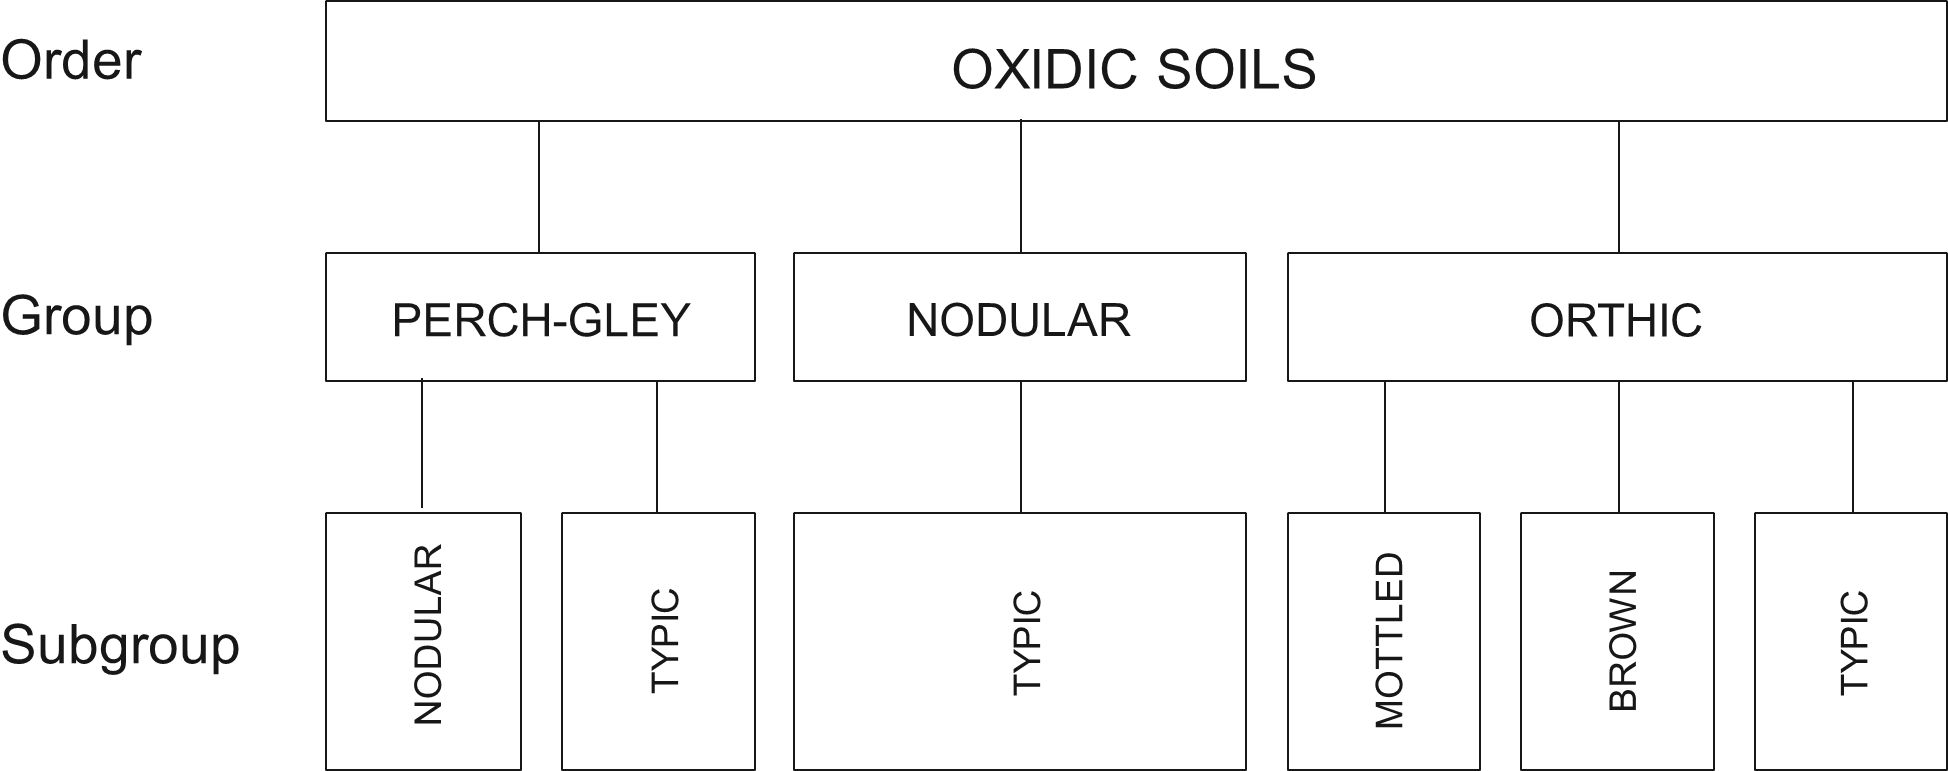
\includegraphics[width=0.85\textwidth,height=\textheight]{./images/Figure-001_oxidic-soils-hierarchy.png}

}

\caption{\label{fig-1}The hierarchy of the
\protect\hyperlink{ord-X}{Oxidic Soils} as an example of the
hierarchical relationships between orders, groups and subgroups. As the
diagram suggests, the range of soil properties for each class is related
to hierarchical position.}

\end{figure}

\hypertarget{sec-intro-misclass}{%
\section{Misclassification}\label{sec-intro-misclass}}

The classes are the most important part of the soil classification. The
key is merely a means of allocating soils to these classes, and by its
nature is imperfect because only a sample of all the possible soils that
might potentially be allocated were used in developing the key.
Consequently, soils will be found that are not allocated to the
appropriate class by the key. This will be apparent when a soil,
allocated to a class, does not conform to the concept and accessory
statements that can normally be made about that class. Because the key
is the servant of the classes, the allocator is justified in placing the
soil misfit into a more appropriate class. If this is done, however, it
must be registered with the person with responsibility for the national
soil classification system, so that appropriate adjustments may be made
to the key when the soil classification is next revised. An allocation
contrary to the key must also be noted in any records or publication of
the allocation.

\hypertarget{sec-intro-new-sgs}{%
\section{Justification of new Subgroups}\label{sec-intro-new-sgs}}

Justification for new subgroups may be made in two ways. First, if a
soil is judged to be misclassified, and a more appropriate class is not
available, then a new subgroup may be justifiable. Second, an existing
subgroup may encompass a set of soils with properties that are too wide
in range. The old subgroup could be split into two new ones. Splitting
may be justified if it will significantly increase the number and
precision of accessory statements that can be made about both of the new
classes.

\hypertarget{sec-intro-correls}{%
\section{Correlations with other soil classification
systems}\label{sec-intro-correls}}

Classes of the New Zealand Soil Classification do not correspond
precisely with classes of other soil classification systems. Despite
this, correlations can be made where classes are substantially
equivalent. In \textbf{?@tbl-1}, classes of the Zealand Soil
Classification are correlated with the New Zealand Genetic Soil
Classification (Taylor and Pohlen 1962) and Soil Taxonomy (Soil Survey
Staff 1999).

\begin{verbatim}
#> Warning: Warning: fonts used in `flextable` are ignored because the `pdflatex`
#> engine is used and not `xelatex` or `lualatex`. You can avoid this warning
#> by using the `set_flextable_defaults(fonts_ignore=TRUE)` command or use a
#> compatible engine by defining `latex_engine: xelatex` in the YAML header of the
#> R Markdown document.
\end{verbatim}

\providecommand{\docline}[3]{\noalign{\global\setlength{\arrayrulewidth}{#1}}\arrayrulecolor[HTML]{#2}\cline{#3}}

\setlength{\tabcolsep}{2pt}

\renewcommand*{\arraystretch}{1.5}

\begin{longtable}[c]{ccc}



\hhline{>{\arrayrulecolor[HTML]{666666}\global\arrayrulewidth=2pt}->{\arrayrulecolor[HTML]{666666}\global\arrayrulewidth=2pt}->{\arrayrulecolor[HTML]{666666}\global\arrayrulewidth=2pt}-}

\multicolumn{1}{!{\color[HTML]{000000}\vrule width 0pt}>{}l}{\fontsize{11}{11}\selectfont{\textcolor[HTML]{000000}{\textbf{NZ\ Soil\ Classification\ (v.\ 3)}}}} & \multicolumn{1}{!{\color[HTML]{000000}\vrule width 0pt}>{}l}{\fontsize{11}{11}\selectfont{\textcolor[HTML]{000000}{\textbf{NZ\ Genetic\ Soil\ Classification}}}} & \multicolumn{1}{!{\color[HTML]{000000}\vrule width 0pt}>{}l!{\color[HTML]{000000}\vrule width 0pt}}{\fontsize{11}{11}\selectfont{\textcolor[HTML]{000000}{\textbf{US\ Soil\ Taxonomy}}}} \\

\hhline{>{\arrayrulecolor[HTML]{666666}\global\arrayrulewidth=2pt}->{\arrayrulecolor[HTML]{666666}\global\arrayrulewidth=2pt}->{\arrayrulecolor[HTML]{666666}\global\arrayrulewidth=2pt}-}

\endfirsthead

\hhline{>{\arrayrulecolor[HTML]{666666}\global\arrayrulewidth=2pt}->{\arrayrulecolor[HTML]{666666}\global\arrayrulewidth=2pt}->{\arrayrulecolor[HTML]{666666}\global\arrayrulewidth=2pt}-}

\multicolumn{1}{!{\color[HTML]{000000}\vrule width 0pt}>{}l}{\fontsize{11}{11}\selectfont{\textcolor[HTML]{000000}{\textbf{NZ\ Soil\ Classification\ (v.\ 3)}}}} & \multicolumn{1}{!{\color[HTML]{000000}\vrule width 0pt}>{}l}{\fontsize{11}{11}\selectfont{\textcolor[HTML]{000000}{\textbf{NZ\ Genetic\ Soil\ Classification}}}} & \multicolumn{1}{!{\color[HTML]{000000}\vrule width 0pt}>{}l!{\color[HTML]{000000}\vrule width 0pt}}{\fontsize{11}{11}\selectfont{\textcolor[HTML]{000000}{\textbf{US\ Soil\ Taxonomy}}}} \\

\hhline{>{\arrayrulecolor[HTML]{666666}\global\arrayrulewidth=2pt}->{\arrayrulecolor[HTML]{666666}\global\arrayrulewidth=2pt}->{\arrayrulecolor[HTML]{666666}\global\arrayrulewidth=2pt}-}\endhead



\multicolumn{3}{!{\color[HTML]{000000}\vrule width 0pt}>{}l!{\color[HTML]{000000}\vrule width 0pt}}{\fontsize{11}{11}\selectfont{\textcolor[HTML]{000000}{\textbf{ALLOPHANIC\ SOILS}}}} \\





\multicolumn{1}{!{\color[HTML]{000000}\vrule width 0pt}>{}l}{\fontsize{11}{11}\selectfont{\textcolor[HTML]{000000}{Perch-Gley\ Allophanic\ Soils}}} & \multicolumn{1}{!{\color[HTML]{000000}\vrule width 0pt}>{}l}{\fontsize{11}{11}\selectfont{\textcolor[HTML]{000000}{gley\ soils}}} & \multicolumn{1}{!{\color[HTML]{000000}\vrule width 0pt}>{}l!{\color[HTML]{000000}\vrule width 0pt}}{\fontsize{11}{11}\selectfont{\textcolor[HTML]{000000}{Aquands}}} \\





\multicolumn{1}{!{\color[HTML]{000000}\vrule width 0pt}>{}l}{\fontsize{11}{11}\selectfont{\textcolor[HTML]{000000}{Gley\ Allophanic\ Soils}}} & \multicolumn{1}{!{\color[HTML]{000000}\vrule width 0pt}>{}l}{\fontsize{11}{11}\selectfont{\textcolor[HTML]{000000}{gley\ soils}}} & \multicolumn{1}{!{\color[HTML]{000000}\vrule width 0pt}>{}l!{\color[HTML]{000000}\vrule width 0pt}}{\fontsize{11}{11}\selectfont{\textcolor[HTML]{000000}{Aquands}}} \\





\multicolumn{1}{!{\color[HTML]{000000}\vrule width 0pt}>{}l}{\fontsize{11}{11}\selectfont{\textcolor[HTML]{000000}{Impeded\ Allophanic\ Soils}}} & \multicolumn{1}{!{\color[HTML]{000000}\vrule width 0pt}>{}l}{\fontsize{11}{11}\selectfont{\textcolor[HTML]{000000}{YB\ loams}}} & \multicolumn{1}{!{\color[HTML]{000000}\vrule width 0pt}>{}l!{\color[HTML]{000000}\vrule width 0pt}}{\fontsize{11}{11}\selectfont{\textcolor[HTML]{000000}{Cryands\ and\ Udands}}} \\





\multicolumn{1}{!{\color[HTML]{000000}\vrule width 0pt}>{}l}{\fontsize{11}{11}\selectfont{\textcolor[HTML]{000000}{Orthic\ Allophanic\ Soils}}} & \multicolumn{1}{!{\color[HTML]{000000}\vrule width 0pt}>{}l}{\fontsize{11}{11}\selectfont{\textcolor[HTML]{000000}{YB\ loams}}} & \multicolumn{1}{!{\color[HTML]{000000}\vrule width 0pt}>{}l!{\color[HTML]{000000}\vrule width 0pt}}{\fontsize{11}{11}\selectfont{\textcolor[HTML]{000000}{Cryands\ and\ Udands}}} \\





\multicolumn{3}{!{\color[HTML]{000000}\vrule width 0pt}>{}l!{\color[HTML]{000000}\vrule width 0pt}}{\fontsize{11}{11}\selectfont{\textcolor[HTML]{000000}{\textbf{ANTHROPIC\ SOILS}}}} \\





\multicolumn{1}{!{\color[HTML]{000000}\vrule width 0pt}>{}l}{\fontsize{11}{11}\selectfont{\textcolor[HTML]{000000}{Truncated\ Anthropic\ Soils}}} & \multicolumn{1}{!{\color[HTML]{000000}\vrule width 0pt}>{}l}{\fontsize{11}{11}\selectfont{\textcolor[HTML]{000000}{anthropic\ soils}}} & \multicolumn{1}{!{\color[HTML]{000000}\vrule width 0pt}>{}l!{\color[HTML]{000000}\vrule width 0pt}}{\fontsize{11}{11}\selectfont{\textcolor[HTML]{000000}{Arents}}} \\





\multicolumn{1}{!{\color[HTML]{000000}\vrule width 0pt}>{}l}{\fontsize{11}{11}\selectfont{\textcolor[HTML]{000000}{Refuse\ Anthropic\ Soils}}} & \multicolumn{1}{!{\color[HTML]{000000}\vrule width 0pt}>{}l}{\fontsize{11}{11}\selectfont{\textcolor[HTML]{000000}{anthropic\ soils}}} & \multicolumn{1}{!{\color[HTML]{000000}\vrule width 0pt}>{}l!{\color[HTML]{000000}\vrule width 0pt}}{\fontsize{11}{11}\selectfont{\textcolor[HTML]{000000}{Arents\ or\ Unclassified}}} \\





\multicolumn{1}{!{\color[HTML]{000000}\vrule width 0pt}>{}l}{\fontsize{11}{11}\selectfont{\textcolor[HTML]{000000}{Mixed\ Anthropic\ Soils}}} & \multicolumn{1}{!{\color[HTML]{000000}\vrule width 0pt}>{}l}{\fontsize{11}{11}\selectfont{\textcolor[HTML]{000000}{anthropic\ soils}}} & \multicolumn{1}{!{\color[HTML]{000000}\vrule width 0pt}>{}l!{\color[HTML]{000000}\vrule width 0pt}}{\fontsize{11}{11}\selectfont{\textcolor[HTML]{000000}{Arents}}} \\





\multicolumn{1}{!{\color[HTML]{000000}\vrule width 0pt}>{}l}{\fontsize{11}{11}\selectfont{\textcolor[HTML]{000000}{Fill\ Anthropic\ Soils}}} & \multicolumn{1}{!{\color[HTML]{000000}\vrule width 0pt}>{}l}{\fontsize{11}{11}\selectfont{\textcolor[HTML]{000000}{anthropic\ soils}}} & \multicolumn{1}{!{\color[HTML]{000000}\vrule width 0pt}>{}l!{\color[HTML]{000000}\vrule width 0pt}}{\fontsize{11}{11}\selectfont{\textcolor[HTML]{000000}{Arents}}} \\





\multicolumn{3}{!{\color[HTML]{000000}\vrule width 0pt}>{}l!{\color[HTML]{000000}\vrule width 0pt}}{\fontsize{11}{11}\selectfont{\textcolor[HTML]{000000}{\textbf{BROWN\ SOILS}}}} \\





\multicolumn{1}{!{\color[HTML]{000000}\vrule width 0pt}>{}l}{\fontsize{11}{11}\selectfont{\textcolor[HTML]{000000}{Allophanic\ Brown\ Soils}}} & \multicolumn{1}{!{\color[HTML]{000000}\vrule width 0pt}>{}l}{\fontsize{11}{11}\selectfont{\textcolor[HTML]{000000}{YB\ earths\ (upland\ \&\ high\ country)}}} & \multicolumn{1}{!{\color[HTML]{000000}\vrule width 0pt}>{}l!{\color[HTML]{000000}\vrule width 0pt}}{\fontsize{11}{11}\selectfont{\textcolor[HTML]{000000}{Dystrochrepts}}} \\





\multicolumn{1}{!{\color[HTML]{000000}\vrule width 0pt}>{}l}{\fontsize{11}{11}\selectfont{\textcolor[HTML]{000000}{Sandy\ Brown\ Soils}}} & \multicolumn{1}{!{\color[HTML]{000000}\vrule width 0pt}>{}l}{\fontsize{11}{11}\selectfont{\textcolor[HTML]{000000}{YB\ sands}}} & \multicolumn{1}{!{\color[HTML]{000000}\vrule width 0pt}>{}l!{\color[HTML]{000000}\vrule width 0pt}}{\fontsize{11}{11}\selectfont{\textcolor[HTML]{000000}{Ustochrepts,\ Dystrochrepts\ and\ Psamments}}} \\





\multicolumn{1}{!{\color[HTML]{000000}\vrule width 0pt}>{}l}{\fontsize{11}{11}\selectfont{\textcolor[HTML]{000000}{Oxidic\ Brown\ Soils}}} & \multicolumn{1}{!{\color[HTML]{000000}\vrule width 0pt}>{}l}{\fontsize{11}{11}\selectfont{\textcolor[HTML]{000000}{YB\ earths\ (northern}}} & \multicolumn{1}{!{\color[HTML]{000000}\vrule width 0pt}>{}l!{\color[HTML]{000000}\vrule width 0pt}}{\fontsize{11}{11}\selectfont{\textcolor[HTML]{000000}{Dsytrochrepts}}} \\





\multicolumn{1}{!{\color[HTML]{000000}\vrule width 0pt}>{}l}{\fontsize{11}{11}\selectfont{\textcolor[HTML]{000000}{Mafic\ Brown\ Soils}}} & \multicolumn{1}{!{\color[HTML]{000000}\vrule width 0pt}>{}l}{\fontsize{11}{11}\selectfont{\textcolor[HTML]{000000}{BG\ loams\ and\ clays}}} & \multicolumn{1}{!{\color[HTML]{000000}\vrule width 0pt}>{}l!{\color[HTML]{000000}\vrule width 0pt}}{\fontsize{11}{11}\selectfont{\textcolor[HTML]{000000}{Dsytrochrepts}}} \\





\multicolumn{1}{!{\color[HTML]{000000}\vrule width 0pt}>{}l}{\fontsize{11}{11}\selectfont{\textcolor[HTML]{000000}{Acid\ Brown\ Soils}}} & \multicolumn{1}{!{\color[HTML]{000000}\vrule width 0pt}>{}l}{\fontsize{11}{11}\selectfont{\textcolor[HTML]{000000}{podzolized\ YB\ earthsor\ YB\ earths}}} & \multicolumn{1}{!{\color[HTML]{000000}\vrule width 0pt}>{}l!{\color[HTML]{000000}\vrule width 0pt}}{\fontsize{11}{11}\selectfont{\textcolor[HTML]{000000}{Dsytrochrepts}}} \\





\multicolumn{1}{!{\color[HTML]{000000}\vrule width 0pt}>{}l}{\fontsize{11}{11}\selectfont{\textcolor[HTML]{000000}{Firm\ Brown\ Soils}}} & \multicolumn{1}{!{\color[HTML]{000000}\vrule width 0pt}>{}l}{\fontsize{11}{11}\selectfont{\textcolor[HTML]{000000}{YB\ earths,\ YB\ shallow\ and\ stony\ soils}}} & \multicolumn{1}{!{\color[HTML]{000000}\vrule width 0pt}>{}l!{\color[HTML]{000000}\vrule width 0pt}}{\fontsize{11}{11}\selectfont{\textcolor[HTML]{000000}{Dystrochrepts\ and\ Ustochrepts}}} \\





\multicolumn{1}{!{\color[HTML]{000000}\vrule width 0pt}>{}l}{\fontsize{11}{11}\selectfont{\textcolor[HTML]{000000}{Orthic\ Brown\ Soils}}} & \multicolumn{1}{!{\color[HTML]{000000}\vrule width 0pt}>{}l}{\fontsize{11}{11}\selectfont{\textcolor[HTML]{000000}{YB\ earths,\ YB\ shallow\ and\ stony\ soils}}} & \multicolumn{1}{!{\color[HTML]{000000}\vrule width 0pt}>{}l!{\color[HTML]{000000}\vrule width 0pt}}{\fontsize{11}{11}\selectfont{\textcolor[HTML]{000000}{Dystrochrepts\ and\ Ustochrepts}}} \\





\multicolumn{3}{!{\color[HTML]{000000}\vrule width 0pt}>{}l!{\color[HTML]{000000}\vrule width 0pt}}{\fontsize{11}{11}\selectfont{\textcolor[HTML]{000000}{\textbf{GLEY\ SOILS}}}} \\





\multicolumn{1}{!{\color[HTML]{000000}\vrule width 0pt}>{}l}{\fontsize{11}{11}\selectfont{\textcolor[HTML]{000000}{Sulpuric\ Gley\ Soils}}} & \multicolumn{1}{!{\color[HTML]{000000}\vrule width 0pt}>{}l}{\fontsize{11}{11}\selectfont{\textcolor[HTML]{000000}{gley\ soils}}} & \multicolumn{1}{!{\color[HTML]{000000}\vrule width 0pt}>{}l!{\color[HTML]{000000}\vrule width 0pt}}{\fontsize{11}{11}\selectfont{\textcolor[HTML]{000000}{Sulphaquepts}}} \\





\multicolumn{1}{!{\color[HTML]{000000}\vrule width 0pt}>{}l}{\fontsize{11}{11}\selectfont{\textcolor[HTML]{000000}{Sandy\ Gley\ Soils}}} & \multicolumn{1}{!{\color[HTML]{000000}\vrule width 0pt}>{}l}{\fontsize{11}{11}\selectfont{\textcolor[HTML]{000000}{gley\ soils}}} & \multicolumn{1}{!{\color[HTML]{000000}\vrule width 0pt}>{}l!{\color[HTML]{000000}\vrule width 0pt}}{\fontsize{11}{11}\selectfont{\textcolor[HTML]{000000}{Aquepts\ or\ Aquents}}} \\





\multicolumn{1}{!{\color[HTML]{000000}\vrule width 0pt}>{}l}{\fontsize{11}{11}\selectfont{\textcolor[HTML]{000000}{Acid\ Gley\ Soils}}} & \multicolumn{1}{!{\color[HTML]{000000}\vrule width 0pt}>{}l}{\fontsize{11}{11}\selectfont{\textcolor[HTML]{000000}{gley\ soils}}} & \multicolumn{1}{!{\color[HTML]{000000}\vrule width 0pt}>{}l!{\color[HTML]{000000}\vrule width 0pt}}{\fontsize{11}{11}\selectfont{\textcolor[HTML]{000000}{Aquepts}}} \\





\multicolumn{1}{!{\color[HTML]{000000}\vrule width 0pt}>{}l}{\fontsize{11}{11}\selectfont{\textcolor[HTML]{000000}{Oxidic\ Gley\ Soils}}} & \multicolumn{1}{!{\color[HTML]{000000}\vrule width 0pt}>{}l}{\fontsize{11}{11}\selectfont{\textcolor[HTML]{000000}{gley\ soils}}} & \multicolumn{1}{!{\color[HTML]{000000}\vrule width 0pt}>{}l!{\color[HTML]{000000}\vrule width 0pt}}{\fontsize{11}{11}\selectfont{\textcolor[HTML]{000000}{Aquox}}} \\





\multicolumn{1}{!{\color[HTML]{000000}\vrule width 0pt}>{}l}{\fontsize{11}{11}\selectfont{\textcolor[HTML]{000000}{Recent\ Gley\ Soils}}} & \multicolumn{1}{!{\color[HTML]{000000}\vrule width 0pt}>{}l}{\fontsize{11}{11}\selectfont{\textcolor[HTML]{000000}{gleyed\ recent\ soils}}} & \multicolumn{1}{!{\color[HTML]{000000}\vrule width 0pt}>{}l!{\color[HTML]{000000}\vrule width 0pt}}{\fontsize{11}{11}\selectfont{\textcolor[HTML]{000000}{Aquents}}} \\





\multicolumn{1}{!{\color[HTML]{000000}\vrule width 0pt}>{}l}{\fontsize{11}{11}\selectfont{\textcolor[HTML]{000000}{Orthic\ Gley\ Soils}}} & \multicolumn{1}{!{\color[HTML]{000000}\vrule width 0pt}>{}l}{\fontsize{11}{11}\selectfont{\textcolor[HTML]{000000}{gleyed\ recent\ soils}}} & \multicolumn{1}{!{\color[HTML]{000000}\vrule width 0pt}>{}l!{\color[HTML]{000000}\vrule width 0pt}}{\fontsize{11}{11}\selectfont{\textcolor[HTML]{000000}{Aquepts\ or\ Aquents}}} \\





\multicolumn{3}{!{\color[HTML]{000000}\vrule width 0pt}>{}l!{\color[HTML]{000000}\vrule width 0pt}}{\fontsize{11}{11}\selectfont{\textcolor[HTML]{000000}{\textbf{GRANULAR\ SOILS}}}} \\





\multicolumn{1}{!{\color[HTML]{000000}\vrule width 0pt}>{}l}{\fontsize{11}{11}\selectfont{\textcolor[HTML]{000000}{Perch-gley\ Granular\ Soils}}} & \multicolumn{1}{!{\color[HTML]{000000}\vrule width 0pt}>{}l}{\fontsize{11}{11}\selectfont{\textcolor[HTML]{000000}{BG\ loams\ or\ BG\ clays}}} & \multicolumn{1}{!{\color[HTML]{000000}\vrule width 0pt}>{}l!{\color[HTML]{000000}\vrule width 0pt}}{\fontsize{11}{11}\selectfont{\textcolor[HTML]{000000}{Aquults}}} \\





\multicolumn{1}{!{\color[HTML]{000000}\vrule width 0pt}>{}l}{\fontsize{11}{11}\selectfont{\textcolor[HTML]{000000}{Melanic\ Granular\ Soils}}} & \multicolumn{1}{!{\color[HTML]{000000}\vrule width 0pt}>{}l}{\fontsize{11}{11}\selectfont{\textcolor[HTML]{000000}{BG\ loams\ or\ BG\ clays}}} & \multicolumn{1}{!{\color[HTML]{000000}\vrule width 0pt}>{}l!{\color[HTML]{000000}\vrule width 0pt}}{\fontsize{11}{11}\selectfont{\textcolor[HTML]{000000}{Humults\ and\ Udalfs}}} \\





\multicolumn{1}{!{\color[HTML]{000000}\vrule width 0pt}>{}l}{\fontsize{11}{11}\selectfont{\textcolor[HTML]{000000}{Oxidic\ Granular\ Soils}}} & \multicolumn{1}{!{\color[HTML]{000000}\vrule width 0pt}>{}l}{\fontsize{11}{11}\selectfont{\textcolor[HTML]{000000}{BG\ loams\ or\ BG\ clays}}} & \multicolumn{1}{!{\color[HTML]{000000}\vrule width 0pt}>{}l!{\color[HTML]{000000}\vrule width 0pt}}{\fontsize{11}{11}\selectfont{\textcolor[HTML]{000000}{Humults}}} \\





\multicolumn{1}{!{\color[HTML]{000000}\vrule width 0pt}>{}l}{\fontsize{11}{11}\selectfont{\textcolor[HTML]{000000}{Orthic\ Granular\ Soils}}} & \multicolumn{1}{!{\color[HTML]{000000}\vrule width 0pt}>{}l}{\fontsize{11}{11}\selectfont{\textcolor[HTML]{000000}{BG\ loams\ or\ BG\ clays}}} & \multicolumn{1}{!{\color[HTML]{000000}\vrule width 0pt}>{}l!{\color[HTML]{000000}\vrule width 0pt}}{\fontsize{11}{11}\selectfont{\textcolor[HTML]{000000}{Humults}}} \\





\multicolumn{3}{!{\color[HTML]{000000}\vrule width 0pt}>{}l!{\color[HTML]{000000}\vrule width 0pt}}{\fontsize{11}{11}\selectfont{\textcolor[HTML]{000000}{\textbf{MELANIC\ SOILS}}}} \\





\multicolumn{1}{!{\color[HTML]{000000}\vrule width 0pt}>{}l}{\fontsize{11}{11}\selectfont{\textcolor[HTML]{000000}{Vertic\ Melanic\ Soils}}} & \multicolumn{1}{!{\color[HTML]{000000}\vrule width 0pt}>{}l}{\fontsize{11}{11}\selectfont{\textcolor[HTML]{000000}{BG\ loams\ and\ clays}}} & \multicolumn{1}{!{\color[HTML]{000000}\vrule width 0pt}>{}l!{\color[HTML]{000000}\vrule width 0pt}}{\fontsize{11}{11}\selectfont{\textcolor[HTML]{000000}{Ustolls\ or\ Vertisols}}} \\





\multicolumn{1}{!{\color[HTML]{000000}\vrule width 0pt}>{}l}{\fontsize{11}{11}\selectfont{\textcolor[HTML]{000000}{Perch-gley\ Melanic\ Soils}}} & \multicolumn{1}{!{\color[HTML]{000000}\vrule width 0pt}>{}l}{\fontsize{11}{11}\selectfont{\textcolor[HTML]{000000}{gley\ soils}}} & \multicolumn{1}{!{\color[HTML]{000000}\vrule width 0pt}>{}l!{\color[HTML]{000000}\vrule width 0pt}}{\fontsize{11}{11}\selectfont{\textcolor[HTML]{000000}{Aquolls}}} \\





\multicolumn{1}{!{\color[HTML]{000000}\vrule width 0pt}>{}l}{\fontsize{11}{11}\selectfont{\textcolor[HTML]{000000}{Rendzic\ Melanic\ Soils}}} & \multicolumn{1}{!{\color[HTML]{000000}\vrule width 0pt}>{}l}{\fontsize{11}{11}\selectfont{\textcolor[HTML]{000000}{rendzinas}}} & \multicolumn{1}{!{\color[HTML]{000000}\vrule width 0pt}>{}l!{\color[HTML]{000000}\vrule width 0pt}}{\fontsize{11}{11}\selectfont{\textcolor[HTML]{000000}{Rendolls}}} \\





\multicolumn{1}{!{\color[HTML]{000000}\vrule width 0pt}>{}l}{\fontsize{11}{11}\selectfont{\textcolor[HTML]{000000}{Mafic\ Melanic\ Soils}}} & \multicolumn{1}{!{\color[HTML]{000000}\vrule width 0pt}>{}l}{\fontsize{11}{11}\selectfont{\textcolor[HTML]{000000}{BG\ loams\ and\ clays}}} & \multicolumn{1}{!{\color[HTML]{000000}\vrule width 0pt}>{}l!{\color[HTML]{000000}\vrule width 0pt}}{\fontsize{11}{11}\selectfont{\textcolor[HTML]{000000}{Ustochrepts,\ Eutrochrepts,\ Ustolls\ or\ Udolls}}} \\





\multicolumn{1}{!{\color[HTML]{000000}\vrule width 0pt}>{}l}{\fontsize{11}{11}\selectfont{\textcolor[HTML]{000000}{Orthic\ Melanic\ Soils}}} & \multicolumn{1}{!{\color[HTML]{000000}\vrule width 0pt}>{}l}{\fontsize{11}{11}\selectfont{\textcolor[HTML]{000000}{rendzinas\ and\ rendzinic\ intergrades}}} & \multicolumn{1}{!{\color[HTML]{000000}\vrule width 0pt}>{}l!{\color[HTML]{000000}\vrule width 0pt}}{\fontsize{11}{11}\selectfont{\textcolor[HTML]{000000}{Ustolls,\ Udolls\ or\ Eutrochrepts}}} \\





\multicolumn{3}{!{\color[HTML]{000000}\vrule width 0pt}>{}l!{\color[HTML]{000000}\vrule width 0pt}}{\fontsize{11}{11}\selectfont{\textcolor[HTML]{000000}{\textbf{ORGANIC\ SOILS}}}} \\





\multicolumn{1}{!{\color[HTML]{000000}\vrule width 0pt}>{}l}{\fontsize{11}{11}\selectfont{\textcolor[HTML]{000000}{Litter\ Organic\ Soils}}} & \multicolumn{1}{!{\color[HTML]{000000}\vrule width 0pt}>{}l}{\fontsize{11}{11}\selectfont{\textcolor[HTML]{000000}{unclassified}}} & \multicolumn{1}{!{\color[HTML]{000000}\vrule width 0pt}>{}l!{\color[HTML]{000000}\vrule width 0pt}}{\fontsize{11}{11}\selectfont{\textcolor[HTML]{000000}{Folists\ or\ unrecognised}}} \\





\multicolumn{1}{!{\color[HTML]{000000}\vrule width 0pt}>{}l}{\fontsize{11}{11}\selectfont{\textcolor[HTML]{000000}{Fibric\ Organic\ Soils}}} & \multicolumn{1}{!{\color[HTML]{000000}\vrule width 0pt}>{}l}{\fontsize{11}{11}\selectfont{\textcolor[HTML]{000000}{organic\ soils}}} & \multicolumn{1}{!{\color[HTML]{000000}\vrule width 0pt}>{}l!{\color[HTML]{000000}\vrule width 0pt}}{\fontsize{11}{11}\selectfont{\textcolor[HTML]{000000}{Fibrists}}} \\





\multicolumn{1}{!{\color[HTML]{000000}\vrule width 0pt}>{}l}{\fontsize{11}{11}\selectfont{\textcolor[HTML]{000000}{Mesic\ Organic\ Soils}}} & \multicolumn{1}{!{\color[HTML]{000000}\vrule width 0pt}>{}l}{\fontsize{11}{11}\selectfont{\textcolor[HTML]{000000}{organic\ soils}}} & \multicolumn{1}{!{\color[HTML]{000000}\vrule width 0pt}>{}l!{\color[HTML]{000000}\vrule width 0pt}}{\fontsize{11}{11}\selectfont{\textcolor[HTML]{000000}{Hemists}}} \\





\multicolumn{1}{!{\color[HTML]{000000}\vrule width 0pt}>{}l}{\fontsize{11}{11}\selectfont{\textcolor[HTML]{000000}{Humic\ Organic\ Soils}}} & \multicolumn{1}{!{\color[HTML]{000000}\vrule width 0pt}>{}l}{\fontsize{11}{11}\selectfont{\textcolor[HTML]{000000}{organic\ soils}}} & \multicolumn{1}{!{\color[HTML]{000000}\vrule width 0pt}>{}l!{\color[HTML]{000000}\vrule width 0pt}}{\fontsize{11}{11}\selectfont{\textcolor[HTML]{000000}{Saprists}}} \\





\multicolumn{3}{!{\color[HTML]{000000}\vrule width 0pt}>{}l!{\color[HTML]{000000}\vrule width 0pt}}{\fontsize{11}{11}\selectfont{\textcolor[HTML]{000000}{\textbf{OXIDIC\ SOILS}}}} \\





\multicolumn{1}{!{\color[HTML]{000000}\vrule width 0pt}>{}l}{\fontsize{11}{11}\selectfont{\textcolor[HTML]{000000}{Perch-gley\ Oxidic\ Soils}}} & \multicolumn{1}{!{\color[HTML]{000000}\vrule width 0pt}>{}l}{\fontsize{11}{11}\selectfont{\textcolor[HTML]{000000}{gley\ soils}}} & \multicolumn{1}{!{\color[HTML]{000000}\vrule width 0pt}>{}l!{\color[HTML]{000000}\vrule width 0pt}}{\fontsize{11}{11}\selectfont{\textcolor[HTML]{000000}{Aquox}}} \\





\multicolumn{1}{!{\color[HTML]{000000}\vrule width 0pt}>{}l}{\fontsize{11}{11}\selectfont{\textcolor[HTML]{000000}{Nodular\ Oxidic\ Soils}}} & \multicolumn{1}{!{\color[HTML]{000000}\vrule width 0pt}>{}l}{} & \multicolumn{1}{!{\color[HTML]{000000}\vrule width 0pt}>{}l!{\color[HTML]{000000}\vrule width 0pt}}{\fontsize{11}{11}\selectfont{\textcolor[HTML]{000000}{Udox}}} \\





\multicolumn{1}{!{\color[HTML]{000000}\vrule width 0pt}>{}l}{\fontsize{11}{11}\selectfont{\textcolor[HTML]{000000}{Orthic\ Oxidic\ Soils}}} & \multicolumn{1}{!{\color[HTML]{000000}\vrule width 0pt}>{}l}{\multirow[c]{-2}{*}{\parbox{0.75in}{\fontsize{11}{11}\selectfont{\textcolor[HTML]{000000}{strongly\ weathered\ red\ loams,\ brown\ loams,\ or\ BG\ loams\ or\ BG\ clays}}}}} & \multicolumn{1}{!{\color[HTML]{000000}\vrule width 0pt}>{}l!{\color[HTML]{000000}\vrule width 0pt}}{\fontsize{11}{11}\selectfont{\textcolor[HTML]{000000}{Udox}}} \\





\multicolumn{3}{!{\color[HTML]{000000}\vrule width 0pt}>{}l!{\color[HTML]{000000}\vrule width 0pt}}{\fontsize{11}{11}\selectfont{\textcolor[HTML]{000000}{\textbf{PALLIC\ SOILS}}}} \\





\multicolumn{1}{!{\color[HTML]{000000}\vrule width 0pt}>{}l}{\fontsize{11}{11}\selectfont{\textcolor[HTML]{000000}{Perch-gley\ Pallic\ Soils}}} & \multicolumn{1}{!{\color[HTML]{000000}\vrule width 0pt}>{}l}{\fontsize{11}{11}\selectfont{\textcolor[HTML]{000000}{yellow-grey\ earths}}} & \multicolumn{1}{!{\color[HTML]{000000}\vrule width 0pt}>{}l!{\color[HTML]{000000}\vrule width 0pt}}{\fontsize{11}{11}\selectfont{\textcolor[HTML]{000000}{Aquepts,\ Aqualfs}}} \\





\multicolumn{1}{!{\color[HTML]{000000}\vrule width 0pt}>{}l}{\fontsize{11}{11}\selectfont{\textcolor[HTML]{000000}{Duric\ Pallic\ Soils}}} & \multicolumn{1}{!{\color[HTML]{000000}\vrule width 0pt}>{}l}{\fontsize{11}{11}\selectfont{\textcolor[HTML]{000000}{yellow-grey\ earths}}} & \multicolumn{1}{!{\color[HTML]{000000}\vrule width 0pt}>{}l!{\color[HTML]{000000}\vrule width 0pt}}{\fontsize{11}{11}\selectfont{\textcolor[HTML]{000000}{Duraqualfs}}} \\





\multicolumn{1}{!{\color[HTML]{000000}\vrule width 0pt}>{}l}{\fontsize{11}{11}\selectfont{\textcolor[HTML]{000000}{Fragic\ Pallic\ Soils}}} & \multicolumn{1}{!{\color[HTML]{000000}\vrule width 0pt}>{}l}{\fontsize{11}{11}\selectfont{\textcolor[HTML]{000000}{yellow-grey\ earths}}} & \multicolumn{1}{!{\color[HTML]{000000}\vrule width 0pt}>{}l!{\color[HTML]{000000}\vrule width 0pt}}{\fontsize{11}{11}\selectfont{\textcolor[HTML]{000000}{Fragiudalfs,\ Fragiochrepts}}} \\





\multicolumn{1}{!{\color[HTML]{000000}\vrule width 0pt}>{}l}{\fontsize{11}{11}\selectfont{\textcolor[HTML]{000000}{Laminar\ Pallic\ Soils}}} & \multicolumn{1}{!{\color[HTML]{000000}\vrule width 0pt}>{}l}{\fontsize{11}{11}\selectfont{\textcolor[HTML]{000000}{yellow-grey\ earths}}} & \multicolumn{1}{!{\color[HTML]{000000}\vrule width 0pt}>{}l!{\color[HTML]{000000}\vrule width 0pt}}{\fontsize{11}{11}\selectfont{\textcolor[HTML]{000000}{Haplustalfs,\ Hapludalfs}}} \\





\multicolumn{1}{!{\color[HTML]{000000}\vrule width 0pt}>{}l}{\fontsize{11}{11}\selectfont{\textcolor[HTML]{000000}{Argillic\ Pallic\ Soils}}} & \multicolumn{1}{!{\color[HTML]{000000}\vrule width 0pt}>{}l}{\fontsize{11}{11}\selectfont{\textcolor[HTML]{000000}{yellow-grey\ earths}}} & \multicolumn{1}{!{\color[HTML]{000000}\vrule width 0pt}>{}l!{\color[HTML]{000000}\vrule width 0pt}}{\fontsize{11}{11}\selectfont{\textcolor[HTML]{000000}{Haplustalfs,\ Hapludalfs}}} \\





\multicolumn{1}{!{\color[HTML]{000000}\vrule width 0pt}>{}l}{\fontsize{11}{11}\selectfont{\textcolor[HTML]{000000}{Immature\ Pallic\ Soils}}} & \multicolumn{1}{!{\color[HTML]{000000}\vrule width 0pt}>{}l}{\fontsize{11}{11}\selectfont{\textcolor[HTML]{000000}{yellow-grey\ earths\ or\ recent\ soils}}} & \multicolumn{1}{!{\color[HTML]{000000}\vrule width 0pt}>{}l!{\color[HTML]{000000}\vrule width 0pt}}{\fontsize{11}{11}\selectfont{\textcolor[HTML]{000000}{Eutrochrepts,\ Ustochrepts}}} \\





\multicolumn{3}{!{\color[HTML]{000000}\vrule width 0pt}>{}l!{\color[HTML]{000000}\vrule width 0pt}}{\fontsize{11}{11}\selectfont{\textcolor[HTML]{000000}{\textbf{PODZOLS}}}} \\





\multicolumn{1}{!{\color[HTML]{000000}\vrule width 0pt}>{}l}{\fontsize{11}{11}\selectfont{\textcolor[HTML]{000000}{Densipan\ Podzols}}} & \multicolumn{1}{!{\color[HTML]{000000}\vrule width 0pt}>{}l}{\fontsize{11}{11}\selectfont{\textcolor[HTML]{000000}{podzols}}} & \multicolumn{1}{!{\color[HTML]{000000}\vrule width 0pt}>{}l!{\color[HTML]{000000}\vrule width 0pt}}{\fontsize{11}{11}\selectfont{\textcolor[HTML]{000000}{Aquods,\ Orthods}}} \\





\multicolumn{1}{!{\color[HTML]{000000}\vrule width 0pt}>{}l}{\fontsize{11}{11}\selectfont{\textcolor[HTML]{000000}{Perch-gley\ Podzols}}} & \multicolumn{1}{!{\color[HTML]{000000}\vrule width 0pt}>{}l}{\fontsize{11}{11}\selectfont{\textcolor[HTML]{000000}{gley\ podzols}}} & \multicolumn{1}{!{\color[HTML]{000000}\vrule width 0pt}>{}l!{\color[HTML]{000000}\vrule width 0pt}}{\fontsize{11}{11}\selectfont{\textcolor[HTML]{000000}{Aquods}}} \\





\multicolumn{1}{!{\color[HTML]{000000}\vrule width 0pt}>{}l}{\fontsize{11}{11}\selectfont{\textcolor[HTML]{000000}{Groundwater-gley\ Podzols}}} & \multicolumn{1}{!{\color[HTML]{000000}\vrule width 0pt}>{}l}{\fontsize{11}{11}\selectfont{\textcolor[HTML]{000000}{gley\ podzols}}} & \multicolumn{1}{!{\color[HTML]{000000}\vrule width 0pt}>{}l!{\color[HTML]{000000}\vrule width 0pt}}{\fontsize{11}{11}\selectfont{\textcolor[HTML]{000000}{Aquods}}} \\





\multicolumn{1}{!{\color[HTML]{000000}\vrule width 0pt}>{}l}{\fontsize{11}{11}\selectfont{\textcolor[HTML]{000000}{Pan\ Podzols}}} & \multicolumn{1}{!{\color[HTML]{000000}\vrule width 0pt}>{}l}{\fontsize{11}{11}\selectfont{\textcolor[HTML]{000000}{podzols}}} & \multicolumn{1}{!{\color[HTML]{000000}\vrule width 0pt}>{}l!{\color[HTML]{000000}\vrule width 0pt}}{\fontsize{11}{11}\selectfont{\textcolor[HTML]{000000}{Orthods}}} \\





\multicolumn{1}{!{\color[HTML]{000000}\vrule width 0pt}>{}l}{\fontsize{11}{11}\selectfont{\textcolor[HTML]{000000}{Orthic\ Podzols}}} & \multicolumn{1}{!{\color[HTML]{000000}\vrule width 0pt}>{}l}{\fontsize{11}{11}\selectfont{\textcolor[HTML]{000000}{podzols}}} & \multicolumn{1}{!{\color[HTML]{000000}\vrule width 0pt}>{}l!{\color[HTML]{000000}\vrule width 0pt}}{\fontsize{11}{11}\selectfont{\textcolor[HTML]{000000}{Orthods}}} \\





\multicolumn{3}{!{\color[HTML]{000000}\vrule width 0pt}>{}l!{\color[HTML]{000000}\vrule width 0pt}}{\fontsize{11}{11}\selectfont{\textcolor[HTML]{000000}{\textbf{PUMICE\ SOILS}}}} \\





\multicolumn{1}{!{\color[HTML]{000000}\vrule width 0pt}>{}l}{\fontsize{11}{11}\selectfont{\textcolor[HTML]{000000}{Perch-gley\ Pumice\ Soils}}} & \multicolumn{1}{!{\color[HTML]{000000}\vrule width 0pt}>{}l}{\fontsize{11}{11}\selectfont{\textcolor[HTML]{000000}{gley\ soils}}} & \multicolumn{1}{!{\color[HTML]{000000}\vrule width 0pt}>{}l!{\color[HTML]{000000}\vrule width 0pt}}{\fontsize{11}{11}\selectfont{\textcolor[HTML]{000000}{Vitraquands}}} \\





\multicolumn{1}{!{\color[HTML]{000000}\vrule width 0pt}>{}l}{\fontsize{11}{11}\selectfont{\textcolor[HTML]{000000}{Impeded\ Pumice\ Soils}}} & \multicolumn{1}{!{\color[HTML]{000000}\vrule width 0pt}>{}l}{\fontsize{11}{11}\selectfont{\textcolor[HTML]{000000}{YB\ pumice\ soils}}} & \multicolumn{1}{!{\color[HTML]{000000}\vrule width 0pt}>{}l!{\color[HTML]{000000}\vrule width 0pt}}{\fontsize{11}{11}\selectfont{\textcolor[HTML]{000000}{Vitrands,\ Vitricryands}}} \\





\multicolumn{1}{!{\color[HTML]{000000}\vrule width 0pt}>{}l}{\fontsize{11}{11}\selectfont{\textcolor[HTML]{000000}{Orthic\ Pumice\ Soils}}} & \multicolumn{1}{!{\color[HTML]{000000}\vrule width 0pt}>{}l}{\fontsize{11}{11}\selectfont{\textcolor[HTML]{000000}{YB\ pumice\ soils}}} & \multicolumn{1}{!{\color[HTML]{000000}\vrule width 0pt}>{}l!{\color[HTML]{000000}\vrule width 0pt}}{\fontsize{11}{11}\selectfont{\textcolor[HTML]{000000}{Vitrands,\ Vitricryands}}} \\





\multicolumn{3}{!{\color[HTML]{000000}\vrule width 0pt}>{}l!{\color[HTML]{000000}\vrule width 0pt}}{\fontsize{11}{11}\selectfont{\textcolor[HTML]{000000}{\textbf{RAW\ SOILS}}}} \\





\multicolumn{1}{!{\color[HTML]{000000}\vrule width 0pt}>{}l}{\fontsize{11}{11}\selectfont{\textcolor[HTML]{000000}{Gley\ Raw\ Soils}}} & \multicolumn{1}{!{\color[HTML]{000000}\vrule width 0pt}>{}l}{\fontsize{11}{11}\selectfont{\textcolor[HTML]{000000}{unclassified}}} & \multicolumn{1}{!{\color[HTML]{000000}\vrule width 0pt}>{}l!{\color[HTML]{000000}\vrule width 0pt}}{\fontsize{11}{11}\selectfont{\textcolor[HTML]{000000}{Entisols,\ or\ not-soil}}} \\





\multicolumn{1}{!{\color[HTML]{000000}\vrule width 0pt}>{}l}{\fontsize{11}{11}\selectfont{\textcolor[HTML]{000000}{Hydrothermal\ Raw\ Soils}}} & \multicolumn{1}{!{\color[HTML]{000000}\vrule width 0pt}>{}l}{\fontsize{11}{11}\selectfont{\textcolor[HTML]{000000}{hydrothermal\ soils}}} & \multicolumn{1}{!{\color[HTML]{000000}\vrule width 0pt}>{}l!{\color[HTML]{000000}\vrule width 0pt}}{\fontsize{11}{11}\selectfont{\textcolor[HTML]{000000}{Entisols,\ or\ not-soil}}} \\





\multicolumn{1}{!{\color[HTML]{000000}\vrule width 0pt}>{}l}{\fontsize{11}{11}\selectfont{\textcolor[HTML]{000000}{Rocky\ Raw\ Soils}}} & \multicolumn{1}{!{\color[HTML]{000000}\vrule width 0pt}>{}l}{\fontsize{11}{11}\selectfont{\textcolor[HTML]{000000}{unclassified}}} & \multicolumn{1}{!{\color[HTML]{000000}\vrule width 0pt}>{}l!{\color[HTML]{000000}\vrule width 0pt}}{\fontsize{11}{11}\selectfont{\textcolor[HTML]{000000}{Entisols,\ or\ not-soil}}} \\





\multicolumn{1}{!{\color[HTML]{000000}\vrule width 0pt}>{}l}{\fontsize{11}{11}\selectfont{\textcolor[HTML]{000000}{Sandy\ Raw\ Soils}}} & \multicolumn{1}{!{\color[HTML]{000000}\vrule width 0pt}>{}l}{\fontsize{11}{11}\selectfont{\textcolor[HTML]{000000}{unclassified}}} & \multicolumn{1}{!{\color[HTML]{000000}\vrule width 0pt}>{}l!{\color[HTML]{000000}\vrule width 0pt}}{\fontsize{11}{11}\selectfont{\textcolor[HTML]{000000}{Entisols,\ or\ not-soil}}} \\





\multicolumn{1}{!{\color[HTML]{000000}\vrule width 0pt}>{}l}{\fontsize{11}{11}\selectfont{\textcolor[HTML]{000000}{Fluvial\ Raw\ Soils}}} & \multicolumn{1}{!{\color[HTML]{000000}\vrule width 0pt}>{}l}{\fontsize{11}{11}\selectfont{\textcolor[HTML]{000000}{unclassified}}} & \multicolumn{1}{!{\color[HTML]{000000}\vrule width 0pt}>{}l!{\color[HTML]{000000}\vrule width 0pt}}{\fontsize{11}{11}\selectfont{\textcolor[HTML]{000000}{Entisols,\ or\ not-soil}}} \\





\multicolumn{1}{!{\color[HTML]{000000}\vrule width 0pt}>{}l}{\fontsize{11}{11}\selectfont{\textcolor[HTML]{000000}{Tephric\ Raw\ Soils}}} & \multicolumn{1}{!{\color[HTML]{000000}\vrule width 0pt}>{}l}{\fontsize{11}{11}\selectfont{\textcolor[HTML]{000000}{unclassified}}} & \multicolumn{1}{!{\color[HTML]{000000}\vrule width 0pt}>{}l!{\color[HTML]{000000}\vrule width 0pt}}{\fontsize{11}{11}\selectfont{\textcolor[HTML]{000000}{Entisols,\ or\ not-soil}}} \\





\multicolumn{1}{!{\color[HTML]{000000}\vrule width 0pt}>{}l}{\fontsize{11}{11}\selectfont{\textcolor[HTML]{000000}{Orthic\ Raw\ Soils}}} & \multicolumn{1}{!{\color[HTML]{000000}\vrule width 0pt}>{}l}{\fontsize{11}{11}\selectfont{\textcolor[HTML]{000000}{unclassified}}} & \multicolumn{1}{!{\color[HTML]{000000}\vrule width 0pt}>{}l!{\color[HTML]{000000}\vrule width 0pt}}{\fontsize{11}{11}\selectfont{\textcolor[HTML]{000000}{Entisols,\ or\ not-soil}}} \\





\multicolumn{3}{!{\color[HTML]{000000}\vrule width 0pt}>{}l!{\color[HTML]{000000}\vrule width 0pt}}{\fontsize{11}{11}\selectfont{\textcolor[HTML]{000000}{\textbf{RECENT\ SOILS}}}} \\





\multicolumn{1}{!{\color[HTML]{000000}\vrule width 0pt}>{}l}{\fontsize{11}{11}\selectfont{\textcolor[HTML]{000000}{Hydrothermal\ Recent\ Soils}}} & \multicolumn{1}{!{\color[HTML]{000000}\vrule width 0pt}>{}l}{\fontsize{11}{11}\selectfont{\textcolor[HTML]{000000}{recent\ soils}}} & \multicolumn{1}{!{\color[HTML]{000000}\vrule width 0pt}>{}l!{\color[HTML]{000000}\vrule width 0pt}}{\fontsize{11}{11}\selectfont{\textcolor[HTML]{000000}{Aquents,\ Orthents}}} \\





\multicolumn{1}{!{\color[HTML]{000000}\vrule width 0pt}>{}l}{\fontsize{11}{11}\selectfont{\textcolor[HTML]{000000}{Rocky\ Recent\ Soils}}} & \multicolumn{1}{!{\color[HTML]{000000}\vrule width 0pt}>{}l}{\fontsize{11}{11}\selectfont{\textcolor[HTML]{000000}{lithosols}}} & \multicolumn{1}{!{\color[HTML]{000000}\vrule width 0pt}>{}l!{\color[HTML]{000000}\vrule width 0pt}}{\fontsize{11}{11}\selectfont{\textcolor[HTML]{000000}{Orthents}}} \\





\multicolumn{1}{!{\color[HTML]{000000}\vrule width 0pt}>{}l}{\fontsize{11}{11}\selectfont{\textcolor[HTML]{000000}{Sandy\ Recent\ Soils}}} & \multicolumn{1}{!{\color[HTML]{000000}\vrule width 0pt}>{}l}{\fontsize{11}{11}\selectfont{\textcolor[HTML]{000000}{recent\ soils}}} & \multicolumn{1}{!{\color[HTML]{000000}\vrule width 0pt}>{}l!{\color[HTML]{000000}\vrule width 0pt}}{\fontsize{11}{11}\selectfont{\textcolor[HTML]{000000}{Psamments}}} \\





\multicolumn{1}{!{\color[HTML]{000000}\vrule width 0pt}>{}l}{\fontsize{11}{11}\selectfont{\textcolor[HTML]{000000}{Fluvial\ Recent\ Soils}}} & \multicolumn{1}{!{\color[HTML]{000000}\vrule width 0pt}>{}l}{\fontsize{11}{11}\selectfont{\textcolor[HTML]{000000}{recent\ soils}}} & \multicolumn{1}{!{\color[HTML]{000000}\vrule width 0pt}>{}l!{\color[HTML]{000000}\vrule width 0pt}}{\fontsize{11}{11}\selectfont{\textcolor[HTML]{000000}{Fluvents,\ Ochrepts}}} \\





\multicolumn{1}{!{\color[HTML]{000000}\vrule width 0pt}>{}l}{\fontsize{11}{11}\selectfont{\textcolor[HTML]{000000}{Tephric\ Recent\ Soils}}} & \multicolumn{1}{!{\color[HTML]{000000}\vrule width 0pt}>{}l}{\fontsize{11}{11}\selectfont{\textcolor[HTML]{000000}{recent\ soils}}} & \multicolumn{1}{!{\color[HTML]{000000}\vrule width 0pt}>{}l!{\color[HTML]{000000}\vrule width 0pt}}{\fontsize{11}{11}\selectfont{\textcolor[HTML]{000000}{Orthents,\ Cryands,\ Udands}}} \\





\multicolumn{1}{!{\color[HTML]{000000}\vrule width 0pt}>{}l}{\fontsize{11}{11}\selectfont{\textcolor[HTML]{000000}{Orthic\ Recent\ Soils}}} & \multicolumn{1}{!{\color[HTML]{000000}\vrule width 0pt}>{}l}{\fontsize{11}{11}\selectfont{\textcolor[HTML]{000000}{recent\ soils}}} & \multicolumn{1}{!{\color[HTML]{000000}\vrule width 0pt}>{}l!{\color[HTML]{000000}\vrule width 0pt}}{\fontsize{11}{11}\selectfont{\textcolor[HTML]{000000}{Orthents,\ Ochrepts}}} \\





\multicolumn{3}{!{\color[HTML]{000000}\vrule width 0pt}>{}l!{\color[HTML]{000000}\vrule width 0pt}}{\fontsize{11}{11}\selectfont{\textcolor[HTML]{000000}{\textbf{SEMIARID\ SOILS}}}} \\





\multicolumn{1}{!{\color[HTML]{000000}\vrule width 0pt}>{}l}{\fontsize{11}{11}\selectfont{\textcolor[HTML]{000000}{Aged-argillic\ Semiarid\ Soils}}} & \multicolumn{1}{!{\color[HTML]{000000}\vrule width 0pt}>{}l}{\fontsize{11}{11}\selectfont{\textcolor[HTML]{000000}{brown-grey\ earths}}} & \multicolumn{1}{!{\color[HTML]{000000}\vrule width 0pt}>{}l!{\color[HTML]{000000}\vrule width 0pt}}{\fontsize{11}{11}\selectfont{\textcolor[HTML]{000000}{Haplargids}}} \\





\multicolumn{1}{!{\color[HTML]{000000}\vrule width 0pt}>{}l}{\fontsize{11}{11}\selectfont{\textcolor[HTML]{000000}{Solonetzic\ Semiarid\ Soils}}} & \multicolumn{1}{!{\color[HTML]{000000}\vrule width 0pt}>{}l}{\fontsize{11}{11}\selectfont{\textcolor[HTML]{000000}{solonetz}}} & \multicolumn{1}{!{\color[HTML]{000000}\vrule width 0pt}>{}l!{\color[HTML]{000000}\vrule width 0pt}}{\fontsize{11}{11}\selectfont{\textcolor[HTML]{000000}{Natragids}}} \\





\multicolumn{1}{!{\color[HTML]{000000}\vrule width 0pt}>{}l}{\fontsize{11}{11}\selectfont{\textcolor[HTML]{000000}{Argillic\ Semiarid\ Soils}}} & \multicolumn{1}{!{\color[HTML]{000000}\vrule width 0pt}>{}l}{\fontsize{11}{11}\selectfont{\textcolor[HTML]{000000}{brown-grey\ earths}}} & \multicolumn{1}{!{\color[HTML]{000000}\vrule width 0pt}>{}l!{\color[HTML]{000000}\vrule width 0pt}}{\fontsize{11}{11}\selectfont{\textcolor[HTML]{000000}{Haplargids,}}} \\





\multicolumn{1}{!{\color[HTML]{000000}\vrule width 0pt}>{}l}{\fontsize{11}{11}\selectfont{\textcolor[HTML]{000000}{Immature\ Semiarid\ Soils}}} & \multicolumn{1}{!{\color[HTML]{000000}\vrule width 0pt}>{}l}{\fontsize{11}{11}\selectfont{\textcolor[HTML]{000000}{brown-grey\ earths}}} & \multicolumn{1}{!{\color[HTML]{000000}\vrule width 0pt}>{}l!{\color[HTML]{000000}\vrule width 0pt}}{\fontsize{11}{11}\selectfont{\textcolor[HTML]{000000}{Camborthids}}} \\





\multicolumn{3}{!{\color[HTML]{000000}\vrule width 0pt}>{}l!{\color[HTML]{000000}\vrule width 0pt}}{\fontsize{11}{11}\selectfont{\textcolor[HTML]{000000}{\textbf{ULTIC\ SOILS}}}} \\





\multicolumn{1}{!{\color[HTML]{000000}\vrule width 0pt}>{}l}{\fontsize{11}{11}\selectfont{\textcolor[HTML]{000000}{Densipan\ Ultic\ Soils}}} & \multicolumn{1}{!{\color[HTML]{000000}\vrule width 0pt}>{}l}{\fontsize{11}{11}\selectfont{\textcolor[HTML]{000000}{YB\ earths\ or\ podzols}}} & \multicolumn{1}{!{\color[HTML]{000000}\vrule width 0pt}>{}l!{\color[HTML]{000000}\vrule width 0pt}}{\fontsize{11}{11}\selectfont{\textcolor[HTML]{000000}{Aquults}}} \\





\multicolumn{1}{!{\color[HTML]{000000}\vrule width 0pt}>{}l}{\fontsize{11}{11}\selectfont{\textcolor[HTML]{000000}{Albic\ Ultic\ Soils}}} & \multicolumn{1}{!{\color[HTML]{000000}\vrule width 0pt}>{}l}{\fontsize{11}{11}\selectfont{\textcolor[HTML]{000000}{YB\ earths}}} & \multicolumn{1}{!{\color[HTML]{000000}\vrule width 0pt}>{}l!{\color[HTML]{000000}\vrule width 0pt}}{\fontsize{11}{11}\selectfont{\textcolor[HTML]{000000}{Aquults,\ Humults\ or\ Udults}}} \\





\multicolumn{1}{!{\color[HTML]{000000}\vrule width 0pt}>{}l}{\fontsize{11}{11}\selectfont{\textcolor[HTML]{000000}{Perch-gley\ Ultic\ Soils}}} & \multicolumn{1}{!{\color[HTML]{000000}\vrule width 0pt}>{}l}{\fontsize{11}{11}\selectfont{\textcolor[HTML]{000000}{YB\ earths}}} & \multicolumn{1}{!{\color[HTML]{000000}\vrule width 0pt}>{}l!{\color[HTML]{000000}\vrule width 0pt}}{\fontsize{11}{11}\selectfont{\textcolor[HTML]{000000}{Aquults}}} \\





\multicolumn{1}{!{\color[HTML]{000000}\vrule width 0pt}>{}l}{\fontsize{11}{11}\selectfont{\textcolor[HTML]{000000}{Sandy\ Ultic\ Soils}}} & \multicolumn{1}{!{\color[HTML]{000000}\vrule width 0pt}>{}l}{\fontsize{11}{11}\selectfont{\textcolor[HTML]{000000}{YB\ earths\ or\ YB\ sands}}} & \multicolumn{1}{!{\color[HTML]{000000}\vrule width 0pt}>{}l!{\color[HTML]{000000}\vrule width 0pt}}{\fontsize{11}{11}\selectfont{\textcolor[HTML]{000000}{Hapludults}}} \\





\multicolumn{1}{!{\color[HTML]{000000}\vrule width 0pt}>{}l}{\fontsize{11}{11}\selectfont{\textcolor[HTML]{000000}{Yellow\ Ultic\ Soils}}} & \multicolumn{1}{!{\color[HTML]{000000}\vrule width 0pt}>{}l}{\fontsize{11}{11}\selectfont{\textcolor[HTML]{000000}{YB\ earths}}} & \multicolumn{1}{!{\color[HTML]{000000}\vrule width 0pt}>{}l!{\color[HTML]{000000}\vrule width 0pt}}{\fontsize{11}{11}\selectfont{\textcolor[HTML]{000000}{Hapludults}}} \\

\hhline{>{\arrayrulecolor[HTML]{666666}\global\arrayrulewidth=2pt}->{\arrayrulecolor[HTML]{666666}\global\arrayrulewidth=2pt}->{\arrayrulecolor[HTML]{666666}\global\arrayrulewidth=2pt}-}



\end{longtable}

\bookmarksetup{startatroot}

\hypertarget{sec-diagnostics}{%
\chapter{Diagnostic horizons and other
differentiae}\label{sec-diagnostics}}

Diagnostic horizons and other differentiating criteria are defined to
facilitate the assignment of soils to classes. The definitions are not
intended to represent a comprehensive classification of horizons. A
summary of these is given below.

\begin{verbatim}
#> Warning: Warning: fonts used in `flextable` are ignored because the `pdflatex`
#> engine is used and not `xelatex` or `lualatex`. You can avoid this warning
#> by using the `set_flextable_defaults(fonts_ignore=TRUE)` command or use a
#> compatible engine by defining `latex_engine: xelatex` in the YAML header of the
#> R Markdown document.
\end{verbatim}

\providecommand{\docline}[3]{\noalign{\global\setlength{\arrayrulewidth}{#1}}\arrayrulecolor[HTML]{#2}\cline{#3}}

\setlength{\tabcolsep}{2pt}

\renewcommand*{\arraystretch}{1.5}

\begin{longtable}[c]{cc}





\endfirsthead

\hhline{~~}

\multicolumn{1}{!{\color[HTML]{000000}\vrule width 0pt}>{}l}{\fontsize{11}{11}\selectfont{\textcolor[HTML]{000000}{\textbf{Horizons,\ Pans\ and}}}\fontsize{11}{11}\selectfont{\textcolor[HTML]{000000}{\textbf{\linebreak }}}\fontsize{11}{11}\selectfont{\textcolor[HTML]{000000}{\textbf{\ Layers:}}}} & \multicolumn{1}{!{\color[HTML]{000000}\vrule width 0pt}>{}l!{\color[HTML]{000000}\vrule width 0pt}}{\fontsize{11}{11}\selectfont{\textcolor[HTML]{000000}{\textbf{Soil\ materials\ and}}}\fontsize{11}{11}\selectfont{\textcolor[HTML]{000000}{\textbf{\linebreak }}}\fontsize{11}{11}\selectfont{\textcolor[HTML]{000000}{\textbf{\ Contacts:}}}} \\





\multicolumn{1}{!{\color[HTML]{000000}\vrule width 0pt}>{}l}{\fontsize{11}{11}\selectfont{\textcolor[HTML]{000000}{Argillic\ horizon}}} & \multicolumn{1}{!{\color[HTML]{000000}\vrule width 0pt}>{}l!{\color[HTML]{000000}\vrule width 0pt}}{\fontsize{11}{11}\selectfont{\textcolor[HTML]{000000}{Allophanic\ soil\ material}}} \\





\multicolumn{1}{!{\color[HTML]{000000}\vrule width 0pt}>{}l}{\fontsize{11}{11}\selectfont{\textcolor[HTML]{000000}{Brittle-B\ horizon}}} & \multicolumn{1}{!{\color[HTML]{000000}\vrule width 0pt}>{}l!{\color[HTML]{000000}\vrule width 0pt}}{\fontsize{11}{11}\selectfont{\textcolor[HTML]{000000}{Lithic\ contact}}} \\





\multicolumn{1}{!{\color[HTML]{000000}\vrule width 0pt}>{}l}{\fontsize{11}{11}\selectfont{\textcolor[HTML]{000000}{Calcareous\ horizon}}} & \multicolumn{1}{!{\color[HTML]{000000}\vrule width 0pt}>{}l!{\color[HTML]{000000}\vrule width 0pt}}{\fontsize{11}{11}\selectfont{\textcolor[HTML]{000000}{Organic\ soil\ material}}} \\





\multicolumn{1}{!{\color[HTML]{000000}\vrule width 0pt}>{}l}{\fontsize{11}{11}\selectfont{\textcolor[HTML]{000000}{Cutanic\ horizon}}} & \multicolumn{1}{!{\color[HTML]{000000}\vrule width 0pt}>{}l!{\color[HTML]{000000}\vrule width 0pt}}{\fontsize{11}{11}\selectfont{\textcolor[HTML]{000000}{Paralithic\ contact}}} \\





\multicolumn{1}{!{\color[HTML]{000000}\vrule width 0pt}>{}l}{\fontsize{11}{11}\selectfont{\textcolor[HTML]{000000}{Cutanoxidic\ horizon}}} & \multicolumn{1}{!{\color[HTML]{000000}\vrule width 0pt}>{}l!{\color[HTML]{000000}\vrule width 0pt}}{\fontsize{11}{11}\selectfont{\textcolor[HTML]{000000}{Tephric\ soil\ material}}} \\





\multicolumn{1}{!{\color[HTML]{000000}\vrule width 0pt}>{}l}{\fontsize{11}{11}\selectfont{\textcolor[HTML]{000000}{Densipan}}} & \multicolumn{1}{!{\color[HTML]{000000}\vrule width 0pt}>{}l!{\color[HTML]{000000}\vrule width 0pt}}{\fontsize{11}{11}\selectfont{\textcolor[HTML]{000000}{Vitric\ soil\ material}}} \\





\multicolumn{1}{!{\color[HTML]{000000}\vrule width 0pt}>{}l}{\fontsize{11}{11}\selectfont{\textcolor[HTML]{000000}{Duripan}}} & \multicolumn{1}{!{\color[HTML]{000000}\vrule width 0pt}>{}l!{\color[HTML]{000000}\vrule width 0pt}}{\fontsize{11}{11}\selectfont{\textcolor[HTML]{000000}{}}} \\





\multicolumn{1}{!{\color[HTML]{000000}\vrule width 0pt}>{}l}{\fontsize{11}{11}\selectfont{\textcolor[HTML]{000000}{Distinct\ topsoil}}} & \multicolumn{1}{!{\color[HTML]{000000}\vrule width 0pt}>{}l!{\color[HTML]{000000}\vrule width 0pt}}{\fontsize{11}{11}\selectfont{\textcolor[HTML]{000000}{\textbf{Profile\ Forms:}}}} \\





\multicolumn{1}{!{\color[HTML]{000000}\vrule width 0pt}>{}l}{\fontsize{11}{11}\selectfont{\textcolor[HTML]{000000}{Fragipan}}} & \multicolumn{1}{!{\color[HTML]{000000}\vrule width 0pt}>{}l!{\color[HTML]{000000}\vrule width 0pt}}{\fontsize{11}{11}\selectfont{\textcolor[HTML]{000000}{Gley\ profile\ form}}} \\





\multicolumn{1}{!{\color[HTML]{000000}\vrule width 0pt}>{}l}{\fontsize{11}{11}\selectfont{\textcolor[HTML]{000000}{Humus-pan}}} & \multicolumn{1}{!{\color[HTML]{000000}\vrule width 0pt}>{}l!{\color[HTML]{000000}\vrule width 0pt}}{\fontsize{11}{11}\selectfont{\textcolor[HTML]{000000}{Mottled\ profile\ form}}} \\





\multicolumn{1}{!{\color[HTML]{000000}\vrule width 0pt}>{}l}{\fontsize{11}{11}\selectfont{\textcolor[HTML]{000000}{Ironstone-pan}}} & \multicolumn{1}{!{\color[HTML]{000000}\vrule width 0pt}>{}l!{\color[HTML]{000000}\vrule width 0pt}}{\fontsize{11}{11}\selectfont{\textcolor[HTML]{000000}{}}} \\





\multicolumn{1}{!{\color[HTML]{000000}\vrule width 0pt}>{}l}{\fontsize{11}{11}\selectfont{\textcolor[HTML]{000000}{Nodular\ horizon}}} & \multicolumn{1}{!{\color[HTML]{000000}\vrule width 0pt}>{}l!{\color[HTML]{000000}\vrule width 0pt}}{\fontsize{11}{11}\selectfont{\textcolor[HTML]{000000}{\textbf{Features:}}}} \\





\multicolumn{1}{!{\color[HTML]{000000}\vrule width 0pt}>{}l}{\fontsize{11}{11}\selectfont{\textcolor[HTML]{000000}{Ortstein-pan}}} & \multicolumn{1}{!{\color[HTML]{000000}\vrule width 0pt}>{}l!{\color[HTML]{000000}\vrule width 0pt}}{\fontsize{11}{11}\selectfont{\textcolor[HTML]{000000}{Fluvial\ features}}} \\





\multicolumn{1}{!{\color[HTML]{000000}\vrule width 0pt}>{}l}{\fontsize{11}{11}\selectfont{\textcolor[HTML]{000000}{Oxidic\ horizon}}} & \multicolumn{1}{!{\color[HTML]{000000}\vrule width 0pt}>{}l!{\color[HTML]{000000}\vrule width 0pt}}{\fontsize{11}{11}\selectfont{\textcolor[HTML]{000000}{Perch-gley\ features}}} \\





\multicolumn{1}{!{\color[HTML]{000000}\vrule width 0pt}>{}l}{\fontsize{11}{11}\selectfont{\textcolor[HTML]{000000}{Peaty\ topsoil}}} & \multicolumn{1}{!{\color[HTML]{000000}\vrule width 0pt}>{}l!{\color[HTML]{000000}\vrule width 0pt}}{\fontsize{11}{11}\selectfont{\textcolor[HTML]{000000}{Sodic\ features}}} \\





\multicolumn{1}{!{\color[HTML]{000000}\vrule width 0pt}>{}l}{\fontsize{11}{11}\selectfont{\textcolor[HTML]{000000}{Placic\ horizon}}} & \multicolumn{1}{!{\color[HTML]{000000}\vrule width 0pt}>{}l!{\color[HTML]{000000}\vrule width 0pt}}{\fontsize{11}{11}\selectfont{\textcolor[HTML]{000000}{}}} \\





\multicolumn{1}{!{\color[HTML]{000000}\vrule width 0pt}>{}l}{\fontsize{11}{11}\selectfont{\textcolor[HTML]{000000}{Podzolic-B\ horizon}}} & \multicolumn{1}{!{\color[HTML]{000000}\vrule width 0pt}>{}l!{\color[HTML]{000000}\vrule width 0pt}}{\fontsize{11}{11}\selectfont{\textcolor[HTML]{000000}{\textbf{Other\ Differentiae:}}}} \\





\multicolumn{1}{!{\color[HTML]{000000}\vrule width 0pt}>{}l}{\fontsize{11}{11}\selectfont{\textcolor[HTML]{000000}{Reductimorphic\ horizon}}} & \multicolumn{1}{!{\color[HTML]{000000}\vrule width 0pt}>{}l!{\color[HTML]{000000}\vrule width 0pt}}{\fontsize{11}{11}\selectfont{\textcolor[HTML]{000000}{Crumb\ structure}}} \\





\multicolumn{1}{!{\color[HTML]{000000}\vrule width 0pt}>{}l}{\fontsize{11}{11}\selectfont{\textcolor[HTML]{000000}{Redox-mottled\ horizon}}} & \multicolumn{1}{!{\color[HTML]{000000}\vrule width 0pt}>{}l!{\color[HTML]{000000}\vrule width 0pt}}{\fontsize{11}{11}\selectfont{\textcolor[HTML]{000000}{Reactive-aluminium\ test}}} \\





\multicolumn{1}{!{\color[HTML]{000000}\vrule width 0pt}>{}l}{\fontsize{11}{11}\selectfont{\textcolor[HTML]{000000}{Slowly\ permeable\ layer}}} & \multicolumn{1}{!{\color[HTML]{000000}\vrule width 0pt}>{}l!{\color[HTML]{000000}\vrule width 0pt}}{\fontsize{11}{11}\selectfont{\textcolor[HTML]{000000}{Redox\ segregations}}} \\





\multicolumn{1}{!{\color[HTML]{000000}\vrule width 0pt}>{}l}{\fontsize{11}{11}\selectfont{\textcolor[HTML]{000000}{Weathered-B\ horizon}}} & \multicolumn{1}{!{\color[HTML]{000000}\vrule width 0pt}>{}l!{\color[HTML]{000000}\vrule width 0pt}}{\fontsize{11}{11}\selectfont{\textcolor[HTML]{000000}{}}} \\

\hhline{>{\arrayrulecolor[HTML]{666666}\global\arrayrulewidth=2pt}->{\arrayrulecolor[HTML]{666666}\global\arrayrulewidth=2pt}-}



\end{longtable}

The following diagnostic horizons and soil characteristics have been
modified from Soil Taxonomy (Soil Survey Staff 1999):
\protect\hyperlink{sec-diag-argh}{argillic horizon},
\protect\hyperlink{sec-diag-dpan}{duripan},
\protect\hyperlink{sec-diag-fpan}{fragipan},
\protect\hyperlink{sec-diag-lithc}{lithic contact},
\protect\hyperlink{sec-diag-plith}{paralithic contact} and
\protect\hyperlink{sec-diag-plac}{placic horizon}.

\hypertarget{sec-diag-alloph}{%
\section{Allophanic Soil Material}\label{sec-diag-alloph}}

Allophanic soil material has soil properties dominated by minerals with
short-range order, especially allophane, imogolite and ferrihydrite.
Other terms such as ``amorphous'', ``poorly crystalline'' and
``non-crystalline'', have been, or are, sometimes used for such
minerals. Their chief characteristics are reactive variable-charge
surfaces, and a very high specific surface area (several hundreds of
m\textsuperscript{2}/g).

Allophanic soil material has \textbf{BOTH}

\begin{enumerate}
\def\labelenumi{\arabic{enumi}.}
\tightlist
\item
  \textbf{\emph{Either}}

  \begin{enumerate}
  \def\labelenumii{(\alph{enumii})}
  \tightlist
  \item
    All of the following (in a fresh sample):

    \begin{enumerate}
    \def\labelenumiii{(\roman{enumiii})}
    \tightlist
    \item
      Sensitive or strongly sensitive sensitivity class (distinctly
      greasy or smeary feel except in some sandy soils), \emph{and}
    \item
      Very weak or weak unconfined soil strength class (when moist),
      \emph{and}
    \item
      Non-sticky or slightly sticky stickiness class, \emph{and}
    \item
      Strong or very strong reactive-aluminium test; \textbf{\emph{OR}}
    \end{enumerate}
  \item
    P retention of 85\% or more; \textbf{AND}
  \end{enumerate}
\item
  Dry bulk density of the fine-earth fraction (where the volume is
  determined on a field-moist soil) of less than
  0.9~Mg/m\textsuperscript{3}.
\end{enumerate}

Layers meeting the requirements of allophanic soil material may also
meet the requirements of \protect\hyperlink{sec-diag-vitr}{vitric soil
material}.

Accessory chemical properties relate to variable-charge characteristics,
P retention, and high organic-matter contents. Accessory physical
properties include high total available water capacity and readily
available water capacity, and low penetration resistance. In addition,
allophanic soil material undergoes irreversible changes upon drying, for
example, in plastic and liquid limits and in apparent particle-size
distribution. It should be noted that minerals other than allophane
(e.g.~ferrihydrite) can give rise to allophanic soil material.

\hypertarget{sec-diag-argh}{%
\section{Argillic Horizon}\label{sec-diag-argh}}

An argillic horizon is a clay-enriched horizon. It is indicated by a
``Bt'' horizon notation as in Btg, BCt, etc. It has \textbf{ONE} of the
following:

\begin{enumerate}
\def\labelenumi{\arabic{enumi}.}
\tightlist
\item
  It is vertically continuous and is 10 cm or more thick. Clay coatings
  occur that have a waxy lustre when dry and sufficient thickness to
  envelop fine sand grains. Coatings occur either on peds (10\% or more
  of the ped surfaces), or in pores (in more than one-third of the
  observed tubular pores) or as bridges between sand grains (in more
  than half of the horizon); \textbf{OR}
\item
  It is composed of clay-enriched lamellae (clay bands), that within
  90~cm of the mineral soil surface have a combined thickness of 15~cm
  or more; \textbf{OR}
\item
  It contains sufficiently more clay than the overlying horizon, as
  detected by hand texturing (5\% or more) , excluding any differences
  which result from a lithological discontinuity, and \textbf{either}

  \begin{enumerate}
  \def\labelenumii{(\alph{enumii})}
  \tightlist
  \item
    it is overlain by an eluvial horizon (Ew or Eg) and the upper
    boundary of texture contrast is abrupt or sharp, \textbf{or}
  \item
    clay coatings occur on ped or pore surfaces.
  \end{enumerate}
\end{enumerate}

Horizons having coatings which do not meet the requirements of an
argillic horizon are likely to meet the requirements of a
\protect\hyperlink{sec-diag-cuth}{cutanic horizon}.

\hypertarget{sec-diag-britb}{%
\section{Brittle-B Horizon}\label{sec-diag-britb}}

A brittle-B horizon is a B or BC horizon that has \textbf{ALL} of the
following:

\begin{enumerate}
\def\labelenumi{\arabic{enumi}.}
\tightlist
\item
  Brittle failure (the horizon may be gravelly, but the fine-earth
  fraction must be sufficiently coherent to allow brittle failure);
  \textbf{AND}
\item
  It is apedal-massive. Extremely coarse or gross prisms may be present,
  if the interior of the prisms is apedal-massive; \textbf{AND}
\item
  Few or less fine roots occur throughout the horizon.
\end{enumerate}

The brittle-B horizon differs from the
\protect\hyperlink{sec-diag-fpan}{fragipan} by having either lower soil
strength or lower penetration resistance. Extremely coarse prism faces,
if present, are not defined by low chroma colours as they are in a
fragipan. The horizon commonly has some roots throughout, in contrast to
the fragipan in which roots are confined to cracks. A brittle-B horizon
is usually given the horizon notation suffix (x).

\hypertarget{sec-diag-calch}{%
\section{Calcareous Horizon}\label{sec-diag-calch}}

A calcareous horizon is an horizon in which calcium carbonate occurs in
the fine-earth fraction. The concentration may be as low as 1\%, but its
presence can be detected by effervescent reaction with 10\%~HCl on
samples from a freshly exposed profile. The calcium carbonate may be
inherited from a calcareous parent material, or it may be formed in the
soil and occur as coatings on stones, filamentous deposits in pores, or
as nodules.

The calcareous horizon includes horizons with the more stringent
requirements of the calcic horizon of Soil Taxonomy (Soil Survey Staff
1999). The less stringent limits of the calcareous horizon are needed to
distinguish the calcium-carbonate-accumulating horizons in the Semiarid
Soils which have developed by weathering of calcium ions from silicate
minerals in non-calcareous parent materials. Calcium carbonate dusts,
which have contributed to calcium carbonate enriched horizons in other
countries, have not been identified in New Zealand.

\hypertarget{sec-diag-crumb}{%
\section{Crumb Structure}\label{sec-diag-crumb}}

Crumb structure is defined as an earthy apedal material (Milne et al.
1991) with very friable failure class. Soil with crumb structure in situ
has the gross appearance of massive soil material, but when
disaggregated or disturbed, microfragments are produced with a
superficial resemblance to breadcrumbs. When examined with a ×10 power
hand-lens, these prove to be loosely packed aggregates of spheroidal
micropeds (\textless0.5~mm) with packing voids forming a prominent part
of the aggregate.

\hypertarget{sec-diag-cuth}{%
\section{Cutanic Horizon}\label{sec-diag-cuth}}

A cutanic horizon is a B or BC horizon containing translocated material
forming dark-coloured coatings on ped faces, in pores or on coarse
fragments. The coatings fail to meet the requirements for coatings of an
\protect\hyperlink{sec-diag-argh}{argillic horizon} or a Bh horizon.

It meets \textbf{BOTH} of the following:

\begin{enumerate}
\def\labelenumi{\arabic{enumi}.}
\tightlist
\item
  The coatings do not have a waxy lustre when dry or are not
  sufficiently thick to envelop fine sand grains. Silt coatings are
  excluded. (Silt coatings have similar colour to the matrix, or have
  higher value and/or lower chroma than the matrix. On drying they may
  be thick enough to meet \protect\hyperlink{sec-diag-argh}{argillic
  horizon} requirements, and have flow-like surfaces, but they have a
  matt rather than a waxy lustre.) \textbf{AND}
\item
  The coatings have moist colour values of 4 or less, or value 5 and
  chroma 3 or less. Many soils have horizons with coatings on peds or in
  pores which are very thin, do not have a waxy lustre when dry and have
  lower colour value than the matrix. It is difficult in the field to
  decide whether these coatings are inorganic or organic, and whether
  they are derived by illuviation from overlying horizons, by movement
  within horizons or by in-situ weathering. The
  \protect\hyperlink{sec-diag-cuth}{cutanic horizon} is designed to
  recognise such horizons. A cutanic horizon is usually given the
  horizon notation suffix (h).
\end{enumerate}

\hypertarget{sec-diag-cutoxh}{%
\section{Cutanoxidic Horizon}\label{sec-diag-cutoxh}}

A cutanoxidic horizon (Wilson 1987) is a strongly weathered, clayey,
low-activity-clay horizon. The dominant clays are kaolin group minerals,
and clay coatings occur on less than 10\% of ped faces. Exchangeable
aluminium, as a percentage of CEC, is usually greater than 25\% (and is
frequently more than 50\% in some part of the horizon). It meets the
requirements of a \protect\hyperlink{sec-diag-cuth}{cutanic horizon},
and has \textbf{ALL} the following characteristics:

\begin{enumerate}
\def\labelenumi{\arabic{enumi}.}
\tightlist
\item
  It is a B horizon that is clayey and has fine polyhedral peds;
  \textbf{AND}
\item
  It has a failure class of friable only at water contents close to
  field capacity. Small changes in water content from field capacity
  result in large changes in soil strength and failure. Semi-deformable
  failure occurs at water contents wetter than field capacity. Very firm
  or stronger ped strength with brittle failure occurs at soil water
  matric potentials drier than about 30~kPa. Soil materials lack the
  characteristic friable failure over a wide range in moisture contents
  that is exhibited by \protect\hyperlink{sec-diag-oxh}{oxidic
  horizons}; \textbf{AND}
\item
  Soil materials are sticky and very plastic, in comparison to oxidic
  materials which are only slightly sticky in relation to their clay
  content; \textbf{AND}
\item
  Peds are larger than 2~mm and have smooth faces with silt-sized
  aggregates of iron oxide crystallites which give the ped faces a dusty
  appearance when dry. The latter property in particular distinguishes
  this horizon from horizons developed in well-drained Brown Soils.
\end{enumerate}

The significance of this horizon lies in the combination of low ECEC,
clay illuviation, acidity and ``non-oxidic'' physical properties.

\hypertarget{sec-diag-dens}{%
\section{Densipan}\label{sec-diag-dens}}

A densipan is a non-cemented E horizon of very high soil strength and
bulk density. It meets \textbf{BOTH} of the following:

\begin{enumerate}
\def\labelenumi{\arabic{enumi}.}
\tightlist
\item
  Either

  \begin{enumerate}
  \def\labelenumii{(\alph{enumii})}
  \tightlist
  \item
    Unconfined strength, as measured by a resistance-to-crushing test,
    is hard or very hard at soil water states from near wet to dry,
    \emph{or}
  \item
    Soil penetration resistance measured by a 6.5~mm flat-tipped
    penetrometer exceeds 4000~kPa at soil water states from near wet to
    dry; \textbf{AND}
  \end{enumerate}
\item
  Moist and dry samples slake in water.
\end{enumerate}

Densipans occur in soils with siliceous parent materials. The strength
is due to a close-fit arrangement of sand and silt-sized quartz
particles. It differs from a \protect\hyperlink{sec-diag-dpan}{duripan}
by lack of cementation.

\hypertarget{sec-diag-dts}{%
\section{Distinct Topsoil}\label{sec-diag-dts}}

A distinct topsoil (modified from Avery (1980)) is normally designated
an A horizon and has \textbf{BOTH} of the following:

\begin{enumerate}
\def\labelenumi{\arabic{enumi}.}
\tightlist
\item
  Moist colour value and/or chroma is less than that of the horizon
  below; \textbf{AND}
\item
  Thickness is 5~cm or more (including any F, H or O topsoil layer). The
  distinct topsoil is used to distinguish minimal soil development in
  the distinction between \protect\hyperlink{sec-ord-R}{Recent Soils}
  and \protect\hyperlink{sec-ord-W}{Raw Soils}.
\end{enumerate}

\hypertarget{sec-diag-dpan}{%
\section{Duripan}\label{sec-diag-dpan}}

A duripan is a subsurface horizon that is cemented by silica or other
opaque or uncoloured material. It has \textbf{ALL} of the following
requirements, but does \textbf{not} meet the requirements of the
\protect\hyperlink{sec-diag-calch}{calcareous horizon}:

\begin{enumerate}
\def\labelenumi{\arabic{enumi}.}
\tightlist
\item
  Dry fragments do not slake in water even during prolonged wetting;
  \textbf{AND}
\item
  It does not react visibly with 10\%~HCl; \textbf{AND}
\item
  The average lateral distance between any fractures is 100 mm or more.
\end{enumerate}

The duripan is recognised in \protect\hyperlink{sec-ord-P}{Pallic Soils}
where the cementing materials are apparently related to the presence of
siliceous tephra in the parent material or high exchangeable sodium in
the soil.

\hypertarget{sec-diag-fluv}{%
\section{Fluvial Features}\label{sec-diag-fluv}}

The intention of the term `fluvial features' is to recognise soils with
parent materials that result from transportation, sorting and deposition
by water. Fluvial features are used to differentiate
\protect\hyperlink{sec-ord-R}{Recent Soils},
\protect\hyperlink{sec-ord-W}{Raw Soils} and parent material classes of
soil series that occur on landforms formed through fluvial processes.

Relevant landforms include floodplains, estuarine surfaces, lacustrine
surfaces, aggregating fan surfaces, levees, backplains, bars, channels,
deltas, floodplain benches, outwash plains and swamps (all defined by
Milne et al. (1991)).

Confirming soil characteristics include:

\begin{enumerate}
\def\labelenumi{\arabic{enumi}.}
\tightlist
\item
  A buried A horizon or some other field indication of an irregular
  change in carbon with depth (such as sedimentary plant-leaf material).
\item
  Sedimentary bedding in C horizons, indicating deposition in water
  (such as scoured surfaces, cross-stratification, sedimentary
  laminations, current ripples or foreset beds).
\item
  An unripened horizon with fluid, or very fluid, fluidity class in some
  layer with an upper surface within 120~cm of the soil surface.
\item
  In \protect\hyperlink{sec-diag-teph}{tephric soil materials}

  \begin{enumerate}
  \def\labelenumii{\alph{enumii}.}
  \tightlist
  \item
    disturbance or overthickening of the regional sequence of tephras;
  \item
    rounded or subrounded gravel;
  \item
    presence of non-volcanic rock fragments.
  \end{enumerate}
\end{enumerate}

The emphasis here on genetic landform criteria is not consistent with
the principle that soils should be classified on the basis of similarity
of measurable soil properties rather than presumed genesis (see
Introduction). Measurable soil properties that will group together the
required soils have not been recognised. The confirmatory soil
properties, however, will aid class assignment decisions in many cases.

\hypertarget{sec-diag-fpan}{%
\section{Fragipan}\label{sec-diag-fpan}}

A fragipan is an apparently non-cemented horizon that has high bulk
density (usually 1.5~Mg/m\textsuperscript{3}) with high strength when
dry. It has \textbf{ALL} of the following:

\begin{enumerate}
\def\labelenumi{\arabic{enumi}.}
\tightlist
\item
  An air-dried clod must slake when fully immersed in water;
  \textbf{AND}
\item
  Brittle failure when moist (the horizon may be gravelly but the
  fine-earth material must be Sufficiently coherent to allow brittle
  failure); \textbf{AND}
\item
  It has at least slightly firm moist soil strength; \textbf{AND}
\item
  \textbf{\emph{Either}}

  \begin{enumerate}
  \def\labelenumii{(\alph{enumii})}
  \tightlist
  \item
    Extremely coarse or gross prismatic peds: the prisms have
    apedal-massive interiors, or break to secondary peds with horizontal
    dimensions of 100~mm or more, and the prism faces are defined by
    colours of chroma 3 or less, or
  \item
    The horizon is apedal-massive throughout, or has extremely coarse or
    gross prismatic peds, and the moist soil strength is very firm;
    \textbf{AND}
  \end{enumerate}
\item
  If roots are present, they are confined predominantly to planar voids
  between prisms or to worm galleries; \textbf{AND}
\item
  Moist penetration resistance measured by a 6.5~mm flat-tipped
  penetrometer is 3100~kPa or more; \textbf{AND}
\item
  It does not occur within an E horizon.
\end{enumerate}

\hypertarget{sec-diag-gleypf}{%
\section{Gley Profile Form}\label{sec-diag-gleypf}}

A gley profile form is defined by the presence of a
\protect\hyperlink{sec-diag-redmh}{reductimorphic horizon} with an upper
boundary within either 15~cm of the base of the A horizon (excluding an
AB or A/B horizon) or 30~cm of the mineral soil surface.

Soils with a gley profile form have usually been recognised as poorly or
very poorly drained soils in the soil drainage classification of Taylor
and Pohlen (1962).

\hypertarget{sec-diag-hpan}{%
\section{Humus-Pan}\label{sec-diag-hpan}}

A humus-pan is a B horizon that is 10 mm or more thick and is normally
given the horizon designation Bhm.

It has \textbf{ALL} of the following requirements:

\begin{enumerate}
\def\labelenumi{\arabic{enumi}.}
\tightlist
\item
  It is apedal (massive); \textbf{AND}
\item
  It has either firm or stronger moist soil strength, brittle failure
  when moist, or moist penetration resistance of 3100~kPa or more;
  \textbf{AND}
\item
  It has dominant moist colour value in the matrix of 3 or less, or
  moist colour value of 4 if the chroma is 2; \textbf{AND}
\item
  It contains more than 1.0\%~organic carbon.
\end{enumerate}

\hypertarget{sec-diag-ipan}{%
\section{Ironstone-Pan}\label{sec-diag-ipan}}

An ironstone-pan is an indurated horizon dominantly composed of iron
oxides with or without manganese oxides. It has \textbf{ALL} of the
following characteristics:

\begin{enumerate}
\def\labelenumi{\arabic{enumi}.}
\tightlist
\item
  The upper boundary is distinct, abrupt or sharp; \textbf{AND}
\item
  It is weakly or strongly indurated; \textbf{AND}
\item
  Fresh fracture surfaces are black and have a metallic lustre;
  \textbf{AND}
\item
  It forms a continuous horizon, or it is fractured into blocks of
  100~mm (in horizontal dimension) or more; \textbf{AND}
\item
  It is 10~mm or more thick.
\end{enumerate}

Ironstone-pans commonly occur at a textural discontinuity, in the
fluctuating zone of a water-table. It is likely that the iron has been
precipitated from iron-rich groundwater moving laterally. In Taranaki
(Childs, Palmer, and Ross 1990), the pans are porous and some appear to
have formed as iron-oxide rhizomorphs, which have been progressively
infilled and welded together by further precipitations of iron oxide. In
these pans the mineralogy is dominated by varying proportions of
goethite and ferrihydrite.

Ironstone-pans are not usually associated with eluvial horizons and do
not occur in \protect\hyperlink{sec-ord-Z}{Podzols}. They differ from
\protect\hyperlink{sec-diag-opan}{ortstein-pans} and
\protect\hyperlink{sec-diag-plac}{placic horizons} which are often
associated with eluvial horizons in
\protect\hyperlink{sec-ord-Z}{Podzols} or
\protect\hyperlink{sec-ord-B}{Brown Soils}, and which have high organic
carbon levels. Ironstone pans meet the requirements of the material
below a petroferric contact of Soil Taxonomy (Soil Survey Staff 1999).

The pans are a barrier to plant roots. Heavy machinery is required to
break them up for the installation of drains. The permeability of the
pans is likely to be slow.

\hypertarget{sec-diag-lithc}{%
\section{Lithic Contact}\label{sec-diag-lithc}}

A lithic contact occurs at the contact of soil with underlying rock. The
rock is hard or very hard and is impracticable to dig with a spade.

\emph{In situ} rocks in New Zealand are commonly jointed at intervals of
less than 100~mm, and consequently the lithic contact definition of Soil
Taxonomy (Soil Survey Staff 1999) often fails to apply (Laffan 1979).
The lithic contact is defined here as follows:

At a lithic contact, rock fragments accommodate one another with
non-random orientation with respect to any geological structure that may
be present, and cracks or joints are mostly less than 5~mm wide.

The lithic contact may be subdivided into coherent-lithic or
shattered-lithic materials.

\emph{Coherent-lithic} materials are equivalent to materials beneath the
lithic contact of Soil Taxonomy. Cracks or joints occur at horizontal
intervals of more than 100~mm. These materials occur on the ignimbrites,
Otago schists, basalt flows of the Dunedin complex, and Fiordland
granites. They often cause drainage impedance.

\emph{Shattered-lithic} materials are similar except that joints or
cracks may occur at intervals of less than 100~mm. Shattered-lithic
materials differ from fragmental or skeletal materials in which there is
no continuity of geological structure between adjacent rock fragments,
and rock fragment faces do not accommodate one another. Shattered-lithic
materials are more permeable than coherent-lithic materials, and offer a
significant rooting volume.

\hypertarget{sec-diag-mottpf}{%
\section{Mottled Profile Form}\label{sec-diag-mottpf}}

A mottled profile form is defined by \textbf{EITHER}

\begin{enumerate}
\def\labelenumi{\arabic{enumi}.}
\tightlist
\item
  A \protect\hyperlink{sec-diag-roxh}{redox-mottled horizon} with an
  upper boundary within 15~cm of the base of the A horizon, or within
  30~cm of the mineral soil surface; \textbf{OR}
\item
  A \protect\hyperlink{sec-diag-redmh}{reductimorphic horizon} with an
  upper boundary between 30 and 60~cm of the mineral soil surface.
\end{enumerate}

Soils with a mottled profile form have usually been recognised as
imperfectly drained soils in the soil drainage classification of Taylor
and Pohlen (1962). Redox mottles are formed as a result of the reduction
and solubilisation of iron and/or manganese, their translocation and
concentration, and their oxidation and precipitation in the form of
oxides. Mottles that have originated in some other way (e.g.~rock colour
patterns or skeletans) are excluded.

\hypertarget{sec-diag-nodh}{%
\section{Nodular Horizon}\label{sec-diag-nodh}}

A nodular horizon has more than 15\% (by volume) nodules, as
segregations of iron or aluminium oxyhydroxides, with some kaolinite, in
a layer more than 10~cm thick.

The nodules are common features in \protect\hyperlink{sec-ord-X}{Oxidic
Soils} and some \protect\hyperlink{sec-ord-N}{Granular Soils} (Wilson
1987). The frequency distribution of nodules is clustered in the
\textless~2\% range and the \textgreater~15\% range. Few profiles are
known to lie in between.

The nodular horizon limit is intended to exclude thin layers of rewashed
nodules on colluvial footslopes, and also infrequent localised
concentrations in soils with characteristically few nodules.

\hypertarget{sec-diag-org}{%
\section{Organic Soil Material}\label{sec-diag-org}}

Organic soil material is soil material dominated by organic matter,
excluding fresh litter (L horizons) and living plant material. Organic
soil material usually has at least 18\%~organic carbon (approximately
30\% organic matter) but it is defined here using morphology and simple
analyses for easier recognition. (For most New Zealand soils, organic
carbon may be estimated by total carbon.)

Organic soil material has \textbf{EITHER}

\begin{enumerate}
\def\labelenumi{\arabic{enumi}.}
\tightlist
\item
  \textbf{\emph{All}} of the following:

  \begin{enumerate}
  \def\labelenumii{(\alph{enumii})}
  \tightlist
  \item
    Colour value moist of 3 or less (after exposure to air) and colour
    value dry of 4 or less, \textbf{AND}
  \item
    Deformable failure, \textbf{AND}
  \item
    Weight loss of 65\% or more by oven-drying a field-saturated sample;
    \textbf{OR}
  \end{enumerate}
\item
  More than 20\% (by volume) unrubbed fibre content; \textbf{OR}
\item
  More than 35\% (by weight) loss on ignition except in materials
  dominated by allophanic soil material or by limestone; \textbf{OR}
\item
  18\% or more total carbon.
\end{enumerate}

Organic soil materials that have been accumulated under wet conditions
are subdivided into three classes, based on evidence of decomposition
(Clayden and Hewitt 1989). These classes are used to distinguish soil
groups of \protect\hyperlink{sec-ord-O}{Organic Soils}.

\emph{Fibric soil material} (Of horizon) consists mainly of well
preserved plant remains that are readily identifiable in terms of
botanical origin. The fibre content after rubbing is at least 75\% by
volume.

Fibres are pieces of plant tissue large enough to be retained on a
100-mesh (0.15~mm) sieve, except for wood fragments that cannot be
crushed or shredded in the hand and are larger than 2~cm in the smallest
dimension. Rubbed fibre is the fibre that remains after rubbing a wet
sample 10 times between the thumb and forefinger, or kneading a ball in
the palm 10 times using firm pressure.

\emph{Mesic soil material} (Om horizon) consists mainly of partially
decomposed plant remains (semi-fibrous peat or hemic soil material) and
does not meet the requirements of either fibric soil material or
humified soil material.

\emph{Humified soil material} (Oh horizon) consists of strongly
decomposed organic material (humified peat or sapric soil material) with
few or no identifiable plant remains other than resistant woody
fragments \textgreater~20~mm that cannot be reduced to fibres by
crushing and shredding between the fingers. The fibre content is less
than 15\% after rubbing.

\hypertarget{sec-diag-opan}{%
\section{Ortstein-Pan}\label{sec-diag-opan}}

An ortstein-pan is a B horizon that is normally given the horizon
notation Bsm. It has \textbf{ALL} of the following requirements:

\begin{enumerate}
\def\labelenumi{\arabic{enumi}.}
\tightlist
\item
  Thickness of more than 10~mm; \textbf{AND}
\item
  The upper boundary is sharp or abrupt; \textbf{AND}
\item
  It is massive and has either firm or stronger moist soil strength, or
  has moist penetration resistance of 3100~kPa or more; \textbf{AND}
\item
  It does not meet the requirements of a
  \protect\hyperlink{sec-diag-hpan}{humus-pan}, and does not have the
  metallic lustre of fresh fracture surfaces of an
  \protect\hyperlink{sec-diag-ipan}{ironstone-pan}.
\end{enumerate}

\hypertarget{sec-diag-oxh}{%
\section{Oxidic Horizon}\label{sec-diag-oxh}}

The oxidic horizon is a strongly weathered B horizon consisting of mixed
crystalline iron and aluminium oxides and kaolin group minerals, with
low activity clay properties. It has \textbf{ALL} the following
requirements:

\begin{enumerate}
\def\labelenumi{\arabic{enumi}.}
\tightlist
\item
  Weak or very weak primary ped strength and soil strength as determined
  by the unconfined resistance-to-crushing test at moist to dry soil
  water states; \textbf{AND}
\item
  Unconfined failure is friable or very friable over very moist to dry
  soil water states. Materials fail to predominantly 3 mm or smaller
  peds comprising silt- and sand-sized polyhedra and spheroids;
  \textbf{AND}
\item
  Primary peds slake rapidly in water to stable microaggregates which
  show no dispersion or slight dispersion after 100 inversions using the
  method of McQueen (1981); \textbf{AND}
\item
  Non-reactive or very weakly reactive to the reactive-aluminium test
  (Fieldes and Perrott 1966). Oxidic horizons are clayey, with measured
  clay contents commonly exceeding 60\%. The measured clay percentage is
  usually larger than in overlying A horizons, but clay increase is not
  a defining criterion because of the problem of quantifying clay
  contents in materials that are frequently difficult to disperse.
\end{enumerate}

Materials are only slightly sticky and plastic in relation to clay
content. Clay coatings are either visually absent or only present at
frequencies of about 1\%. The oxidic horizon has low activity clay
accessory properties with ECEC and CEC less than 12 and 16~cmol/100g
clay respectively.

\hypertarget{sec-diag-plith}{%
\section{Paralithic Contact}\label{sec-diag-plith}}

A paralithic contact is the upper surface of rock or regolith material
that has \textbf{ALL} of the following requirements:

\begin{enumerate}
\def\labelenumi{\arabic{enumi}.}
\tightlist
\item
  It can be cut with difficulty with a spade; \textbf{AND}
\item
  Wet penetration resistance exceeds 2600~kPa; \textbf{AND}
\item
  Roots if present are few and confined to cracks; \textbf{AND}
\item
  If the overlying horizon is a
  \protect\hyperlink{sec-diag-redmh}{reductimorphic} or
  \protect\hyperlink{sec-diag-roxh}{redox-mottled} horizon, low chroma
  or high chroma mottles are less common below the contact.
\end{enumerate}

The paralithic contact meets the definition of a paralithic contact of
Soil Taxonomy (Soil Survey Staff 1999), but without the restrictive
requirement for spacing of cracks. The horizon beneath the contact is
given the horizon designation CR. Paralithic contacts may occur either
on weakly weathered or unweathered rocks which are not strongly
lithified, or on saprolites which have become soft by strong weathering.

\hypertarget{sec-diag-pts}{%
\section{Peaty Topsoil}\label{sec-diag-pts}}

A peaty topsoil is 10~cm or more thick and is saturated for 30 or more
consecutive days in most years (unless it is artificially drained), and
has \textbf{EITHER}

\begin{enumerate}
\def\labelenumi{\arabic{enumi}.}
\tightlist
\item
  Peat, sandy peat or loamy peat texture, \textbf{OR}
\item
  Slightly peaty texture (17--30\% organic matter) if the clay content
  is less than 18\%.
\end{enumerate}

In some subgroups a peaty topsoil may be buried by a surface mantle of
new material of up to 60~cm in thickness.

\hypertarget{sec-diag-pgley}{%
\section{Perch-Gley Features}\label{sec-diag-pgley}}

Perch-gley features are the morphologic indicators of saturation and
reducing conditions caused by a water-table perched on a
\protect\hyperlink{sec-diag-slowp}{slowly permeable layer} within the
soil profile.

A horizon with perch-gley features \textbf{EITHER}

\begin{enumerate}
\def\labelenumi{\arabic{enumi}.}
\tightlist
\item
  Has \protect\hyperlink{sec-diag-rsegs}{redox-segregations} that occur
  mainly within peds, or in the case of an apedal soil, mainly within
  the soil matrix. Macro-void surfaces, either partings or pores, are
  dominated by greyish colours (moist chroma 2 or less, or moist chroma
  3 and value 6 or more). Iron and manganese precipitates occur either
  adjacent to the greyish void surfaces as a selvedge or as discrete
  mottles within the soil mass; \textbf{OR}
\item
  Overlies a horizon that is less gleyed (e.g.~less redox-segregations)
  with a matrix that is not dominated by greyish colours.
\end{enumerate}

\hypertarget{sec-diag-plac}{%
\section{Placic Horizon}\label{sec-diag-plac}}

A placic horizon is a thin iron pan that is normally designated Bfm. It
has \textbf{ALL} of the following:

\begin{enumerate}
\def\labelenumi{\arabic{enumi}.}
\tightlist
\item
  It is 10~mm or less thick; \textbf{AND}
\item
  It is at least weakly indurated, and is black to reddish brown or dark
  red in colour. A black upper part can often be distinguished from a
  reddish brown lower part; \textbf{AND}
\item
  The upper and lower boundaries are sharp, and may be smooth, wavy or
  convolute in shape.
\end{enumerate}

The placic horizon usually occurs as a single pan but in places can be
bifurcated. It is equivalent to the placic horizon of Soil Taxonomy
(Soil Survey Staff 1999) except that New Zealand iron pans are enriched
in iron and organic matter without significant accumulations of
manganese (Clayden et al. 1990).

\hypertarget{sec-diag-podzb}{%
\section{Podzolic-B Horizon}\label{sec-diag-podzb}}

A podzolic-B horizon is a B horizon that meets one of the following:

\begin{enumerate}
\def\labelenumi{\arabic{enumi}.}
\item
  It meets the requirement of a Bh horizon (because it has colour value
  and chroma of 3 or less, or value 4 and chroma 2, dominant in the
  matrix, and contains more than 1\% organic carbon). The fabric has
  sand- or silt-size pellet-like aggregates, coats on mineral grains, or
  both; \textbf{OR}
\item
  \begin{enumerate}
  \def\labelenumii{(\alph{enumii})}
  \tightlist
  \item
    It is associated with an overlying (but not necessarily immediately
    overlying) E horizon (i.e.~Ea horizon) in which weathered films on
    sand and silt particles are either absent, very thin or
    discontinuous, so that the colour of the horizon is mainly
    determined by the colours of the uncoated grains. The moist colour
    value is 4 or more (or a dry colour value is 5 or more). It has
    higher colour value or lower chroma and less well developed pedality
    than an underlying B horizon; \textbf{AND}
  \item
    The B (or some subhorizon of the B) horizon is 5~cm or more thick
    and meets the requirements of a Bs (or Bs(g) or Bs(f)) horizon
    because it has a strong or very strong reactive-aluminium test, and
    at least one of the following:

    \begin{enumerate}
    \def\labelenumiii{(\roman{enumiii})}
    \tightlist
    \item
      Reddish hue and highest chroma at the top of the horizon;
      \emph{or}
    \item
      Earthy apedal with fine spheroids, or weakly developed blocks or
      polyhedra; \emph{or}
    \item
      Very weak or weak soil strength when moist or dry; \emph{or}
    \item
      Sand- or silt-sized pellet-like aggregates; \textbf{OR}
    \end{enumerate}
  \end{enumerate}
\item
  It meets the definition of a Bs horizon (part 2(b) above) and has in
  addition, coatings of value 4 or less \textbf{\emph{either}}

  \begin{enumerate}
  \def\labelenumii{(\alph{enumii})}
  \tightlist
  \item
    On 50\% or more ped faces, \emph{or}
  \item
    As patches covering 20\% or more of cut faces.
  \end{enumerate}
\end{enumerate}

\hypertarget{sec-diag-naf}{%
\section{Reactive-Aluminium Test}\label{sec-diag-naf}}

This test indicates the presence of reactive hydroxy-aluminium groups,
as occur for example in allophane and aluminium-humus complexes (Milne
et al. 1991).

Using the procedure of Fieldes and Perrott (1966), 1 drop of saturated
sodium fluoride (NaF) solution is placed on a small test sample of soil,
which has been smeared on to a filter paper treated with phenolphthalein
indicator. The soil sample must be field moist. For classification, the
reactivity of the soil sample is placed into one of the following
classes.

\begin{verbatim}
#> Warning: Warning: fonts used in `flextable` are ignored because the `pdflatex`
#> engine is used and not `xelatex` or `lualatex`. You can avoid this warning
#> by using the `set_flextable_defaults(fonts_ignore=TRUE)` command or use a
#> compatible engine by defining `latex_engine: xelatex` in the YAML header of the
#> R Markdown document.
\end{verbatim}

\providecommand{\docline}[3]{\noalign{\global\setlength{\arrayrulewidth}{#1}}\arrayrulecolor[HTML]{#2}\cline{#3}}

\setlength{\tabcolsep}{2pt}

\renewcommand*{\arraystretch}{1.5}

\begin{longtable}[c]{ccc}

\caption{Reactive-aluminium test interpretation.
}\\

\hhline{>{\arrayrulecolor[HTML]{666666}\global\arrayrulewidth=2pt}->{\arrayrulecolor[HTML]{666666}\global\arrayrulewidth=2pt}->{\arrayrulecolor[HTML]{666666}\global\arrayrulewidth=2pt}-}

\multicolumn{1}{!{\color[HTML]{000000}\vrule width 0pt}>{}r}{\fontsize{11}{11}\selectfont{\textcolor[HTML]{000000}{\textbf{Code}}}} & \multicolumn{1}{!{\color[HTML]{000000}\vrule width 0pt}>{}l}{\fontsize{11}{11}\selectfont{\textcolor[HTML]{000000}{\textbf{Name}}}} & \multicolumn{1}{!{\color[HTML]{000000}\vrule width 0pt}>{}l!{\color[HTML]{000000}\vrule width 0pt}}{\fontsize{11}{11}\selectfont{\textcolor[HTML]{000000}{\textbf{Definition}}}} \\

\hhline{>{\arrayrulecolor[HTML]{666666}\global\arrayrulewidth=2pt}->{\arrayrulecolor[HTML]{666666}\global\arrayrulewidth=2pt}->{\arrayrulecolor[HTML]{666666}\global\arrayrulewidth=2pt}-}

\endfirsthead

\hhline{>{\arrayrulecolor[HTML]{666666}\global\arrayrulewidth=2pt}->{\arrayrulecolor[HTML]{666666}\global\arrayrulewidth=2pt}->{\arrayrulecolor[HTML]{666666}\global\arrayrulewidth=2pt}-}

\multicolumn{1}{!{\color[HTML]{000000}\vrule width 0pt}>{}r}{\fontsize{11}{11}\selectfont{\textcolor[HTML]{000000}{\textbf{Code}}}} & \multicolumn{1}{!{\color[HTML]{000000}\vrule width 0pt}>{}l}{\fontsize{11}{11}\selectfont{\textcolor[HTML]{000000}{\textbf{Name}}}} & \multicolumn{1}{!{\color[HTML]{000000}\vrule width 0pt}>{}l!{\color[HTML]{000000}\vrule width 0pt}}{\fontsize{11}{11}\selectfont{\textcolor[HTML]{000000}{\textbf{Definition}}}} \\

\hhline{>{\arrayrulecolor[HTML]{666666}\global\arrayrulewidth=2pt}->{\arrayrulecolor[HTML]{666666}\global\arrayrulewidth=2pt}->{\arrayrulecolor[HTML]{666666}\global\arrayrulewidth=2pt}-}\endhead



\multicolumn{1}{!{\color[HTML]{000000}\vrule width 0pt}>{}r}{\fontsize{11}{11}\selectfont{\textcolor[HTML]{000000}{0}}} & \multicolumn{1}{!{\color[HTML]{000000}\vrule width 0pt}>{}l}{\fontsize{11}{11}\selectfont{\textcolor[HTML]{000000}{Non-reactive}}} & \multicolumn{1}{!{\color[HTML]{000000}\vrule width 0pt}>{}l!{\color[HTML]{000000}\vrule width 0pt}}{\fontsize{11}{11}\selectfont{\textcolor[HTML]{000000}{No\ colour\ within\ 2\ minutes}}} \\





\multicolumn{1}{!{\color[HTML]{000000}\vrule width 0pt}>{}r}{\fontsize{11}{11}\selectfont{\textcolor[HTML]{000000}{1}}} & \multicolumn{1}{!{\color[HTML]{000000}\vrule width 0pt}>{}l}{\fontsize{11}{11}\selectfont{\textcolor[HTML]{000000}{Very\ Weak}}} & \multicolumn{1}{!{\color[HTML]{000000}\vrule width 0pt}>{}l!{\color[HTML]{000000}\vrule width 0pt}}{\fontsize{11}{11}\selectfont{\textcolor[HTML]{000000}{Pale\ red\ or\ light\ red\ (5R\ 6/1)\ just\ discernible\ within\ 2\ minutes.}}} \\





\multicolumn{1}{!{\color[HTML]{000000}\vrule width 0pt}>{}r}{\fontsize{11}{11}\selectfont{\textcolor[HTML]{000000}{2}}} & \multicolumn{1}{!{\color[HTML]{000000}\vrule width 0pt}>{}l}{\fontsize{11}{11}\selectfont{\textcolor[HTML]{000000}{Weak}}} & \multicolumn{1}{!{\color[HTML]{000000}\vrule width 0pt}>{}l!{\color[HTML]{000000}\vrule width 0pt}}{\fontsize{11}{11}\selectfont{\textcolor[HTML]{000000}{Pale\ red\ or\ light\ red\ (5R\ 6/1)\ within\ 1\ minute.}}} \\





\multicolumn{1}{!{\color[HTML]{000000}\vrule width 0pt}>{}r}{\fontsize{11}{11}\selectfont{\textcolor[HTML]{000000}{3}}} & \multicolumn{1}{!{\color[HTML]{000000}\vrule width 0pt}>{}l}{\fontsize{11}{11}\selectfont{\textcolor[HTML]{000000}{Moderate}}} & \multicolumn{1}{!{\color[HTML]{000000}\vrule width 0pt}>{}l!{\color[HTML]{000000}\vrule width 0pt}}{\fontsize{11}{11}\selectfont{\textcolor[HTML]{000000}{Red\ or\ weak\ red\ (5R\ 4\ or\ 5/-)\ within\ 1\ minute.}}} \\





\multicolumn{1}{!{\color[HTML]{000000}\vrule width 0pt}>{}r}{\fontsize{11}{11}\selectfont{\textcolor[HTML]{000000}{4}}} & \multicolumn{1}{!{\color[HTML]{000000}\vrule width 0pt}>{}l}{\fontsize{11}{11}\selectfont{\textcolor[HTML]{000000}{Strong}}} & \multicolumn{1}{!{\color[HTML]{000000}\vrule width 0pt}>{}l!{\color[HTML]{000000}\vrule width 0pt}}{\fontsize{11}{11}\selectfont{\textcolor[HTML]{000000}{Dusky\ red\ or\ dark\ red\ (5R\ 3/-)\ after\ 10\ seconds.}}} \\





\multicolumn{1}{!{\color[HTML]{000000}\vrule width 0pt}>{}r}{\fontsize{11}{11}\selectfont{\textcolor[HTML]{000000}{5}}} & \multicolumn{1}{!{\color[HTML]{000000}\vrule width 0pt}>{}l}{\fontsize{11}{11}\selectfont{\textcolor[HTML]{000000}{Very\ Strong}}} & \multicolumn{1}{!{\color[HTML]{000000}\vrule width 0pt}>{}l!{\color[HTML]{000000}\vrule width 0pt}}{\fontsize{11}{11}\selectfont{\textcolor[HTML]{000000}{Dusky\ red\ or\ dark\ red\ (5R\ 3/-)\ within\ 10\ seconds}}} \\

\hhline{>{\arrayrulecolor[HTML]{666666}\global\arrayrulewidth=2pt}->{\arrayrulecolor[HTML]{666666}\global\arrayrulewidth=2pt}->{\arrayrulecolor[HTML]{666666}\global\arrayrulewidth=2pt}-}



\end{longtable}

\hypertarget{sec-diag-roxh}{%
\section{Redox-Mottled Horizon}\label{sec-diag-roxh}}

A redox-mottled horizon is a horizon affected in parts by reducing
conditions as indicated by the presence of
\protect\hyperlink{sec-diag-rsegs}{redox-segregations}. These usually
indicate intermittent saturation of the soil by water.

A redox-mottled horizon has 2\% or more redox segregations. If low
chroma colours (moist chroma 2 or less, or moist chroma 3 with value 6
or more) occur, they must occupy less than 50\% of the matrix exposed in
a cut face of the horizon and are not dominant on ped faces.

The intermittent wetness may be caused by intermittent perched water, or
by the fluctuating upper limits of deeper more prolonged groundwater. A
redox-mottled horizon may represent more prolonged saturation and
reduction in parent materials that are predominantly andesitic or
basaltic compared with other parent materials.

\hypertarget{sec-diag-rsegs}{%
\section{Redox Segregations}\label{sec-diag-rsegs}}

Redox segregations are mottles or concretions formed as a result of the
reduction and solubilisation of iron and/or manganese, their
translocation, concentration, and their oxidation and precipitation in
the form of oxides Clayden and Hewitt (1989). They may occur as low or
high chroma colours, or both.

The nature of the water table is indicated by the association of low and
high chroma colours. If subject to reduction by perched water, the low
chroma colours are likely to be at ped or pore surfaces and the high
chroma colours are likely to be within the soil matrix. If the soil is
subject to reduction by groundwater, the low chroma colours are likely
to be within the soil matrix and the high chroma colours are likely to
be at ped or pore surfaces. Reducing conditions may also be indicated by
the presence of sufficient ferrous iron to give a positive reaction to
α,α'-dipyridyl (Childs 1981).

\hypertarget{sec-diag-redmh}{%
\section{Reductimorphic Horizon}\label{sec-diag-redmh}}

A reductimorphic horizon has a slightly peaty texture class, or low
chroma colours (moist chroma 2 or less, or moist chroma 3 with value 6
or more) that occupy 50\% or more of the matrix exposed in a cut face of
the horizon or are dominant on ped faces. A reductimorphic horizon
includes any subjacent layers or interlayers of peaty soil material.

A reductimorphic horizon is a horizon strongly affected by reducing
conditions as indicated by greyish colours consistent with long
saturation by water. The prolonged wetness may be caused by a
water-table perched on a slowly permeable layer within the soil profile
or by a groundwater-table.

\hypertarget{sec-diag-slowp}{%
\section{Slowly Permeable Layer}\label{sec-diag-slowp}}

A slowly permeable layer is one in which the vertical saturated
hydraulic conductivity is less than 4~mm/h
(1.0~×~10\textsuperscript{--6}~m/s) as measured by a standard method. If
no measurement is available then the horizon can be identified by the
following morphological characteristics (Griffiths 1991):

A slowly permeable layer meets \textbf{EITHER}

\begin{enumerate}
\def\labelenumi{\arabic{enumi}.}
\item
  \begin{enumerate}
  \def\labelenumii{(\alph{enumii})}
  \tightlist
  \item
    The soil material is pedal; \textbf{AND}
  \item
    More than half of the peds are coarser than 10 mm (mean of the x and
    y axes in a horizontal plane) and meet one of the following:

    \begin{enumerate}
    \def\labelenumiii{(\roman{enumiii})}
    \tightlist
    \item
      Peds 20 to 50~mm, with degree of packing at least extremely high;
      \emph{or}
    \item
      Peds 50 to 100~mm with degree of packing at least very high;
      \emph{or}
    \item
      Peds 100+~mm with degree of packing at least high; \textbf{OR}
    \end{enumerate}
  \end{enumerate}
\item
  \textbf{\emph{Either}}

  \begin{enumerate}
  \def\labelenumii{(\alph{enumii})}
  \tightlist
  \item
    The soil material is sand or loamy sand and has an extremely high
    degree of packing; \emph{or}
  \item
    The soil material has a particle-size group other than sandy and has
    at least a high degree of packing.
  \end{enumerate}
\end{enumerate}

A slowly permeable layer is significant for the land use, genetic and
hydrological understanding of soils. It may overlap a number of other
diagnostic horizons --- for example, the
\protect\hyperlink{sec-diag-fpan}{fragipan},
\protect\hyperlink{sec-diag-argh}{argillic horizon},
\protect\hyperlink{sec-diag-dens}{densipan},
\protect\hyperlink{sec-diag-hpan}{humus-pan} or
\protect\hyperlink{sec-diag-opan}{ortstein} horizons and
\protect\hyperlink{sec-diag-lithc}{lithic} or
\protect\hyperlink{sec-diag-plith}{paralithic contacts}.

\hypertarget{sec-diag-sod}{%
\section{Sodic Features}\label{sec-diag-sod}}

A horizon with sodic features has significant exchangeable sodium (not
necessarily related to a high soluble salt content). It has
\textbf{BOTH}

\begin{enumerate}
\def\labelenumi{\arabic{enumi}.}
\tightlist
\item
  \textbf{Either}

  \begin{enumerate}
  \def\labelenumii{(\alph{enumii})}
  \tightlist
  \item
    Exchangeable sodium percentage of 6\% or more (or exchangeable
    sodium is 0.7~cmol/kg or more); \emph{or}
  \item
    When a 10~mm diameter sample which has been air-dried is placed in
    distilled water or salt free water a cloud of dispersed clay will
    form within 10 minutes around the sample. This test will not apply
    if the soil is in any degree cemented; \textbf{AND}
  \end{enumerate}
\item
  \textbf{Either}

  \begin{enumerate}
  \def\labelenumii{(\alph{enumii})}
  \tightlist
  \item
    Clay or clay/organic coatings have colour value 4 or less; \emph{or}
  \item
    Prismatic or blocky peds; \emph{or}
  \item
    It may be overlain by an Ew, Ew(g) or Ew(f) horizon, or have
    skeletans (visible on dry ped faces) near the top of the horizon.
  \end{enumerate}
\end{enumerate}

\hypertarget{sec-diag-teph}{%
\section{Tephric Soil Material}\label{sec-diag-teph}}

Tephric soil material occurs in or below the soil solum. It includes:

\begin{enumerate}
\def\labelenumi{\arabic{enumi}.}
\tightlist
\item
  Tephra --- unconsolidated, primary pyroclastic products of volcanic
  eruptions (Froggatt and Lowe 1990) (including ash, cinders, lapilli,
  pumice, pumice-like vesicular pyroclastics, blocks, or volcanic
  bombs), and
\item
  Tephra deposits --- material derived at least partly from tephra that
  has been reworked and mixed with material from other sources. They
  include tephric loess, tephric blown sand and volcanogenic alluvium.
  As a general guide, tephric deposits from andesitic sources have more
  than 10\% volcanic glass in the sand fraction and those from rhyolitic
  sources have more than 40\% volcanic glass in the sand fraction.
\end{enumerate}

Tephric soil material may include soil materials that meet the
requirements of \protect\hyperlink{sec-diag-alloph}{allophanic soil
material} or \protect\hyperlink{sec-diag-vitr}{vitric soil material}. It
is used to distinguish soil groups of the
\protect\hyperlink{sec-ord-W}{Raw Soils} and
\protect\hyperlink{sec-ord-R}{Recent Soils}, and parent material classes
at soil series level.

\hypertarget{sec-diag-vitr}{%
\section{Vitric Soil Material}\label{sec-diag-vitr}}

Vitric soil material (Parfitt 1984) has more than 35\% coarse-fraction
(2~mm or greater, by volume) of which 60\% is pumice or cinders, or
there is more than 40\% sand of which more than 30\% is volcanic glass
(or crystals coated with glass) (Eden 1992).

\hypertarget{sec-diag-bw}{%
\section{Weathered-B Horizon}\label{sec-diag-bw}}

A weathered-B horizon shows evidence of alteration and is normally
designated Bw, Bw(g), Bw(f), etc. It has at least \textbf{ONE} of the
following:

\begin{enumerate}
\def\labelenumi{\arabic{enumi}.}
\tightlist
\item
  Redder hue or higher chroma than an underlying horizon in similar
  materials; \textbf{OR}
\item
  Have spheroidal, blocky, polyhedral, tabular, prismatic, columnar or
  platy pedality which distinguish the horizon from a BC or C horizon
  below; \textbf{OR}
\item
  Evidence of either partial or complete decalcification, i.e.~less
  CaCO\textsubscript{3} than the underlying horizon which may contain
  redeposited carbonates.
\end{enumerate}

A weathered-B horizon may also meet the requirements of a
\protect\hyperlink{sec-diag-roxh}{redox-mottled horizon},
\protect\hyperlink{sec-diag-argh}{argillic horizon},
\protect\hyperlink{sec-diag-cuth}{cutanic horizon}, or
\protect\hyperlink{sec-diag-britb}{brittle-B horizon}.

\bookmarksetup{startatroot}

\hypertarget{sec-key}{%
\chapter{Key to Soil Orders}\label{sec-key}}

In the keys to orders, groups or subgroups, any surface mantle of new
material, e.g.~fresh alluvium, that is less than 30~cm thick, is not
considered as part of the soil for assignment to orders, groups or
subgroups, except in the \protect\hyperlink{sec-ord-R}{Recent Soils} or
\protect\hyperlink{sec-ord-W}{Raw Soils}, or
\protect\hyperlink{sec-key-GU}{Sulphuric Gley} or
\protect\hyperlink{sec-key-GR}{Recent Gley} groups of the
\protect\hyperlink{sec-ord-G}{Gley Soils}. A surface mantle of new
material can be recognised because it will not meet the requirements of
the key for any order or group except those specified above.

\textbf{If any soil has an overthickened A horizon with its base at
45~cm or more from the mineral soil surface and is not mottled within
30~cm of the mineral surface, the key should be entered directly at
\protect\hyperlink{sec-R}{Recent Soils}.}

\hypertarget{sec-O}{%
\section{\texorpdfstring{\protect\hyperlink{sec-ord-O}{\textbf{O} -
Organic Soils}}{O - Organic Soils}}\label{sec-O}}

Soils that have horizons that consist of
\protect\hyperlink{sec-diag-org}{organic soil material} (including soils
that have skeletal layers in which the matrix of the gravel consists of
organic soil material) that within 60~cm of the soil surface are
\textbf{EITHER}

\begin{enumerate}
\def\labelenumi{\arabic{enumi}.}
\tightlist
\item
  30~cm or more thick (cumulative) and are entirely formed from peat or
  other organic soil materials that have accumulated under wet
  conditions (they are saturated with water for at least 30 consecutive
  days in most years, or have been artificially drained) (O horizons),
  \textbf{OR}
\item
  40~cm or more thick and are formed from partly decomposed or well
  decomposed litter (F and H horizons).
\end{enumerate}

\hypertarget{sec-G}{%
\section{\texorpdfstring{\protect\hyperlink{sec-ord-G}{\textbf{G} - Gley
Soils}}{G - Gley Soils}}\label{sec-G}}

Other soils that have \textbf{EITHER}

\begin{enumerate}
\def\labelenumi{\arabic{enumi}.}
\tightlist
\item
  a \protect\hyperlink{sec-diag-gleypf}{gley profile form} in which the
  \protect\hyperlink{sec-diag-redmh}{reductimorphic horizon} (but not
  including soils with pedal horizons in which the defined greyish
  colours occur on ped faces but not in 50\% or more of the matrix)
  meets all of the following:

  \begin{enumerate}
  \def\labelenumii{(\alph{enumii})}
  \tightlist
  \item
    it has a lower boundary 90~cm or more from the mineral soil surface,
    or to a \protect\hyperlink{sec-diag-lithc}{lithic} or
    \protect\hyperlink{sec-diag-plith}{paralithic contact} if shallower,
    or rests upon a permeable sandy-skeletal layer with a base that
    extends to 90~cm or more from the mineral soil surface, or to the
    base of the B horizon, \textbf{\emph{and}}
  \item
    there is no underlying \protect\hyperlink{sec-diag-fpan}{fragipan}
    with matrix of chroma 3 or more dominant,
    \protect\hyperlink{sec-diag-dpan}{duripan} or underlying
    \protect\hyperlink{sec-diag-podzb}{podzolic-B horizon},
    \textbf{\emph{and}}
  \item
    a \protect\hyperlink{sec-diag-dts}{distinct topsoil} occurs at the
    surface or is buried with its upper surface within 60~cm of the
    mineral soil surface, \textbf{\emph{and}}
  \item
    there is no horizon with a moderately fluid or very fluid fluidity
    class within 30 cm of the mineral soil surface, \textbf{OR}
  \end{enumerate}
\item
  an \protect\hyperlink{sec-diag-ipan}{ironstone pan} with an upper
  surface 30~cm or less from the mineral soil surface, and has
  sufficient ferrous iron to give a positive reaction to α,α'-dipyridyl
  at some time of the year.
\end{enumerate}

\hypertarget{sec-U}{%
\section{\texorpdfstring{\protect\hyperlink{sec-ord-U}{\textbf{U} -
Ultic Soils}}{U - Ultic Soils}}\label{sec-U}}

Other soils that meet \textbf{ALL} of the following:

\begin{enumerate}
\def\labelenumi{\arabic{enumi}.}
\tightlist
\item
  pH of less than 5.5 in the major part\footnote{``the major part''
    means that the requirement must be met over more than half the
    specified thickness (in this case from the base of the A horizon to
    60~cm from the mineral soil surface). Analyses or estimates should
    be used from subhorizons that subdivide the thickness, or if the
    subhorizons are not recognised, then from subsamples of the relevant
    horizons.} from the base of the A horizon to 60~cm from the mineral
  soil surface, \textbf{AND}
\item
  a B horizon which in the major part:

  \begin{enumerate}
  \def\labelenumii{(\alph{enumii})}
  \tightlist
  \item
    is pedal with clay or humus coatings present on 10\% or more ped
    faces, \textbf{\emph{and}}
  \item
    has slightly firm or stronger soil strength when moist unless the
    texture is sandy loam or sandy clay loam, \textbf{\emph{and}}
  \item
    has less silt than clay, unless there are weathered stones,
    \textbf{\emph{and}}
  \item
    has sandy loam or finer texture, \textbf{\emph{and}}
  \item
    has base deeper than 100~cm, \textbf{AND}
  \end{enumerate}
\item
  do not have

  \begin{enumerate}
  \def\labelenumii{(\alph{enumii})}
  \tightlist
  \item
    an \protect\hyperlink{sec-diag-oxh}{oxidic} or
    \protect\hyperlink{sec-diag-cutoxh}{cutanoxidic horizon},
    \textbf{\emph{nor}}
  \item
    a layer or layers of \protect\hyperlink{sec-diag-alloph}{allophanic
    soil material} that totals 35~cm or more thick within 60~cm of the
    mineral soil surface, \textbf{\emph{nor}}
  \item
    stones, other than quartz stones, that are strongly or very strongly
    indurated, \textbf{AND}
  \end{enumerate}
\item
  have either an E horizon, or the uppermost subhorizon of the B has
  colour value of 5 or more.
\end{enumerate}

\hypertarget{sec-Z}{%
\section{\texorpdfstring{\protect\hyperlink{sec-ord-Z}{\textbf{Z} -
Podzols}}{Z - Podzols}}\label{sec-Z}}

Other soils that have either a
\protect\hyperlink{sec-diag-podzb}{podzolic-B horizon}, or an
\protect\hyperlink{sec-diag-opan}{ortstein-pan}, that has pH less than
5.5 in some part or a \protect\hyperlink{sec-diag-hpan}{humus-pan}.

\hypertarget{sec-L}{%
\section{\texorpdfstring{\protect\hyperlink{sec-ord-L}{\textbf{L} -
Allophanic Soils}}{L - Allophanic Soils}}\label{sec-L}}

Other soils that have a layer or layers of
\protect\hyperlink{sec-diag-alloph}{allophanic soil material}, that
total 35~cm or more thick, and occur within 60~cm of the mineral soil
surface.

\hypertarget{sec-M}{%
\section{\texorpdfstring{\protect\hyperlink{sec-ord-M}{\textbf{M} -
Pumice Soils}}{M - Pumice Soils}}\label{sec-M}}

Other soils that have \textbf{BOTH}

\begin{enumerate}
\def\labelenumi{\arabic{enumi}.}
\tightlist
\item
  a layer of \protect\hyperlink{sec-diag-vitr}{vitric soil material}
  extending from the mineral soil surface to 25~cm or more, or 35~cm or
  more thick occurring within 60~cm of the mineral soil surface,
  \textbf{AND}
\item
  a \protect\hyperlink{sec-diag-bw}{weathered-B horizon} 5~cm or more
  thick.
\end{enumerate}

\hypertarget{sec-E}{%
\section{\texorpdfstring{\protect\hyperlink{sec-ord-E}{\textbf{E} -
Melanic Soils}}{E - Melanic Soils}}\label{sec-E}}

Other soils that have \textbf{ALL} the following

\begin{enumerate}
\def\labelenumi{\arabic{enumi}.}
\tightlist
\item
  an A horizon that in the major part has \textbf{\emph{both}}

  \begin{enumerate}
  \def\labelenumii{(\alph{enumii})}
  \tightlist
  \item
    moist colour value of 3 or less, \emph{and}
  \item
    either moderate or strong pedality (with peds that are less than
    60~mm in size), is earthy apedal, or has cracks 4 mm or more wide
    that extend to a depth of 30~cm or more at some time of the year, or
    is peaty; \textbf{AND}
  \end{enumerate}
\item
  has \textbf{\emph{either}}

  \begin{enumerate}
  \def\labelenumii{(\alph{enumii})}
  \tightlist
  \item
    a visible reaction to 10\% HCl in the soil matrix at 60~cm or less
    from the mineral soil surface, \emph{or}
  \item
    has a \protect\hyperlink{sec-diag-bw}{weathered-B},
    \protect\hyperlink{sec-diag-argh}{argillic} or
    \protect\hyperlink{sec-diag-cuth}{cutanic horizon} (more than 10~cm
    thick) in which the major part (to 60~cm from the mineral soil
    surface or to its base, whichever is less) has pH of 5.9 or more,
    moderate or strong pedality, and is sticky or very sticky,
    \textbf{AND}
  \end{enumerate}
\item
  has in some part of the B horizon to its base, or to 90~cm from the
  mineral soil surface, whichever is less, \textbf{either}

  \begin{enumerate}
  \def\labelenumii{(\alph{enumii})}
  \tightlist
  \item
    gravel that is not very highly weathered or completely weathered,
    \emph{or}
  \item
    a subhorizon that is not clayey, \emph{or}
  \item
    the uppermost subhorizon of the B has colour value of 5 or more.
  \end{enumerate}
\end{enumerate}

\hypertarget{sec-S}{%
\section{\texorpdfstring{\protect\hyperlink{sec-ord-S}{\textbf{S} -
Semiarid Soils}}{S - Semiarid Soils}}\label{sec-S}}

Other soils that have \textbf{ALL} of the following

\begin{enumerate}
\def\labelenumi{\arabic{enumi}.}
\tightlist
\item
  no \protect\hyperlink{sec-diag-fpan}{fragipan}, \textbf{AND}
\item
  a \protect\hyperlink{sec-diag-bw}{weathered-B horizon} 10~cm or more
  thick, or a \protect\hyperlink{sec-diag-calch}{calcareous horizon}
  (with evidence of pedogenic carbonate), \textbf{AND}
\item
  no primary calcium carbonate minerals in the sand fraction of the B
  horizon, \textbf{AND}
\item
  \textbf{either}

  \begin{enumerate}
  \def\labelenumii{(\alph{enumii})}
  \tightlist
  \item
    a \protect\hyperlink{sec-diag-calch}{calcareous horizon}, or a
    horizon with pH of 7.5 or more, within 90~cm of the soil surface (or
    within 150~cm if the particle-size class is dominantly sandy or
    sandy-skeletal), \emph{or}
  \item
    P retention of 15\% or less in the major part of the B horizon to
    60~cm depth, and any worm mixed horizon at the base of the A horizon
    is less than 5~cm thick.
  \end{enumerate}
\end{enumerate}

\hypertarget{sec-X}{%
\section{\texorpdfstring{\protect\hyperlink{sec-ord-X}{\textbf{X} -
Oxidic Soils}}{X - Oxidic Soils}}\label{sec-X}}

Other soils that have an \protect\hyperlink{sec-diag-oxh}{oxidic
horizon} more than 30~cm thick with an upper boundary between 20 and
60~cm from the mineral soil surface.

\hypertarget{sec-N}{%
\section{\texorpdfstring{\protect\hyperlink{sec-ord-N}{\textbf{N} -
Granular Soils}}{N - Granular Soils}}\label{sec-N}}

Other soils that have \textbf{BOTH}

\begin{enumerate}
\def\labelenumi{\arabic{enumi}.}
\tightlist
\item
  a B horizon which to its base, or to 90~cm from the mineral soil
  surface, whichever is less, is \textbf{\emph{both}}

  \begin{enumerate}
  \def\labelenumii{(\alph{enumii})}
  \tightlist
  \item
    clayey throughout; \textbf{\emph{and}}
  \item
    if any coarse-fragments of rock material occur they are either very
    highly weathered or completely altered, \textbf{AND}
  \end{enumerate}
\item
  a \protect\hyperlink{sec-diag-cutoxh}{cutanoxidic horizon}, or a
  moderately or strongly pedal
  \protect\hyperlink{sec-diag-cuth}{cutanic} or
  \protect\hyperlink{sec-diag-argh}{argillic horizon} occurs that has
  either

  \begin{enumerate}
  \def\labelenumii{(\alph{enumii})}
  \tightlist
  \item
    an overlying or overlapping
    \protect\hyperlink{sec-diag-redmh}{reductimorphic horizon} within
    15~cm of the base of the A horizon, or 30~cm of the mineral soil
    surface; \emph{or}
  \item
    polyhedral peds 20~mm or less in size in most of the B horizon
    within 60~cm of the mineral soil surface.
  \end{enumerate}
\end{enumerate}

\hypertarget{sec-P}{%
\section{\texorpdfstring{\protect\hyperlink{sec-ord-P}{\textbf{P} -
Pallic Soils}}{P - Pallic Soils}}\label{sec-P}}

Other soils that have textures of loamy fine sand or finer in some part
from the base of the A horizon to 60~cm from the mineral soil surface,
and have \textbf{EITHER}

\begin{enumerate}
\def\labelenumi{\arabic{enumi}.}
\tightlist
\item
  a \protect\hyperlink{sec-diag-redmh}{reductimorphic horizon} or E
  horizon, that overlies a \protect\hyperlink{sec-diag-fpan}{fragipan},
  \protect\hyperlink{sec-diag-dpan}{duripan} or
  \protect\hyperlink{sec-diag-argh}{argillic horizon}; \textbf{OR}
\item
  \textbf{\emph{both}}

  \begin{enumerate}
  \def\labelenumii{(\alph{enumii})}
  \tightlist
  \item
    between the base of the A horizon to 60~cm from the mineral soil
    surface the matrix throughout is \textbf{\emph{either}}

    \begin{enumerate}
    \def\labelenumiii{(\roman{enumiii})}
    \tightlist
    \item
      hue 10YR or yellower with chroma 3 or less and value 4 or more
      (all colours moist), \textbf{\emph{or}}
    \item
      hue 10YR or yellower with chroma 4 or 5 or chroma 3 with value 3,
      or hue 2.5Y or yellower with chroma 6 or more (all colours moist,
      see Figure~\ref{fig-2}); and P retention is less than 30\% in the
      uppermost subhorizon (10 cm or more thick) of the B horizon,
      \emph{and}
    \end{enumerate}
  \item
    a B horizon that is 10~cm or more thick, and has either

    \begin{enumerate}
    \def\labelenumiii{(\roman{enumiii})}
    \tightlist
    \item
      a \protect\hyperlink{sec-diag-fpan}{fragipan},
      \protect\hyperlink{sec-diag-dpan}{duripan} or
      \protect\hyperlink{sec-diag-britb}{brittle-B horizon}, \emph{or}
    \item
      a \protect\hyperlink{sec-diag-bw}{weathered-B horizon} that has in
      part a moderately or strongly pedal subhorizon with blocky,
      polyhedral or prismatic peds and slightly firm or greater soil or
      ped strength, \emph{or}
    \item
      \protect\hyperlink{sec-diag-argh}{argillic horizon},
      \protect\hyperlink{sec-diag-calch}{calcareous horizon}, or a
      \protect\hyperlink{sec-diag-cuth}{cutanic horizon} that has sodic
      features either within or immediately beneath it, \emph{or}
    \item
      eluvial features including an E horizon, skeletans on B horizon
      peds, or skeletans as apparent segregations of relatively higher
      colour value in B or BC horizons (``two-tone'').
    \end{enumerate}
  \end{enumerate}
\end{enumerate}

\hypertarget{sec-B}{%
\section{\texorpdfstring{\protect\hyperlink{sec-ord-B}{\textbf{B} -
Brown Soils}}{B - Brown Soils}}\label{sec-B}}

Other soils that have \textbf{BOTH}

\begin{enumerate}
\def\labelenumi{\arabic{enumi}.}
\tightlist
\item
  a \protect\hyperlink{sec-diag-bw}{weathered-B},
  \protect\hyperlink{sec-diag-argh}{argillic} or
  \protect\hyperlink{sec-diag-cuth}{cutanic horizon} 10 cm or more thick
  with a lower boundary at 30 cm or more from the mineral soil surface,
  \textbf{AND}
\item
  in the B horizon, a subhorizon that has in the matrix
  \textbf{\emph{either}}

  \begin{enumerate}
  \def\labelenumii{(\alph{enumii})}
  \tightlist
  \item
    hue 7.5YR or redder, or hue 10YR and chroma 6 or more;
    \textbf{\emph{or}}
  \item
    hue 10YR or yellower with chroma 4 or 5 or chroma 3 with value 3, or
    hue 2.5Y or yellower with chroma 6 or more (all colours moist, see
    Figure~\ref{fig-2}); and P retention is 30\% or more, or the
    reactive-aluminium test is at least moderate, in the uppermost
    subhorizon (10~cm or more thick) of the B horizon,
    \textbf{\emph{or}}
  \item
    the texture is sand or loamy sand in the B horizon to its base, or
    to 60~cm from the mineral soil surface, whichever is less.
  \end{enumerate}
\end{enumerate}

\hypertarget{sec-A}{%
\section{\texorpdfstring{\protect\hyperlink{sec-ord-A}{\textbf{A} -
Anthropic Soils}}{A - Anthropic Soils}}\label{sec-A}}

Other soils that have been formed by the direct action of people by
either truncation, drastic mixing or by deposition of material 30~cm or
more thick.

\hypertarget{sec-R}{%
\section{\texorpdfstring{\protect\hyperlink{sec-ord-R}{\textbf{R} -
Recent Soils}}{R - Recent Soils}}\label{sec-R}}

Other soils that \textbf{BOTH}

\begin{enumerate}
\def\labelenumi{\arabic{enumi}.}
\tightlist
\item
  have a \protect\hyperlink{sec-diag-dts}{distinct topsoil} at the
  surface or buried with its upper surface within 60~cm of the mineral
  soil surface, or a \protect\hyperlink{sec-diag-bw}{weathered-B
  horizon}; \textbf{AND}
\item
  do not have any horizon with a moderately fluid or very fluid fluidity
  class within 30~cm of the mineral soil surface.
\end{enumerate}

\hypertarget{sec-W}{%
\section{\texorpdfstring{\protect\hyperlink{sec-ord-W}{\textbf{W} - Raw
Soils}}{W - Raw Soils}}\label{sec-W}}

Other soils.

\begin{figure}

{\centering 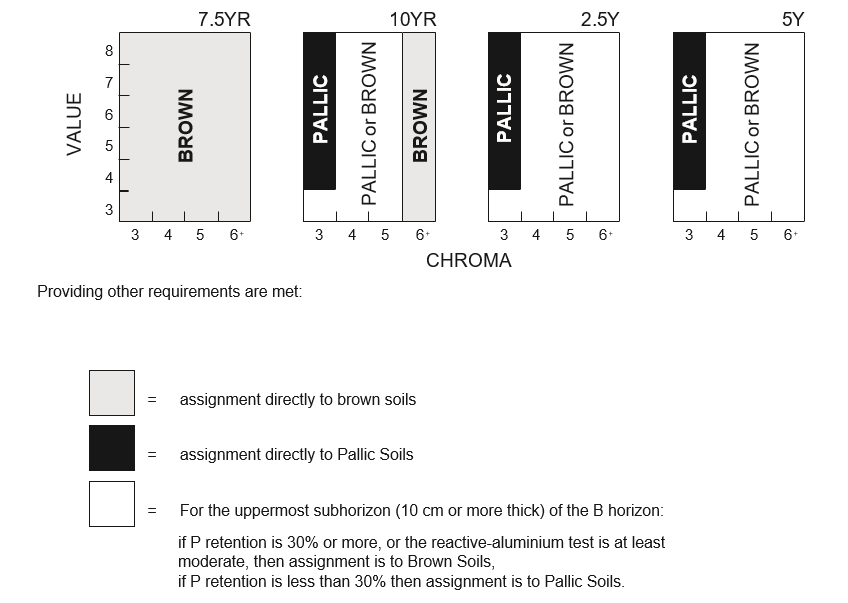
\includegraphics[width=0.85\textwidth,height=\textheight]{./images/Figure-002_pallic-vs-brown-colours_alternate-version.png}

}

\caption{\label{fig-2}Colour criteria, and colours where P retention and
the reactive-aluminium test is used to differentiate
\protect\hyperlink{sec-ord-B}{Brown Soils} from
\protect\hyperlink{sec-ord-P}{Pallic Soils} and
\protect\hyperlink{sec-ord-R}{Recent Soils}. See
\protect\hyperlink{sec-P}{part 2(a) of the Pallic Soils}, and
\protect\hyperlink{sec-B}{part 2(a) and 2(b) of the Brown Soils} in the
\protect\hyperlink{sec-key}{Key to Orders}.}

\end{figure}

\bookmarksetup{startatroot}

\hypertarget{sec-sec-ord-L}{%
\chapter{Allophanic Soils}\label{sec-sec-ord-L}}

\hypertarget{sec-sec-con-L}{%
\section{Concept of the Order}\label{sec-sec-con-L}}

Allophanic Soils have properties that are strongly influenced by
minerals with short-range order, especially allophane, imogolite and
ferrihydrite. They are characteristically weak in strength and
sensitive, with very low bulk density. They occur mostly in volcanic
parent materials, especially ash and basaltic scoria, but occur also in
quartzo-feldspathic and tuffaceous (greywacke) sandstone.

\hypertarget{sec-cor-L}{%
\section{Correlation}\label{sec-cor-L}}

The order comprises mainly yellow-brown loams but also includes weakly
weathered red loams and brown loams and some upland and high country
yellow-brown earths of the NZ Genetic Soil Classification. The soils
correlate predominantly with the Aquands, Cryands and Udands of Soil
Taxonomy.

\hypertarget{sec-occ-L}{%
\section{Occurrence}\label{sec-occ-L}}

Allophanic Soils occur predominantly in North Island volcanic ash, and
in the weathering products of other volcanic rocks. They also occur in
the weathering products of greywacke and schist in the South Island high
country.

\hypertarget{sec-acc-L}{%
\section{Accessory Properties of the Order}\label{sec-acc-L}}

\begin{enumerate}
\def\labelenumi{\arabic{enumi}.}
\tightlist
\item
  \emph{Short-range-order minerals.} The soil matrix as well as pore
  surfaces are dominated by the clay minerals allophane, imogolite and
  ferrihydrite, and/or aluminium-humus complexes. The soil materials
  have very high specific surface area. Measured clay contents generally
  range from 10 to 25\% though particle-size measurement is difficult
  because of aggregation and the ``true'' or primary clay contents may
  often be considerably higher. P retention is high or very high.
\item
  \emph{Low bases.} Sum of bases are low to very low and range from less
  than 1 to 10~cmol/100~g in subsoils and unfertilised topsoils.
\item
  \emph{Volcanic or greywacke parent materials.} Predominantly in
  andesitic, rhyolitic or mixed tephra, they also occur in soil
  materials from sandstone (greywacke) of humid uplands and high country
  and basalt scoria or pumice.
\item
  \emph{Rapidly weatherable minerals.} Volcanic glass and feldspar
  dominate the sand fractions of soils in igneous parent materials, and
  are the primary source of the short-range-order minerals. Feldspars
  are most likely the primary source in non-igneous parent materials.
  Typically they have an Amorphic mineralogy class.
\item
  \emph{Rapid permeability and high water retention.} The macroporosity
  is very high and rapid drainage occurs at low soil moisture tensions.
  Water contents at 1500~kPa soil moisture tension are very high.
\item
  \emph{Well drained.} Although poorly, imperfectly and moderately well
  drained soils occur, well drained soils are predominant.
\item
  \emph{Good rooting medium.} Bulk density is very low and there is
  little resistance to root extension. In many soils the potential
  rooting depth is very deep.
\item
  \emph{Active soil fauna.} Microbial biomass is generally high.
\item
  \emph{Stable topsoils.} Soils resist puddling under the impact of
  machinery or grazing animals in wet weather. The water content at
  field capacity is less than the plastic limit. Topsoil and subsoil
  horizons are friable, and organic/mineral complexes are stable. Carbon
  contents are medium to high. Exposed topsoil may be subject to wind
  erosion.
\item
  \emph{High shrinkage potential.} Soil materials have high potential to
  shrink on drying. Rewetting may not achieve the original volume.
\item
  \emph{Slight to insignificant erosion under pasture.} Generally the
  erosion potential is low, except on steep slopes or exposed sites and
  under cultivation on rolling slopes.
\item
  \emph{Sensitive.} A pronounced loss of strength occurs on disturbance.
\item
  \emph{Limited fertility.} There are usually requirements for
  phosphorus, potassium and magnesium on dairy farms. There are no
  significant trace element deficiencies although cobalt is marginal in
  more strongly leached Allophanic Soils. Pasture may respond to lime
  where pH is less than 5.3. Sulphate reserves are held in B horizons. P
  retention and phosphate fixation are high in topsoils.
\item
  \emph{Moist climate.} Precipitation exceeds 1000~mm and soil moisture
  deficits are either absent or occur for only short periods.
\end{enumerate}

\hypertarget{sec-sum-L}{%
\section{Summary of Allophanic Soils Hierarchy}\label{sec-sum-L}}

\begin{verbatim}
#> Warning: Warning: fonts used in `flextable` are ignored because the `pdflatex`
#> engine is used and not `xelatex` or `lualatex`. You can avoid this warning
#> by using the `set_flextable_defaults(fonts_ignore=TRUE)` command or use a
#> compatible engine by defining `latex_engine: xelatex` in the YAML header of the
#> R Markdown document.
\end{verbatim}

\providecommand{\docline}[3]{\noalign{\global\setlength{\arrayrulewidth}{#1}}\arrayrulecolor[HTML]{#2}\cline{#3}}

\setlength{\tabcolsep}{2pt}

\renewcommand*{\arraystretch}{1.5}

\begin{longtable}[c]{cccc}



\hhline{>{\arrayrulecolor[HTML]{666666}\global\arrayrulewidth=2pt}->{\arrayrulecolor[HTML]{666666}\global\arrayrulewidth=2pt}->{\arrayrulecolor[HTML]{666666}\global\arrayrulewidth=2pt}->{\arrayrulecolor[HTML]{666666}\global\arrayrulewidth=2pt}-}

\multicolumn{1}{!{\color[HTML]{000000}\vrule width 0pt}>{}l}{\fontsize{11}{11}\selectfont{\textcolor[HTML]{000000}{\textbf{Code}}}} & \multicolumn{1}{!{\color[HTML]{000000}\vrule width 0pt}>{}l}{\fontsize{11}{11}\selectfont{\textcolor[HTML]{000000}{\textbf{Group}}}} & \multicolumn{1}{!{\color[HTML]{000000}\vrule width 0pt}>{}l}{\fontsize{11}{11}\selectfont{\textcolor[HTML]{000000}{\textbf{Subgroup}}}} & \multicolumn{1}{!{\color[HTML]{000000}\vrule width 0pt}>{}l!{\color[HTML]{000000}\vrule width 0pt}}{\fontsize{11}{11}\selectfont{\textcolor[HTML]{000000}{\textbf{Example\ Series}}}} \\

\hhline{>{\arrayrulecolor[HTML]{666666}\global\arrayrulewidth=2pt}->{\arrayrulecolor[HTML]{666666}\global\arrayrulewidth=2pt}->{\arrayrulecolor[HTML]{666666}\global\arrayrulewidth=2pt}->{\arrayrulecolor[HTML]{666666}\global\arrayrulewidth=2pt}-}

\endfirsthead

\hhline{>{\arrayrulecolor[HTML]{666666}\global\arrayrulewidth=2pt}->{\arrayrulecolor[HTML]{666666}\global\arrayrulewidth=2pt}->{\arrayrulecolor[HTML]{666666}\global\arrayrulewidth=2pt}->{\arrayrulecolor[HTML]{666666}\global\arrayrulewidth=2pt}-}

\multicolumn{1}{!{\color[HTML]{000000}\vrule width 0pt}>{}l}{\fontsize{11}{11}\selectfont{\textcolor[HTML]{000000}{\textbf{Code}}}} & \multicolumn{1}{!{\color[HTML]{000000}\vrule width 0pt}>{}l}{\fontsize{11}{11}\selectfont{\textcolor[HTML]{000000}{\textbf{Group}}}} & \multicolumn{1}{!{\color[HTML]{000000}\vrule width 0pt}>{}l}{\fontsize{11}{11}\selectfont{\textcolor[HTML]{000000}{\textbf{Subgroup}}}} & \multicolumn{1}{!{\color[HTML]{000000}\vrule width 0pt}>{}l!{\color[HTML]{000000}\vrule width 0pt}}{\fontsize{11}{11}\selectfont{\textcolor[HTML]{000000}{\textbf{Example\ Series}}}} \\

\hhline{>{\arrayrulecolor[HTML]{666666}\global\arrayrulewidth=2pt}->{\arrayrulecolor[HTML]{666666}\global\arrayrulewidth=2pt}->{\arrayrulecolor[HTML]{666666}\global\arrayrulewidth=2pt}->{\arrayrulecolor[HTML]{666666}\global\arrayrulewidth=2pt}-}\endhead



\multicolumn{1}{!{\color[HTML]{000000}\vrule width 0pt}>{}l}{} & \multicolumn{1}{!{\color[HTML]{000000}\vrule width 0pt}>{}l}{} & \multicolumn{1}{!{\color[HTML]{000000}\vrule width 0pt}>{}l}{\fontsize{11}{11}\selectfont{\textcolor[HTML]{000000}{Ironstone}}} & \multicolumn{1}{!{\color[HTML]{000000}\vrule width 0pt}>{}l!{\color[HTML]{000000}\vrule width 0pt}}{\fontsize{11}{11}\selectfont{\textcolor[HTML]{000000}{-}}} \\





\multicolumn{1}{!{\color[HTML]{000000}\vrule width 0pt}>{}l}{\multirow[t]{-2}{*}{\parbox{0.75in}{\fontsize{11}{11}\selectfont{\textcolor[HTML]{000000}{\textbf{LP}}}}}} & \multicolumn{1}{!{\color[HTML]{000000}\vrule width 0pt}>{}l}{\multirow[t]{-2}{*}{\parbox{0.75in}{\fontsize{11}{11}\selectfont{\textcolor[HTML]{000000}{Perch-gley}}}}} & \multicolumn{1}{!{\color[HTML]{000000}\vrule width 0pt}>{}l}{\fontsize{11}{11}\selectfont{\textcolor[HTML]{000000}{Typic}}} & \multicolumn{1}{!{\color[HTML]{000000}\vrule width 0pt}>{}l!{\color[HTML]{000000}\vrule width 0pt}}{\fontsize{11}{11}\selectfont{\textcolor[HTML]{000000}{\href{https://viewer-nsdr.landcareresearch.co.nz/soil/id/nsdr/sa\_site/1854?view=sitereport}{Awatuna}}}} \\





\multicolumn{1}{!{\color[HTML]{000000}\vrule width 0pt}>{}l}{} & \multicolumn{1}{!{\color[HTML]{000000}\vrule width 0pt}>{}l}{} & \multicolumn{1}{!{\color[HTML]{000000}\vrule width 0pt}>{}l}{\fontsize{11}{11}\selectfont{\textcolor[HTML]{000000}{Peaty}}} & \multicolumn{1}{!{\color[HTML]{000000}\vrule width 0pt}>{}l!{\color[HTML]{000000}\vrule width 0pt}}{\fontsize{11}{11}\selectfont{\textcolor[HTML]{000000}{Rahotu\ var.}}} \\





\multicolumn{1}{!{\color[HTML]{000000}\vrule width 0pt}>{}l}{\multirow[t]{-2}{*}{\parbox{0.75in}{\fontsize{11}{11}\selectfont{\textcolor[HTML]{000000}{\textbf{LG}}}}}} & \multicolumn{1}{!{\color[HTML]{000000}\vrule width 0pt}>{}l}{\multirow[t]{-2}{*}{\parbox{0.75in}{\fontsize{11}{11}\selectfont{\textcolor[HTML]{000000}{Gley}}}}} & \multicolumn{1}{!{\color[HTML]{000000}\vrule width 0pt}>{}l}{\fontsize{11}{11}\selectfont{\textcolor[HTML]{000000}{Typic}}} & \multicolumn{1}{!{\color[HTML]{000000}\vrule width 0pt}>{}l!{\color[HTML]{000000}\vrule width 0pt}}{\fontsize{11}{11}\selectfont{\textcolor[HTML]{000000}{\href{https://viewer-nsdr.landcareresearch.co.nz/soil/id/nsdr/sa\_site/2766?view=sitereport}{Glenn}}}} \\





\multicolumn{1}{!{\color[HTML]{000000}\vrule width 0pt}>{}l}{} & \multicolumn{1}{!{\color[HTML]{000000}\vrule width 0pt}>{}l}{} & \multicolumn{1}{!{\color[HTML]{000000}\vrule width 0pt}>{}l}{\fontsize{11}{11}\selectfont{\textcolor[HTML]{000000}{Mottled-Ironstone}}} & \multicolumn{1}{!{\color[HTML]{000000}\vrule width 0pt}>{}l!{\color[HTML]{000000}\vrule width 0pt}}{\fontsize{11}{11}\selectfont{\textcolor[HTML]{000000}{pt.\ Okato\ var.}}} \\





\multicolumn{1}{!{\color[HTML]{000000}\vrule width 0pt}>{}l}{} & \multicolumn{1}{!{\color[HTML]{000000}\vrule width 0pt}>{}l}{} & \multicolumn{1}{!{\color[HTML]{000000}\vrule width 0pt}>{}l}{\fontsize{11}{11}\selectfont{\textcolor[HTML]{000000}{Mottled}}} & \multicolumn{1}{!{\color[HTML]{000000}\vrule width 0pt}>{}l!{\color[HTML]{000000}\vrule width 0pt}}{\fontsize{11}{11}\selectfont{\textcolor[HTML]{000000}{\href{https://viewer-nsdr.landcareresearch.co.nz/soil/id/nsdr/sa\_site/1597?view=sitereport}{Tipoka}}}} \\





\multicolumn{1}{!{\color[HTML]{000000}\vrule width 0pt}>{}l}{\multirow[t]{-3}{*}{\parbox{0.75in}{\fontsize{11}{11}\selectfont{\textcolor[HTML]{000000}{\textbf{LI}}}}}} & \multicolumn{1}{!{\color[HTML]{000000}\vrule width 0pt}>{}l}{\multirow[t]{-3}{*}{\parbox{0.75in}{\fontsize{11}{11}\selectfont{\textcolor[HTML]{000000}{Impeded}}}}} & \multicolumn{1}{!{\color[HTML]{000000}\vrule width 0pt}>{}l}{\fontsize{11}{11}\selectfont{\textcolor[HTML]{000000}{Typic}}} & \multicolumn{1}{!{\color[HTML]{000000}\vrule width 0pt}>{}l!{\color[HTML]{000000}\vrule width 0pt}}{\fontsize{11}{11}\selectfont{\textcolor[HTML]{000000}{\href{https://viewer-nsdr.landcareresearch.co.nz/soil/id/nsdr/sa\_site/2763?view=sitereport}{Bruntwood}}}} \\





\multicolumn{1}{!{\color[HTML]{000000}\vrule width 0pt}>{}l}{} & \multicolumn{1}{!{\color[HTML]{000000}\vrule width 0pt}>{}l}{} & \multicolumn{1}{!{\color[HTML]{000000}\vrule width 0pt}>{}l}{\fontsize{11}{11}\selectfont{\textcolor[HTML]{000000}{Mottled}}} & \multicolumn{1}{!{\color[HTML]{000000}\vrule width 0pt}>{}l!{\color[HTML]{000000}\vrule width 0pt}}{\fontsize{11}{11}\selectfont{\textcolor[HTML]{000000}{\href{https://viewer-nsdr.landcareresearch.co.nz/soil/id/nsdr/sa\_site/2786?view=sitereport}{Oeo}}}} \\





\multicolumn{1}{!{\color[HTML]{000000}\vrule width 0pt}>{}l}{} & \multicolumn{1}{!{\color[HTML]{000000}\vrule width 0pt}>{}l}{} & \multicolumn{1}{!{\color[HTML]{000000}\vrule width 0pt}>{}l}{\fontsize{11}{11}\selectfont{\textcolor[HTML]{000000}{Vitric-Acidic}}} & \multicolumn{1}{!{\color[HTML]{000000}\vrule width 0pt}>{}l!{\color[HTML]{000000}\vrule width 0pt}}{\fontsize{11}{11}\selectfont{\textcolor[HTML]{000000}{\href{https://viewer-nsdr.landcareresearch.co.nz/soil/id/nsdr/sa\_site/1742?view=sitereport}{Rowan}}}} \\





\multicolumn{1}{!{\color[HTML]{000000}\vrule width 0pt}>{}l}{} & \multicolumn{1}{!{\color[HTML]{000000}\vrule width 0pt}>{}l}{} & \multicolumn{1}{!{\color[HTML]{000000}\vrule width 0pt}>{}l}{\fontsize{11}{11}\selectfont{\textcolor[HTML]{000000}{Vitric}}} & \multicolumn{1}{!{\color[HTML]{000000}\vrule width 0pt}>{}l!{\color[HTML]{000000}\vrule width 0pt}}{\fontsize{11}{11}\selectfont{\textcolor[HTML]{000000}{\href{https://viewer-nsdr.landcareresearch.co.nz/soil/id/nsdr/sa\_site/1937?view=sitereport}{Lepperton}}}} \\





\multicolumn{1}{!{\color[HTML]{000000}\vrule width 0pt}>{}l}{} & \multicolumn{1}{!{\color[HTML]{000000}\vrule width 0pt}>{}l}{} & \multicolumn{1}{!{\color[HTML]{000000}\vrule width 0pt}>{}l}{\fontsize{11}{11}\selectfont{\textcolor[HTML]{000000}{Acidic}}} & \multicolumn{1}{!{\color[HTML]{000000}\vrule width 0pt}>{}l!{\color[HTML]{000000}\vrule width 0pt}}{\fontsize{11}{11}\selectfont{\textcolor[HTML]{000000}{\href{https://viewer-nsdr.landcareresearch.co.nz/soil/id/nsdr/sa\_site/1940?view=sitereport}{Patua}}}} \\





\multicolumn{1}{!{\color[HTML]{000000}\vrule width 0pt}>{}l}{\multirow[t]{-5}{*}{\parbox{0.75in}{\fontsize{11}{11}\selectfont{\textcolor[HTML]{000000}{\textbf{LO}}}}}} & \multicolumn{1}{!{\color[HTML]{000000}\vrule width 0pt}>{}l}{\multirow[t]{-5}{*}{\parbox{0.75in}{\fontsize{11}{11}\selectfont{\textcolor[HTML]{000000}{Orthic}}}}} & \multicolumn{1}{!{\color[HTML]{000000}\vrule width 0pt}>{}l}{\fontsize{11}{11}\selectfont{\textcolor[HTML]{000000}{Typic}}} & \multicolumn{1}{!{\color[HTML]{000000}\vrule width 0pt}>{}l!{\color[HTML]{000000}\vrule width 0pt}}{\fontsize{11}{11}\selectfont{\textcolor[HTML]{000000}{\href{https://viewer-nsdr.landcareresearch.co.nz/soil/id/nsdr/sa\_site/2964?view=sitereport}{Tirau}}}} \\

\hhline{>{\arrayrulecolor[HTML]{666666}\global\arrayrulewidth=2pt}->{\arrayrulecolor[HTML]{666666}\global\arrayrulewidth=2pt}->{\arrayrulecolor[HTML]{666666}\global\arrayrulewidth=2pt}->{\arrayrulecolor[HTML]{666666}\global\arrayrulewidth=2pt}-}



\end{longtable}

\begin{center}\rule{0.5\linewidth}{0.5pt}\end{center}

\hypertarget{sec-grp-L}{%
\section{Key to Groups of Allophanic Soils}\label{sec-grp-L}}

\hypertarget{sec-key-LP}{%
\subsubsection{\texorpdfstring{\textbf{LP}}{LP}}\label{sec-key-LP}}

Allophanic Soils that have both

\begin{enumerate}
\def\labelenumi{\arabic{enumi}.}
\tightlist
\item
  \protect\hyperlink{sec-sec-diag-pgley}{Perch-gley features},
  \emph{and}
\item
  Either a \protect\hyperlink{sec-diag-pts}{peaty topsoil}, or within
  15~cm of the base of the A horizon or 30~cm of the mineral soil
  surface, have

  \begin{enumerate}
  \def\labelenumii{(\alph{enumii})}
  \tightlist
  \item
    a \protect\hyperlink{sec-diag-redmh}{reductimorphic horizon},
    \emph{or}
  \item
    a \protect\hyperlink{sec-diag-roxh}{redox-mottled horizon} if the
    parent material is predominantly andesitic or basaltic.
  \end{enumerate}
\end{enumerate}

\protect\hyperlink{sec-LP}{\textbf{PERCH-GLEY ALLOPHANIC SOILS}}

\hypertarget{sec-key-LG}{%
\subsubsection{\texorpdfstring{\textbf{LG}}{LG}}\label{sec-key-LG}}

Other Allophanic Soils that have a
\protect\hyperlink{sec-diag-pts}{peaty topsoil}, or within 15~cm of the
base of the A horizon or 30~cm of the mineral soil surface, have either

\begin{enumerate}
\def\labelenumi{\arabic{enumi}.}
\tightlist
\item
  a \protect\hyperlink{sec-diag-redmh}{reductimorphic horizon},
  \textbf{\emph{or}}
\item
  a \protect\hyperlink{sec-diag-roxh}{redox-mottled horizon} if the
  parent material is predominantly andesitic or basaltic.
\end{enumerate}

\protect\hyperlink{sec-LG}{\textbf{GLEY ALLOPHANIC SOILS}}

\hypertarget{sec-key-LI}{%
\subsubsection{\texorpdfstring{\textbf{LI}}{LI}}\label{sec-key-LI}}

Other Allophanic Soils that have a
\protect\hyperlink{sec-diag-slowp}{slowly permeable layer}, or horizon
that is at least weakly indurated, within 90~cm of the mineral soil
surface.

\protect\hyperlink{sec-LI}{\textbf{IMPEDED ALLOPHANIC SOILS}}

\hypertarget{sec-key-LO}{%
\subsubsection{\texorpdfstring{\textbf{LO}}{LO}}\label{sec-key-LO}}

Other Allophanic Soils.

\protect\hyperlink{sec-LO}{\textbf{ORTHIC ALLOPHANIC SOILS}}

\begin{center}\rule{0.5\linewidth}{0.5pt}\end{center}

\hypertarget{sec-sub-L}{%
\section{Key to Subgroups of Allophanic Soils}\label{sec-sub-L}}

\hypertarget{sec-LP}{%
\subsection{\texorpdfstring{\textbf{LP} - PERCH-GLEY ALLOPHANIC
SOILS}{LP - PERCH-GLEY ALLOPHANIC SOILS}}\label{sec-LP}}

Perch-gley Allophanic Soils occur in sites that are periodically
saturated (unless artificially drained). Wetness and associated reducing
conditions are indicated by brownish or reddish mottles. The wetness is
caused by the perching of water on a slowly permeable subsurface layer,
although a groundwater-table may also be present.

\hypertarget{sec-key-LPI}{%
\subsubsection{\texorpdfstring{\textbf{LPI}}{LPI}}\label{sec-key-LPI}}

Perch-gley Allophanic Soils that have an
\protect\hyperlink{sec-diag-ipan}{ironstone-pan} within 90~cm of the
mineral soil surface.

\textbf{Ironstone Perch-gley Allophanic Soils}

\hypertarget{sec-key-LPT}{%
\subsubsection{\texorpdfstring{\textbf{LPT}}{LPT}}\label{sec-key-LPT}}

Other soils.

\textbf{Typic Perch-gley Allophanic Soils}

\hypertarget{sec-LG}{%
\subsection{\texorpdfstring{\textbf{LG} - GLEY ALLOPHANIC
SOILS}{LG - GLEY ALLOPHANIC SOILS}}\label{sec-LG}}

Gley Allophanic Soils occur in sites that are periodically saturated
(unless artificially drained). Wetness and associated reducing
conditions are indicated by brownish or reddish mottles. The wetness is
caused by a groundwater-table.

\hypertarget{sec-key-LGO}{%
\subsubsection{\texorpdfstring{\textbf{LGO}}{LGO}}\label{sec-key-LGO}}

Gley Allophanic Soils that have a \protect\hyperlink{sec-diag-pts}{peaty
topsoil}.

\textbf{Peaty Gley Allophanic Soils}

\hypertarget{sec-key-LGT}{%
\subsubsection{\texorpdfstring{\textbf{LGT}}{LGT}}\label{sec-key-LGT}}

Other soils.

\textbf{Typic Gley Allophanic Soils}

\hypertarget{sec-LI}{%
\subsection{\texorpdfstring{\textbf{LI} - IMPEDED ALLOPHANIC
SOILS}{LI - IMPEDED ALLOPHANIC SOILS}}\label{sec-LI}}

Impeded Allophanic Soils have a subsurface horizon that acts as a
barrier to the movement of water or penetration of roots.

\hypertarget{sec-key-LIMI}{%
\subsubsection{\texorpdfstring{\textbf{LIMI}}{LIMI}}\label{sec-key-LIMI}}

Impeded Allophanic Soils that have an ironstone-pan within 90~cm of the
mineral soil surface and that have a
\protect\hyperlink{sec-diag-mottpf}{mottled profile form}.

\textbf{Mottled-ironstone Impeded Allophanic Soils}

\hypertarget{sec-key-LIM}{%
\subsubsection{\texorpdfstring{\textbf{LIM}}{LIM}}\label{sec-key-LIM}}

Other soils that have a \protect\hyperlink{sec-diag-mottpf}{mottled
profile form}.

\textbf{Mottled Impeded Allophanic Soils}

\hypertarget{sec-key-LIT}{%
\subsubsection{\texorpdfstring{\textbf{LIT}}{LIT}}\label{sec-key-LIT}}

Other soils.

\textbf{Typic Impeded Allophanic Soils}

\hypertarget{sec-LO}{%
\subsection{\texorpdfstring{\textbf{LO} - ORTHIC ALLOPHANIC
SOILS}{LO - ORTHIC ALLOPHANIC SOILS}}\label{sec-LO}}

Orthic Allophanic Soils are permeable soils without barriers to deep
penetration of roots. They are moderately well, well or imperfectly
drained.

\hypertarget{sec-key-LOM}{%
\subsubsection{\texorpdfstring{\textbf{LOM}}{LOM}}\label{sec-key-LOM}}

Orthic Allophanic Soils that have a
\protect\hyperlink{sec-diag-mottpf}{mottled profile form}.

\textbf{Mottled Orthic Allophanic Soils}

\hypertarget{sec-key-LOVA}{%
\subsubsection{\texorpdfstring{\textbf{LOVA}}{LOVA}}\label{sec-key-LOVA}}

Other soils that have both 1. \textbf{\emph{either}} (a) coatings on
pores (excluding root linings), or gel-like masses bridging sand grains
or coating coarse-fragments, that have hue 7.5YR or redder, value 5 or
less and chroma 3 or more, \emph{or} (b) pH less than 5.5 in some part
of the B horizon to 60~cm from the mineral soil surface, \emph{and} 2.
\protect\hyperlink{sec-diag-alloph}{allophanic soil material} that is
formed predominantly from \protect\hyperlink{sec-diag-teph}{tephric soil
material} and has 50\% or more sand (by weighted average).

\textbf{Vitric-acidic Orthic Allophanic Soils}

\hypertarget{sec-key-LOV}{%
\subsubsection{\texorpdfstring{\textbf{LOV}}{LOV}}\label{sec-key-LOV}}

Other soils in which \protect\hyperlink{sec-diag-alloph}{allophanic soil
material} layers are formed predominantly from
\protect\hyperlink{sec-diag-teph}{tephric soil material} and have 50\%
or more sand (by weighted average).

\textbf{Vitric Orthic Allophanic Soils}

\hypertarget{sec-key-LOA}{%
\subsubsection{\texorpdfstring{\textbf{LOA}}{LOA}}\label{sec-key-LOA}}

Other soils that have, in some part of the B horizon to 60~cm from the
mineral soil surface, \emph{either}

\begin{enumerate}
\def\labelenumi{\arabic{enumi}.}
\tightlist
\item
  coatings on pores (excluding root linings), or gel-like masses
  bridging sand grains or coating coarse-fragments, that have hue 7.5YR
  or redder, value 5 or less and chroma 3 or more, \emph{or}
\item
  pH less than 5.5 in some part of the B horizon to 60~cm from the
  mineral soil surface.
\end{enumerate}

\textbf{Acidic Orthic Allophanic Soils}

\hypertarget{sec-key-LOT}{%
\subsubsection{\texorpdfstring{\textbf{LOT}}{LOT}}\label{sec-key-LOT}}

Other soils.

\textbf{Typic Orthic Allophanic Soils}

\bookmarksetup{startatroot}

\hypertarget{sec-ord-A}{%
\chapter{Anthropic Soils}\label{sec-ord-A}}

\hypertarget{sec-con-A}{%
\section{Concept of the Order}\label{sec-con-A}}

Anthropic Soils are soils that have been made by the direct action of
people, including truncation of natural soils by earth-moving equipment,
drastic mixing of natural soils so that their original character is
lost, or by deposition of thick layers of organic or inorganic material.
Anthropic Soils occur in land surfaces that are made by people. Their
classification reflects the way in which they were made and the kinds of
materials used.

Note that soils that have been drastically disturbed but have been
restored to the extent that they will meet the requirements of orders
other than \protect\hyperlink{sec-R}{Recent Soils} or
\protect\hyperlink{sec-W}{Raw Soils}, will not be assigned to Anthropic
Soils. For this reason Anthropic soils are placed late in the
\protect\hyperlink{sec-key}{Key to Orders} but before Recent Soils and
Raw Soils.

\hypertarget{sec-cor-A}{%
\section{Correlation}\label{sec-cor-A}}

Anthropic Soils were not formally part of the NZ Genetic Soil
Classification although anthropic soils were described in some soil
survey reports. The soils either correlate with Entisols or are
unclassified in Soil Taxonomy.

\hypertarget{sec-occ-A}{%
\section{Occurrence}\label{sec-occ-A}}

Anthropic Soils are most extensive in urban areas and areas that have
been mined.

\hypertarget{sec-acc-A}{%
\section{Accessory Properties of the Order}\label{sec-acc-A}}

\begin{enumerate}
\def\labelenumi{\arabic{enumi}.}
\tightlist
\item
  Soil characteristics and the relationships between soils and landforms
  do not have the orderliness of natural soils.
\item
  Drainage has often been changed significantly from the original state.
\item
  Soil properties depend upon both the nature of the manufactured or
  natural materials and the nature of the soil manipulation.
\item
  Land surfaces are artificial.
\end{enumerate}

\hypertarget{sec-sum-A}{%
\section{Summary of Anthropic Soils Hierarchy}\label{sec-sum-A}}

\begin{verbatim}
#> Warning: Warning: fonts used in `flextable` are ignored because the `pdflatex`
#> engine is used and not `xelatex` or `lualatex`. You can avoid this warning
#> by using the `set_flextable_defaults(fonts_ignore=TRUE)` command or use a
#> compatible engine by defining `latex_engine: xelatex` in the YAML header of the
#> R Markdown document.
\end{verbatim}

\providecommand{\docline}[3]{\noalign{\global\setlength{\arrayrulewidth}{#1}}\arrayrulecolor[HTML]{#2}\cline{#3}}

\setlength{\tabcolsep}{2pt}

\renewcommand*{\arraystretch}{1.5}

\begin{longtable}[c]{ccc}



\hhline{>{\arrayrulecolor[HTML]{666666}\global\arrayrulewidth=2pt}->{\arrayrulecolor[HTML]{666666}\global\arrayrulewidth=2pt}->{\arrayrulecolor[HTML]{666666}\global\arrayrulewidth=2pt}-}

\multicolumn{1}{!{\color[HTML]{000000}\vrule width 0pt}>{}l}{\fontsize{11}{11}\selectfont{\textcolor[HTML]{000000}{\textbf{Code}}}} & \multicolumn{1}{!{\color[HTML]{000000}\vrule width 0pt}>{}l}{\fontsize{11}{11}\selectfont{\textcolor[HTML]{000000}{\textbf{Group}}}} & \multicolumn{1}{!{\color[HTML]{000000}\vrule width 0pt}>{}l!{\color[HTML]{000000}\vrule width 0pt}}{\fontsize{11}{11}\selectfont{\textcolor[HTML]{000000}{\textbf{Subgroup}}}} \\

\hhline{>{\arrayrulecolor[HTML]{666666}\global\arrayrulewidth=2pt}->{\arrayrulecolor[HTML]{666666}\global\arrayrulewidth=2pt}->{\arrayrulecolor[HTML]{666666}\global\arrayrulewidth=2pt}-}

\endfirsthead

\hhline{>{\arrayrulecolor[HTML]{666666}\global\arrayrulewidth=2pt}->{\arrayrulecolor[HTML]{666666}\global\arrayrulewidth=2pt}->{\arrayrulecolor[HTML]{666666}\global\arrayrulewidth=2pt}-}

\multicolumn{1}{!{\color[HTML]{000000}\vrule width 0pt}>{}l}{\fontsize{11}{11}\selectfont{\textcolor[HTML]{000000}{\textbf{Code}}}} & \multicolumn{1}{!{\color[HTML]{000000}\vrule width 0pt}>{}l}{\fontsize{11}{11}\selectfont{\textcolor[HTML]{000000}{\textbf{Group}}}} & \multicolumn{1}{!{\color[HTML]{000000}\vrule width 0pt}>{}l!{\color[HTML]{000000}\vrule width 0pt}}{\fontsize{11}{11}\selectfont{\textcolor[HTML]{000000}{\textbf{Subgroup}}}} \\

\hhline{>{\arrayrulecolor[HTML]{666666}\global\arrayrulewidth=2pt}->{\arrayrulecolor[HTML]{666666}\global\arrayrulewidth=2pt}->{\arrayrulecolor[HTML]{666666}\global\arrayrulewidth=2pt}-}\endhead



\multicolumn{1}{!{\color[HTML]{000000}\vrule width 0pt}>{}l}{} & \multicolumn{1}{!{\color[HTML]{000000}\vrule width 0pt}>{}l}{} & \multicolumn{1}{!{\color[HTML]{000000}\vrule width 0pt}>{}l!{\color[HTML]{000000}\vrule width 0pt}}{\fontsize{11}{11}\selectfont{\textcolor[HTML]{000000}{Rocky}}} \\





\multicolumn{1}{!{\color[HTML]{000000}\vrule width 0pt}>{}l}{\multirow[t]{-2}{*}{\parbox{0.75in}{\fontsize{11}{11}\selectfont{\textcolor[HTML]{000000}{\textbf{AT}}}}}} & \multicolumn{1}{!{\color[HTML]{000000}\vrule width 0pt}>{}l}{\multirow[t]{-2}{*}{\parbox{0.75in}{\fontsize{11}{11}\selectfont{\textcolor[HTML]{000000}{Truncated}}}}} & \multicolumn{1}{!{\color[HTML]{000000}\vrule width 0pt}>{}l!{\color[HTML]{000000}\vrule width 0pt}}{\fontsize{11}{11}\selectfont{\textcolor[HTML]{000000}{Typic}}} \\





\multicolumn{1}{!{\color[HTML]{000000}\vrule width 0pt}>{}l}{} & \multicolumn{1}{!{\color[HTML]{000000}\vrule width 0pt}>{}l}{} & \multicolumn{1}{!{\color[HTML]{000000}\vrule width 0pt}>{}l!{\color[HTML]{000000}\vrule width 0pt}}{\fontsize{11}{11}\selectfont{\textcolor[HTML]{000000}{Buried\ Typic}}} \\





\multicolumn{1}{!{\color[HTML]{000000}\vrule width 0pt}>{}l}{\multirow[t]{-2}{*}{\parbox{0.75in}{\fontsize{11}{11}\selectfont{\textcolor[HTML]{000000}{\textbf{AR}}}}}} & \multicolumn{1}{!{\color[HTML]{000000}\vrule width 0pt}>{}l}{\multirow[t]{-2}{*}{\parbox{0.75in}{\fontsize{11}{11}\selectfont{\textcolor[HTML]{000000}{Refuse}}}}} & \multicolumn{1}{!{\color[HTML]{000000}\vrule width 0pt}>{}l!{\color[HTML]{000000}\vrule width 0pt}}{\fontsize{11}{11}\selectfont{\textcolor[HTML]{000000}{-}}} \\





\multicolumn{1}{!{\color[HTML]{000000}\vrule width 0pt}>{}l}{\fontsize{11}{11}\selectfont{\textcolor[HTML]{000000}{\textbf{AM}}}} & \multicolumn{1}{!{\color[HTML]{000000}\vrule width 0pt}>{}l}{\fontsize{11}{11}\selectfont{\textcolor[HTML]{000000}{Mixed}}} & \multicolumn{1}{!{\color[HTML]{000000}\vrule width 0pt}>{}l!{\color[HTML]{000000}\vrule width 0pt}}{\fontsize{11}{11}\selectfont{\textcolor[HTML]{000000}{Compacted}}} \\





\multicolumn{1}{!{\color[HTML]{000000}\vrule width 0pt}>{}l}{} & \multicolumn{1}{!{\color[HTML]{000000}\vrule width 0pt}>{}l}{} & \multicolumn{1}{!{\color[HTML]{000000}\vrule width 0pt}>{}l!{\color[HTML]{000000}\vrule width 0pt}}{\fontsize{11}{11}\selectfont{\textcolor[HTML]{000000}{Wet}}} \\





\multicolumn{1}{!{\color[HTML]{000000}\vrule width 0pt}>{}l}{} & \multicolumn{1}{!{\color[HTML]{000000}\vrule width 0pt}>{}l}{} & \multicolumn{1}{!{\color[HTML]{000000}\vrule width 0pt}>{}l!{\color[HTML]{000000}\vrule width 0pt}}{\fontsize{11}{11}\selectfont{\textcolor[HTML]{000000}{Stony-Tailings}}} \\





\multicolumn{1}{!{\color[HTML]{000000}\vrule width 0pt}>{}l}{} & \multicolumn{1}{!{\color[HTML]{000000}\vrule width 0pt}>{}l}{} & \multicolumn{1}{!{\color[HTML]{000000}\vrule width 0pt}>{}l!{\color[HTML]{000000}\vrule width 0pt}}{\fontsize{11}{11}\selectfont{\textcolor[HTML]{000000}{Artifact}}} \\





\multicolumn{1}{!{\color[HTML]{000000}\vrule width 0pt}>{}l}{\multirow[t]{-4}{*}{\parbox{0.75in}{\fontsize{11}{11}\selectfont{\textcolor[HTML]{000000}{\textbf{AF}}}}}} & \multicolumn{1}{!{\color[HTML]{000000}\vrule width 0pt}>{}l}{\multirow[t]{-4}{*}{\parbox{0.75in}{\fontsize{11}{11}\selectfont{\textcolor[HTML]{000000}{Fill}}}}} & \multicolumn{1}{!{\color[HTML]{000000}\vrule width 0pt}>{}l!{\color[HTML]{000000}\vrule width 0pt}}{\fontsize{11}{11}\selectfont{\textcolor[HTML]{000000}{Earthy}}} \\

\hhline{>{\arrayrulecolor[HTML]{666666}\global\arrayrulewidth=2pt}->{\arrayrulecolor[HTML]{666666}\global\arrayrulewidth=2pt}->{\arrayrulecolor[HTML]{666666}\global\arrayrulewidth=2pt}-}



\end{longtable}

\hypertarget{sec-grp-A}{%
\section{Key to Groups of Anthropic Soils}\label{sec-grp-A}}

\hypertarget{sec-key-AT}{%
\subsubsection{\texorpdfstring{\textbf{AT}}{AT}}\label{sec-key-AT}}

Anthropic Soils in which natural \emph{in-situ} materials occur at or
within 30~cm of the soil surface, which result from truncation of the
solum of the original soil by the action of people.

\protect\hyperlink{sec-AT}{\textbf{TRUNCATED ANTHROPIC SOILS}}

\hypertarget{sec-key-AR}{%
\subsubsection{\texorpdfstring{\textbf{AR}}{AR}}\label{sec-key-AR}}

Other Anthropic Soils that have either

\begin{enumerate}
\def\labelenumi{\arabic{enumi}.}
\tightlist
\item
  a layer comprising natural organic waste, or manufactured organic
  material, that is at least 30~cm thick and has an upper boundary at
  the land surface or buried within 90~cm of the land surface, \emph{or}
\item
  has a methane content sufficient to be detected by odour, or if
  trapped, by ignition.
\end{enumerate}

\protect\hyperlink{sec-AR}{\textbf{REFUSE ANTHROPIC SOILS}}

\hypertarget{sec-key-AM}{%
\subsubsection{\texorpdfstring{\textbf{AM}}{AM}}\label{sec-key-AM}}

Other Anthropic Soils in which the original soil horizons have been
destroyed by deep ripping, deep subsoil lifting, or some similar
practice.

\protect\hyperlink{sec-AM}{\textbf{MIXED ANTHROPIC SOILS}}

\hypertarget{sec-key-AF}{%
\subsubsection{\texorpdfstring{\textbf{AF}}{AF}}\label{sec-key-AF}}

Other Anthropic Soils.

\protect\hyperlink{sec-AF}{\textbf{FILL ANTHROPIC SOILS}}

\hypertarget{sec-sub-A}{%
\section{Key to Subgroups of Anthropic Soils}\label{sec-sub-A}}

\hypertarget{sec-AT}{%
\subsection{\texorpdfstring{\textbf{AT} - TRUNCATED ANTHROPIC
SOILS}{AT - TRUNCATED ANTHROPIC SOILS}}\label{sec-AT}}

Truncated Anthropic Soils result from cutting away any existing soil, by
mechanical equipment, leaving material that would be recognised as a BC,
C or R horizon. The scalped surface maybe overlain by up to 29~cm of
soil, deposited for landscaping purposes.

\hypertarget{sec-key-ATX}{%
\subsubsection{\texorpdfstring{\textbf{ATX}}{ATX}}\label{sec-key-ATX}}

Soils with a lithic contact within 60~cm of the soil surface.

\textbf{Rocky Truncated Anthropic Soils}

\hypertarget{sec-key-ATT}{%
\subsubsection{\texorpdfstring{\textbf{ATT}}{ATT}}\label{sec-key-ATT}}

Other soils.

\textbf{Typic Truncated Anthropic Soils}

\hypertarget{sec-AR}{%
\subsection{\texorpdfstring{\textbf{AR} - REFUSE ANTHROPIC
SOILS}{AR - REFUSE ANTHROPIC SOILS}}\label{sec-AR}}

Refuse Anthropic Soils occur in sites where household, land management,
urban or industrial waste has been dumped and which have significant
organic matter, comprising vegetation, animal or manufactured material
such as plastics, paper or timber.

\hypertarget{sec-key-ARB}{%
\subsubsection{\texorpdfstring{\textbf{ARB}}{ARB}}\label{sec-key-ARB}}

Soils in which organic refuse is buried beneath an overburden of soil or
rock material greater than 30~cm thick.

\textbf{Buried Refuse Anthropic Soils}

\hypertarget{sec-key-ART}{%
\subsubsection{\texorpdfstring{\textbf{ART}}{ART}}\label{sec-key-ART}}

Other Soils.

\textbf{Typic Refuse Anthropic Soils}

\hypertarget{sec-AM}{%
\subsection{\texorpdfstring{\textbf{AM} - MIXED ANTHROPIC
SOILS}{AM - MIXED ANTHROPIC SOILS}}\label{sec-AM}}

Mixed Anthropic Soils occur in sites where the original soil has been
drastically disturbed by mechanical procedures such as deep ripping.

No subgroups are defined, but the original soil if known may be appended
to the name in parentheses, for example Mixed Anthropic Soils
(Perch-Gley Pallic Soils).

\hypertarget{sec-AF}{%
\subsection{\texorpdfstring{\textbf{AF} - FILL ANTHROPIC
SOILS}{AF - FILL ANTHROPIC SOILS}}\label{sec-AF}}

Fill Anthropic Soils result from the deposition of dominantly inorganic
material including soil, rock debris, dredged sediments or manufactured
material such as bricks, concrete, or metals.

\hypertarget{sec-key-AFC}{%
\subsubsection{\texorpdfstring{\textbf{AFC}}{AFC}}\label{sec-key-AFC}}

Soils that have been compacted and have a bulk density of
1.5~Mg/m\textsuperscript{3} or more.

\textbf{Compacted Fill Anthropic Soils}

\hypertarget{sec-key-FWT}{%
\subsubsection{\texorpdfstring{\textbf{AFW}}{AFW}}\label{sec-key-FWT}}

Other soils that are wet within 60~cm of the mineral soil surface at
some time of the year.

\textbf{Wet Fill Anthropic Soils}

\hypertarget{sec-key-AFST}{%
\subsubsection{\texorpdfstring{\textbf{AFST}}{AFST}}\label{sec-key-AFST}}

Other soils that have a gravel or bouldery layer more than 30~cm thick
in which there is insufficient fine-earth to fill more than half the
interstices between the gravel or boulder clasts, with an upper boundary
within 60~cm of the mineral soil surface.

\textbf{Stony-tailings Fill Anthropic Soils}

\hypertarget{sec-key-AFA}{%
\subsubsection{\texorpdfstring{\textbf{AFA}}{AFA}}\label{sec-key-AFA}}

Other soils showing evidence of pre-European additions of material.

\textbf{Artifact Fill Anthropic Soils}

\hypertarget{sec-key-AFE}{%
\subsubsection{\texorpdfstring{\textbf{AFE}}{AFE}}\label{sec-key-AFE}}

Other soils.

\textbf{Earthy Fill Anthropic Soils}

\bookmarksetup{startatroot}

\hypertarget{sec-ord-B}{%
\chapter{Brown Soils}\label{sec-ord-B}}

\hypertarget{sec-con-B}{%
\section{Concept of the Order}\label{sec-con-B}}

Brown Soils usually contain 2:1 clay minerals. Secondary iron oxides
tend to be evenly dispersed through the soil and give a yellowish brown
colour to the upper part of the B horizon. Base saturation values are
usually moderate to very low.

\hypertarget{sec-cor-B}{%
\section{Correlation}\label{sec-cor-B}}

The order comprises moderately and weakly weathered yellow-brown earths,
yellow-brown sands, southern brown-granular loams and clays, and
intergrades from yellow-brown earths to yellow-grey earths, podzols,
brown-granular soils, and recent soils, as well as associated steepland
soils of the NZ Genetic Soil Classification. The soils predominantly
correlate with the Dystrochrepts of Soil Taxonomy, except for some stony
and sandy soils which are Ustochrepts or Psamments.

\hypertarget{sec-occ-B}{%
\section{Occurrence}\label{sec-occ-B}}

Brown Soils occur in places in which summer dryness is uncommon and that
are not waterlogged in winter. They are the most extensive New Zealand
soils.

\hypertarget{sec-acc-B}{%
\section{Accessory Properties of the Order}\label{sec-acc-B}}

\begin{enumerate}
\def\labelenumi{\arabic{enumi}.}
\tightlist
\item
  \emph{Dispersed secondary oxides.} Secondary iron and aluminium oxides
  are dispersed throughout the soil mass. The soil is brunified
  (i.e.~iron and aluminium oxides form coatings around phyllosilicate
  clay particles and form bridges between these particles and humus). P
  retention is moderate to very high.
\item
  \emph{Low to moderate base saturation.} Base saturation values in
  subsoils are usually less than 50\%, and KCl-extractable aluminium
  levels are usually more than 1.5~cmol(+)/kg except where clay contents
  are relatively low.
\item
  \emph{Parent materials are mostly weakly weathered.}
  \protect\hyperlink{sec-BM}{Mafic Brown Soils} are derived from weakly
  weathered intermediate or basic igneous rocks (e.g.~phonolite and
  basalt). Other groups are derived dominantly from acid
  quartzo-feldspathic sedimentary rocks (schist and greywacke) or acid
  igneous rocks (e.g.~rhyolites and granites).The alteration status of
  gravel or hard rock substrates is usually fresh to moderately
  weathered and occasionally highly weathered.
\item
  \emph{Mica/illite and vermiculite are common clay minerals.} Profiles
  tend to be mineralogically uniform with depth. Brown soils cover a
  wide range of mineralogy classes. Mixed, Illitic, Vermiculitic and
  Clay-mineralic (involving vermiculite and mica-vermiculite) are
  common. Some \protect\hyperlink{sec-BA}{Allophanic Brown Soils} have
  an Amorphic mineralogy class.
\item
  \emph{Good Drainage.} No poorly drained or very poorly drained soils
  are included. Macroporosity is generally moderate (10--14\%) except in
  subsurface horizons of \protect\hyperlink{sec-BF}{Firm Brown Soils}.
\item
  \emph{Biologically active.} Except in soils that are limited by
  coldness or acidity, cast spheroidal peds are common in topsoils and
  C/N ratios are moderate to low. The roots of native plants penetrate
  deeply.
\item
  \emph{Relatively stable topsoils.} Aggregates are not readily
  dispersed.
\item
  \emph{Moist climate or low available-water capacity.} Most soils occur
  in areas with mean annual precipitation more than 1000~mm. Others have
  low available-water capacity (usually less than 75~mm as in some Stony
  Brown Soils and \protect\hyperlink{sec-BS}{Sandy Brown Soils}), or are
  in sites with low evapotranspiration.
\end{enumerate}

\hypertarget{sec-sum-B}{%
\section{Summary of Brown Soils Hierarchy}\label{sec-sum-B}}

\begin{verbatim}
#> Warning: Warning: fonts used in `flextable` are ignored because the `pdflatex`
#> engine is used and not `xelatex` or `lualatex`. You can avoid this warning
#> by using the `set_flextable_defaults(fonts_ignore=TRUE)` command or use a
#> compatible engine by defining `latex_engine: xelatex` in the YAML header of the
#> R Markdown document.
\end{verbatim}

\providecommand{\docline}[3]{\noalign{\global\setlength{\arrayrulewidth}{#1}}\arrayrulecolor[HTML]{#2}\cline{#3}}

\setlength{\tabcolsep}{2pt}

\renewcommand*{\arraystretch}{1.5}

\begin{longtable}[c]{cccc}



\hhline{>{\arrayrulecolor[HTML]{666666}\global\arrayrulewidth=2pt}->{\arrayrulecolor[HTML]{666666}\global\arrayrulewidth=2pt}->{\arrayrulecolor[HTML]{666666}\global\arrayrulewidth=2pt}->{\arrayrulecolor[HTML]{666666}\global\arrayrulewidth=2pt}-}

\multicolumn{1}{!{\color[HTML]{000000}\vrule width 0pt}>{}l}{\fontsize{11}{11}\selectfont{\textcolor[HTML]{000000}{\textbf{Code}}}} & \multicolumn{1}{!{\color[HTML]{000000}\vrule width 0pt}>{}l}{\fontsize{11}{11}\selectfont{\textcolor[HTML]{000000}{\textbf{Group}}}} & \multicolumn{1}{!{\color[HTML]{000000}\vrule width 0pt}>{}l}{\fontsize{11}{11}\selectfont{\textcolor[HTML]{000000}{\textbf{Subgroup}}}} & \multicolumn{1}{!{\color[HTML]{000000}\vrule width 0pt}>{}l!{\color[HTML]{000000}\vrule width 0pt}}{\fontsize{11}{11}\selectfont{\textcolor[HTML]{000000}{\textbf{Example\ Series}}}} \\

\hhline{>{\arrayrulecolor[HTML]{666666}\global\arrayrulewidth=2pt}->{\arrayrulecolor[HTML]{666666}\global\arrayrulewidth=2pt}->{\arrayrulecolor[HTML]{666666}\global\arrayrulewidth=2pt}->{\arrayrulecolor[HTML]{666666}\global\arrayrulewidth=2pt}-}

\endfirsthead

\hhline{>{\arrayrulecolor[HTML]{666666}\global\arrayrulewidth=2pt}->{\arrayrulecolor[HTML]{666666}\global\arrayrulewidth=2pt}->{\arrayrulecolor[HTML]{666666}\global\arrayrulewidth=2pt}->{\arrayrulecolor[HTML]{666666}\global\arrayrulewidth=2pt}-}

\multicolumn{1}{!{\color[HTML]{000000}\vrule width 0pt}>{}l}{\fontsize{11}{11}\selectfont{\textcolor[HTML]{000000}{\textbf{Code}}}} & \multicolumn{1}{!{\color[HTML]{000000}\vrule width 0pt}>{}l}{\fontsize{11}{11}\selectfont{\textcolor[HTML]{000000}{\textbf{Group}}}} & \multicolumn{1}{!{\color[HTML]{000000}\vrule width 0pt}>{}l}{\fontsize{11}{11}\selectfont{\textcolor[HTML]{000000}{\textbf{Subgroup}}}} & \multicolumn{1}{!{\color[HTML]{000000}\vrule width 0pt}>{}l!{\color[HTML]{000000}\vrule width 0pt}}{\fontsize{11}{11}\selectfont{\textcolor[HTML]{000000}{\textbf{Example\ Series}}}} \\

\hhline{>{\arrayrulecolor[HTML]{666666}\global\arrayrulewidth=2pt}->{\arrayrulecolor[HTML]{666666}\global\arrayrulewidth=2pt}->{\arrayrulecolor[HTML]{666666}\global\arrayrulewidth=2pt}->{\arrayrulecolor[HTML]{666666}\global\arrayrulewidth=2pt}-}\endhead



\multicolumn{1}{!{\color[HTML]{000000}\vrule width 0pt}>{}l}{} & \multicolumn{1}{!{\color[HTML]{000000}\vrule width 0pt}>{}l}{} & \multicolumn{1}{!{\color[HTML]{000000}\vrule width 0pt}>{}l}{\fontsize{11}{11}\selectfont{\textcolor[HTML]{000000}{Mottled}}} & \multicolumn{1}{!{\color[HTML]{000000}\vrule width 0pt}>{}l!{\color[HTML]{000000}\vrule width 0pt}}{\fontsize{11}{11}\selectfont{\textcolor[HTML]{000000}{-}}} \\





\multicolumn{1}{!{\color[HTML]{000000}\vrule width 0pt}>{}l}{} & \multicolumn{1}{!{\color[HTML]{000000}\vrule width 0pt}>{}l}{} & \multicolumn{1}{!{\color[HTML]{000000}\vrule width 0pt}>{}l}{\fontsize{11}{11}\selectfont{\textcolor[HTML]{000000}{Acidic}}} & \multicolumn{1}{!{\color[HTML]{000000}\vrule width 0pt}>{}l!{\color[HTML]{000000}\vrule width 0pt}}{\fontsize{11}{11}\selectfont{\textcolor[HTML]{000000}{Tekoa}}} \\





\multicolumn{1}{!{\color[HTML]{000000}\vrule width 0pt}>{}l}{} & \multicolumn{1}{!{\color[HTML]{000000}\vrule width 0pt}>{}l}{} & \multicolumn{1}{!{\color[HTML]{000000}\vrule width 0pt}>{}l}{\fontsize{11}{11}\selectfont{\textcolor[HTML]{000000}{Firm}}} & \multicolumn{1}{!{\color[HTML]{000000}\vrule width 0pt}>{}l!{\color[HTML]{000000}\vrule width 0pt}}{\fontsize{11}{11}\selectfont{\textcolor[HTML]{000000}{Te\ Anau}}} \\





\multicolumn{1}{!{\color[HTML]{000000}\vrule width 0pt}>{}l}{} & \multicolumn{1}{!{\color[HTML]{000000}\vrule width 0pt}>{}l}{} & \multicolumn{1}{!{\color[HTML]{000000}\vrule width 0pt}>{}l}{\fontsize{11}{11}\selectfont{\textcolor[HTML]{000000}{Acidic-mafic}}} & \multicolumn{1}{!{\color[HTML]{000000}\vrule width 0pt}>{}l!{\color[HTML]{000000}\vrule width 0pt}}{\fontsize{11}{11}\selectfont{\textcolor[HTML]{000000}{Stewart}}} \\





\multicolumn{1}{!{\color[HTML]{000000}\vrule width 0pt}>{}l}{} & \multicolumn{1}{!{\color[HTML]{000000}\vrule width 0pt}>{}l}{} & \multicolumn{1}{!{\color[HTML]{000000}\vrule width 0pt}>{}l}{\fontsize{11}{11}\selectfont{\textcolor[HTML]{000000}{Typic}}} & \multicolumn{1}{!{\color[HTML]{000000}\vrule width 0pt}>{}l!{\color[HTML]{000000}\vrule width 0pt}}{\fontsize{11}{11}\selectfont{\textcolor[HTML]{000000}{Craigieburn}}} \\





\multicolumn{1}{!{\color[HTML]{000000}\vrule width 0pt}>{}l}{} & \multicolumn{1}{!{\color[HTML]{000000}\vrule width 0pt}>{}l}{} & \multicolumn{1}{!{\color[HTML]{000000}\vrule width 0pt}>{}l}{\fontsize{11}{11}\selectfont{\textcolor[HTML]{000000}{Acidic-pedal}}} & \multicolumn{1}{!{\color[HTML]{000000}\vrule width 0pt}>{}l!{\color[HTML]{000000}\vrule width 0pt}}{\fontsize{11}{11}\selectfont{\textcolor[HTML]{000000}{Kaiuma}}} \\





\multicolumn{1}{!{\color[HTML]{000000}\vrule width 0pt}>{}l}{\multirow[t]{-7}{*}{\parbox{0.75in}{\fontsize{11}{11}\selectfont{\textcolor[HTML]{000000}{\textbf{BL}}}}}} & \multicolumn{1}{!{\color[HTML]{000000}\vrule width 0pt}>{}l}{\multirow[t]{-7}{*}{\parbox{0.75in}{\fontsize{11}{11}\selectfont{\textcolor[HTML]{000000}{Allophanic}}}}} & \multicolumn{1}{!{\color[HTML]{000000}\vrule width 0pt}>{}l}{\fontsize{11}{11}\selectfont{\textcolor[HTML]{000000}{Pedal}}} & \multicolumn{1}{!{\color[HTML]{000000}\vrule width 0pt}>{}l!{\color[HTML]{000000}\vrule width 0pt}}{\fontsize{11}{11}\selectfont{\textcolor[HTML]{000000}{Levin}}} \\





\multicolumn{1}{!{\color[HTML]{000000}\vrule width 0pt}>{}l}{} & \multicolumn{1}{!{\color[HTML]{000000}\vrule width 0pt}>{}l}{} & \multicolumn{1}{!{\color[HTML]{000000}\vrule width 0pt}>{}l}{\fontsize{11}{11}\selectfont{\textcolor[HTML]{000000}{Mottled-Placic}}} & \multicolumn{1}{!{\color[HTML]{000000}\vrule width 0pt}>{}l!{\color[HTML]{000000}\vrule width 0pt}}{\fontsize{11}{11}\selectfont{\textcolor[HTML]{000000}{-}}} \\





\multicolumn{1}{!{\color[HTML]{000000}\vrule width 0pt}>{}l}{} & \multicolumn{1}{!{\color[HTML]{000000}\vrule width 0pt}>{}l}{} & \multicolumn{1}{!{\color[HTML]{000000}\vrule width 0pt}>{}l}{\fontsize{11}{11}\selectfont{\textcolor[HTML]{000000}{Mottled}}} & \multicolumn{1}{!{\color[HTML]{000000}\vrule width 0pt}>{}l!{\color[HTML]{000000}\vrule width 0pt}}{\fontsize{11}{11}\selectfont{\textcolor[HTML]{000000}{Awahou}}} \\





\multicolumn{1}{!{\color[HTML]{000000}\vrule width 0pt}>{}l}{} & \multicolumn{1}{!{\color[HTML]{000000}\vrule width 0pt}>{}l}{} & \multicolumn{1}{!{\color[HTML]{000000}\vrule width 0pt}>{}l}{\fontsize{11}{11}\selectfont{\textcolor[HTML]{000000}{Acidic}}} & \multicolumn{1}{!{\color[HTML]{000000}\vrule width 0pt}>{}l!{\color[HTML]{000000}\vrule width 0pt}}{\fontsize{11}{11}\selectfont{\textcolor[HTML]{000000}{Koputaroa}}} \\





\multicolumn{1}{!{\color[HTML]{000000}\vrule width 0pt}>{}l}{} & \multicolumn{1}{!{\color[HTML]{000000}\vrule width 0pt}>{}l}{} & \multicolumn{1}{!{\color[HTML]{000000}\vrule width 0pt}>{}l}{\fontsize{11}{11}\selectfont{\textcolor[HTML]{000000}{Pallic}}} & \multicolumn{1}{!{\color[HTML]{000000}\vrule width 0pt}>{}l!{\color[HTML]{000000}\vrule width 0pt}}{\fontsize{11}{11}\selectfont{\textcolor[HTML]{000000}{pt.\ Halkett}}} \\





\multicolumn{1}{!{\color[HTML]{000000}\vrule width 0pt}>{}l}{} & \multicolumn{1}{!{\color[HTML]{000000}\vrule width 0pt}>{}l}{} & \multicolumn{1}{!{\color[HTML]{000000}\vrule width 0pt}>{}l}{\fontsize{11}{11}\selectfont{\textcolor[HTML]{000000}{Pan}}} & \multicolumn{1}{!{\color[HTML]{000000}\vrule width 0pt}>{}l!{\color[HTML]{000000}\vrule width 0pt}}{\fontsize{11}{11}\selectfont{\textcolor[HTML]{000000}{ToeToes}}} \\





\multicolumn{1}{!{\color[HTML]{000000}\vrule width 0pt}>{}l}{\multirow[t]{-6}{*}{\parbox{0.75in}{\fontsize{11}{11}\selectfont{\textcolor[HTML]{000000}{\textbf{BS}}}}}} & \multicolumn{1}{!{\color[HTML]{000000}\vrule width 0pt}>{}l}{\multirow[t]{-6}{*}{\parbox{0.75in}{\fontsize{11}{11}\selectfont{\textcolor[HTML]{000000}{Sandy}}}}} & \multicolumn{1}{!{\color[HTML]{000000}\vrule width 0pt}>{}l}{\fontsize{11}{11}\selectfont{\textcolor[HTML]{000000}{Typic}}} & \multicolumn{1}{!{\color[HTML]{000000}\vrule width 0pt}>{}l!{\color[HTML]{000000}\vrule width 0pt}}{\fontsize{11}{11}\selectfont{\textcolor[HTML]{000000}{Foxton}}} \\





\multicolumn{1}{!{\color[HTML]{000000}\vrule width 0pt}>{}l}{\fontsize{11}{11}\selectfont{\textcolor[HTML]{000000}{\textbf{BX}}}} & \multicolumn{1}{!{\color[HTML]{000000}\vrule width 0pt}>{}l}{\fontsize{11}{11}\selectfont{\textcolor[HTML]{000000}{Oxidic}}} & \multicolumn{1}{!{\color[HTML]{000000}\vrule width 0pt}>{}l}{\fontsize{11}{11}\selectfont{\textcolor[HTML]{000000}{Typic}}} & \multicolumn{1}{!{\color[HTML]{000000}\vrule width 0pt}>{}l!{\color[HTML]{000000}\vrule width 0pt}}{\fontsize{11}{11}\selectfont{\textcolor[HTML]{000000}{-}}} \\





\multicolumn{1}{!{\color[HTML]{000000}\vrule width 0pt}>{}l}{} & \multicolumn{1}{!{\color[HTML]{000000}\vrule width 0pt}>{}l}{} & \multicolumn{1}{!{\color[HTML]{000000}\vrule width 0pt}>{}l}{\fontsize{11}{11}\selectfont{\textcolor[HTML]{000000}{Mottled-magnesic}}} & \multicolumn{1}{!{\color[HTML]{000000}\vrule width 0pt}>{}l!{\color[HTML]{000000}\vrule width 0pt}}{\fontsize{11}{11}\selectfont{\textcolor[HTML]{000000}{Croisilles\ var.}}} \\





\multicolumn{1}{!{\color[HTML]{000000}\vrule width 0pt}>{}l}{} & \multicolumn{1}{!{\color[HTML]{000000}\vrule width 0pt}>{}l}{} & \multicolumn{1}{!{\color[HTML]{000000}\vrule width 0pt}>{}l}{\fontsize{11}{11}\selectfont{\textcolor[HTML]{000000}{Magnesic}}} & \multicolumn{1}{!{\color[HTML]{000000}\vrule width 0pt}>{}l!{\color[HTML]{000000}\vrule width 0pt}}{\fontsize{11}{11}\selectfont{\textcolor[HTML]{000000}{pt.\ Dun}}} \\





\multicolumn{1}{!{\color[HTML]{000000}\vrule width 0pt}>{}l}{} & \multicolumn{1}{!{\color[HTML]{000000}\vrule width 0pt}>{}l}{} & \multicolumn{1}{!{\color[HTML]{000000}\vrule width 0pt}>{}l}{\fontsize{11}{11}\selectfont{\textcolor[HTML]{000000}{Mottled}}} & \multicolumn{1}{!{\color[HTML]{000000}\vrule width 0pt}>{}l!{\color[HTML]{000000}\vrule width 0pt}}{\fontsize{11}{11}\selectfont{\textcolor[HTML]{000000}{-}}} \\





\multicolumn{1}{!{\color[HTML]{000000}\vrule width 0pt}>{}l}{} & \multicolumn{1}{!{\color[HTML]{000000}\vrule width 0pt}>{}l}{} & \multicolumn{1}{!{\color[HTML]{000000}\vrule width 0pt}>{}l}{\fontsize{11}{11}\selectfont{\textcolor[HTML]{000000}{Acidic}}} & \multicolumn{1}{!{\color[HTML]{000000}\vrule width 0pt}>{}l!{\color[HTML]{000000}\vrule width 0pt}}{\fontsize{11}{11}\selectfont{\textcolor[HTML]{000000}{Cargill}}} \\





\multicolumn{1}{!{\color[HTML]{000000}\vrule width 0pt}>{}l}{\multirow[t]{-5}{*}{\parbox{0.75in}{\fontsize{11}{11}\selectfont{\textcolor[HTML]{000000}{\textbf{BM}}}}}} & \multicolumn{1}{!{\color[HTML]{000000}\vrule width 0pt}>{}l}{\multirow[t]{-5}{*}{\parbox{0.75in}{\fontsize{11}{11}\selectfont{\textcolor[HTML]{000000}{Mafic}}}}} & \multicolumn{1}{!{\color[HTML]{000000}\vrule width 0pt}>{}l}{\fontsize{11}{11}\selectfont{\textcolor[HTML]{000000}{Typic}}} & \multicolumn{1}{!{\color[HTML]{000000}\vrule width 0pt}>{}l!{\color[HTML]{000000}\vrule width 0pt}}{\fontsize{11}{11}\selectfont{\textcolor[HTML]{000000}{Pipikaretu}}} \\





\multicolumn{1}{!{\color[HTML]{000000}\vrule width 0pt}>{}l}{} & \multicolumn{1}{!{\color[HTML]{000000}\vrule width 0pt}>{}l}{} & \multicolumn{1}{!{\color[HTML]{000000}\vrule width 0pt}>{}l}{\fontsize{11}{11}\selectfont{\textcolor[HTML]{000000}{Peaty}}} & \multicolumn{1}{!{\color[HTML]{000000}\vrule width 0pt}>{}l!{\color[HTML]{000000}\vrule width 0pt}}{\fontsize{11}{11}\selectfont{\textcolor[HTML]{000000}{pt.\ Spenser}}} \\





\multicolumn{1}{!{\color[HTML]{000000}\vrule width 0pt}>{}l}{} & \multicolumn{1}{!{\color[HTML]{000000}\vrule width 0pt}>{}l}{} & \multicolumn{1}{!{\color[HTML]{000000}\vrule width 0pt}>{}l}{\fontsize{11}{11}\selectfont{\textcolor[HTML]{000000}{Mottled-placic}}} & \multicolumn{1}{!{\color[HTML]{000000}\vrule width 0pt}>{}l!{\color[HTML]{000000}\vrule width 0pt}}{\fontsize{11}{11}\selectfont{\textcolor[HTML]{000000}{Lammerlaw}}} \\





\multicolumn{1}{!{\color[HTML]{000000}\vrule width 0pt}>{}l}{} & \multicolumn{1}{!{\color[HTML]{000000}\vrule width 0pt}>{}l}{} & \multicolumn{1}{!{\color[HTML]{000000}\vrule width 0pt}>{}l}{\fontsize{11}{11}\selectfont{\textcolor[HTML]{000000}{Mottled}}} & \multicolumn{1}{!{\color[HTML]{000000}\vrule width 0pt}>{}l!{\color[HTML]{000000}\vrule width 0pt}}{\fontsize{11}{11}\selectfont{\textcolor[HTML]{000000}{Mackley}}} \\





\multicolumn{1}{!{\color[HTML]{000000}\vrule width 0pt}>{}l}{} & \multicolumn{1}{!{\color[HTML]{000000}\vrule width 0pt}>{}l}{} & \multicolumn{1}{!{\color[HTML]{000000}\vrule width 0pt}>{}l}{\fontsize{11}{11}\selectfont{\textcolor[HTML]{000000}{Placic}}} & \multicolumn{1}{!{\color[HTML]{000000}\vrule width 0pt}>{}l!{\color[HTML]{000000}\vrule width 0pt}}{\fontsize{11}{11}\selectfont{\textcolor[HTML]{000000}{pt.\ Tautuku}}} \\





\multicolumn{1}{!{\color[HTML]{000000}\vrule width 0pt}>{}l}{} & \multicolumn{1}{!{\color[HTML]{000000}\vrule width 0pt}>{}l}{} & \multicolumn{1}{!{\color[HTML]{000000}\vrule width 0pt}>{}l}{\fontsize{11}{11}\selectfont{\textcolor[HTML]{000000}{Pan}}} & \multicolumn{1}{!{\color[HTML]{000000}\vrule width 0pt}>{}l!{\color[HTML]{000000}\vrule width 0pt}}{\fontsize{11}{11}\selectfont{\textcolor[HTML]{000000}{Whiterig}}} \\





\multicolumn{1}{!{\color[HTML]{000000}\vrule width 0pt}>{}l}{\multirow[t]{-6}{*}{\parbox{0.75in}{\fontsize{11}{11}\selectfont{\textcolor[HTML]{000000}{\textbf{BA}}}}}} & \multicolumn{1}{!{\color[HTML]{000000}\vrule width 0pt}>{}l}{\multirow[t]{-6}{*}{\parbox{0.75in}{\fontsize{11}{11}\selectfont{\textcolor[HTML]{000000}{Acid}}}}} & \multicolumn{1}{!{\color[HTML]{000000}\vrule width 0pt}>{}l}{\fontsize{11}{11}\selectfont{\textcolor[HTML]{000000}{Typic}}} & \multicolumn{1}{!{\color[HTML]{000000}\vrule width 0pt}>{}l!{\color[HTML]{000000}\vrule width 0pt}}{\fontsize{11}{11}\selectfont{\textcolor[HTML]{000000}{Carrick}}} \\





\multicolumn{1}{!{\color[HTML]{000000}\vrule width 0pt}>{}l}{} & \multicolumn{1}{!{\color[HTML]{000000}\vrule width 0pt}>{}l}{} & \multicolumn{1}{!{\color[HTML]{000000}\vrule width 0pt}>{}l}{\fontsize{11}{11}\selectfont{\textcolor[HTML]{000000}{Mottled-acidic}}} & \multicolumn{1}{!{\color[HTML]{000000}\vrule width 0pt}>{}l!{\color[HTML]{000000}\vrule width 0pt}}{\fontsize{11}{11}\selectfont{\textcolor[HTML]{000000}{-}}} \\





\multicolumn{1}{!{\color[HTML]{000000}\vrule width 0pt}>{}l}{} & \multicolumn{1}{!{\color[HTML]{000000}\vrule width 0pt}>{}l}{} & \multicolumn{1}{!{\color[HTML]{000000}\vrule width 0pt}>{}l}{\fontsize{11}{11}\selectfont{\textcolor[HTML]{000000}{Mottled-cemented}}} & \multicolumn{1}{!{\color[HTML]{000000}\vrule width 0pt}>{}l!{\color[HTML]{000000}\vrule width 0pt}}{\fontsize{11}{11}\selectfont{\textcolor[HTML]{000000}{Harwarden}}} \\





\multicolumn{1}{!{\color[HTML]{000000}\vrule width 0pt}>{}l}{} & \multicolumn{1}{!{\color[HTML]{000000}\vrule width 0pt}>{}l}{} & \multicolumn{1}{!{\color[HTML]{000000}\vrule width 0pt}>{}l}{\fontsize{11}{11}\selectfont{\textcolor[HTML]{000000}{Mottled-weathered}}} & \multicolumn{1}{!{\color[HTML]{000000}\vrule width 0pt}>{}l!{\color[HTML]{000000}\vrule width 0pt}}{\fontsize{11}{11}\selectfont{\textcolor[HTML]{000000}{-}}} \\





\multicolumn{1}{!{\color[HTML]{000000}\vrule width 0pt}>{}l}{} & \multicolumn{1}{!{\color[HTML]{000000}\vrule width 0pt}>{}l}{} & \multicolumn{1}{!{\color[HTML]{000000}\vrule width 0pt}>{}l}{\fontsize{11}{11}\selectfont{\textcolor[HTML]{000000}{Mottled-Pallic}}} & \multicolumn{1}{!{\color[HTML]{000000}\vrule width 0pt}>{}l!{\color[HTML]{000000}\vrule width 0pt}}{\fontsize{11}{11}\selectfont{\textcolor[HTML]{000000}{-}}} \\





\multicolumn{1}{!{\color[HTML]{000000}\vrule width 0pt}>{}l}{} & \multicolumn{1}{!{\color[HTML]{000000}\vrule width 0pt}>{}l}{} & \multicolumn{1}{!{\color[HTML]{000000}\vrule width 0pt}>{}l}{\fontsize{11}{11}\selectfont{\textcolor[HTML]{000000}{Mottled}}} & \multicolumn{1}{!{\color[HTML]{000000}\vrule width 0pt}>{}l!{\color[HTML]{000000}\vrule width 0pt}}{\fontsize{11}{11}\selectfont{\textcolor[HTML]{000000}{Mahinerangi}}} \\





\multicolumn{1}{!{\color[HTML]{000000}\vrule width 0pt}>{}l}{} & \multicolumn{1}{!{\color[HTML]{000000}\vrule width 0pt}>{}l}{} & \multicolumn{1}{!{\color[HTML]{000000}\vrule width 0pt}>{}l}{\fontsize{11}{11}\selectfont{\textcolor[HTML]{000000}{Acidic-cemented}}} & \multicolumn{1}{!{\color[HTML]{000000}\vrule width 0pt}>{}l!{\color[HTML]{000000}\vrule width 0pt}}{\fontsize{11}{11}\selectfont{\textcolor[HTML]{000000}{Whiterig}}} \\





\multicolumn{1}{!{\color[HTML]{000000}\vrule width 0pt}>{}l}{} & \multicolumn{1}{!{\color[HTML]{000000}\vrule width 0pt}>{}l}{} & \multicolumn{1}{!{\color[HTML]{000000}\vrule width 0pt}>{}l}{\fontsize{11}{11}\selectfont{\textcolor[HTML]{000000}{Cemented}}} & \multicolumn{1}{!{\color[HTML]{000000}\vrule width 0pt}>{}l!{\color[HTML]{000000}\vrule width 0pt}}{\fontsize{11}{11}\selectfont{\textcolor[HTML]{000000}{Steward}}} \\





\multicolumn{1}{!{\color[HTML]{000000}\vrule width 0pt}>{}l}{} & \multicolumn{1}{!{\color[HTML]{000000}\vrule width 0pt}>{}l}{} & \multicolumn{1}{!{\color[HTML]{000000}\vrule width 0pt}>{}l}{\fontsize{11}{11}\selectfont{\textcolor[HTML]{000000}{Acidic-allophanic}}} & \multicolumn{1}{!{\color[HTML]{000000}\vrule width 0pt}>{}l!{\color[HTML]{000000}\vrule width 0pt}}{\fontsize{11}{11}\selectfont{\textcolor[HTML]{000000}{Judgeford}}} \\





\multicolumn{1}{!{\color[HTML]{000000}\vrule width 0pt}>{}l}{} & \multicolumn{1}{!{\color[HTML]{000000}\vrule width 0pt}>{}l}{} & \multicolumn{1}{!{\color[HTML]{000000}\vrule width 0pt}>{}l}{\fontsize{11}{11}\selectfont{\textcolor[HTML]{000000}{Allophanic}}} & \multicolumn{1}{!{\color[HTML]{000000}\vrule width 0pt}>{}l!{\color[HTML]{000000}\vrule width 0pt}}{\fontsize{11}{11}\selectfont{\textcolor[HTML]{000000}{Belmont}}} \\





\multicolumn{1}{!{\color[HTML]{000000}\vrule width 0pt}>{}l}{} & \multicolumn{1}{!{\color[HTML]{000000}\vrule width 0pt}>{}l}{} & \multicolumn{1}{!{\color[HTML]{000000}\vrule width 0pt}>{}l}{\fontsize{11}{11}\selectfont{\textcolor[HTML]{000000}{Weathered}}} & \multicolumn{1}{!{\color[HTML]{000000}\vrule width 0pt}>{}l!{\color[HTML]{000000}\vrule width 0pt}}{\fontsize{11}{11}\selectfont{\textcolor[HTML]{000000}{-}}} \\





\multicolumn{1}{!{\color[HTML]{000000}\vrule width 0pt}>{}l}{} & \multicolumn{1}{!{\color[HTML]{000000}\vrule width 0pt}>{}l}{} & \multicolumn{1}{!{\color[HTML]{000000}\vrule width 0pt}>{}l}{\fontsize{11}{11}\selectfont{\textcolor[HTML]{000000}{Pallic}}} & \multicolumn{1}{!{\color[HTML]{000000}\vrule width 0pt}>{}l!{\color[HTML]{000000}\vrule width 0pt}}{\fontsize{11}{11}\selectfont{\textcolor[HTML]{000000}{Pinelheugh}}} \\





\multicolumn{1}{!{\color[HTML]{000000}\vrule width 0pt}>{}l}{} & \multicolumn{1}{!{\color[HTML]{000000}\vrule width 0pt}>{}l}{} & \multicolumn{1}{!{\color[HTML]{000000}\vrule width 0pt}>{}l}{\fontsize{11}{11}\selectfont{\textcolor[HTML]{000000}{Acidic}}} & \multicolumn{1}{!{\color[HTML]{000000}\vrule width 0pt}>{}l!{\color[HTML]{000000}\vrule width 0pt}}{\fontsize{11}{11}\selectfont{\textcolor[HTML]{000000}{Porteous}}} \\





\multicolumn{1}{!{\color[HTML]{000000}\vrule width 0pt}>{}l}{\multirow[t]{-13}{*}{\parbox{0.75in}{\fontsize{11}{11}\selectfont{\textcolor[HTML]{000000}{\textbf{BF}}}}}} & \multicolumn{1}{!{\color[HTML]{000000}\vrule width 0pt}>{}l}{\multirow[t]{-13}{*}{\parbox{0.75in}{\fontsize{11}{11}\selectfont{\textcolor[HTML]{000000}{Firm}}}}} & \multicolumn{1}{!{\color[HTML]{000000}\vrule width 0pt}>{}l}{\fontsize{11}{11}\selectfont{\textcolor[HTML]{000000}{Typic}}} & \multicolumn{1}{!{\color[HTML]{000000}\vrule width 0pt}>{}l!{\color[HTML]{000000}\vrule width 0pt}}{\fontsize{11}{11}\selectfont{\textcolor[HTML]{000000}{Waikiwi}}} \\





\multicolumn{1}{!{\color[HTML]{000000}\vrule width 0pt}>{}l}{} & \multicolumn{1}{!{\color[HTML]{000000}\vrule width 0pt}>{}l}{} & \multicolumn{1}{!{\color[HTML]{000000}\vrule width 0pt}>{}l}{\fontsize{11}{11}\selectfont{\textcolor[HTML]{000000}{Mottled-weathered}}} & \multicolumn{1}{!{\color[HTML]{000000}\vrule width 0pt}>{}l!{\color[HTML]{000000}\vrule width 0pt}}{\fontsize{11}{11}\selectfont{\textcolor[HTML]{000000}{-}}} \\





\multicolumn{1}{!{\color[HTML]{000000}\vrule width 0pt}>{}l}{} & \multicolumn{1}{!{\color[HTML]{000000}\vrule width 0pt}>{}l}{} & \multicolumn{1}{!{\color[HTML]{000000}\vrule width 0pt}>{}l}{\fontsize{11}{11}\selectfont{\textcolor[HTML]{000000}{Mottled-acidic}}} & \multicolumn{1}{!{\color[HTML]{000000}\vrule width 0pt}>{}l!{\color[HTML]{000000}\vrule width 0pt}}{\fontsize{11}{11}\selectfont{\textcolor[HTML]{000000}{-}}} \\





\multicolumn{1}{!{\color[HTML]{000000}\vrule width 0pt}>{}l}{} & \multicolumn{1}{!{\color[HTML]{000000}\vrule width 0pt}>{}l}{} & \multicolumn{1}{!{\color[HTML]{000000}\vrule width 0pt}>{}l}{\fontsize{11}{11}\selectfont{\textcolor[HTML]{000000}{Mottled}}} & \multicolumn{1}{!{\color[HTML]{000000}\vrule width 0pt}>{}l!{\color[HTML]{000000}\vrule width 0pt}}{\fontsize{11}{11}\selectfont{\textcolor[HTML]{000000}{-}}} \\





\multicolumn{1}{!{\color[HTML]{000000}\vrule width 0pt}>{}l}{} & \multicolumn{1}{!{\color[HTML]{000000}\vrule width 0pt}>{}l}{} & \multicolumn{1}{!{\color[HTML]{000000}\vrule width 0pt}>{}l}{\fontsize{11}{11}\selectfont{\textcolor[HTML]{000000}{Humose}}} & \multicolumn{1}{!{\color[HTML]{000000}\vrule width 0pt}>{}l!{\color[HTML]{000000}\vrule width 0pt}}{\fontsize{11}{11}\selectfont{\textcolor[HTML]{000000}{Pukaki}}} \\





\multicolumn{1}{!{\color[HTML]{000000}\vrule width 0pt}>{}l}{} & \multicolumn{1}{!{\color[HTML]{000000}\vrule width 0pt}>{}l}{} & \multicolumn{1}{!{\color[HTML]{000000}\vrule width 0pt}>{}l}{\fontsize{11}{11}\selectfont{\textcolor[HTML]{000000}{Immature}}} & \multicolumn{1}{!{\color[HTML]{000000}\vrule width 0pt}>{}l!{\color[HTML]{000000}\vrule width 0pt}}{\fontsize{11}{11}\selectfont{\textcolor[HTML]{000000}{Grassmere}}} \\





\multicolumn{1}{!{\color[HTML]{000000}\vrule width 0pt}>{}l}{} & \multicolumn{1}{!{\color[HTML]{000000}\vrule width 0pt}>{}l}{} & \multicolumn{1}{!{\color[HTML]{000000}\vrule width 0pt}>{}l}{\fontsize{11}{11}\selectfont{\textcolor[HTML]{000000}{Pallic}}} & \multicolumn{1}{!{\color[HTML]{000000}\vrule width 0pt}>{}l!{\color[HTML]{000000}\vrule width 0pt}}{\fontsize{11}{11}\selectfont{\textcolor[HTML]{000000}{-}}} \\





\multicolumn{1}{!{\color[HTML]{000000}\vrule width 0pt}>{}l}{} & \multicolumn{1}{!{\color[HTML]{000000}\vrule width 0pt}>{}l}{} & \multicolumn{1}{!{\color[HTML]{000000}\vrule width 0pt}>{}l}{\fontsize{11}{11}\selectfont{\textcolor[HTML]{000000}{Acidic}}} & \multicolumn{1}{!{\color[HTML]{000000}\vrule width 0pt}>{}l!{\color[HTML]{000000}\vrule width 0pt}}{\fontsize{11}{11}\selectfont{\textcolor[HTML]{000000}{Pelorus}}} \\





\multicolumn{1}{!{\color[HTML]{000000}\vrule width 0pt}>{}l}{} & \multicolumn{1}{!{\color[HTML]{000000}\vrule width 0pt}>{}l}{} & \multicolumn{1}{!{\color[HTML]{000000}\vrule width 0pt}>{}l}{\fontsize{11}{11}\selectfont{\textcolor[HTML]{000000}{Weathered}}} & \multicolumn{1}{!{\color[HTML]{000000}\vrule width 0pt}>{}l!{\color[HTML]{000000}\vrule width 0pt}}{\fontsize{11}{11}\selectfont{\textcolor[HTML]{000000}{-}}} \\





\multicolumn{1}{!{\color[HTML]{000000}\vrule width 0pt}>{}l}{} & \multicolumn{1}{!{\color[HTML]{000000}\vrule width 0pt}>{}l}{} & \multicolumn{1}{!{\color[HTML]{000000}\vrule width 0pt}>{}l}{\fontsize{11}{11}\selectfont{\textcolor[HTML]{000000}{Calcareous}}} & \multicolumn{1}{!{\color[HTML]{000000}\vrule width 0pt}>{}l!{\color[HTML]{000000}\vrule width 0pt}}{\fontsize{11}{11}\selectfont{\textcolor[HTML]{000000}{-}}} \\





\multicolumn{1}{!{\color[HTML]{000000}\vrule width 0pt}>{}l}{\multirow[t]{-10}{*}{\parbox{0.75in}{\fontsize{11}{11}\selectfont{\textcolor[HTML]{000000}{\textbf{BO}}}}}} & \multicolumn{1}{!{\color[HTML]{000000}\vrule width 0pt}>{}l}{\multirow[t]{-10}{*}{\parbox{0.75in}{\fontsize{11}{11}\selectfont{\textcolor[HTML]{000000}{Orthic}}}}} & \multicolumn{1}{!{\color[HTML]{000000}\vrule width 0pt}>{}l}{\fontsize{11}{11}\selectfont{\textcolor[HTML]{000000}{Typic}}} & \multicolumn{1}{!{\color[HTML]{000000}\vrule width 0pt}>{}l!{\color[HTML]{000000}\vrule width 0pt}}{\fontsize{11}{11}\selectfont{\textcolor[HTML]{000000}{Ruahine}}} \\

\hhline{>{\arrayrulecolor[HTML]{666666}\global\arrayrulewidth=2pt}->{\arrayrulecolor[HTML]{666666}\global\arrayrulewidth=2pt}->{\arrayrulecolor[HTML]{666666}\global\arrayrulewidth=2pt}->{\arrayrulecolor[HTML]{666666}\global\arrayrulewidth=2pt}-}



\end{longtable}

\hypertarget{sec-grp-B}{%
\section{Key to Groups of Brown Soils}\label{sec-grp-B}}

\hypertarget{sec-key-BL}{%
\subsubsection{\texorpdfstring{\textbf{BL}}{BL}}\label{sec-key-BL}}

Brown soils that have within the B horizon a subhorizon that meets the
requirements of \protect\hyperlink{sec-diag-alloph}{allophanic soil
material} but not necessarily the requirement for bulk density, and that
is 10~cm or more thick and occurs with its upper surface at 60~cm or
less from the mineral soil surface.

\protect\hyperlink{sec-BL}{\textbf{ALLOPHANIC BROWN SOILS}}

\hypertarget{sec-key-BS}{%
\subsubsection{\texorpdfstring{\textbf{BS}}{BS}}\label{sec-key-BS}}

Other Brown Soils that from the base of the A horizon to 60~cm from the
mineral soil surface, have

\begin{enumerate}
\def\labelenumi{\arabic{enumi}.}
\tightlist
\item
  Sand or loamy sand texture and less than 35\% gravel (by volume), in
  all horizons (except for sandy loam laminations that do not meet the
  requirements of an \protect\hyperlink{sec-diag-argh}{argillic
  horizon}), \emph{and}
\item
  do not have a placic horizon.
\end{enumerate}

\protect\hyperlink{sec-BS}{\textbf{SANDY BROWN SOILS}}

\hypertarget{sec-key-BX}{%
\subsubsection{\texorpdfstring{\textbf{BX}}{BX}}\label{sec-key-BX}}

Other Brown Soils that in some part of the B horizon within 60~cm of the
mineral soil surface, have

\begin{enumerate}
\def\labelenumi{\arabic{enumi}.}
\tightlist
\item
  matrix colour value 4 or less, \emph{and}
\item
  friable or very friable unconfined failure from very moist to dry,
  \emph{and}
\item
  fine or finer polyhedral peds.
\end{enumerate}

\protect\hyperlink{sec-BX}{\textbf{OXIDIC BROWN SOILS}}

\hypertarget{sec-key-BM}{%
\subsubsection{\texorpdfstring{\textbf{BM}}{BM}}\label{sec-key-BM}}

Other Brown Soils that, in a subhorizon of the B at 60~cm from the
mineral soil surface, or at the base of the B if shallower, have

\begin{enumerate}
\def\labelenumi{\arabic{enumi}.}
\tightlist
\item
  Matrix colour value 4 or less and moderately or strongly pedal
  polyhedral peds (20~mm or less in size), \emph{or}
\item
  5\% (by volume) or more gravel that consists mainly of mafic or
  ultramafic rocks (but not tuffaceous greywacke), \emph{or}
\item
  an exchangeable calcium/magnesium ratio of 0.2 or less and
  exchangeable magnesium of 1.5~cmol/kg or more.
\end{enumerate}

\protect\hyperlink{sec-BM}{\textbf{MAFIC BROWN SOILS}}

\hypertarget{sec-key-BA}{%
\subsubsection{\texorpdfstring{\textbf{BA}}{BA}}\label{sec-key-BA}}

Other Brown Soils that have \emph{either}

\begin{enumerate}
\def\labelenumi{\arabic{enumi}.}
\tightlist
\item
  pH of 4.8 or less in some part between 20 and 60~cm from the mineral
  soil surface, \emph{or}
\item
  a placic horizon.
\end{enumerate}

\protect\hyperlink{sec-BA}{\textbf{ACID BROWN SOILS}}

\hypertarget{sec-key-BF}{%
\subsubsection{\texorpdfstring{\textbf{BF}}{BF}}\label{sec-key-BF}}

Other Brown Soils that have a
\protect\hyperlink{sec-diag-fpan}{fragipan}, or an apedal subhorizon
with a slightly firm or stronger moist soil strength in the B horizon,
with an upper boundary within 90~cm of the mineral soil surface.

\protect\hyperlink{sec-BF}{\textbf{FIRM BROWN SOILS}}

\hypertarget{sec-key-BO}{%
\subsubsection{\texorpdfstring{\textbf{BO}}{BO}}\label{sec-key-BO}}

Other Brown Soils.

\protect\hyperlink{sec-BO}{\textbf{ORTHIC BROWN SOILS}}

\hypertarget{sec-sub-B}{%
\section{Key to Subgroups of Brown Soils}\label{sec-sub-B}}

\hypertarget{sec-BL}{%
\subsection{\texorpdfstring{\textbf{BL} - ALLOPHANIC BROWN
SOILS}{BL - ALLOPHANIC BROWN SOILS}}\label{sec-BL}}

Allophanic Brown Soils occur in soils that have a horizon with
properties dominated by the presence of minerals with short-range order
and aluminium-humus complexes. Such horizons are weak in strength,
sensitive, and have low bulk density. They occur in quartzo-feldspathic
and tuffaceous (greywacke) sandstone and argillite, and in volcanic-ash
parent materials.

\hypertarget{sec-key-BLM}{%
\subsubsection{\texorpdfstring{\textbf{BLM}}{BLM}}\label{sec-key-BLM}}

Allophanic Brown Soils that have a
\protect\hyperlink{sec-diag-mottpf}{mottled profile form}.

\textbf{Mottled Allophanic Brown Soils}

\hypertarget{sec-key-BLA}{%
\subsubsection{\texorpdfstring{\textbf{BLA}}{BLA}}\label{sec-key-BLA}}

Other soils that have, in some part\footnote{``in some part'' means that
  the requirement must be met in some subhorizon or some subsample that
  is 10~cm or more thick within the specified thickness.} of the B
horizon to 60~cm from the mineral soil surface, \textbf{both}

\begin{enumerate}
\def\labelenumi{\arabic{enumi}.}
\tightlist
\item
  crumb (or earthy) structure, or bulk density of the fine-earth
  fraction less than 1.1~Mg/m\textsuperscript{3} with weakly pedal or
  apedal fabric, \emph{and}
\item
  pH less than 5.5.
\end{enumerate}

\textbf{Acidic Allophanic Brown Soils}

\hypertarget{sec-key-BLF}{%
\subsubsection{\texorpdfstring{\textbf{BLF}}{BLF}}\label{sec-key-BLF}}

Other soils that have both

\begin{enumerate}
\def\labelenumi{\arabic{enumi}.}
\tightlist
\item
  In some part of the B horizon to 60~cm from the mineral soil surface,
  crumb (or earthy) structure, or bulk density of the fine-earth
  fraction less than 1.1~Mg/m\textsuperscript{3}, and
\item
  An underlying layer that meets the requirements of a fragipan except
  for pedality, or an apedal subhorizon with a slightly firm or stronger
  moist soil strength, with an upper boundary within 90~cm of the
  mineral soil surface.
\end{enumerate}

\textbf{Firm Allophanic Brown Soils}

\hypertarget{sec-key-BLAM}{%
\subsubsection{\texorpdfstring{\textbf{BLAM}}{BLAM}}\label{sec-key-BLAM}}

Other soils that have both

\begin{enumerate}
\def\labelenumi{\arabic{enumi}.}
\tightlist
\item
  pH less than 5.5 in some part of the B horizon to 60~cm from the
  mineral soil surface, \emph{and}
\item
  in a subhorizon at 60~cm from the mineral soil surface, or at the base
  of the B horizon if shallower, \emph{either}

  \begin{enumerate}
  \def\labelenumii{(\alph{enumii})}
  \tightlist
  \item
    matrix colour value 4 or less and moderately or strongly pedal
    polyhedral fabric, \emph{or}
  \item
    5\% (by volume) or more gravel consisting mainly of mafic rocks.
  \end{enumerate}
\end{enumerate}

\textbf{Acidic-mafic Allophanic Brown Soils}

\hypertarget{sec-key-BLT}{%
\subsubsection{\texorpdfstring{\textbf{BLT}}{BLT}}\label{sec-key-BLT}}

Other soils that have, in some part of the B horizon to 60~cm depth from
the mineral soil surface, crumb (or earthy) structure, or bulk density
of the fine-earth fraction less than 1.1~Mg/m\textsuperscript{3} with
weakly pedal or apedal fabric.

\textbf{Typic Allophanic Brown Soils}

\hypertarget{sec-key-BLAD}{%
\subsubsection{\texorpdfstring{\textbf{BLAD}}{BLAD}}\label{sec-key-BLAD}}

Other soils that have pH less than 5.5 in some part of the B horizon at
60~cm or less from the mineral soil surface.

\textbf{Acidic-pedal Allophanic Brown Soils}

\hypertarget{sec-key-BLD}{%
\subsubsection{\texorpdfstring{\textbf{BLD}}{BLD}}\label{sec-key-BLD}}

Other soils.

\textbf{Pedal Allophanic Brown Soils}

\hypertarget{sec-BS}{%
\subsection{\texorpdfstring{\textbf{BS} - SANDY BROWN
SOILS}{BS - SANDY BROWN SOILS}}\label{sec-BS}}

Sandy Brown Soils occur in sand deposits which are usually of aeolian
origin, but may also be of alluvial origin. Subsurface horizons are sand
or loamy sand.

\hypertarget{sec-key-BSMP}{%
\subsubsection{\texorpdfstring{\textbf{BSMP}}{BSMP}}\label{sec-key-BSMP}}

Sandy Brown Soils that have a
\protect\hyperlink{sec-diag-mottpf}{mottled profile form} and a
\protect\hyperlink{sec-diag-plac}{placic horizon}.

\textbf{Mottled-placic Sandy Brown Soils}

\hypertarget{sec-key-BSM}{%
\subsubsection{\texorpdfstring{\textbf{BSM}}{BSM}}\label{sec-key-BSM}}

Other soils that have a \protect\hyperlink{sec-diag-mottpf}{mottled
profile form}.

\textbf{Mottled Sandy Brown Soils}

\hypertarget{sec-key-BSA}{%
\subsubsection{\texorpdfstring{\textbf{BSA}}{BSA}}\label{sec-key-BSA}}

Other soils that have pH less than 5.5 in some part of the B horizon, to
its base, or to 60~cm from the mineral soil surface (whichever is
shallower).

\textbf{Acidic Sandy Brown Soils}

\hypertarget{sec-key-BSP}{%
\subsubsection{\texorpdfstring{\textbf{BSP}}{BSP}}\label{sec-key-BSP}}

Other soils that have either

\begin{enumerate}
\def\labelenumi{\arabic{enumi}.}
\tightlist
\item
  an \protect\hyperlink{sec-diag-argh}{argillic horizon} composed of
  lamellae, \emph{or}
\item
  eluvial features, including an E horizon, or skeletans as apparent
  segregations of relatively higher colour value in B or BC horizons
  (``two-tone'').
\end{enumerate}

\textbf{Pallic Sandy Brown Soils}

\hypertarget{sec-key-BSX}{%
\subsubsection{\texorpdfstring{\textbf{BSX}}{BSX}}\label{sec-key-BSX}}

Other soils that have either a \protect\hyperlink{sec-diag-plac}{placic
horizon} or \protect\hyperlink{sec-diag-opan}{ortstein-pan}.

\textbf{Pan Sandy Brown Soils}

\hypertarget{sec-key-BST}{%
\subsubsection{\texorpdfstring{\textbf{BST}}{BST}}\label{sec-key-BST}}

Other soils.

\textbf{Typic Sandy Brown Soils}

\hypertarget{sec-BX}{%
\subsection{\texorpdfstring{\textbf{BX} - OXIDIC BROWN
SOILS}{BX - OXIDIC BROWN SOILS}}\label{sec-BX}}

Oxidic Brown Soils occur in strongly weathered soil materials similar to
those of \protect\hyperlink{sec-X}{Oxidic Soils} except that
\protect\hyperlink{sec-BX}{Oxidic Brown Soils} have more weatherable
minerals and higher values of reserve magnesium. They usually occur in
association with \protect\hyperlink{sec-X}{Oxidic Soils},
\protect\hyperlink{sec-U}{Ultic Soils} or
\protect\hyperlink{sec-N}{Granular Soils} but on younger land surfaces.

\hypertarget{sec-key-BXT}{%
\subsubsection{\texorpdfstring{\textbf{BXT}}{BXT}}\label{sec-key-BXT}}

Oxidic Brown Soils (only one subgroup).

\textbf{Typic Oxidic Brown Soils}

\hypertarget{sec-BM}{%
\subsection{\texorpdfstring{\textbf{BM} - MAFIC BROWN
SOILS}{BM - MAFIC BROWN SOILS}}\label{sec-BM}}

Mafic Brown Soils occur in soil materials weathered from ultrabasic,
basic or intermediate igneous rocks or tuffs. They have relatively high
proportions of dark magnesium and iron-rich (mafic) silicate minerals,
and have relatively large contents of iron oxides.

\hypertarget{sec-key-BMMG}{%
\subsubsection{\texorpdfstring{\textbf{BMMG}}{BMMG}}\label{sec-key-BMMG}}

Mafic Brown Soils that have \emph{both}

\begin{enumerate}
\def\labelenumi{\arabic{enumi}.}
\tightlist
\item
  a \protect\hyperlink{sec-diag-mottpf}{mottled profile form},
  \emph{and}
\item
  \emph{either}

  \begin{enumerate}
  \def\labelenumii{(\alph{enumii})}
  \tightlist
  \item
    5\% (by volume) or more gravel consisting mainly of ultramafic
    rocks, \emph{or}
  \item
    have an exchangeable calcium/magnesium ratio of 0.2 or less in some
    part of the B horizon to 60~cm from the mineral soil surface.
  \end{enumerate}
\end{enumerate}

\textbf{Mottled-magnesic Mafic Brown Soils}

\hypertarget{sec-key-BMG}{%
\subsubsection{\texorpdfstring{\textbf{BMG}}{BMG}}\label{sec-key-BMG}}

Other soils that have \emph{either}

\begin{enumerate}
\def\labelenumi{\arabic{enumi}.}
\tightlist
\item
  5\% (by volume) or more gravel consisting mainly of ultramafic rocks,
  \emph{or}
\item
  have an exchangeable calcium/magnesium ratio of 0.2 or less in some
  part of the B horizon to 60~cm from the mineral soil surface.
\end{enumerate}

\textbf{Magnesic Mafic Brown Soils}

\hypertarget{sec-key-BMM}{%
\subsubsection{\texorpdfstring{\textbf{BMM}}{BMM}}\label{sec-key-BMM}}

Other soils that have a \protect\hyperlink{sec-diag-mottpf}{mottled
profile form}.

\textbf{Mottled Mafic Brown Soils}

\hypertarget{sec-key-BMA}{%
\subsubsection{\texorpdfstring{\textbf{BMA}}{BMA}}\label{sec-key-BMA}}

Other soils that have pH less than 5.5 in some part of the B horizon to
60~cm from the mineral soil surface.

\textbf{Acidic Mafic Brown Soils}

\hypertarget{sec-key-BMT}{%
\subsubsection{\texorpdfstring{\textbf{BMT}}{BMT}}\label{sec-key-BMT}}

Other soils.

\textbf{Typic Mafic Brown Soils}

\hypertarget{sec-BA}{%
\subsection{\texorpdfstring{\textbf{BA} - ACID BROWN
SOILS}{BA - ACID BROWN SOILS}}\label{sec-BA}}

Acid Brown Soils are strongly or extremely acid soils, many of which
occur in very moist or cold mountain environments. Many have a
\protect\hyperlink{sec-diag-plac}{placic horizon}.

\hypertarget{sec-key-BAO}{%
\subsubsection{\texorpdfstring{\textbf{BAO}}{BAO}}\label{sec-key-BAO}}

Acid Brown Soils that have a \protect\hyperlink{sec-diag-pts}{peaty
topsoil}.

\textbf{Peaty Acid Brown Soils}

\hypertarget{sec-key-BAMP}{%
\subsubsection{\texorpdfstring{\textbf{BAMP}}{BAMP}}\label{sec-key-BAMP}}

Acid Brown Soils that have \emph{both}

\begin{enumerate}
\def\labelenumi{\arabic{enumi}.}
\tightlist
\item
  a \protect\hyperlink{sec-diag-plac}{placic horizon} at 60~cm or less
  from the mineral soil surface, \emph{and}
\item
  a \protect\hyperlink{sec-diag-mottpf}{mottled} or
  \protect\hyperlink{sec-diag-gleypf}{gley profile form}.
\end{enumerate}

\textbf{Mottled-placic Acid Brown Soils}

\hypertarget{sec-key-BAM}{%
\subsubsection{\texorpdfstring{\textbf{BAM}}{BAM}}\label{sec-key-BAM}}

Other soils that have a \protect\hyperlink{sec-diag-mottpf}{mottled
profile form}.

\textbf{Mottled Acid Brown Soils}

\hypertarget{sec-key-BAP}{%
\subsubsection{\texorpdfstring{\textbf{BAP}}{BAP}}\label{sec-key-BAP}}

Other soils with a \protect\hyperlink{sec-diag-plac}{placic horizon}.

\textbf{Placic Acid Brown Soils}

\hypertarget{sec-key-BAX}{%
\subsubsection{\texorpdfstring{\textbf{BAX}}{BAX}}\label{sec-key-BAX}}

Other soils that in the B have a subhorizon, that meets the strength
requirements of an \protect\hyperlink{sec-diag-opan}{ortstein pan},
within 90~cm of the mineral soil surface.

\textbf{Pan Acid Brown Soils}

\hypertarget{sec-key-BAT}{%
\subsubsection{\texorpdfstring{\textbf{BAT}}{BAT}}\label{sec-key-BAT}}

Other soils.

\textbf{Typic Acid Brown Soils}

\hypertarget{sec-BF}{%
\subsection{\texorpdfstring{\textbf{BF} - FIRM BROWN
SOILS}{BF - FIRM BROWN SOILS}}\label{sec-BF}}

Firm Brown Soils have an apedal subsurface horizon with strong moist
soil strength which shares some of the characteristics of a
\protect\hyperlink{sec-diag-fpan}{fragipan} or an
\protect\hyperlink{sec-diag-opan}{ortstein-pan}. The soils occur on
relatively stable sites and are most commonly on flat, rolling or
moderately hilly slopes.

\hypertarget{sec-key-BFMA}{%
\subsubsection{\texorpdfstring{\textbf{BFMA}}{BFMA}}\label{sec-key-BFMA}}

Firm Brown Soils that have \emph{both}

\begin{enumerate}
\def\labelenumi{\arabic{enumi}.}
\tightlist
\item
  a \protect\hyperlink{sec-diag-mottpf}{mottled profile form},
  \emph{and}
\item
  pH less than 5.5 in some part between the base of the A horizon and
  within 60~cm of the mineral soil surface.
\end{enumerate}

\textbf{Mottled-acidic Firm Brown Soils}

\hypertarget{sec-key-BFMC}{%
\subsubsection{\texorpdfstring{\textbf{BFMC}}{BFMC}}\label{sec-key-BFMC}}

Other soils that have \emph{both}

\begin{enumerate}
\def\labelenumi{\arabic{enumi}.}
\tightlist
\item
  a \protect\hyperlink{sec-diag-mottpf}{mottled profile form},
  \emph{and}
\item
  a horizon that is cemented to the degree that it is at least weakly
  indurated, within 90~cm of the mineral soil surface.
\end{enumerate}

\textbf{Mottled-cemented Firm Brown Soils}

\hypertarget{sec-key-BFMW}{%
\subsubsection{\texorpdfstring{\textbf{BFMW}}{BFMW}}\label{sec-key-BFMW}}

Other soils that have \emph{both}

\begin{enumerate}
\def\labelenumi{\arabic{enumi}.}
\tightlist
\item
  a \protect\hyperlink{sec-diag-mottpf}{mottled profile form},
  \emph{and}
\item
  gravel that in the majority is weathered to the extent that clasts may
  easily be broken by hammer or spade.
\end{enumerate}

\textbf{Mottled-weathered Firm Brown Soils}

\hypertarget{sec-key-BFMP}{%
\subsubsection{\texorpdfstring{\textbf{BFMP}}{BFMP}}\label{sec-key-BFMP}}

Other soils that have \emph{both}

\begin{enumerate}
\def\labelenumi{\arabic{enumi}.}
\tightlist
\item
  a \protect\hyperlink{sec-diag-mottpf}{mottled profile form},
  \emph{and}
\item
  that have in some part of the B or BC horizon to 90~cm in from the
  mineral soil surface, either matrix hue of 2.5Y or yellower or matrix
  hue of 10YR and chroma 4 or less with either

  \begin{enumerate}
  \def\labelenumii{(\alph{enumii})}
  \tightlist
  \item
    non-reactive, very weak or weak
    \protect\hyperlink{sec-diag-naf}{reactive-aluminium test}, \emph{or}
  \item
    a \protect\hyperlink{sec-diag-cuth}{cutanic horizon}, \emph{or}
  \item
    P-retention less than 30\%.
  \end{enumerate}
\end{enumerate}

\textbf{Mottled-pallic Firm Brown Soils}

\hypertarget{sec-key-BFM}{%
\subsubsection{\texorpdfstring{\textbf{BFM}}{BFM}}\label{sec-key-BFM}}

Other Soils that have a \protect\hyperlink{sec-diag-mottpf}{mottled
profile form}.

\textbf{Mottled Firm Brown Soils}

\hypertarget{sec-key-BFAC}{%
\subsubsection{\texorpdfstring{\textbf{BFAC}}{BFAC}}\label{sec-key-BFAC}}

Other soils have \emph{both}

\begin{enumerate}
\def\labelenumi{\arabic{enumi}.}
\tightlist
\item
  pH less than 5.5 in some part between the base of the A horizon and
  within 60~cm of the mineral soil surface, \emph{and}
\item
  a horizon that is cemented to the degree that it is at least weakly
  indurated, within 90 cm of the mineral soil surface.
\end{enumerate}

\textbf{Acidic-cemented Firm Brown Soils}

\hypertarget{sec-key-BFC}{%
\subsubsection{\texorpdfstring{\textbf{BFC}}{BFC}}\label{sec-key-BFC}}

Other soils that have a horizon that is cemented to the degree that it
is at least weakly indurated, within 90~cm of the mineral soil surface.

\textbf{Cemented Firm Brown Soils}

\hypertarget{sec-key-BFAL}{%
\subsubsection{\texorpdfstring{\textbf{BFAL}}{BFAL}}\label{sec-key-BFAL}}

Other soils that have in some part of the B horizon to 90~cm or less
from the mineral soil surface both

\begin{enumerate}
\def\labelenumi{\arabic{enumi}.}
\tightlist
\item
  P retention 85\% or more, or strong or very strong
  \protect\hyperlink{sec-diag-naf}{reactive-aluminium test}, \emph{and}
\item
  pH of less than 5.5.
\end{enumerate}

\textbf{Acidic-allophanic Firm Brown Soils}

\hypertarget{sec-key-BFL}{%
\subsubsection{\texorpdfstring{\textbf{BFL}}{BFL}}\label{sec-key-BFL}}

Other soils that have P retention 85\% or more, or strong or very strong
\protect\hyperlink{sec-diag-naf}{reactive-aluminium test}, in some part
of the B horizon to 90~cm or less from the mineral soil surface.

\textbf{Allophanic Firm Brown Soils}

\hypertarget{sec-key-BFW}{%
\subsubsection{\texorpdfstring{\textbf{BFW}}{BFW}}\label{sec-key-BFW}}

Other soils in which the majority of the gravel is weathered to the
extent that clasts may easily be broken by hammer or spade.

\textbf{Weathered Firm Brown Soils}

\hypertarget{sec-key-BFP}{%
\subsubsection{\texorpdfstring{\textbf{BFP}}{BFP}}\label{sec-key-BFP}}

Other soils that have in some part of the B or BC horizon to 90~cm from
the mineral soil surface, either

\begin{enumerate}
\def\labelenumi{\arabic{enumi}.}
\tightlist
\item
  matrix hue of 2.5Y or yellower, or
\item
  matrix hue of 10YR and chroma 4 or less with either

  \begin{enumerate}
  \def\labelenumii{(\alph{enumii})}
  \tightlist
  \item
    non-reactive, very weak or weak
    \protect\hyperlink{sec-diag-naf}{reactive-aluminium test}, \emph{or}
  \item
    a \protect\hyperlink{sec-diag-cuth}{cutanic horizon}, \emph{or}
  \item
    P-retention less than 30\%.
  \end{enumerate}
\end{enumerate}

\textbf{Pallic Firm Brown Soils}

\hypertarget{sec-key-BFA}{%
\subsubsection{\texorpdfstring{\textbf{BFA}}{BFA}}\label{sec-key-BFA}}

Other soils that have in some part of the B horizon above the apedal
horizon with a slightly firm or stronger strength class, either

\begin{enumerate}
\def\labelenumi{\arabic{enumi}.}
\tightlist
\item
  pH less than 5.5, \emph{or}
\item
  a subhorizon with 10\% or more humus or humus-clay coatings of moist
  colour value 4 or less or colour value 5 and chroma 3.
\end{enumerate}

\textbf{Acidic Firm Brown Soils}

\hypertarget{sec-key-BFT}{%
\subsubsection{\texorpdfstring{\textbf{BFT}}{BFT}}\label{sec-key-BFT}}

Other soils.

\textbf{Typic Firm Brown Soils}

\hypertarget{sec-BO}{%
\subsection{\texorpdfstring{\textbf{BO} - ORTHIC BROWN
SOILS}{BO - ORTHIC BROWN SOILS}}\label{sec-BO}}

Orthic Brown Soils have B horizon peds or have weak or very weak soil
strength to depth. They most commonly occur on hilly or steep slopes, or
on Holocene land surfaces.

\hypertarget{sec-key-BOMW}{%
\subsubsection{\texorpdfstring{\textbf{BOMW}}{BOMW}}\label{sec-key-BOMW}}

Orthic Brown Soils that have \textbf{both}

\begin{enumerate}
\def\labelenumi{\arabic{enumi}.}
\tightlist
\item
  a \protect\hyperlink{sec-diag-mottpf}{mottled profile form},
  \emph{and}
\item
  gravel that in the majority is weathered to the extent that clasts may
  easily be broken by hammer or spade.
\end{enumerate}

\textbf{Mottled-weathered Orthic Brown Soils}

\hypertarget{sec-key-BOMA}{%
\subsubsection{\texorpdfstring{\textbf{BOMA}}{BOMA}}\label{sec-key-BOMA}}

Other soils that have both

\begin{enumerate}
\def\labelenumi{\arabic{enumi}.}
\tightlist
\item
  a \protect\hyperlink{sec-diag-mottpf}{mottled profile form},
  \emph{and}
\item
  pH less than 5.5 in some part between the base of the A horizon and
  within 60~cm of the mineral soil surface.
\end{enumerate}

\textbf{Mottled-acidic Orthic Brown Soils}

\hypertarget{sec-key-BOM}{%
\subsubsection{\texorpdfstring{\textbf{BOM}}{BOM}}\label{sec-key-BOM}}

Other soils that have a \protect\hyperlink{sec-diag-mottpf}{mottled
profile form}.

\textbf{Mottled Orthic Brown Soils}

\hypertarget{sec-key-BOH}{%
\subsubsection{\texorpdfstring{\textbf{BOH}}{BOH}}\label{sec-key-BOH}}

Other soils that have \emph{both}

\begin{enumerate}
\def\labelenumi{\arabic{enumi}.}
\tightlist
\item
  colour value of the matrix 4 or less and hue 2.5Y or redder, or 10\%
  or more coatings of colour value 4 or less in the greater part of the
  B horizon, and
\item
  10\% or less clay within 90~cm of the mineral soil surface.
\end{enumerate}

\textbf{Humose Orthic Brown Soils}

\hypertarget{sec-key-BOI}{%
\subsubsection{\texorpdfstring{\textbf{BOI}}{BOI}}\label{sec-key-BOI}}

Other soils that have either

\begin{enumerate}
\def\labelenumi{\arabic{enumi}.}
\tightlist
\item
  a buried A horizon within 120~cm of the mineral soil surface, or
\item
  a \protect\hyperlink{sec-diag-bw}{weathered-B horizon} 30~cm or less
  thick that, throughout,

  \begin{enumerate}
  \def\labelenumii{(\alph{enumii})}
  \tightlist
  \item
    has chroma less than 6, \emph{and}
  \item
    is either apedal massive or apedal single-grain and has weak or very
    weak moist soil strength.
  \end{enumerate}
\end{enumerate}

\textbf{Immature Orthic Brown Soils}

\hypertarget{sec-key-BOP}{%
\subsubsection{\texorpdfstring{\textbf{BOP}}{BOP}}\label{sec-key-BOP}}

Other soils that have in some part of the solum within 90~cm from the
mineral soil surface \emph{either}

\begin{enumerate}
\def\labelenumi{\arabic{enumi}.}
\tightlist
\item
  matrix hue of 2.5Y or yellower, or
\item
  matrix hue of 10YR and chroma 4 or less with either

  \begin{enumerate}
  \def\labelenumii{(\alph{enumii})}
  \tightlist
  \item
    non-reactive, very weak or weak
    \protect\hyperlink{sec-diag-naf}{reactive-aluminium test}, \emph{or}
  \item
    a \protect\hyperlink{sec-diag-cuth}{cutanic horizon}, \emph{or}
  \item
    P-retention less than 30\%.
  \end{enumerate}
\end{enumerate}

\textbf{Pallic Orthic Brown Soils}

\hypertarget{sec-key-BOA}{%
\subsubsection{\texorpdfstring{\textbf{BOA}}{BOA}}\label{sec-key-BOA}}

Other soils that have pH less than 5.5 in some part of the B horizon to
60~cm from the mineral soil surface.

\textbf{Acidic Orthic Brown Soils}

\hypertarget{sec-key-BOW}{%
\subsubsection{\texorpdfstring{\textbf{BOW}}{BOW}}\label{sec-key-BOW}}

Other soils with gravel that in the majority is weathered to the extent
that clasts may easily be broken by hammer or spade.

\textbf{Weathered Orthic Brown Soils}

\hypertarget{sec-key-BOC}{%
\subsubsection{\texorpdfstring{\textbf{BOC}}{BOC}}\label{sec-key-BOC}}

Other soils that have in part of the B horizon a
\protect\hyperlink{sec-diag-calch}{calcareous horizon} within 60~cm of
the mineral soil surface.

\textbf{Calcareous Orthic Brown Soils}

\hypertarget{sec-key-BOT}{%
\subsubsection{\texorpdfstring{\textbf{BOT}}{BOT}}\label{sec-key-BOT}}

Other soils.

\textbf{Typic Orthic Brown Soils}

\bookmarksetup{startatroot}

\hypertarget{sec-ord-G}{%
\chapter{Gley Soils}\label{sec-ord-G}}

\hypertarget{sec-con-G}{%
\section{Concept of the Order}\label{sec-con-G}}

Gley Soils are poorly-drained and very poorly-drained soils. In their
undrained state, saturation occurs during prolonged periods, oxygen is
limited and reducing conditions occur (typically affecting iron,
manganese, nitrates, and sometimes sulphates). Greyish colours are
dominant throughout the solum or to a depth of 90~cm or more.

\hypertarget{sec-cor-G}{%
\section{Correlation}\label{sec-cor-G}}

The order comprises gley soils and gleyed recent soils of the NZ Genetic
Soil Classification. The soils correlate predominantly with the Aquents,
Aquepts and Aquox (Oxidic Gley Soils) of Soil Taxonomy.

\hypertarget{sec-occ-G}{%
\section{Occurrence}\label{sec-occ-G}}

Gley Soils occur throughout New Zealand, usually in low parts of the
landscape where there are high groundwater-tables, or in places where
there are seepages. Large areas of Gley Soils have been artificially
drained to form productive agricultural land.

\hypertarget{sec-acc-G}{%
\section{Accessory Properties of the Order}\label{sec-acc-G}}

\begin{enumerate}
\def\labelenumi{\arabic{enumi}.}
\tightlist
\item
  \emph{Segregation of iron and manganese oxides.} Particles in reduced
  parts of the soil are not coated by secondary oxides.
  \protect\hyperlink{sec-diag-rsegs}{Redox segregations} of iron and
  manganese oxides, however, are usually present elsewhere in the soil
  and may occupy large volumes.
\item
  \emph{Commonly formed in alluvial or colluvial parent materials.}
  Soils most frequently occur in relatively low parts of the landscape,
  in hollows or associated with flushes.
\item
  \emph{Wide range of clay minerals.} The clay mineralogy commonly
  reflects the mineralogy of the ungleyed material from which the soils
  are derived. Gley Soils cover a wide range of mineralogy classes with
  Mixed, Illitic, and Smectitic being the most common.
\item
  \emph{Poorly or very poorly drained.} Topsoils have relatively high
  levels of organic matter and some are peaty. Subsurface horizons to
  depth are dominantly grey or bluish grey in colour with strong brown
  to dark brown redox segregations.
\item
  \emph{High groundwater-tables.} Most are affected by high
  groundwater-tables, at least throughout winter months. Soils with
  slowly permeable layers may also be subject to perching.
\item
  \emph{Shallow potential rooting depth.} Potential rooting depth is
  limited by poor aeration. Even after drainage, root extension may be
  limited in some horizons.
\item
  \emph{Relatively high bulk densities.} Bulk densities are likely to be
  higher than in well drained soils in similar soil materials.
\item
  \emph{Limited trafficability.} Trafficability is limited in most soils
  when wet and pugging damage by stock is likely.
\item
  \emph{Response to drainage.} Crops, not adapted to wetness, respond
  well to drainage.
\item
  \emph{Minimal erosion.} Flooding or ponding of water is likely on
  low-lying sites, especially on floodplains. Deposition of fresh
  sediment is possible in these sites.
\item
  \emph{Nitrogen requirement.} Nitrogen requirements are likely to be
  higher than for associated well drained soils.
\end{enumerate}

\hypertarget{sec-sum-G}{%
\section{Summary of Gley Soils Hierarchy}\label{sec-sum-G}}

\begin{verbatim}
#> Warning: Warning: fonts used in `flextable` are ignored because the `pdflatex`
#> engine is used and not `xelatex` or `lualatex`. You can avoid this warning
#> by using the `set_flextable_defaults(fonts_ignore=TRUE)` command or use a
#> compatible engine by defining `latex_engine: xelatex` in the YAML header of the
#> R Markdown document.
\end{verbatim}

\providecommand{\docline}[3]{\noalign{\global\setlength{\arrayrulewidth}{#1}}\arrayrulecolor[HTML]{#2}\cline{#3}}

\setlength{\tabcolsep}{2pt}

\renewcommand*{\arraystretch}{1.5}

\begin{longtable}[c]{cccc}



\hhline{>{\arrayrulecolor[HTML]{666666}\global\arrayrulewidth=2pt}->{\arrayrulecolor[HTML]{666666}\global\arrayrulewidth=2pt}->{\arrayrulecolor[HTML]{666666}\global\arrayrulewidth=2pt}->{\arrayrulecolor[HTML]{666666}\global\arrayrulewidth=2pt}-}

\multicolumn{1}{!{\color[HTML]{000000}\vrule width 0pt}>{}l}{\fontsize{11}{11}\selectfont{\textcolor[HTML]{000000}{\textbf{Code}}}} & \multicolumn{1}{!{\color[HTML]{000000}\vrule width 0pt}>{}l}{\fontsize{11}{11}\selectfont{\textcolor[HTML]{000000}{\textbf{Group}}}} & \multicolumn{1}{!{\color[HTML]{000000}\vrule width 0pt}>{}l}{\fontsize{11}{11}\selectfont{\textcolor[HTML]{000000}{\textbf{Subgroup}}}} & \multicolumn{1}{!{\color[HTML]{000000}\vrule width 0pt}>{}l!{\color[HTML]{000000}\vrule width 0pt}}{\fontsize{11}{11}\selectfont{\textcolor[HTML]{000000}{\textbf{Example\ Series}}}} \\

\hhline{>{\arrayrulecolor[HTML]{666666}\global\arrayrulewidth=2pt}->{\arrayrulecolor[HTML]{666666}\global\arrayrulewidth=2pt}->{\arrayrulecolor[HTML]{666666}\global\arrayrulewidth=2pt}->{\arrayrulecolor[HTML]{666666}\global\arrayrulewidth=2pt}-}

\endfirsthead

\hhline{>{\arrayrulecolor[HTML]{666666}\global\arrayrulewidth=2pt}->{\arrayrulecolor[HTML]{666666}\global\arrayrulewidth=2pt}->{\arrayrulecolor[HTML]{666666}\global\arrayrulewidth=2pt}->{\arrayrulecolor[HTML]{666666}\global\arrayrulewidth=2pt}-}

\multicolumn{1}{!{\color[HTML]{000000}\vrule width 0pt}>{}l}{\fontsize{11}{11}\selectfont{\textcolor[HTML]{000000}{\textbf{Code}}}} & \multicolumn{1}{!{\color[HTML]{000000}\vrule width 0pt}>{}l}{\fontsize{11}{11}\selectfont{\textcolor[HTML]{000000}{\textbf{Group}}}} & \multicolumn{1}{!{\color[HTML]{000000}\vrule width 0pt}>{}l}{\fontsize{11}{11}\selectfont{\textcolor[HTML]{000000}{\textbf{Subgroup}}}} & \multicolumn{1}{!{\color[HTML]{000000}\vrule width 0pt}>{}l!{\color[HTML]{000000}\vrule width 0pt}}{\fontsize{11}{11}\selectfont{\textcolor[HTML]{000000}{\textbf{Example\ Series}}}} \\

\hhline{>{\arrayrulecolor[HTML]{666666}\global\arrayrulewidth=2pt}->{\arrayrulecolor[HTML]{666666}\global\arrayrulewidth=2pt}->{\arrayrulecolor[HTML]{666666}\global\arrayrulewidth=2pt}->{\arrayrulecolor[HTML]{666666}\global\arrayrulewidth=2pt}-}\endhead



\multicolumn{1}{!{\color[HTML]{000000}\vrule width 0pt}>{}l}{} & \multicolumn{1}{!{\color[HTML]{000000}\vrule width 0pt}>{}l}{} & \multicolumn{1}{!{\color[HTML]{000000}\vrule width 0pt}>{}l}{\fontsize{11}{11}\selectfont{\textcolor[HTML]{000000}{Fluid-saline}}} & \multicolumn{1}{!{\color[HTML]{000000}\vrule width 0pt}>{}l!{\color[HTML]{000000}\vrule width 0pt}}{\fontsize{11}{11}\selectfont{\textcolor[HTML]{000000}{pt.\ Takahiwai}}} \\





\multicolumn{1}{!{\color[HTML]{000000}\vrule width 0pt}>{}l}{} & \multicolumn{1}{!{\color[HTML]{000000}\vrule width 0pt}>{}l}{} & \multicolumn{1}{!{\color[HTML]{000000}\vrule width 0pt}>{}l}{\fontsize{11}{11}\selectfont{\textcolor[HTML]{000000}{Fluid}}} & \multicolumn{1}{!{\color[HTML]{000000}\vrule width 0pt}>{}l!{\color[HTML]{000000}\vrule width 0pt}}{\fontsize{11}{11}\selectfont{\textcolor[HTML]{000000}{pt.\ Takahiwai}}} \\





\multicolumn{1}{!{\color[HTML]{000000}\vrule width 0pt}>{}l}{} & \multicolumn{1}{!{\color[HTML]{000000}\vrule width 0pt}>{}l}{} & \multicolumn{1}{!{\color[HTML]{000000}\vrule width 0pt}>{}l}{\fontsize{11}{11}\selectfont{\textcolor[HTML]{000000}{Peaty}}} & \multicolumn{1}{!{\color[HTML]{000000}\vrule width 0pt}>{}l!{\color[HTML]{000000}\vrule width 0pt}}{\fontsize{11}{11}\selectfont{\textcolor[HTML]{000000}{Te\ Kowiwi}}} \\





\multicolumn{1}{!{\color[HTML]{000000}\vrule width 0pt}>{}l}{} & \multicolumn{1}{!{\color[HTML]{000000}\vrule width 0pt}>{}l}{} & \multicolumn{1}{!{\color[HTML]{000000}\vrule width 0pt}>{}l}{\fontsize{11}{11}\selectfont{\textcolor[HTML]{000000}{Sandy-saline}}} & \multicolumn{1}{!{\color[HTML]{000000}\vrule width 0pt}>{}l!{\color[HTML]{000000}\vrule width 0pt}}{\fontsize{11}{11}\selectfont{\textcolor[HTML]{000000}{Muriwai}}} \\





\multicolumn{1}{!{\color[HTML]{000000}\vrule width 0pt}>{}l}{\multirow[t]{-5}{*}{\parbox{0.75in}{\fontsize{11}{11}\selectfont{\textcolor[HTML]{000000}{\textbf{GU}}}}}} & \multicolumn{1}{!{\color[HTML]{000000}\vrule width 0pt}>{}l}{\multirow[t]{-5}{*}{\parbox{0.75in}{\fontsize{11}{11}\selectfont{\textcolor[HTML]{000000}{Sulphuric}}}}} & \multicolumn{1}{!{\color[HTML]{000000}\vrule width 0pt}>{}l}{\fontsize{11}{11}\selectfont{\textcolor[HTML]{000000}{Typic}}} & \multicolumn{1}{!{\color[HTML]{000000}\vrule width 0pt}>{}l!{\color[HTML]{000000}\vrule width 0pt}}{\fontsize{11}{11}\selectfont{\textcolor[HTML]{000000}{-}}} \\





\multicolumn{1}{!{\color[HTML]{000000}\vrule width 0pt}>{}l}{} & \multicolumn{1}{!{\color[HTML]{000000}\vrule width 0pt}>{}l}{} & \multicolumn{1}{!{\color[HTML]{000000}\vrule width 0pt}>{}l}{\fontsize{11}{11}\selectfont{\textcolor[HTML]{000000}{Peaty}}} & \multicolumn{1}{!{\color[HTML]{000000}\vrule width 0pt}>{}l!{\color[HTML]{000000}\vrule width 0pt}}{\fontsize{11}{11}\selectfont{\textcolor[HTML]{000000}{-}}} \\





\multicolumn{1}{!{\color[HTML]{000000}\vrule width 0pt}>{}l}{} & \multicolumn{1}{!{\color[HTML]{000000}\vrule width 0pt}>{}l}{} & \multicolumn{1}{!{\color[HTML]{000000}\vrule width 0pt}>{}l}{\fontsize{11}{11}\selectfont{\textcolor[HTML]{000000}{Acidic}}} & \multicolumn{1}{!{\color[HTML]{000000}\vrule width 0pt}>{}l!{\color[HTML]{000000}\vrule width 0pt}}{\fontsize{11}{11}\selectfont{\textcolor[HTML]{000000}{-}}} \\





\multicolumn{1}{!{\color[HTML]{000000}\vrule width 0pt}>{}l}{\multirow[t]{-3}{*}{\parbox{0.75in}{\fontsize{11}{11}\selectfont{\textcolor[HTML]{000000}{\textbf{GT}}}}}} & \multicolumn{1}{!{\color[HTML]{000000}\vrule width 0pt}>{}l}{\multirow[t]{-3}{*}{\parbox{0.75in}{\fontsize{11}{11}\selectfont{\textcolor[HTML]{000000}{Tephric}}}}} & \multicolumn{1}{!{\color[HTML]{000000}\vrule width 0pt}>{}l}{\fontsize{11}{11}\selectfont{\textcolor[HTML]{000000}{Typic}}} & \multicolumn{1}{!{\color[HTML]{000000}\vrule width 0pt}>{}l!{\color[HTML]{000000}\vrule width 0pt}}{\fontsize{11}{11}\selectfont{\textcolor[HTML]{000000}{-}}} \\





\multicolumn{1}{!{\color[HTML]{000000}\vrule width 0pt}>{}l}{} & \multicolumn{1}{!{\color[HTML]{000000}\vrule width 0pt}>{}l}{} & \multicolumn{1}{!{\color[HTML]{000000}\vrule width 0pt}>{}l}{\fontsize{11}{11}\selectfont{\textcolor[HTML]{000000}{Peaty}}} & \multicolumn{1}{!{\color[HTML]{000000}\vrule width 0pt}>{}l!{\color[HTML]{000000}\vrule width 0pt}}{\fontsize{11}{11}\selectfont{\textcolor[HTML]{000000}{-}}} \\





\multicolumn{1}{!{\color[HTML]{000000}\vrule width 0pt}>{}l}{} & \multicolumn{1}{!{\color[HTML]{000000}\vrule width 0pt}>{}l}{} & \multicolumn{1}{!{\color[HTML]{000000}\vrule width 0pt}>{}l}{\fontsize{11}{11}\selectfont{\textcolor[HTML]{000000}{Saline}}} & \multicolumn{1}{!{\color[HTML]{000000}\vrule width 0pt}>{}l!{\color[HTML]{000000}\vrule width 0pt}}{\fontsize{11}{11}\selectfont{\textcolor[HTML]{000000}{-}}} \\





\multicolumn{1}{!{\color[HTML]{000000}\vrule width 0pt}>{}l}{} & \multicolumn{1}{!{\color[HTML]{000000}\vrule width 0pt}>{}l}{} & \multicolumn{1}{!{\color[HTML]{000000}\vrule width 0pt}>{}l}{\fontsize{11}{11}\selectfont{\textcolor[HTML]{000000}{Concretionary}}} & \multicolumn{1}{!{\color[HTML]{000000}\vrule width 0pt}>{}l!{\color[HTML]{000000}\vrule width 0pt}}{\fontsize{11}{11}\selectfont{\textcolor[HTML]{000000}{Carnarvon}}} \\





\multicolumn{1}{!{\color[HTML]{000000}\vrule width 0pt}>{}l}{} & \multicolumn{1}{!{\color[HTML]{000000}\vrule width 0pt}>{}l}{} & \multicolumn{1}{!{\color[HTML]{000000}\vrule width 0pt}>{}l}{\fontsize{11}{11}\selectfont{\textcolor[HTML]{000000}{Acidic}}} & \multicolumn{1}{!{\color[HTML]{000000}\vrule width 0pt}>{}l!{\color[HTML]{000000}\vrule width 0pt}}{\fontsize{11}{11}\selectfont{\textcolor[HTML]{000000}{Berwick}}} \\





\multicolumn{1}{!{\color[HTML]{000000}\vrule width 0pt}>{}l}{\multirow[t]{-5}{*}{\parbox{0.75in}{\fontsize{11}{11}\selectfont{\textcolor[HTML]{000000}{\textbf{GS}}}}}} & \multicolumn{1}{!{\color[HTML]{000000}\vrule width 0pt}>{}l}{\multirow[t]{-5}{*}{\parbox{0.75in}{\fontsize{11}{11}\selectfont{\textcolor[HTML]{000000}{Sandy}}}}} & \multicolumn{1}{!{\color[HTML]{000000}\vrule width 0pt}>{}l}{\fontsize{11}{11}\selectfont{\textcolor[HTML]{000000}{Typic}}} & \multicolumn{1}{!{\color[HTML]{000000}\vrule width 0pt}>{}l!{\color[HTML]{000000}\vrule width 0pt}}{\fontsize{11}{11}\selectfont{\textcolor[HTML]{000000}{Pukepuke}}} \\





\multicolumn{1}{!{\color[HTML]{000000}\vrule width 0pt}>{}l}{} & \multicolumn{1}{!{\color[HTML]{000000}\vrule width 0pt}>{}l}{} & \multicolumn{1}{!{\color[HTML]{000000}\vrule width 0pt}>{}l}{\fontsize{11}{11}\selectfont{\textcolor[HTML]{000000}{Nodular}}} & \multicolumn{1}{!{\color[HTML]{000000}\vrule width 0pt}>{}l!{\color[HTML]{000000}\vrule width 0pt}}{\fontsize{11}{11}\selectfont{\textcolor[HTML]{000000}{pt.\ Kapiro}}} \\





\multicolumn{1}{!{\color[HTML]{000000}\vrule width 0pt}>{}l}{\multirow[t]{-2}{*}{\parbox{0.75in}{\fontsize{11}{11}\selectfont{\textcolor[HTML]{000000}{\textbf{GX}}}}}} & \multicolumn{1}{!{\color[HTML]{000000}\vrule width 0pt}>{}l}{\multirow[t]{-2}{*}{\parbox{0.75in}{\fontsize{11}{11}\selectfont{\textcolor[HTML]{000000}{Oxidic}}}}} & \multicolumn{1}{!{\color[HTML]{000000}\vrule width 0pt}>{}l}{\fontsize{11}{11}\selectfont{\textcolor[HTML]{000000}{Typic}}} & \multicolumn{1}{!{\color[HTML]{000000}\vrule width 0pt}>{}l!{\color[HTML]{000000}\vrule width 0pt}}{\fontsize{11}{11}\selectfont{\textcolor[HTML]{000000}{pt.\ Waipapa}}} \\





\multicolumn{1}{!{\color[HTML]{000000}\vrule width 0pt}>{}l}{} & \multicolumn{1}{!{\color[HTML]{000000}\vrule width 0pt}>{}l}{} & \multicolumn{1}{!{\color[HTML]{000000}\vrule width 0pt}>{}l}{\fontsize{11}{11}\selectfont{\textcolor[HTML]{000000}{Peaty}}} & \multicolumn{1}{!{\color[HTML]{000000}\vrule width 0pt}>{}l!{\color[HTML]{000000}\vrule width 0pt}}{\fontsize{11}{11}\selectfont{\textcolor[HTML]{000000}{Kakawa}}} \\





\multicolumn{1}{!{\color[HTML]{000000}\vrule width 0pt}>{}l}{} & \multicolumn{1}{!{\color[HTML]{000000}\vrule width 0pt}>{}l}{} & \multicolumn{1}{!{\color[HTML]{000000}\vrule width 0pt}>{}l}{\fontsize{11}{11}\selectfont{\textcolor[HTML]{000000}{Fluid}}} & \multicolumn{1}{!{\color[HTML]{000000}\vrule width 0pt}>{}l!{\color[HTML]{000000}\vrule width 0pt}}{\fontsize{11}{11}\selectfont{\textcolor[HTML]{000000}{-}}} \\





\multicolumn{1}{!{\color[HTML]{000000}\vrule width 0pt}>{}l}{} & \multicolumn{1}{!{\color[HTML]{000000}\vrule width 0pt}>{}l}{} & \multicolumn{1}{!{\color[HTML]{000000}\vrule width 0pt}>{}l}{\fontsize{11}{11}\selectfont{\textcolor[HTML]{000000}{Saline}}} & \multicolumn{1}{!{\color[HTML]{000000}\vrule width 0pt}>{}l!{\color[HTML]{000000}\vrule width 0pt}}{\fontsize{11}{11}\selectfont{\textcolor[HTML]{000000}{Pauatahanui}}} \\





\multicolumn{1}{!{\color[HTML]{000000}\vrule width 0pt}>{}l}{\multirow[t]{-4}{*}{\parbox{0.75in}{\fontsize{11}{11}\selectfont{\textcolor[HTML]{000000}{\textbf{GR}}}}}} & \multicolumn{1}{!{\color[HTML]{000000}\vrule width 0pt}>{}l}{\multirow[t]{-4}{*}{\parbox{0.75in}{\fontsize{11}{11}\selectfont{\textcolor[HTML]{000000}{Recent}}}}} & \multicolumn{1}{!{\color[HTML]{000000}\vrule width 0pt}>{}l}{\fontsize{11}{11}\selectfont{\textcolor[HTML]{000000}{Calcareous}}} & \multicolumn{1}{!{\color[HTML]{000000}\vrule width 0pt}>{}l!{\color[HTML]{000000}\vrule width 0pt}}{\fontsize{11}{11}\selectfont{\textcolor[HTML]{000000}{Ahuriri}}} \\





\multicolumn{1}{!{\color[HTML]{000000}\vrule width 0pt}>{}l}{} & \multicolumn{1}{!{\color[HTML]{000000}\vrule width 0pt}>{}l}{} & \multicolumn{1}{!{\color[HTML]{000000}\vrule width 0pt}>{}l}{\fontsize{11}{11}\selectfont{\textcolor[HTML]{000000}{Peaty}}} & \multicolumn{1}{!{\color[HTML]{000000}\vrule width 0pt}>{}l!{\color[HTML]{000000}\vrule width 0pt}}{\fontsize{11}{11}\selectfont{\textcolor[HTML]{000000}{-}}} \\





\multicolumn{1}{!{\color[HTML]{000000}\vrule width 0pt}>{}l}{} & \multicolumn{1}{!{\color[HTML]{000000}\vrule width 0pt}>{}l}{} & \multicolumn{1}{!{\color[HTML]{000000}\vrule width 0pt}>{}l}{\fontsize{11}{11}\selectfont{\textcolor[HTML]{000000}{Granular}}} & \multicolumn{1}{!{\color[HTML]{000000}\vrule width 0pt}>{}l!{\color[HTML]{000000}\vrule width 0pt}}{\fontsize{11}{11}\selectfont{\textcolor[HTML]{000000}{Te\ Hihi}}} \\





\multicolumn{1}{!{\color[HTML]{000000}\vrule width 0pt}>{}l}{} & \multicolumn{1}{!{\color[HTML]{000000}\vrule width 0pt}>{}l}{} & \multicolumn{1}{!{\color[HTML]{000000}\vrule width 0pt}>{}l}{\fontsize{11}{11}\selectfont{\textcolor[HTML]{000000}{Ultic}}} & \multicolumn{1}{!{\color[HTML]{000000}\vrule width 0pt}>{}l!{\color[HTML]{000000}\vrule width 0pt}}{\fontsize{11}{11}\selectfont{\textcolor[HTML]{000000}{pt.\ Waikare}}} \\





\multicolumn{1}{!{\color[HTML]{000000}\vrule width 0pt}>{}l}{} & \multicolumn{1}{!{\color[HTML]{000000}\vrule width 0pt}>{}l}{} & \multicolumn{1}{!{\color[HTML]{000000}\vrule width 0pt}>{}l}{\fontsize{11}{11}\selectfont{\textcolor[HTML]{000000}{Placic-humose}}} & \multicolumn{1}{!{\color[HTML]{000000}\vrule width 0pt}>{}l!{\color[HTML]{000000}\vrule width 0pt}}{\fontsize{11}{11}\selectfont{\textcolor[HTML]{000000}{pt.\ Flagstaff}}} \\





\multicolumn{1}{!{\color[HTML]{000000}\vrule width 0pt}>{}l}{} & \multicolumn{1}{!{\color[HTML]{000000}\vrule width 0pt}>{}l}{} & \multicolumn{1}{!{\color[HTML]{000000}\vrule width 0pt}>{}l}{\fontsize{11}{11}\selectfont{\textcolor[HTML]{000000}{Humose}}} & \multicolumn{1}{!{\color[HTML]{000000}\vrule width 0pt}>{}l!{\color[HTML]{000000}\vrule width 0pt}}{\fontsize{11}{11}\selectfont{\textcolor[HTML]{000000}{pt.\ Flagstaff}}} \\





\multicolumn{1}{!{\color[HTML]{000000}\vrule width 0pt}>{}l}{\multirow[t]{-6}{*}{\parbox{0.75in}{\fontsize{11}{11}\selectfont{\textcolor[HTML]{000000}{\textbf{GA}}}}}} & \multicolumn{1}{!{\color[HTML]{000000}\vrule width 0pt}>{}l}{\multirow[t]{-6}{*}{\parbox{0.75in}{\fontsize{11}{11}\selectfont{\textcolor[HTML]{000000}{Acid}}}}} & \multicolumn{1}{!{\color[HTML]{000000}\vrule width 0pt}>{}l}{\fontsize{11}{11}\selectfont{\textcolor[HTML]{000000}{Typic}}} & \multicolumn{1}{!{\color[HTML]{000000}\vrule width 0pt}>{}l!{\color[HTML]{000000}\vrule width 0pt}}{\fontsize{11}{11}\selectfont{\textcolor[HTML]{000000}{Dacre}}} \\





\multicolumn{1}{!{\color[HTML]{000000}\vrule width 0pt}>{}l}{} & \multicolumn{1}{!{\color[HTML]{000000}\vrule width 0pt}>{}l}{} & \multicolumn{1}{!{\color[HTML]{000000}\vrule width 0pt}>{}l}{\fontsize{11}{11}\selectfont{\textcolor[HTML]{000000}{Peaty}}} & \multicolumn{1}{!{\color[HTML]{000000}\vrule width 0pt}>{}l!{\color[HTML]{000000}\vrule width 0pt}}{\fontsize{11}{11}\selectfont{\textcolor[HTML]{000000}{Waimairi}}} \\





\multicolumn{1}{!{\color[HTML]{000000}\vrule width 0pt}>{}l}{} & \multicolumn{1}{!{\color[HTML]{000000}\vrule width 0pt}>{}l}{} & \multicolumn{1}{!{\color[HTML]{000000}\vrule width 0pt}>{}l}{\fontsize{11}{11}\selectfont{\textcolor[HTML]{000000}{Saline}}} & \multicolumn{1}{!{\color[HTML]{000000}\vrule width 0pt}>{}l!{\color[HTML]{000000}\vrule width 0pt}}{\fontsize{11}{11}\selectfont{\textcolor[HTML]{000000}{-}}} \\





\multicolumn{1}{!{\color[HTML]{000000}\vrule width 0pt}>{}l}{} & \multicolumn{1}{!{\color[HTML]{000000}\vrule width 0pt}>{}l}{} & \multicolumn{1}{!{\color[HTML]{000000}\vrule width 0pt}>{}l}{\fontsize{11}{11}\selectfont{\textcolor[HTML]{000000}{Calcareous}}} & \multicolumn{1}{!{\color[HTML]{000000}\vrule width 0pt}>{}l!{\color[HTML]{000000}\vrule width 0pt}}{\fontsize{11}{11}\selectfont{\textcolor[HTML]{000000}{Wainui}}} \\





\multicolumn{1}{!{\color[HTML]{000000}\vrule width 0pt}>{}l}{} & \multicolumn{1}{!{\color[HTML]{000000}\vrule width 0pt}>{}l}{} & \multicolumn{1}{!{\color[HTML]{000000}\vrule width 0pt}>{}l}{\fontsize{11}{11}\selectfont{\textcolor[HTML]{000000}{Ironstone}}} & \multicolumn{1}{!{\color[HTML]{000000}\vrule width 0pt}>{}l!{\color[HTML]{000000}\vrule width 0pt}}{\fontsize{11}{11}\selectfont{\textcolor[HTML]{000000}{Okato}}} \\





\multicolumn{1}{!{\color[HTML]{000000}\vrule width 0pt}>{}l}{} & \multicolumn{1}{!{\color[HTML]{000000}\vrule width 0pt}>{}l}{} & \multicolumn{1}{!{\color[HTML]{000000}\vrule width 0pt}>{}l}{\fontsize{11}{11}\selectfont{\textcolor[HTML]{000000}{Melanic}}} & \multicolumn{1}{!{\color[HTML]{000000}\vrule width 0pt}>{}l!{\color[HTML]{000000}\vrule width 0pt}}{\fontsize{11}{11}\selectfont{\textcolor[HTML]{000000}{Netherton}}} \\





\multicolumn{1}{!{\color[HTML]{000000}\vrule width 0pt}>{}l}{} & \multicolumn{1}{!{\color[HTML]{000000}\vrule width 0pt}>{}l}{} & \multicolumn{1}{!{\color[HTML]{000000}\vrule width 0pt}>{}l}{\fontsize{11}{11}\selectfont{\textcolor[HTML]{000000}{Argillic}}} & \multicolumn{1}{!{\color[HTML]{000000}\vrule width 0pt}>{}l!{\color[HTML]{000000}\vrule width 0pt}}{\fontsize{11}{11}\selectfont{\textcolor[HTML]{000000}{pt.\ Waterton}}} \\





\multicolumn{1}{!{\color[HTML]{000000}\vrule width 0pt}>{}l}{} & \multicolumn{1}{!{\color[HTML]{000000}\vrule width 0pt}>{}l}{} & \multicolumn{1}{!{\color[HTML]{000000}\vrule width 0pt}>{}l}{\fontsize{11}{11}\selectfont{\textcolor[HTML]{000000}{Acidic}}} & \multicolumn{1}{!{\color[HTML]{000000}\vrule width 0pt}>{}l!{\color[HTML]{000000}\vrule width 0pt}}{\fontsize{11}{11}\selectfont{\textcolor[HTML]{000000}{Bidois}}} \\





\multicolumn{1}{!{\color[HTML]{000000}\vrule width 0pt}>{}l}{\multirow[t]{-8}{*}{\parbox{0.75in}{\fontsize{11}{11}\selectfont{\textcolor[HTML]{000000}{\textbf{GO}}}}}} & \multicolumn{1}{!{\color[HTML]{000000}\vrule width 0pt}>{}l}{\multirow[t]{-8}{*}{\parbox{0.75in}{\fontsize{11}{11}\selectfont{\textcolor[HTML]{000000}{Orthic}}}}} & \multicolumn{1}{!{\color[HTML]{000000}\vrule width 0pt}>{}l}{\fontsize{11}{11}\selectfont{\textcolor[HTML]{000000}{Typic}}} & \multicolumn{1}{!{\color[HTML]{000000}\vrule width 0pt}>{}l!{\color[HTML]{000000}\vrule width 0pt}}{\fontsize{11}{11}\selectfont{\textcolor[HTML]{000000}{Invermay}}} \\

\hhline{>{\arrayrulecolor[HTML]{666666}\global\arrayrulewidth=2pt}->{\arrayrulecolor[HTML]{666666}\global\arrayrulewidth=2pt}->{\arrayrulecolor[HTML]{666666}\global\arrayrulewidth=2pt}->{\arrayrulecolor[HTML]{666666}\global\arrayrulewidth=2pt}-}



\end{longtable}

\hypertarget{sec-grp-G}{%
\section{Key to Groups of Gley Soils}\label{sec-grp-G}}

\hypertarget{sec-key-GU}{%
\subsubsection{\texorpdfstring{\textbf{GU}}{GU}}\label{sec-key-GU}}

Gley Soils that within 60 cm of the mineral soil surface have
\emph{both}

\begin{enumerate}
\def\labelenumi{\arabic{enumi}.}
\tightlist
\item
  a horizon with pH less than 4.8, and
\item
  either straw-yellow jarosite mottles or moderately fluid or very fluid
  fluidity class.
\end{enumerate}

\protect\hyperlink{sec-GU}{\textbf{SULPHURIC GLEY SOILS}}

\hypertarget{sec-key-GT}{%
\subsubsection{\texorpdfstring{\textbf{GT}}{GT}}\label{sec-key-GT}}

Other Gley Soils in \protect\hyperlink{sec-diag-teph}{tephric soil
material} from the mineral soil surface to 30~cm depth or more.

\protect\hyperlink{sec-GT}{\textbf{TEPHRIC GLEY SOILS}}

\hypertarget{sec-key-GS}{%
\subsubsection{\texorpdfstring{\textbf{GS}}{GS}}\label{sec-key-GS}}

Other Gley Soils that have a sand or loamy sand texture, and less than
35\% (by volume) gravel, in all horizons from the base of the A horizon
to 60~cm from the mineral soil surface.

\protect\hyperlink{sec-GS}{\textbf{SANDY GLEY SOILS}}

\hypertarget{sec-key-GX}{%
\subsubsection{\texorpdfstring{\textbf{GX}}{GX}}\label{sec-key-GX}}

Other Gley Soils that have an \protect\hyperlink{sec-diag-oxh}{oxidic
horizon} more than 30 cm thick with an upper boundary between 20 and
60~cm from the mineral soil surface.

\protect\hyperlink{sec-GX}{\textbf{OXIDIC GLEY SOILS}}

\hypertarget{sec-key-GR}{%
\subsubsection{\texorpdfstring{\textbf{GR}}{GR}}\label{sec-key-GR}}

Other Gley Soils that have

\begin{enumerate}
\def\labelenumi{\arabic{enumi}.}
\tightlist
\item
  \emph{either} of the following

  \begin{enumerate}
  \def\labelenumii{(\alph{enumii})}
  \tightlist
  \item
    fine sedimentary stratification at 60~cm or less, \emph{or}
  \item
    a buried A horizon with its upper surface deeper than 30 cm but
    within 120~cm of the mineral soil surface, or some other indication
    of an irregular carbon profile such as sedimentary plant leaf
    material, \emph{and}
  \end{enumerate}
\item
  have none of the following:

  \begin{enumerate}
  \def\labelenumii{(\alph{enumii})}
  \tightlist
  \item
    a buried B horizon with an upper surface at 60~cm or less from the
    mineral soil surface, \emph{nor}
  \item
    a B or BC horizon with base deeper than 30~cm from the mineral soil
    surface, \emph{nor}
  \item
    a thin \protect\hyperlink{sec-diag-ipan}{iron pan} , \emph{nor}
  \item
    a horizon with more than 2\% concretions or nodules coarser than
    sand size within 60~cm of the mineral soil surface.
  \end{enumerate}
\end{enumerate}

\protect\hyperlink{sec-GR}{\textbf{RECENT GLEY SOILS}}

\hypertarget{sec-key-GA}{%
\subsubsection{\texorpdfstring{\textbf{GA}}{GA}}\label{sec-key-GA}}

Other Gley Soils that have pH of 4.8 or less in some part between 20 and
60~cm from the mineral soil surface.

\protect\hyperlink{sec-GA}{\textbf{ACID GLEY SOILS}}

\hypertarget{sec-key-GO}{%
\subsubsection{\texorpdfstring{\textbf{GO}}{GO}}\label{sec-key-GO}}

Other Gley Soils.

\protect\hyperlink{sec-GO}{\textbf{ORTHIC GLEY SOILS}}

\hypertarget{sec-sub-G}{%
\section{Key to Subgroups of Gley Soils}\label{sec-sub-G}}

\hypertarget{sec-GU}{%
\subsection{\texorpdfstring{\textbf{GU} - SULPHURIC GLEY
SOILS}{GU - SULPHURIC GLEY SOILS}}\label{sec-GU}}

Sulphuric Gley Soils occur in marine estuarine sites in which sufficient
oxidation of ferrous sulphides has occurred to produce either sulphuric
acid, or the mineral jarosite, or both.

\hypertarget{sec-key-GUFQ}{%
\subsubsection{\texorpdfstring{\textbf{GUFQ}}{GUFQ}}\label{sec-key-GUFQ}}

Sulphuric Gley Soils that within 60~cm of the mineral soil surface have
\emph{both}

\begin{enumerate}
\def\labelenumi{\arabic{enumi}.}
\tightlist
\item
  moderately fluid or very fluid fluidity class, and
\item
  electrical conductivity of 0.8~mS/cm or more.
\end{enumerate}

\textbf{Fluid-saline Sulphuric Gley Soils}

\hypertarget{sec-key-GUF}{%
\subsubsection{\texorpdfstring{\textbf{GUF}}{GUF}}\label{sec-key-GUF}}

Other soils that within 60~cm of the mineral soil surface have
moderately fluid or very fluid fluidity class.

\textbf{Fluid Sulphuric Gley Soils}

\hypertarget{sec-key-GUO}{%
\subsubsection{\texorpdfstring{\textbf{GUO}}{GUO}}\label{sec-key-GUO}}

Other soils that have a \protect\hyperlink{sec-diag-pts}{peaty topsoil}
either at the surface or buried with its upper surface within 60~cm of
the soil surface.

\textbf{Peaty Sulphuric Gley Soils}

\hypertarget{sec-key-GUSQ}{%
\subsubsection{\texorpdfstring{\textbf{GUSQ}}{GUSQ}}\label{sec-key-GUSQ}}

Other soils that are sandy by weighted average to 90~cm from the mineral
soil surface and have electrical conductivity of 0.8~mS/cm or more
within 60~cm of the mineral soil surface.

\textbf{Sandy-saline Sulphuric Gley Soils}

\hypertarget{sec-key-GUT}{%
\subsubsection{\texorpdfstring{\textbf{GUT}}{GUT}}\label{sec-key-GUT}}

Other soils.

\textbf{Typic Sulphuric Gley Soils}

\hypertarget{sec-GT}{%
\subsection{\texorpdfstring{\textbf{GT} - TEPHRIC GLEY
SOILS}{GT - TEPHRIC GLEY SOILS}}\label{sec-GT}}

Tephric Gley Soils occur in unconsolidated sediment of volcanic origin
including ash, cinders, lapilli, pumice and other pyroclastics.

\hypertarget{sec-key-GTO}{%
\subsubsection{\texorpdfstring{\textbf{GTO}}{GTO}}\label{sec-key-GTO}}

Tephric Gley Soils that have a \protect\hyperlink{diag-pts}{peaty
topsoil} either at the surface or buried with its upper surface within
60~cm of the soil surface.

\textbf{Peaty Tephric Gley Soils}

\hypertarget{sec-key-GTA}{%
\subsubsection{\texorpdfstring{\textbf{GTA}}{GTA}}\label{sec-key-GTA}}

Other soils that have pH of less than 5.5 in some part from the base of
the A horizon to 60~cm from the mineral soil surface.

\textbf{Acidic Tephric Gley Soils}

\hypertarget{sec-key-GTT}{%
\subsubsection{\texorpdfstring{\textbf{GTT}}{GTT}}\label{sec-key-GTT}}

Other soils.

\textbf{Typic Tephric Gley Soils}

\hypertarget{sec-GS}{%
\subsection{\texorpdfstring{\textbf{GS} - SANDY GLEY
SOILS}{GS - SANDY GLEY SOILS}}\label{sec-GS}}

Sandy Gley Soils occur in sand deposits which are usually aeolian, but
may also be of alluvial origin. Subsurface horizons are sand or loamy
sand.

\hypertarget{sec-key-GSO}{%
\subsubsection{\texorpdfstring{\textbf{GSO}}{GSO}}\label{sec-key-GSO}}

Sandy Gley Soils that have a \protect\hyperlink{sec-diag-pts}{peaty
topsoil} either at the surface or buried with its upper surface within
60~cm of the mineral soil surface.

\textbf{Peaty Sandy Gley Soils}

\hypertarget{sec-key-GSQ}{%
\subsubsection{\texorpdfstring{\textbf{GSQ}}{GSQ}}\label{sec-key-GSQ}}

Other soils that within 60~cm of the mineral soil surface have
electrical conductivity of 0.8~mS/cm or more

\textbf{Saline Sandy Gley Soils}

\hypertarget{sec-key-GSC}{%
\subsubsection{\texorpdfstring{\textbf{GSC}}{GSC}}\label{sec-key-GSC}}

Other soils that have more than 2\% concretions in some horizon at a
depth of 60~cm or less from the mineral soil surface.

\textbf{Concretionary Sandy Gley Soils}

\hypertarget{sec-key-GSA}{%
\subsubsection{\texorpdfstring{\textbf{GSA}}{GSA}}\label{sec-key-GSA}}

Other soils that have pH of less than 5.5 in some part from the base of
the A horizon to 60~cm from the mineral soil surface.

\textbf{Acidic Sandy Gley Soils}

\hypertarget{sec-key-GST}{%
\subsubsection{\texorpdfstring{\textbf{GST}}{GST}}\label{sec-key-GST}}

Other soils.

\textbf{Typic Sandy Gley Soils}

\hypertarget{sec-GX}{%
\subsection{\texorpdfstring{\textbf{GX} - OXIDIC GLEY
SOILS}{GX - OXIDIC GLEY SOILS}}\label{sec-GX}}

Oxidic Gley Soils have variable charge properties and contain
low-activity clays. The mineralogy is dominated by kaolin group clay
minerals. Iron oxides are less common than in the
\protect\hyperlink{sec-X}{Oxidic Soils}.

\hypertarget{sec-key-GXN}{%
\subsubsection{\texorpdfstring{\textbf{GXN}}{GXN}}\label{sec-key-GXN}}

Oxidic Gley Soils that have a \protect\hyperlink{sec-diag-nodh}{nodular
horizon} with an upper boundary within 60~cm of the mineral soil
surface.

\textbf{Nodular Oxidic Gley Soils}

\hypertarget{sec-key-GXT}{%
\subsubsection{\texorpdfstring{\textbf{GXT}}{GXT}}\label{sec-key-GXT}}

Other soils.

\textbf{Typic Oxidic Gley Soils}

\hypertarget{sec-GR}{%
\subsection{\texorpdfstring{\textbf{GR} - RECENT GLEY
SOILS}{GR - RECENT GLEY SOILS}}\label{sec-GR}}

Recent Gley Soils occur on young land surfaces, usually in fluvial or
estuarine sediments. In many sites there is a significant flood risk.

\hypertarget{sec-key-GRO}{%
\subsubsection{\texorpdfstring{\textbf{GRO}}{GRO}}\label{sec-key-GRO}}

Recent Gley Soils that have a \protect\hyperlink{sec-diag-pts}{peaty
topsoil} either at the surface or buried with its upper surface within
60~cm of the soil surface.

\textbf{Peaty Recent Gley Soils}

\hypertarget{sec-key-GRF}{%
\subsubsection{\texorpdfstring{\textbf{GRF}}{GRF}}\label{sec-key-GRF}}

Other soils that within 60~cm of the mineral soil surface have
moderately fluid or very fluid fluidity class.

\textbf{Fluid Recent Gley Soils}

\hypertarget{sec-key-GRQ}{%
\subsubsection{\texorpdfstring{\textbf{GRQ}}{GRQ}}\label{sec-key-GRQ}}

Other soils that within 60~cm of the mineral soil surface have
electrical conductivity of 0.8~mS/cm or more.

\textbf{Saline Recent Gley Soils}

\hypertarget{sec-key-GRC}{%
\subsubsection{\texorpdfstring{\textbf{GRC}}{GRC}}\label{sec-key-GRC}}

Other soils that have a \protect\hyperlink{sec-diag-calch}{calcareous
horizon} or a shelly layer within 60~cm of the mineral soil surface.

\textbf{Calcareous Recent Gley Soils}

\hypertarget{sec-key-GRA}{%
\subsubsection{\texorpdfstring{\textbf{GRA}}{GRA}}\label{sec-key-GRA}}

Other soils that have pH less than 5.5 in some part from the base of the
A horizon to 60~cm of the mineral soil surface.

\textbf{Acidic Recent Gley Soils}

\hypertarget{sec-key-GRT}{%
\subsubsection{\texorpdfstring{\textbf{GRT}}{GRT}}\label{sec-key-GRT}}

Other soils.

\textbf{Typic Recent Gley Soils}

\hypertarget{sec-GA}{%
\subsection{\texorpdfstring{\textbf{GA} - ACID GLEY
SOILS}{GA - ACID GLEY SOILS}}\label{sec-GA}}

Acid Gley Soils occur on relatively stable land surfaces, and have been
subject to a fluctuating groundwater-table, or a deep layer of perched
water. Plants grown are susceptible to aluminium toxicity.

\hypertarget{sec-key-GAO}{%
\subsubsection{\texorpdfstring{\textbf{GAO}}{GAO}}\label{sec-key-GAO}}

Acid Gley Soils that have a \protect\hyperlink{sec-diag-pts}{peaty
topsoil} at the surface or buried within 60~cm of the surface.

\textbf{Peaty Acid Gley Soils}

\hypertarget{sec-key-GAG}{%
\subsubsection{\texorpdfstring{\textbf{GAG}}{GAG}}\label{sec-key-GAG}}

Other soils that have a clayey, moderately or strongly pedal
\protect\hyperlink{sec-diag-cuth}{cutanic} or
\protect\hyperlink{sec-diag-argh}{argillic horizon} and polyhedral peds
20~mm or less in the major part of the B horizon to 60~cm of the mineral
soil surface.

\textbf{Granular Acid Gley Soils}

\hypertarget{sec-key-GAY}{%
\subsubsection{\texorpdfstring{\textbf{GAY}}{GAY}}\label{sec-key-GAY}}

Other soils that have a B horizon which has in the major part,
\emph{both}

\begin{enumerate}
\def\labelenumi{\arabic{enumi}.}
\tightlist
\item
  10\% or more clay or humus coatings on ped faces, \emph{and}
\item
  less silt than clay.
\end{enumerate}

\textbf{Ultic Acid Gley Soils}

\hypertarget{sec-key-GAPH}{%
\subsubsection{\texorpdfstring{\textbf{GAPH}}{GAPH}}\label{sec-key-GAPH}}

Other soils that have both a \protect\hyperlink{sec-diag-plac}{placic
horizon} and a B horizon with 10\% or more dark-coloured coats on ped
faces, in pores or on gravel, with moist colour value 4 or less or
colour value 5 and chroma 3.

\textbf{Placic-humose Acid Gley Soils}

\hypertarget{sec-key-GAH}{%
\subsubsection{\texorpdfstring{\textbf{GAH}}{GAH}}\label{sec-key-GAH}}

Other soils that have a B horizon with 10\% or more dark-coloured coats
on ped faces, in pores or on gravel, with moist colour value 4 or less
or colour value 5 and chroma 3.

\textbf{Humose Acid Gley Soils}

\hypertarget{sec-key-GAT}{%
\subsubsection{\texorpdfstring{\textbf{GAT}}{GAT}}\label{sec-key-GAT}}

Other soils.

\textbf{Typic Acid Gley Soils}

\hypertarget{sec-GO}{%
\subsection{\texorpdfstring{\textbf{GO} - ORTHIC GLEY
SOILS}{GO - ORTHIC GLEY SOILS}}\label{sec-GO}}

Orthic Gley Soils occur on relatively stable land surfaces in sites
affected by groundwater. Sediment deposition is unlikely if flooding
occurs. They are neither strongly acid, sandy nor sulphuric and have no
\protect\hyperlink{sec-diag-oxh}{oxidic horizon}.

\hypertarget{sec-key-GOO}{%
\subsubsection{\texorpdfstring{\textbf{GOO}}{GOO}}\label{sec-key-GOO}}

Orthic Gley Soils that have a \protect\hyperlink{sec-diag-pts}{peaty
topsoil} either at the surface or buried with its upper surface within
60~cm of the soil surface.

\textbf{Peaty Orthic Gley Soils}

\hypertarget{sec-key-GOQ}{%
\subsubsection{\texorpdfstring{\textbf{GOQ}}{GOQ}}\label{sec-key-GOQ}}

Other soils that within 60 cm of the mineral soil surface have
electrical conductivity of 0.8~mS/cm or more.

\textbf{Saline Orthic Gley Soils}

\hypertarget{sec-key-GOC}{%
\subsubsection{\texorpdfstring{\textbf{GOC}}{GOC}}\label{sec-key-GOC}}

Other soils that have a \protect\hyperlink{sec-diag-calch}{calcareous
horizon} at 60~cm or less from the mineral soil surface.

\textbf{Calcareous Orthic Gley Soils}

\hypertarget{sec-key-GOI}{%
\subsubsection{\texorpdfstring{\textbf{GOI}}{GOI}}\label{sec-key-GOI}}

Other soils that have an ironstone layer at 90~cm depth or less from the
mineral soil surface.

\textbf{Ironstone Orthic Gley Soils}

\hypertarget{sec-key-GOE}{%
\subsubsection{\texorpdfstring{\textbf{GOE}}{GOE}}\label{sec-key-GOE}}

Other soils that have a B horizon, in which the major part to 60~cm from
the mineral soil surface or to its base (whichever is less)

\begin{enumerate}
\def\labelenumi{\arabic{enumi}.}
\tightlist
\item
  has moderate or strong pedality, \emph{and}
\item
  is sticky or very sticky, \emph{and}
\item
  has pH of 5.9 or more, or coefficient of linear expandibility of 0.09
  or more.
\end{enumerate}

\textbf{Melanic Orthic Gley Soils}

\hypertarget{sec-key-GOJ}{%
\subsubsection{\texorpdfstring{\textbf{GOJ}}{GOJ}}\label{sec-key-GOJ}}

Other soils that have an \protect\hyperlink{sec-diag-argh}{argillic
horizon}.

\textbf{Argillic Orthic Gley Soils}

\hypertarget{sec-key-GOA}{%
\subsubsection{\texorpdfstring{\textbf{GOA}}{GOA}}\label{sec-key-GOA}}

Other soils that have pH of less than 5.5 in some part from the base of
the A horizon to 60~cm from the mineral soil surface.

\textbf{Acidic Orthic Gley Soils}

\hypertarget{sec-key-GOT}{%
\subsubsection{\texorpdfstring{\textbf{GOT}}{GOT}}\label{sec-key-GOT}}

Other soils.

\textbf{Typic Orthic Gley Soils}

\bookmarksetup{startatroot}

\hypertarget{sec-ord-N}{%
\chapter{Granular Soils}\label{sec-ord-N}}

\hypertarget{sec-con-N}{%
\section{Concept of the Order}\label{sec-con-N}}

Granular soils are clayey soils in which kaolin-group minerals are
dominant, and are usually associated with vermiculite and
hydrous-interlayered vermiculite. The soil fabric comprises polyhedral
peds with strength characteristics which change rapidly with water
content. Consistence is sticky and plastic. The presence of vermiculite
gives these soils a moderate buffering capacity. The soils lack the weak
strength, friable failure, low plasticity, and low-activity-clay
properties which either define or are accessory to Oxidic Soils. Clay
coatings where they occur are thin.

\hypertarget{sec-cor-N}{%
\section{Correlation}\label{sec-cor-N}}

The order comprises many soils previously classified as brown granular
loams and moderately to strongly leached brown granular clays of the NZ
Genetic Soil Classification. Most are correlated with the Ultisols but a
few with the Alfisols of Soil Taxonomy.

\hypertarget{sec-occ-N}{%
\section{Occurrence}\label{sec-occ-N}}

Granular Soils are only known to occur in the northern North Island,
particularly in the lowlands of the Waikato and South Auckland regions.

\hypertarget{sec-acc-N}{%
\section{Accessory Properties of the Order}\label{sec-acc-N}}

\begin{enumerate}
\def\labelenumi{\arabic{enumi}.}
\tightlist
\item
  \emph{Moderate activity clay.} CEC is greater than 16~cmol/kg (clay)
  and ECEC ranges from about 8 to 16~cmol/kg (clay).
\item
  \emph{Parent materials.} The soils are derived predominantly from
  strongly weathered tephras mostly older than 50~000 years, but also
  from basaltic and andesitic rocks with possible additions from aeolian
  material.
\item
  \emph{Kandic mineralogy.} Granular Soils usually belong to the Kandic
  mineralogy class.
\item
  \emph{Slowly permeable.} Saturated hydraulic conductivity is slow or
  marginally slow somewhere in the profile, resulting in periods of
  perching of water.
\item
  \emph{Limited root depth.} The extension of plant roots in subsoils is
  commonly limited by either high penetration resistance, wetness or
  aluminium toxicity.
\item
  \emph{Limited workability when wet.} Workability and trafficability is
  constrained by stickiness and plasticity after heavy rainfall,
  particularly in contrast to \protect\hyperlink{sec-X}{Oxidic Soils}.
\item
  \emph{Low phosphorus status.} Phosphorus fixation may be high, as
  indicated by high P retention levels.
\item
  \emph{Strongly weathered with low nutrient reserves.} Reserves of
  phosphorus, potassium and magnesium are low, particularly in the
  \protect\hyperlink{sec-NX}{Oxidic group}.
\item
  \emph{Sulphate in B horizons.} Sulphate tends to be strongly adsorbed
  in B horizons.
\end{enumerate}

\hypertarget{sec-sum-N}{%
\section{Summary of Granular Soils Hierarchy}\label{sec-sum-N}}

\begin{verbatim}
#> Warning: Warning: fonts used in `flextable` are ignored because the `pdflatex`
#> engine is used and not `xelatex` or `lualatex`. You can avoid this warning
#> by using the `set_flextable_defaults(fonts_ignore=TRUE)` command or use a
#> compatible engine by defining `latex_engine: xelatex` in the YAML header of the
#> R Markdown document.
\end{verbatim}

\providecommand{\docline}[3]{\noalign{\global\setlength{\arrayrulewidth}{#1}}\arrayrulecolor[HTML]{#2}\cline{#3}}

\setlength{\tabcolsep}{2pt}

\renewcommand*{\arraystretch}{1.5}

\begin{longtable}[c]{cccc}



\hhline{>{\arrayrulecolor[HTML]{666666}\global\arrayrulewidth=2pt}->{\arrayrulecolor[HTML]{666666}\global\arrayrulewidth=2pt}->{\arrayrulecolor[HTML]{666666}\global\arrayrulewidth=2pt}->{\arrayrulecolor[HTML]{666666}\global\arrayrulewidth=2pt}-}

\multicolumn{1}{!{\color[HTML]{000000}\vrule width 0pt}>{}l}{\fontsize{11}{11}\selectfont{\textcolor[HTML]{000000}{\textbf{Code}}}} & \multicolumn{1}{!{\color[HTML]{000000}\vrule width 0pt}>{}l}{\fontsize{11}{11}\selectfont{\textcolor[HTML]{000000}{\textbf{Group}}}} & \multicolumn{1}{!{\color[HTML]{000000}\vrule width 0pt}>{}l}{\fontsize{11}{11}\selectfont{\textcolor[HTML]{000000}{\textbf{Subgroup}}}} & \multicolumn{1}{!{\color[HTML]{000000}\vrule width 0pt}>{}l!{\color[HTML]{000000}\vrule width 0pt}}{\fontsize{11}{11}\selectfont{\textcolor[HTML]{000000}{\textbf{Example\ Series}}}} \\

\hhline{>{\arrayrulecolor[HTML]{666666}\global\arrayrulewidth=2pt}->{\arrayrulecolor[HTML]{666666}\global\arrayrulewidth=2pt}->{\arrayrulecolor[HTML]{666666}\global\arrayrulewidth=2pt}->{\arrayrulecolor[HTML]{666666}\global\arrayrulewidth=2pt}-}

\endfirsthead

\hhline{>{\arrayrulecolor[HTML]{666666}\global\arrayrulewidth=2pt}->{\arrayrulecolor[HTML]{666666}\global\arrayrulewidth=2pt}->{\arrayrulecolor[HTML]{666666}\global\arrayrulewidth=2pt}->{\arrayrulecolor[HTML]{666666}\global\arrayrulewidth=2pt}-}

\multicolumn{1}{!{\color[HTML]{000000}\vrule width 0pt}>{}l}{\fontsize{11}{11}\selectfont{\textcolor[HTML]{000000}{\textbf{Code}}}} & \multicolumn{1}{!{\color[HTML]{000000}\vrule width 0pt}>{}l}{\fontsize{11}{11}\selectfont{\textcolor[HTML]{000000}{\textbf{Group}}}} & \multicolumn{1}{!{\color[HTML]{000000}\vrule width 0pt}>{}l}{\fontsize{11}{11}\selectfont{\textcolor[HTML]{000000}{\textbf{Subgroup}}}} & \multicolumn{1}{!{\color[HTML]{000000}\vrule width 0pt}>{}l!{\color[HTML]{000000}\vrule width 0pt}}{\fontsize{11}{11}\selectfont{\textcolor[HTML]{000000}{\textbf{Example\ Series}}}} \\

\hhline{>{\arrayrulecolor[HTML]{666666}\global\arrayrulewidth=2pt}->{\arrayrulecolor[HTML]{666666}\global\arrayrulewidth=2pt}->{\arrayrulecolor[HTML]{666666}\global\arrayrulewidth=2pt}->{\arrayrulecolor[HTML]{666666}\global\arrayrulewidth=2pt}-}\endhead



\multicolumn{1}{!{\color[HTML]{000000}\vrule width 0pt}>{}l}{} & \multicolumn{1}{!{\color[HTML]{000000}\vrule width 0pt}>{}l}{} & \multicolumn{1}{!{\color[HTML]{000000}\vrule width 0pt}>{}l}{\fontsize{11}{11}\selectfont{\textcolor[HTML]{000000}{Oxidic}}} & \multicolumn{1}{!{\color[HTML]{000000}\vrule width 0pt}>{}l!{\color[HTML]{000000}\vrule width 0pt}}{\fontsize{11}{11}\selectfont{\textcolor[HTML]{000000}{Rangiuru\ var.}}} \\





\multicolumn{1}{!{\color[HTML]{000000}\vrule width 0pt}>{}l}{} & \multicolumn{1}{!{\color[HTML]{000000}\vrule width 0pt}>{}l}{} & \multicolumn{1}{!{\color[HTML]{000000}\vrule width 0pt}>{}l}{\fontsize{11}{11}\selectfont{\textcolor[HTML]{000000}{Acidic}}} & \multicolumn{1}{!{\color[HTML]{000000}\vrule width 0pt}>{}l!{\color[HTML]{000000}\vrule width 0pt}}{\fontsize{11}{11}\selectfont{\textcolor[HTML]{000000}{Tutamoe}}} \\





\multicolumn{1}{!{\color[HTML]{000000}\vrule width 0pt}>{}l}{\multirow[t]{-3}{*}{\parbox{0.75in}{\fontsize{11}{11}\selectfont{\textcolor[HTML]{000000}{\textbf{NP}}}}}} & \multicolumn{1}{!{\color[HTML]{000000}\vrule width 0pt}>{}l}{\multirow[t]{-3}{*}{\parbox{0.75in}{\fontsize{11}{11}\selectfont{\textcolor[HTML]{000000}{Perch-gley}}}}} & \multicolumn{1}{!{\color[HTML]{000000}\vrule width 0pt}>{}l}{\fontsize{11}{11}\selectfont{\textcolor[HTML]{000000}{Typic}}} & \multicolumn{1}{!{\color[HTML]{000000}\vrule width 0pt}>{}l!{\color[HTML]{000000}\vrule width 0pt}}{\fontsize{11}{11}\selectfont{\textcolor[HTML]{000000}{Kohumaru}}} \\





\multicolumn{1}{!{\color[HTML]{000000}\vrule width 0pt}>{}l}{} & \multicolumn{1}{!{\color[HTML]{000000}\vrule width 0pt}>{}l}{} & \multicolumn{1}{!{\color[HTML]{000000}\vrule width 0pt}>{}l}{\fontsize{11}{11}\selectfont{\textcolor[HTML]{000000}{Mottled}}} & \multicolumn{1}{!{\color[HTML]{000000}\vrule width 0pt}>{}l!{\color[HTML]{000000}\vrule width 0pt}}{\fontsize{11}{11}\selectfont{\textcolor[HTML]{000000}{-}}} \\





\multicolumn{1}{!{\color[HTML]{000000}\vrule width 0pt}>{}l}{} & \multicolumn{1}{!{\color[HTML]{000000}\vrule width 0pt}>{}l}{} & \multicolumn{1}{!{\color[HTML]{000000}\vrule width 0pt}>{}l}{\fontsize{11}{11}\selectfont{\textcolor[HTML]{000000}{Allophanic}}} & \multicolumn{1}{!{\color[HTML]{000000}\vrule width 0pt}>{}l!{\color[HTML]{000000}\vrule width 0pt}}{\fontsize{11}{11}\selectfont{\textcolor[HTML]{000000}{pt.\ Morrinsville}}} \\





\multicolumn{1}{!{\color[HTML]{000000}\vrule width 0pt}>{}l}{\multirow[t]{-3}{*}{\parbox{0.75in}{\fontsize{11}{11}\selectfont{\textcolor[HTML]{000000}{\textbf{NE}}}}}} & \multicolumn{1}{!{\color[HTML]{000000}\vrule width 0pt}>{}l}{\multirow[t]{-3}{*}{\parbox{0.75in}{\fontsize{11}{11}\selectfont{\textcolor[HTML]{000000}{Melanic}}}}} & \multicolumn{1}{!{\color[HTML]{000000}\vrule width 0pt}>{}l}{\fontsize{11}{11}\selectfont{\textcolor[HTML]{000000}{Typic}}} & \multicolumn{1}{!{\color[HTML]{000000}\vrule width 0pt}>{}l!{\color[HTML]{000000}\vrule width 0pt}}{\fontsize{11}{11}\selectfont{\textcolor[HTML]{000000}{Morrinsville}}} \\





\multicolumn{1}{!{\color[HTML]{000000}\vrule width 0pt}>{}l}{} & \multicolumn{1}{!{\color[HTML]{000000}\vrule width 0pt}>{}l}{} & \multicolumn{1}{!{\color[HTML]{000000}\vrule width 0pt}>{}l}{\fontsize{11}{11}\selectfont{\textcolor[HTML]{000000}{Mottled-acidic}}} & \multicolumn{1}{!{\color[HTML]{000000}\vrule width 0pt}>{}l!{\color[HTML]{000000}\vrule width 0pt}}{\fontsize{11}{11}\selectfont{\textcolor[HTML]{000000}{Awarua\ var.}}} \\





\multicolumn{1}{!{\color[HTML]{000000}\vrule width 0pt}>{}l}{} & \multicolumn{1}{!{\color[HTML]{000000}\vrule width 0pt}>{}l}{} & \multicolumn{1}{!{\color[HTML]{000000}\vrule width 0pt}>{}l}{\fontsize{11}{11}\selectfont{\textcolor[HTML]{000000}{Mottled}}} & \multicolumn{1}{!{\color[HTML]{000000}\vrule width 0pt}>{}l!{\color[HTML]{000000}\vrule width 0pt}}{\fontsize{11}{11}\selectfont{\textcolor[HTML]{000000}{pt.\ Waimatenui}}} \\





\multicolumn{1}{!{\color[HTML]{000000}\vrule width 0pt}>{}l}{} & \multicolumn{1}{!{\color[HTML]{000000}\vrule width 0pt}>{}l}{} & \multicolumn{1}{!{\color[HTML]{000000}\vrule width 0pt}>{}l}{\fontsize{11}{11}\selectfont{\textcolor[HTML]{000000}{Allophanic}}} & \multicolumn{1}{!{\color[HTML]{000000}\vrule width 0pt}>{}l!{\color[HTML]{000000}\vrule width 0pt}}{\fontsize{11}{11}\selectfont{\textcolor[HTML]{000000}{pt.\ Naike}}} \\





\multicolumn{1}{!{\color[HTML]{000000}\vrule width 0pt}>{}l}{} & \multicolumn{1}{!{\color[HTML]{000000}\vrule width 0pt}>{}l}{} & \multicolumn{1}{!{\color[HTML]{000000}\vrule width 0pt}>{}l}{\fontsize{11}{11}\selectfont{\textcolor[HTML]{000000}{Acidic}}} & \multicolumn{1}{!{\color[HTML]{000000}\vrule width 0pt}>{}l!{\color[HTML]{000000}\vrule width 0pt}}{\fontsize{11}{11}\selectfont{\textcolor[HTML]{000000}{Awarua}}} \\





\multicolumn{1}{!{\color[HTML]{000000}\vrule width 0pt}>{}l}{\multirow[t]{-5}{*}{\parbox{0.75in}{\fontsize{11}{11}\selectfont{\textcolor[HTML]{000000}{\textbf{NX}}}}}} & \multicolumn{1}{!{\color[HTML]{000000}\vrule width 0pt}>{}l}{\multirow[t]{-5}{*}{\parbox{0.75in}{\fontsize{11}{11}\selectfont{\textcolor[HTML]{000000}{Oxidic}}}}} & \multicolumn{1}{!{\color[HTML]{000000}\vrule width 0pt}>{}l}{\fontsize{11}{11}\selectfont{\textcolor[HTML]{000000}{Typic}}} & \multicolumn{1}{!{\color[HTML]{000000}\vrule width 0pt}>{}l!{\color[HTML]{000000}\vrule width 0pt}}{\fontsize{11}{11}\selectfont{\textcolor[HTML]{000000}{Naike}}} \\





\multicolumn{1}{!{\color[HTML]{000000}\vrule width 0pt}>{}l}{} & \multicolumn{1}{!{\color[HTML]{000000}\vrule width 0pt}>{}l}{} & \multicolumn{1}{!{\color[HTML]{000000}\vrule width 0pt}>{}l}{\fontsize{11}{11}\selectfont{\textcolor[HTML]{000000}{Mottled-acidic}}} & \multicolumn{1}{!{\color[HTML]{000000}\vrule width 0pt}>{}l!{\color[HTML]{000000}\vrule width 0pt}}{\fontsize{11}{11}\selectfont{\textcolor[HTML]{000000}{Waipoua\ var.}}} \\





\multicolumn{1}{!{\color[HTML]{000000}\vrule width 0pt}>{}l}{} & \multicolumn{1}{!{\color[HTML]{000000}\vrule width 0pt}>{}l}{} & \multicolumn{1}{!{\color[HTML]{000000}\vrule width 0pt}>{}l}{\fontsize{11}{11}\selectfont{\textcolor[HTML]{000000}{Mottled}}} & \multicolumn{1}{!{\color[HTML]{000000}\vrule width 0pt}>{}l!{\color[HTML]{000000}\vrule width 0pt}}{\fontsize{11}{11}\selectfont{\textcolor[HTML]{000000}{pt.\ Hamilton}}} \\





\multicolumn{1}{!{\color[HTML]{000000}\vrule width 0pt}>{}l}{} & \multicolumn{1}{!{\color[HTML]{000000}\vrule width 0pt}>{}l}{} & \multicolumn{1}{!{\color[HTML]{000000}\vrule width 0pt}>{}l}{\fontsize{11}{11}\selectfont{\textcolor[HTML]{000000}{Allophanic}}} & \multicolumn{1}{!{\color[HTML]{000000}\vrule width 0pt}>{}l!{\color[HTML]{000000}\vrule width 0pt}}{\fontsize{11}{11}\selectfont{\textcolor[HTML]{000000}{-}}} \\





\multicolumn{1}{!{\color[HTML]{000000}\vrule width 0pt}>{}l}{} & \multicolumn{1}{!{\color[HTML]{000000}\vrule width 0pt}>{}l}{} & \multicolumn{1}{!{\color[HTML]{000000}\vrule width 0pt}>{}l}{\fontsize{11}{11}\selectfont{\textcolor[HTML]{000000}{Acidic}}} & \multicolumn{1}{!{\color[HTML]{000000}\vrule width 0pt}>{}l!{\color[HTML]{000000}\vrule width 0pt}}{\fontsize{11}{11}\selectfont{\textcolor[HTML]{000000}{Waipoua}}} \\





\multicolumn{1}{!{\color[HTML]{000000}\vrule width 0pt}>{}l}{\multirow[t]{-5}{*}{\parbox{0.75in}{\fontsize{11}{11}\selectfont{\textcolor[HTML]{000000}{\textbf{NO}}}}}} & \multicolumn{1}{!{\color[HTML]{000000}\vrule width 0pt}>{}l}{\multirow[t]{-5}{*}{\parbox{0.75in}{\fontsize{11}{11}\selectfont{\textcolor[HTML]{000000}{Orthic}}}}} & \multicolumn{1}{!{\color[HTML]{000000}\vrule width 0pt}>{}l}{\fontsize{11}{11}\selectfont{\textcolor[HTML]{000000}{Typic}}} & \multicolumn{1}{!{\color[HTML]{000000}\vrule width 0pt}>{}l!{\color[HTML]{000000}\vrule width 0pt}}{\fontsize{11}{11}\selectfont{\textcolor[HTML]{000000}{Hamilton}}} \\

\hhline{>{\arrayrulecolor[HTML]{666666}\global\arrayrulewidth=2pt}->{\arrayrulecolor[HTML]{666666}\global\arrayrulewidth=2pt}->{\arrayrulecolor[HTML]{666666}\global\arrayrulewidth=2pt}->{\arrayrulecolor[HTML]{666666}\global\arrayrulewidth=2pt}-}



\end{longtable}

\hypertarget{sec-grp-N}{%
\section{Key to Groups of Granular Soils}\label{sec-grp-N}}

\hypertarget{sec-key-NP}{%
\subsubsection{\texorpdfstring{\textbf{NP}}{NP}}\label{sec-key-NP}}

Granular soils that have \emph{both}

\begin{enumerate}
\def\labelenumi{\arabic{enumi}.}
\tightlist
\item
  a \protect\hyperlink{sec-diag-gleypf}{gley profile form}, \emph{and}
\item
  \protect\hyperlink{sec-diag-pgley}{perch-gley features}.
\end{enumerate}

\protect\hyperlink{sec-NP}{\textbf{PERCH-GLEY GRANULAR SOILS}}

\hypertarget{sec-key-NE}{%
\subsubsection{\texorpdfstring{\textbf{NE}}{NE}}\label{sec-key-NE}}

Other Granular soils that have pH of 5.9 or more in the major part of
the B horizon to 60~cm from the mineral soil surface.

\protect\hyperlink{sec-NE}{\textbf{MELANIC GRANULAR SOILS}}

\hypertarget{sec-key-NX}{%
\subsubsection{\texorpdfstring{\textbf{NX}}{NX}}\label{sec-key-NX}}

Other Granular soils that have a
\protect\hyperlink{sec-diag-cutoxh}{cutanoxidic horizon} more than 30 cm
thick with an upper boundary at 25~cm or more from the mineral soil
surface.

\protect\hyperlink{sec-NX}{\textbf{OXIDIC GRANULAR SOILS}}

\hypertarget{sec-key-NO}{%
\subsubsection{\texorpdfstring{\textbf{NO}}{NO}}\label{sec-key-NO}}

Other Granular soils.

\protect\hyperlink{sec-NO}{\textbf{ORTHIC GRANULAR SOILS}}

\hypertarget{sec-sub-N}{%
\section{Key to Subgroups of Granular Soils}\label{sec-sub-N}}

\hypertarget{sec-NP}{%
\subsection{\texorpdfstring{\textbf{NP} - PERCH-GLEY GRANULAR
SOILS}{NP - PERCH-GLEY GRANULAR SOILS}}\label{sec-NP}}

Perch-gley Granular Soils occur in sites that are periodically saturated
(if undrained). Wetness and associated reducing conditions are indicated
by grey colours and reddish mottles. The wetness is caused by perching
of water on a clay-enriched slowly permeable layer, although a
groundwater-table may also be present.

\hypertarget{sec-key-NPX}{%
\subsubsection{\texorpdfstring{\textbf{NPX}}{NPX}}\label{sec-key-NPX}}

Perch-gley Granular Soils that have a
\protect\hyperlink{sec-diag-cutoxh}{cutanoxidic horizon} more than 30~cm
thick with an upper boundary below 25~cm from the mineral soil surface.

\textbf{Oxidic Perch-gley Granular Soils}

\hypertarget{sec-key-NPA}{%
\subsubsection{\texorpdfstring{\textbf{NPA}}{NPA}}\label{sec-key-NPA}}

Other soils that have pH 5.1 or less in some part of the B horizon to
60~cm from the mineral soil surface.

\textbf{Acidic Perch-gley Granular Soils}

\hypertarget{sec-key-NPT}{%
\subsubsection{\texorpdfstring{\textbf{NPT}}{NPT}}\label{sec-key-NPT}}

Other soils.

\textbf{Typic Perch-gley Granular Soils}

\hypertarget{sec-NE}{%
\subsection{\texorpdfstring{\textbf{NE} - MELANIC GRANULAR
SOILS}{NE - MELANIC GRANULAR SOILS}}\label{sec-NE}}

Melanic Granular Soils are less acid and more fertile than other
Granular Soils. Base saturation exceeds 50\% in part of the root zone.

\hypertarget{sec-key-NEM}{%
\subsubsection{\texorpdfstring{\textbf{NEM}}{NEM}}\label{sec-key-NEM}}

Melanic Granular Soils that have a
\protect\hyperlink{sec-diag-mottpf}{mottled profile form}.

\textbf{Mottled Melanic Granular Soils}

\hypertarget{sec-key-NEL}{%
\subsubsection{\texorpdfstring{\textbf{NEL}}{NEL}}\label{sec-key-NEL}}

Soils that have a horizon that is 10 cm or more thick within 60~cm of
the mineral soil surface that meets all the requirements of
\protect\hyperlink{sec-diag-alloph}{allophanic soil material}, but not
necessarily the requirement for bulk density.

\textbf{Allophanic Melanic Granular Soils}

\hypertarget{sec-key-NET}{%
\subsubsection{\texorpdfstring{\textbf{NET}}{NET}}\label{sec-key-NET}}

Other soils.

\textbf{Typic Melanic Granular Soils}

\hypertarget{sec-NX}{%
\subsection{\texorpdfstring{\textbf{NX} - OXIDIC GRANULAR
SOILS}{NX - OXIDIC GRANULAR SOILS}}\label{sec-NX}}

Oxidic Granular Soils have low ECEC (marginal to
\protect\hyperlink{sec-X}{Oxidic Soils}), have low fertility and are
acid. Some plants may be susceptible to aluminium toxicity.

\hypertarget{sec-key-NXMA}{%
\subsubsection{\texorpdfstring{\textbf{NXMA}}{NXMA}}\label{sec-key-NXMA}}

Oxidic Granular Soils that have \emph{both}

\begin{enumerate}
\def\labelenumi{\arabic{enumi}.}
\tightlist
\item
  a \protect\hyperlink{sec-diag-mottpf}{mottled profile form},
  \emph{and}
\item
  pH of less than 5.1 in some part of the B horizon to 60~cm from the
  mineral soil surface.
\end{enumerate}

\textbf{Mottled-acidic Oxidic Granular Soils}

\hypertarget{sec-key-NXM}{%
\subsubsection{\texorpdfstring{\textbf{NXM}}{NXM}}\label{sec-key-NXM}}

Other soils that have a \protect\hyperlink{sec-diag-mottpf}{mottled
profile form}.

\textbf{Mottled Oxidic Granular Soils}

\hypertarget{sec-key-NXL}{%
\subsubsection{\texorpdfstring{\textbf{NXL}}{NXL}}\label{sec-key-NXL}}

Other soils that have a layer that meets the requirements of
\protect\hyperlink{sec-diag-alloph}{allophanic soil material} except for
bulk density, and is 10~cm or more thick, within 60~cm of the mineral
soil surface.

\textbf{Allophanic Oxidic Granular Soils}

\hypertarget{sec-key-NXA}{%
\subsubsection{\texorpdfstring{\textbf{NXA}}{NXA}}\label{sec-key-NXA}}

Other soils that have pH of less than 5.1 in some part of the B horizon
to 60~cm from the mineral soil surface.

\textbf{Acidic Oxidic Granular Soils}

\hypertarget{sec-key-NXT}{%
\subsubsection{\texorpdfstring{\textbf{NXT}}{NXT}}\label{sec-key-NXT}}

Other soils.

\textbf{Typic Oxidic Granular Soils}

\hypertarget{sec-NO}{%
\subsection{\texorpdfstring{\textbf{NO} - ORTHIC GRANULAR
SOILS}{NO - ORTHIC GRANULAR SOILS}}\label{sec-NO}}

Orthic Granular Soils are well, moderately well or imperfectly drained
soils that are sticky or very plastic with clay-enriched B horizons.
Their fertility is intermediate between
\protect\hyperlink{sec-NX}{Oxidic} and
\protect\hyperlink{sec-NE}{Melanic groups}.

\hypertarget{sec-key-NOMA}{%
\subsubsection{\texorpdfstring{\textbf{NOMA}}{NOMA}}\label{sec-key-NOMA}}

Orthic Granular Soils that have \emph{both}

\begin{enumerate}
\def\labelenumi{\arabic{enumi}.}
\tightlist
\item
  a \protect\hyperlink{sec-diag-mottpf}{mottled profile form},
  \emph{and}
\item
  pH of less than 5.1 in some part of the B horizon to 60~cm from the
  mineral soil surface.
\end{enumerate}

\textbf{Mottled-acidic Orthic Granular Soils}

\hypertarget{sec-key-NOM}{%
\subsubsection{\texorpdfstring{\textbf{NOM}}{NOM}}\label{sec-key-NOM}}

Other soils that have a \protect\hyperlink{sec-diag-mottpf}{mottled
profile form}.

\textbf{Mottled Orthic Granular Soils}

\hypertarget{sec-key-NOL}{%
\subsubsection{\texorpdfstring{\textbf{NOL}}{NOL}}\label{sec-key-NOL}}

Other soils that have a layer that meets the requirements of
\protect\hyperlink{sec-diag-alloph}{allophanic soil material} except for
bulk density, and is 10~cm or more thick within 60 cm of the mineral
soil surface.

\textbf{Allophanic Orthic Granular Soils}

\hypertarget{sec-key-NOA}{%
\subsubsection{\texorpdfstring{\textbf{NOA}}{NOA}}\label{sec-key-NOA}}

Other soils that have pH of less than 5.1 in the major part of the B
horizon to 60~cm from the mineral soil surface.

\textbf{Acidic Orthic Granular Soils}

\hypertarget{sec-key-NOT}{%
\subsubsection{\texorpdfstring{\textbf{NOT}}{NOT}}\label{sec-key-NOT}}

Other soils.

\textbf{Typic Orthic Granular Soils}

\bookmarksetup{startatroot}

\hypertarget{sec-ord-E}{%
\chapter{Melanic Soils}\label{sec-ord-E}}

\hypertarget{sec-con-E}{%
\section{Concept of the Order}\label{sec-con-E}}

Melanic Soils are soils with high base saturations, well structured,
very dark A horizons, and with weakly alkaline or weakly acid subsurface
horizons. Their parent materials are rich in calcium and/or magnesium.

\hypertarget{sec-cor-E}{%
\section{Correlation}\label{sec-cor-E}}

The Melanic Soils include the rendzinas and rendzic intergrades to
yellow-grey earths and yellow-brown earths. They also include the weakly
weathered and drier brown-granular loams and clays of the NZ Genetic
Soil Classification. Most correlate with Mollisols and a few with
Vertisols and Inceptisols of Soil Taxonomy.

\hypertarget{sec-occ-E}{%
\section{Occurrence}\label{sec-occ-E}}

Melanic Soils are scattered throughout New Zealand in association with
calcareous or basaltic rocks.

\hypertarget{sec-acc-E}{%
\section{Accessory Properties of the Order}\label{sec-acc-E}}

\begin{enumerate}
\def\labelenumi{\arabic{enumi}.}
\tightlist
\item
  \emph{Swelling clays.} Most soils have smectite, or minerals with
  interstratifications of smectite, in the clay mineral assemblage.
  Melanic Soils usually have a Smectitic, Illitic or Kandic mineralogy
  class.
\item
  \emph{High base saturations.} Base saturations are usually more than
  50\%, and KCl-extractable aluminium values are usually very low.
\item
  \emph{Stable structure.} Structural stability of topsoils is high with
  relatively large amounts of organic carbon intimately associated with
  clay minerals. The soils are likely to have relatively high resistance
  to structural damage under heavy cropping unless organic matter is
  reduced significantly. The porosity is stabilised by divalent
  ion/organic matter/ clay complexes.
\item
  \emph{High shrink/swell.} The soil materials are sticky and plastic.
  They are expected to have significant shrink/swell potential,
  expressed in high coefficient of linear expandibility values. This is
  reflected in strong polyhedral, blocky or prismatic pedality.
  Pretentions are moderate to high.
\item
  \emph{Fertile.} Exchangeable calcium and magnesium values are high,
  particularly at the base of profile.
\item
  \emph{Parent materials.} The soils are derived from calcareous rocks
  or from mafic or ultramafic rocks (e.g.~basalt or peridotite).
\item
  \emph{Deep rooting.} Except for shallow soils on rock or soils
  affected by high water-tables, potential rooting depths are relatively
  large.
\item
  \emph{Biologically active.} Carbon/nitrogen ratios are low (except in
  areas with very high precipitation).
\end{enumerate}

\hypertarget{sec-sum-E}{%
\section{Summary of Melanic Soils Hierarchy}\label{sec-sum-E}}

\begin{verbatim}
#> Warning: Warning: fonts used in `flextable` are ignored because the `pdflatex`
#> engine is used and not `xelatex` or `lualatex`. You can avoid this warning
#> by using the `set_flextable_defaults(fonts_ignore=TRUE)` command or use a
#> compatible engine by defining `latex_engine: xelatex` in the YAML header of the
#> R Markdown document.
\end{verbatim}

\providecommand{\docline}[3]{\noalign{\global\setlength{\arrayrulewidth}{#1}}\arrayrulecolor[HTML]{#2}\cline{#3}}

\setlength{\tabcolsep}{2pt}

\renewcommand*{\arraystretch}{1.5}

\begin{longtable}[c]{cccc}



\hhline{>{\arrayrulecolor[HTML]{666666}\global\arrayrulewidth=2pt}->{\arrayrulecolor[HTML]{666666}\global\arrayrulewidth=2pt}->{\arrayrulecolor[HTML]{666666}\global\arrayrulewidth=2pt}->{\arrayrulecolor[HTML]{666666}\global\arrayrulewidth=2pt}-}

\multicolumn{1}{!{\color[HTML]{000000}\vrule width 0pt}>{}l}{\fontsize{11}{11}\selectfont{\textcolor[HTML]{000000}{\textbf{Code}}}} & \multicolumn{1}{!{\color[HTML]{000000}\vrule width 0pt}>{}l}{\fontsize{11}{11}\selectfont{\textcolor[HTML]{000000}{\textbf{Group}}}} & \multicolumn{1}{!{\color[HTML]{000000}\vrule width 0pt}>{}l}{\fontsize{11}{11}\selectfont{\textcolor[HTML]{000000}{\textbf{Subgroup}}}} & \multicolumn{1}{!{\color[HTML]{000000}\vrule width 0pt}>{}l!{\color[HTML]{000000}\vrule width 0pt}}{\fontsize{11}{11}\selectfont{\textcolor[HTML]{000000}{\textbf{Example\ Series}}}} \\

\hhline{>{\arrayrulecolor[HTML]{666666}\global\arrayrulewidth=2pt}->{\arrayrulecolor[HTML]{666666}\global\arrayrulewidth=2pt}->{\arrayrulecolor[HTML]{666666}\global\arrayrulewidth=2pt}->{\arrayrulecolor[HTML]{666666}\global\arrayrulewidth=2pt}-}

\endfirsthead

\hhline{>{\arrayrulecolor[HTML]{666666}\global\arrayrulewidth=2pt}->{\arrayrulecolor[HTML]{666666}\global\arrayrulewidth=2pt}->{\arrayrulecolor[HTML]{666666}\global\arrayrulewidth=2pt}->{\arrayrulecolor[HTML]{666666}\global\arrayrulewidth=2pt}-}

\multicolumn{1}{!{\color[HTML]{000000}\vrule width 0pt}>{}l}{\fontsize{11}{11}\selectfont{\textcolor[HTML]{000000}{\textbf{Code}}}} & \multicolumn{1}{!{\color[HTML]{000000}\vrule width 0pt}>{}l}{\fontsize{11}{11}\selectfont{\textcolor[HTML]{000000}{\textbf{Group}}}} & \multicolumn{1}{!{\color[HTML]{000000}\vrule width 0pt}>{}l}{\fontsize{11}{11}\selectfont{\textcolor[HTML]{000000}{\textbf{Subgroup}}}} & \multicolumn{1}{!{\color[HTML]{000000}\vrule width 0pt}>{}l!{\color[HTML]{000000}\vrule width 0pt}}{\fontsize{11}{11}\selectfont{\textcolor[HTML]{000000}{\textbf{Example\ Series}}}} \\

\hhline{>{\arrayrulecolor[HTML]{666666}\global\arrayrulewidth=2pt}->{\arrayrulecolor[HTML]{666666}\global\arrayrulewidth=2pt}->{\arrayrulecolor[HTML]{666666}\global\arrayrulewidth=2pt}->{\arrayrulecolor[HTML]{666666}\global\arrayrulewidth=2pt}-}\endhead



\multicolumn{1}{!{\color[HTML]{000000}\vrule width 0pt}>{}l}{} & \multicolumn{1}{!{\color[HTML]{000000}\vrule width 0pt}>{}l}{} & \multicolumn{1}{!{\color[HTML]{000000}\vrule width 0pt}>{}l}{\fontsize{11}{11}\selectfont{\textcolor[HTML]{000000}{Mottled-calcareous}}} & \multicolumn{1}{!{\color[HTML]{000000}\vrule width 0pt}>{}l!{\color[HTML]{000000}\vrule width 0pt}}{\fontsize{11}{11}\selectfont{\textcolor[HTML]{000000}{-}}} \\





\multicolumn{1}{!{\color[HTML]{000000}\vrule width 0pt}>{}l}{} & \multicolumn{1}{!{\color[HTML]{000000}\vrule width 0pt}>{}l}{} & \multicolumn{1}{!{\color[HTML]{000000}\vrule width 0pt}>{}l}{\fontsize{11}{11}\selectfont{\textcolor[HTML]{000000}{Mottled}}} & \multicolumn{1}{!{\color[HTML]{000000}\vrule width 0pt}>{}l!{\color[HTML]{000000}\vrule width 0pt}}{\fontsize{11}{11}\selectfont{\textcolor[HTML]{000000}{pt.\ Waiareka}}} \\





\multicolumn{1}{!{\color[HTML]{000000}\vrule width 0pt}>{}l}{} & \multicolumn{1}{!{\color[HTML]{000000}\vrule width 0pt}>{}l}{} & \multicolumn{1}{!{\color[HTML]{000000}\vrule width 0pt}>{}l}{\fontsize{11}{11}\selectfont{\textcolor[HTML]{000000}{Calcareous}}} & \multicolumn{1}{!{\color[HTML]{000000}\vrule width 0pt}>{}l!{\color[HTML]{000000}\vrule width 0pt}}{\fontsize{11}{11}\selectfont{\textcolor[HTML]{000000}{Te\ Aneraki}}} \\





\multicolumn{1}{!{\color[HTML]{000000}\vrule width 0pt}>{}l}{\multirow[t]{-4}{*}{\parbox{0.75in}{\fontsize{11}{11}\selectfont{\textcolor[HTML]{000000}{\textbf{EV}}}}}} & \multicolumn{1}{!{\color[HTML]{000000}\vrule width 0pt}>{}l}{\multirow[t]{-4}{*}{\parbox{0.75in}{\fontsize{11}{11}\selectfont{\textcolor[HTML]{000000}{Vertic}}}}} & \multicolumn{1}{!{\color[HTML]{000000}\vrule width 0pt}>{}l}{\fontsize{11}{11}\selectfont{\textcolor[HTML]{000000}{Typic}}} & \multicolumn{1}{!{\color[HTML]{000000}\vrule width 0pt}>{}l!{\color[HTML]{000000}\vrule width 0pt}}{\fontsize{11}{11}\selectfont{\textcolor[HTML]{000000}{Waiareka}}} \\





\multicolumn{1}{!{\color[HTML]{000000}\vrule width 0pt}>{}l}{} & \multicolumn{1}{!{\color[HTML]{000000}\vrule width 0pt}>{}l}{} & \multicolumn{1}{!{\color[HTML]{000000}\vrule width 0pt}>{}l}{\fontsize{11}{11}\selectfont{\textcolor[HTML]{000000}{Vertic}}} & \multicolumn{1}{!{\color[HTML]{000000}\vrule width 0pt}>{}l!{\color[HTML]{000000}\vrule width 0pt}}{\fontsize{11}{11}\selectfont{\textcolor[HTML]{000000}{Awapuni}}} \\





\multicolumn{1}{!{\color[HTML]{000000}\vrule width 0pt}>{}l}{} & \multicolumn{1}{!{\color[HTML]{000000}\vrule width 0pt}>{}l}{} & \multicolumn{1}{!{\color[HTML]{000000}\vrule width 0pt}>{}l}{\fontsize{11}{11}\selectfont{\textcolor[HTML]{000000}{Argillic}}} & \multicolumn{1}{!{\color[HTML]{000000}\vrule width 0pt}>{}l!{\color[HTML]{000000}\vrule width 0pt}}{\fontsize{11}{11}\selectfont{\textcolor[HTML]{000000}{Okoia}}} \\





\multicolumn{1}{!{\color[HTML]{000000}\vrule width 0pt}>{}l}{\multirow[t]{-3}{*}{\parbox{0.75in}{\fontsize{11}{11}\selectfont{\textcolor[HTML]{000000}{\textbf{EP}}}}}} & \multicolumn{1}{!{\color[HTML]{000000}\vrule width 0pt}>{}l}{\multirow[t]{-3}{*}{\parbox{0.75in}{\fontsize{11}{11}\selectfont{\textcolor[HTML]{000000}{Perch-gley}}}}} & \multicolumn{1}{!{\color[HTML]{000000}\vrule width 0pt}>{}l}{\fontsize{11}{11}\selectfont{\textcolor[HTML]{000000}{Typic}}} & \multicolumn{1}{!{\color[HTML]{000000}\vrule width 0pt}>{}l!{\color[HTML]{000000}\vrule width 0pt}}{\fontsize{11}{11}\selectfont{\textcolor[HTML]{000000}{-}}} \\





\multicolumn{1}{!{\color[HTML]{000000}\vrule width 0pt}>{}l}{} & \multicolumn{1}{!{\color[HTML]{000000}\vrule width 0pt}>{}l}{} & \multicolumn{1}{!{\color[HTML]{000000}\vrule width 0pt}>{}l}{\fontsize{11}{11}\selectfont{\textcolor[HTML]{000000}{Peaty}}} & \multicolumn{1}{!{\color[HTML]{000000}\vrule width 0pt}>{}l!{\color[HTML]{000000}\vrule width 0pt}}{\fontsize{11}{11}\selectfont{\textcolor[HTML]{000000}{Chalky}}} \\





\multicolumn{1}{!{\color[HTML]{000000}\vrule width 0pt}>{}l}{} & \multicolumn{1}{!{\color[HTML]{000000}\vrule width 0pt}>{}l}{} & \multicolumn{1}{!{\color[HTML]{000000}\vrule width 0pt}>{}l}{\fontsize{11}{11}\selectfont{\textcolor[HTML]{000000}{Mottled}}} & \multicolumn{1}{!{\color[HTML]{000000}\vrule width 0pt}>{}l!{\color[HTML]{000000}\vrule width 0pt}}{\fontsize{11}{11}\selectfont{\textcolor[HTML]{000000}{-}}} \\





\multicolumn{1}{!{\color[HTML]{000000}\vrule width 0pt}>{}l}{} & \multicolumn{1}{!{\color[HTML]{000000}\vrule width 0pt}>{}l}{} & \multicolumn{1}{!{\color[HTML]{000000}\vrule width 0pt}>{}l}{\fontsize{11}{11}\selectfont{\textcolor[HTML]{000000}{Weathered}}} & \multicolumn{1}{!{\color[HTML]{000000}\vrule width 0pt}>{}l!{\color[HTML]{000000}\vrule width 0pt}}{\fontsize{11}{11}\selectfont{\textcolor[HTML]{000000}{Te\ Matai}}} \\





\multicolumn{1}{!{\color[HTML]{000000}\vrule width 0pt}>{}l}{\multirow[t]{-4}{*}{\parbox{0.75in}{\fontsize{11}{11}\selectfont{\textcolor[HTML]{000000}{\textbf{ER}}}}}} & \multicolumn{1}{!{\color[HTML]{000000}\vrule width 0pt}>{}l}{\multirow[t]{-4}{*}{\parbox{0.75in}{\fontsize{11}{11}\selectfont{\textcolor[HTML]{000000}{Rendzic}}}}} & \multicolumn{1}{!{\color[HTML]{000000}\vrule width 0pt}>{}l}{\fontsize{11}{11}\selectfont{\textcolor[HTML]{000000}{Typic}}} & \multicolumn{1}{!{\color[HTML]{000000}\vrule width 0pt}>{}l!{\color[HTML]{000000}\vrule width 0pt}}{\fontsize{11}{11}\selectfont{\textcolor[HTML]{000000}{Oamaru}}} \\





\multicolumn{1}{!{\color[HTML]{000000}\vrule width 0pt}>{}l}{} & \multicolumn{1}{!{\color[HTML]{000000}\vrule width 0pt}>{}l}{} & \multicolumn{1}{!{\color[HTML]{000000}\vrule width 0pt}>{}l}{\fontsize{11}{11}\selectfont{\textcolor[HTML]{000000}{Magnesic}}} & \multicolumn{1}{!{\color[HTML]{000000}\vrule width 0pt}>{}l!{\color[HTML]{000000}\vrule width 0pt}}{\fontsize{11}{11}\selectfont{\textcolor[HTML]{000000}{Dun}}} \\





\multicolumn{1}{!{\color[HTML]{000000}\vrule width 0pt}>{}l}{} & \multicolumn{1}{!{\color[HTML]{000000}\vrule width 0pt}>{}l}{} & \multicolumn{1}{!{\color[HTML]{000000}\vrule width 0pt}>{}l}{\fontsize{11}{11}\selectfont{\textcolor[HTML]{000000}{Mottled}}} & \multicolumn{1}{!{\color[HTML]{000000}\vrule width 0pt}>{}l!{\color[HTML]{000000}\vrule width 0pt}}{\fontsize{11}{11}\selectfont{\textcolor[HTML]{000000}{pt.Awapuku}}} \\





\multicolumn{1}{!{\color[HTML]{000000}\vrule width 0pt}>{}l}{\multirow[t]{-3}{*}{\parbox{0.75in}{\fontsize{11}{11}\selectfont{\textcolor[HTML]{000000}{\textbf{EM}}}}}} & \multicolumn{1}{!{\color[HTML]{000000}\vrule width 0pt}>{}l}{\multirow[t]{-3}{*}{\parbox{0.75in}{\fontsize{11}{11}\selectfont{\textcolor[HTML]{000000}{Mafic}}}}} & \multicolumn{1}{!{\color[HTML]{000000}\vrule width 0pt}>{}l}{\fontsize{11}{11}\selectfont{\textcolor[HTML]{000000}{Typic}}} & \multicolumn{1}{!{\color[HTML]{000000}\vrule width 0pt}>{}l!{\color[HTML]{000000}\vrule width 0pt}}{\fontsize{11}{11}\selectfont{\textcolor[HTML]{000000}{Rapaki}}} \\





\multicolumn{1}{!{\color[HTML]{000000}\vrule width 0pt}>{}l}{} & \multicolumn{1}{!{\color[HTML]{000000}\vrule width 0pt}>{}l}{} & \multicolumn{1}{!{\color[HTML]{000000}\vrule width 0pt}>{}l}{\fontsize{11}{11}\selectfont{\textcolor[HTML]{000000}{Mottled-calcareous}}} & \multicolumn{1}{!{\color[HTML]{000000}\vrule width 0pt}>{}l!{\color[HTML]{000000}\vrule width 0pt}}{\fontsize{11}{11}\selectfont{\textcolor[HTML]{000000}{pt.\ Waikakahi}}} \\





\multicolumn{1}{!{\color[HTML]{000000}\vrule width 0pt}>{}l}{} & \multicolumn{1}{!{\color[HTML]{000000}\vrule width 0pt}>{}l}{} & \multicolumn{1}{!{\color[HTML]{000000}\vrule width 0pt}>{}l}{\fontsize{11}{11}\selectfont{\textcolor[HTML]{000000}{Argillic-calcareous}}} & \multicolumn{1}{!{\color[HTML]{000000}\vrule width 0pt}>{}l!{\color[HTML]{000000}\vrule width 0pt}}{\fontsize{11}{11}\selectfont{\textcolor[HTML]{000000}{Kauana}}} \\





\multicolumn{1}{!{\color[HTML]{000000}\vrule width 0pt}>{}l}{} & \multicolumn{1}{!{\color[HTML]{000000}\vrule width 0pt}>{}l}{} & \multicolumn{1}{!{\color[HTML]{000000}\vrule width 0pt}>{}l}{\fontsize{11}{11}\selectfont{\textcolor[HTML]{000000}{Pedal-calcareous}}} & \multicolumn{1}{!{\color[HTML]{000000}\vrule width 0pt}>{}l!{\color[HTML]{000000}\vrule width 0pt}}{\fontsize{11}{11}\selectfont{\textcolor[HTML]{000000}{pt.\ Waikakahi}}} \\





\multicolumn{1}{!{\color[HTML]{000000}\vrule width 0pt}>{}l}{} & \multicolumn{1}{!{\color[HTML]{000000}\vrule width 0pt}>{}l}{} & \multicolumn{1}{!{\color[HTML]{000000}\vrule width 0pt}>{}l}{\fontsize{11}{11}\selectfont{\textcolor[HTML]{000000}{Calcareous}}} & \multicolumn{1}{!{\color[HTML]{000000}\vrule width 0pt}>{}l!{\color[HTML]{000000}\vrule width 0pt}}{\fontsize{11}{11}\selectfont{\textcolor[HTML]{000000}{pt.\ Pikikiruna}}} \\





\multicolumn{1}{!{\color[HTML]{000000}\vrule width 0pt}>{}l}{} & \multicolumn{1}{!{\color[HTML]{000000}\vrule width 0pt}>{}l}{} & \multicolumn{1}{!{\color[HTML]{000000}\vrule width 0pt}>{}l}{\fontsize{11}{11}\selectfont{\textcolor[HTML]{000000}{Mottled-argillic}}} & \multicolumn{1}{!{\color[HTML]{000000}\vrule width 0pt}>{}l!{\color[HTML]{000000}\vrule width 0pt}}{\fontsize{11}{11}\selectfont{\textcolor[HTML]{000000}{-}}} \\





\multicolumn{1}{!{\color[HTML]{000000}\vrule width 0pt}>{}l}{} & \multicolumn{1}{!{\color[HTML]{000000}\vrule width 0pt}>{}l}{} & \multicolumn{1}{!{\color[HTML]{000000}\vrule width 0pt}>{}l}{\fontsize{11}{11}\selectfont{\textcolor[HTML]{000000}{Mottled}}} & \multicolumn{1}{!{\color[HTML]{000000}\vrule width 0pt}>{}l!{\color[HTML]{000000}\vrule width 0pt}}{\fontsize{11}{11}\selectfont{\textcolor[HTML]{000000}{-}}} \\





\multicolumn{1}{!{\color[HTML]{000000}\vrule width 0pt}>{}l}{} & \multicolumn{1}{!{\color[HTML]{000000}\vrule width 0pt}>{}l}{} & \multicolumn{1}{!{\color[HTML]{000000}\vrule width 0pt}>{}l}{\fontsize{11}{11}\selectfont{\textcolor[HTML]{000000}{Argillic}}} & \multicolumn{1}{!{\color[HTML]{000000}\vrule width 0pt}>{}l!{\color[HTML]{000000}\vrule width 0pt}}{\fontsize{11}{11}\selectfont{\textcolor[HTML]{000000}{Kaihiku}}} \\





\multicolumn{1}{!{\color[HTML]{000000}\vrule width 0pt}>{}l}{\multirow[t]{-8}{*}{\parbox{0.75in}{\fontsize{11}{11}\selectfont{\textcolor[HTML]{000000}{\textbf{EO}}}}}} & \multicolumn{1}{!{\color[HTML]{000000}\vrule width 0pt}>{}l}{\multirow[t]{-8}{*}{\parbox{0.75in}{\fontsize{11}{11}\selectfont{\textcolor[HTML]{000000}{Orthic}}}}} & \multicolumn{1}{!{\color[HTML]{000000}\vrule width 0pt}>{}l}{\fontsize{11}{11}\selectfont{\textcolor[HTML]{000000}{Typic}}} & \multicolumn{1}{!{\color[HTML]{000000}\vrule width 0pt}>{}l!{\color[HTML]{000000}\vrule width 0pt}}{\fontsize{11}{11}\selectfont{\textcolor[HTML]{000000}{Bishopdale}}} \\

\hhline{>{\arrayrulecolor[HTML]{666666}\global\arrayrulewidth=2pt}->{\arrayrulecolor[HTML]{666666}\global\arrayrulewidth=2pt}->{\arrayrulecolor[HTML]{666666}\global\arrayrulewidth=2pt}->{\arrayrulecolor[HTML]{666666}\global\arrayrulewidth=2pt}-}



\end{longtable}

\hypertarget{sec-grp-E}{%
\section{Key to Groups of Melanic Soils}\label{sec-grp-E}}

\hypertarget{sec-key-EV}{%
\subsubsection{\texorpdfstring{\textbf{EV}}{EV}}\label{sec-key-EV}}

Melanic Soils that have both

\begin{enumerate}
\def\labelenumi{\arabic{enumi}.}
\tightlist
\item
  \emph{Either}

  \begin{enumerate}
  \def\labelenumii{(\alph{enumii})}
  \tightlist
  \item
    cracks at least 4~mm wide in some part, either in the B horizon and
    infilled with A horizon material, or open to a depth of 30~cm or
    more from the mineral soil surface, \emph{or}
  \item
    coefficient of linear extensibility of 0.09 or more with moderate or
    strong blocky or prismatic pedality in the major part of the B
    horizon, \emph{and}
  \end{enumerate}
\item
  No \protect\hyperlink{sec-diag-rsegs}{redox segregations} within 30~cm
  of the mineral soil surface.
\end{enumerate}

\protect\hyperlink{sec-EV}{\textbf{VERTIC MELANIC SOILS}}

\hypertarget{sec-key-EP}{%
\subsubsection{\texorpdfstring{\textbf{EP}}{EP}}\label{sec-key-EP}}

Other soils that have \emph{either}

\begin{enumerate}
\def\labelenumi{\arabic{enumi}.}
\tightlist
\item
  a \protect\hyperlink{sec-diag-pts}{peaty topsoil} or a
  \protect\hyperlink{sec-diag-gleypf}{gley profile form}, \emph{and}
\item
  \protect\hyperlink{sec-diag-pgley}{perch-gley features}.
\end{enumerate}

\protect\hyperlink{sec-EP}{\textbf{PERCH-GLEY MELANIC SOILS}}

\hypertarget{sec-key-ER}{%
\subsubsection{\texorpdfstring{\textbf{ER}}{ER}}\label{sec-key-ER}}

Other soils that have limestone or other calcareous material either in
the form of a \protect\hyperlink{sec-diag-lithc}{lithic} or
\protect\hyperlink{sec-diag-plith}{paralithic contact}, or as an
extremely gravelly layer (70\% or more by volume) in the form of rock
rubble, with an upper boundary at 60~cm or less and which continues to
more than 90~cm from the mineral soil surface.

\protect\hyperlink{sec-ER}{\textbf{RENDZIC MELANIC SOILS}}

\hypertarget{sec-key-EM}{%
\subsubsection{\texorpdfstring{\textbf{EM}}{EM}}\label{sec-key-EM}}

Other soils that, in a subhorizon of the B horizon at 60~cm from the
mineral soil surface, or at the base of the B if shallower, have

\begin{enumerate}
\def\labelenumi{\arabic{enumi}.}
\tightlist
\item
  matrix colour value 4 or less and chroma 3 or more, \emph{or}
\item
  5\% (by volume) or more gravel that consist mainly of mafic or
  ultramafic rocks (but not tuffaceous greywacke), \emph{or}
\item
  an exchangeable calcium/magnesium ratio of 0.2 or less and
  exchangeable magnesium of 1.5~cmol/kg or more.
\end{enumerate}

\protect\hyperlink{sec-EM}{\textbf{MAFIC MELANIC SOILS}}

\hypertarget{sec-key-EO}{%
\subsubsection{\texorpdfstring{\textbf{EO}}{EO}}\label{sec-key-EO}}

Other soils.

\protect\hyperlink{sec-EO}{\textbf{ORTHIC MELANIC SOILS}}

\hypertarget{sec-sub-E}{%
\section{Key to Subgroups of Melanic Soils}\label{sec-sub-E}}

\hypertarget{sec-EV}{%
\subsection{\texorpdfstring{\textbf{EV} - VERTIC MELANIC
SOILS}{EV - VERTIC MELANIC SOILS}}\label{sec-EV}}

Vertic Melanic Soils occur in clayey soil materials dominated by clay
minerals with high capacity to shrink on drying and swell on rewetting.

\hypertarget{sec-key-EVMC}{%
\subsubsection{\texorpdfstring{\textbf{EVMC}}{EVMC}}\label{sec-key-EVMC}}

Vertic melanic soils that have both

\begin{enumerate}
\def\labelenumi{\arabic{enumi}.}
\tightlist
\item
  \protect\hyperlink{sec-diag-rsegs}{redox segregations} within 60~cm of
  the mineral soil surface, \emph{and}
\item
  a \protect\hyperlink{sec-diag_calch}{calcareous horizon} within 90~cm
  of the mineral soil surface.
\end{enumerate}

\textbf{Mottled-calcareous Vertic Melanic Soils}

\hypertarget{sec-key-EVM}{%
\subsubsection{\texorpdfstring{\textbf{EVM}}{EVM}}\label{sec-key-EVM}}

Other soils that have \protect\hyperlink{sec-diag-rsegs}{redox
segregations} within 60~cm of the mineral soil surface.

\emph{Mottled Vertic Melanic Soils}

\hypertarget{sec-key-EVC}{%
\subsubsection{\texorpdfstring{\textbf{EVC}}{EVC}}\label{sec-key-EVC}}

Other soils with a \protect\hyperlink{sec-diag-calch}{calcareous
horizon} within 90~cm of the mineral soil surface.

\textbf{Calcareous Vertic Melanic Soils}

\hypertarget{sec-key-EVT}{%
\subsubsection{\texorpdfstring{\textbf{EVT}}{EVT}}\label{sec-key-EVT}}

Other soils.

\textbf{Typic Vertic Melanic Soils}

\hypertarget{sec-EP}{%
\subsection{\texorpdfstring{\textbf{EP} - PERCH-GLEY MELANIC
SOILS}{EP - PERCH-GLEY MELANIC SOILS}}\label{sec-EP}}

Perch-gley Melanic Soils occur in sites that are periodically saturated
(unless artificially drained). Wetness and associated reducing
conditions are indicated by grey colours in horizons subjacent to the
topsoil, and is caused by perching of water on a slowly permeable
subsurface layer, although a groundwater-table may also be present.

\hypertarget{sec-key-EPV}{%
\subsubsection{\texorpdfstring{\textbf{EPV}}{EPV}}\label{sec-key-EPV}}

Perch-gley Melanic Soils that have either

\begin{enumerate}
\def\labelenumi{\arabic{enumi}.}
\tightlist
\item
  cracks at least 4~mm wide in some part, either in the B horizon and
  infilled with A horizon material, or open to a depth of 30~cm or more,
  from the mineral soil surface, or
\item
  coefficient of linear expandability of 0.09 or more with moderate or
  strong, blocky or prismatic pedality in the major part of the B
  horizon.
\end{enumerate}

\textbf{Vertic Perch-gley Melanic Soils}

\hypertarget{sec-key-EPJ}{%
\subsubsection{\texorpdfstring{\textbf{EPJ}}{EPJ}}\label{sec-key-EPJ}}

Other soils with an \protect\hyperlink{sec-diag-argh}{argillic horizon}.

\textbf{Argillic Perch-gley Melanic Soils}

\hypertarget{sec-key-EPT}{%
\subsubsection{\texorpdfstring{\textbf{EPT}}{EPT}}\label{sec-key-EPT}}

Other soils.

\textbf{Typic Perch-gley Melanic Soils}

\hypertarget{sec-ER}{%
\subsection{\texorpdfstring{\textbf{ER} - RENDZIC MELANIC
SOILS}{ER - RENDZIC MELANIC SOILS}}\label{sec-ER}}

Rendzic Melanic Soils occur in soils in which limestone or calcareous
sedimentary rocks or rock debris occur at shallow depths.

\hypertarget{sec-key-ERO}{%
\subsubsection{\texorpdfstring{\textbf{ERO}}{ERO}}\label{sec-key-ERO}}

Rendzic Melanic Soils that have a \protect\hyperlink{sec-diag-pts}{peaty
topsoil}.

\textbf{Peaty Rendzic Melanic Soils}

\hypertarget{sec-key-ERM}{%
\subsubsection{\texorpdfstring{\textbf{ERM}}{ERM}}\label{sec-key-ERM}}

Rendzic Melanic Soils that have a
\protect\hyperlink{sec-diag-mottpf}{mottled profile form}.

\textbf{Mottled Rendzic Melanic Soils}

\hypertarget{sec-key-ERW}{%
\subsubsection{\texorpdfstring{\textbf{ERW}}{ERW}}\label{sec-key-ERW}}

Other soils that have a \protect\hyperlink{sec-diag-bw}{weathered-B} or
\protect\hyperlink{sec-diag-cuth}{cutanic horizon} 10~cm or more thick.

\textbf{Weathered Rendzic Melanic Soils}

\hypertarget{sec-key-ERT}{%
\subsubsection{\texorpdfstring{\textbf{ERT}}{ERT}}\label{sec-key-ERT}}

Other soils.

\textbf{Typic Rendzic Melanic Soils}

\hypertarget{sec-EM}{%
\subsection{\texorpdfstring{\textbf{EM} - MAFIC MELANIC
SOILS}{EM - MAFIC MELANIC SOILS}}\label{sec-EM}}

Mafic Melanic Soils occur in soil materials weathered from ultrabasic,
basic or intermediate igneous rocks or tuffs. They have relatively high
proportions of dark-coloured magnesium- and iron-rich (mafic) silicate
minerals.

\hypertarget{sec-key-EMG}{%
\subsubsection{\texorpdfstring{\textbf{EMG}}{EMG}}\label{sec-key-EMG}}

Mafic Melanic Soils that have, in some part of the B horizon to 60~cm
from the mineral soil surface, either

\begin{enumerate}
\def\labelenumi{\arabic{enumi}.}
\tightlist
\item
  5\% (by volume) or more gravel that consist mainly of ultramafic
  rocks, \emph{or}
\item
  have an exchangeable calcium/magnesium ratio of 0.2 or less and
  exchangeable magnesium of 1.5~cmol/kg or more.
\end{enumerate}

\textbf{Magnesic Mafic Melanic Soils}

\hypertarget{sec-key-EMM}{%
\subsubsection{\texorpdfstring{\textbf{EMM}}{EMM}}\label{sec-key-EMM}}

Other soils that have a \protect\hyperlink{sec-diag-mottpf}{mottled
profile form}.

\textbf{Mottled Mafic Melanic Soils}

\hypertarget{sec-key-EMT}{%
\subsubsection{\texorpdfstring{\textbf{EMT}}{EMT}}\label{sec-key-EMT}}

Other soils.

\textbf{Typic Mafic Melanic Soils}

\hypertarget{sec-EO}{%
\subsection{\texorpdfstring{\textbf{EO} - ORTHIC MELANIC
SOILS}{EO - ORTHIC MELANIC SOILS}}\label{sec-EO}}

Orthic Melanic Soils occur in soil materials containing calcium
carbonate or that have high calcium contents.

\hypertarget{sec-key-EOMC}{%
\subsubsection{\texorpdfstring{\textbf{EOMC}}{EOMC}}\label{sec-key-EOMC}}

Orthic Melanic Soils that have both a
\protect\hyperlink{sec-diag-calch}{calcareous horizon} with an upper
surface at 90~cm or less from the mineral soil surface, and a
\protect\hyperlink{sec-diag-mottpf}{mottled profile form}.

\textbf{Mottled-calcareous Orthic Melanic Soils}

\hypertarget{sec-key-EOJC}{%
\subsubsection{\texorpdfstring{\textbf{EOJC}}{EOJC}}\label{sec-key-EOJC}}

Other soils that have an \protect\hyperlink{sec-diag-argh}{argillic
horizon} and a \protect\hyperlink{sec-diag-calch}{calcareous horizon}
with an upper surface at 90~cm or less from the mineral soil surface.

\textbf{Argillic-calcareous Orthic Melanic Soils}

\hypertarget{sec-key-EODC}{%
\subsubsection{\texorpdfstring{\textbf{EODC}}{EODC}}\label{sec-key-EODC}}

Other soils that have a moderately or strongly pedal weathered-B horizon
15~cm or more thick occurring immediately beneath the A horizon, and a
\protect\hyperlink{sec-diag-calch}{calcareous horizon} with an upper
surface at 90~cm or less from the mineral soil surface.

\textbf{Pedal-calcareous Orthic Melanic Soils}

\hypertarget{sec-key-EOC}{%
\subsubsection{\texorpdfstring{\textbf{EOC}}{EOC}}\label{sec-key-EOC}}

Other soils that have a \protect\hyperlink{sec-diag-calch}{calcareous
horizon} with an upper surface at 90~cm or less from the mineral soil
surface.

\textbf{Calcareous Orthic Melanic Soils}

\hypertarget{sec-key-EOMJ}{%
\subsubsection{\texorpdfstring{\textbf{EOMJ}}{EOMJ}}\label{sec-key-EOMJ}}

Other soils that have a \protect\hyperlink{sec-diag-mottpf}{mottled
profile form}, and an \protect\hyperlink{sec-diag-argh}{argillic
horizon}.

\textbf{Mottled-argillic Orthic Melanic Soils}

\hypertarget{sec-key-EOM}{%
\subsubsection{\texorpdfstring{\textbf{EOM}}{EOM}}\label{sec-key-EOM}}

Other soils that have a \protect\hyperlink{sec-diag-mottpf}{mottled
profile form}.

\textbf{Mottled Orthic Melanic Soils}

\hypertarget{sec-key-EOJ}{%
\subsubsection{\texorpdfstring{\textbf{EOJ}}{EOJ}}\label{sec-key-EOJ}}

Other soils that have an \protect\hyperlink{sec-diag-argh}{argillic
horizon}.

\textbf{Argillic Orthic Melanic Soils}

\hypertarget{sec-key-EOT}{%
\subsubsection{\texorpdfstring{\textbf{EOT}}{EOT}}\label{sec-key-EOT}}

Other soils.

\textbf{Typic Orthic Melanic Soils}

\bookmarksetup{startatroot}

\hypertarget{sec-ord-O}{%
\chapter{Organic Soils}\label{sec-ord-O}}

\hypertarget{sec-con-O}{%
\section{Concept of the Order}\label{sec-con-O}}

Organic Soils are soils that occur in the partly decomposed remains of
wetland plants (peat) or forest litter. Mineral soil material is
commonly present but organic soil material is dominant. The soils occur
in sites where rates of organic-matter decomposition are balanced or
exceeded by rates of plant biomass production and accumulation.

\hypertarget{sec-cor-O}{%
\section{Correlation}\label{sec-cor-O}}

The order corresponds with the organic soils group of the NZ Genetic
Soil Classification. It correlates in the most part with the Histosols
of Soil Taxonomy.

\hypertarget{sec-occ-O}{%
\section{Occurrence}\label{sec-occ-O}}

Organic Soils occur in wetlands in most parts of New Zealand or under
forest-produced acid litter in areas with high precipitation.

\hypertarget{sec-acc-O}{%
\section{Accessory Properties of the Order}\label{sec-acc-O}}

\begin{enumerate}
\def\labelenumi{\arabic{enumi}.}
\tightlist
\item
  \emph{Low bulk density.} Bulk densities are very low, usually in the
  range of 0.03 to 0.4~Mg/m\textsuperscript{3}. Organic Soils may
  contain up to 70\% organic matter. Too few data are yet available to
  allow mineralogy classes to be stated.
\item
  \emph{High cation exchange capacity.} The organic components of
  Organic Soils have high surface area, and high negative charge that
  varies markedly with pH. CEC values are very high, mostly ranging from
  40 to 170~cmol/kg.
\item
  \emph{High carbon/nitrogen ratios.} C/N ratios range from 18 to as
  high as 70 in unfertilised and uncultivated Organic Soils.
\item
  \emph{Low bearing strength.} Construction of buildings or roads
  requires special foundation design.
\item
  \emph{Very low thermal conductivity.} Soils warm and cool slowly. Bare
  soil surfaces, however, have high radiance.
\item
  \emph{High shrinkage potential.} The soils shrink markedly upon
  drying, and lose organic matter due to oxidation. Consequently,
  following drainage, the classification may change.
\item
  \emph{High total available water capacity.} While total available
  water capacity is high, plant-available water capacity may only be
  moderate.
\item
  \emph{Common nutrient deficiencies.} The major nutrients nitrogen,
  phosphorus, potassium and sulphur, and the trace elements copper,
  selenium and molybdenum, are frequently deficient for crops and
  pasture.
\item
  \emph{Peats are very poorly drained, litters are variable.} Organic
  Soils formed in peats are very poorly drained and those formed from
  litters may range from well drained to very poorly drained.
\end{enumerate}

\hypertarget{sec-sum-O}{%
\section{Summary of Organic Soils Hierarchy}\label{sec-sum-O}}

\begin{verbatim}
#> Warning: Warning: fonts used in `flextable` are ignored because the `pdflatex`
#> engine is used and not `xelatex` or `lualatex`. You can avoid this warning
#> by using the `set_flextable_defaults(fonts_ignore=TRUE)` command or use a
#> compatible engine by defining `latex_engine: xelatex` in the YAML header of the
#> R Markdown document.
\end{verbatim}

\providecommand{\docline}[3]{\noalign{\global\setlength{\arrayrulewidth}{#1}}\arrayrulecolor[HTML]{#2}\cline{#3}}

\setlength{\tabcolsep}{2pt}

\renewcommand*{\arraystretch}{1.5}

\begin{longtable}[c]{cccc}



\hhline{>{\arrayrulecolor[HTML]{666666}\global\arrayrulewidth=2pt}->{\arrayrulecolor[HTML]{666666}\global\arrayrulewidth=2pt}->{\arrayrulecolor[HTML]{666666}\global\arrayrulewidth=2pt}->{\arrayrulecolor[HTML]{666666}\global\arrayrulewidth=2pt}-}

\multicolumn{1}{!{\color[HTML]{000000}\vrule width 0pt}>{}l}{\fontsize{11}{11}\selectfont{\textcolor[HTML]{000000}{\textbf{Code}}}} & \multicolumn{1}{!{\color[HTML]{000000}\vrule width 0pt}>{}l}{\fontsize{11}{11}\selectfont{\textcolor[HTML]{000000}{\textbf{Group}}}} & \multicolumn{1}{!{\color[HTML]{000000}\vrule width 0pt}>{}l}{\fontsize{11}{11}\selectfont{\textcolor[HTML]{000000}{\textbf{Subgroup}}}} & \multicolumn{1}{!{\color[HTML]{000000}\vrule width 0pt}>{}l!{\color[HTML]{000000}\vrule width 0pt}}{\fontsize{11}{11}\selectfont{\textcolor[HTML]{000000}{\textbf{Example\ Series}}}} \\

\hhline{>{\arrayrulecolor[HTML]{666666}\global\arrayrulewidth=2pt}->{\arrayrulecolor[HTML]{666666}\global\arrayrulewidth=2pt}->{\arrayrulecolor[HTML]{666666}\global\arrayrulewidth=2pt}->{\arrayrulecolor[HTML]{666666}\global\arrayrulewidth=2pt}-}

\endfirsthead

\hhline{>{\arrayrulecolor[HTML]{666666}\global\arrayrulewidth=2pt}->{\arrayrulecolor[HTML]{666666}\global\arrayrulewidth=2pt}->{\arrayrulecolor[HTML]{666666}\global\arrayrulewidth=2pt}->{\arrayrulecolor[HTML]{666666}\global\arrayrulewidth=2pt}-}

\multicolumn{1}{!{\color[HTML]{000000}\vrule width 0pt}>{}l}{\fontsize{11}{11}\selectfont{\textcolor[HTML]{000000}{\textbf{Code}}}} & \multicolumn{1}{!{\color[HTML]{000000}\vrule width 0pt}>{}l}{\fontsize{11}{11}\selectfont{\textcolor[HTML]{000000}{\textbf{Group}}}} & \multicolumn{1}{!{\color[HTML]{000000}\vrule width 0pt}>{}l}{\fontsize{11}{11}\selectfont{\textcolor[HTML]{000000}{\textbf{Subgroup}}}} & \multicolumn{1}{!{\color[HTML]{000000}\vrule width 0pt}>{}l!{\color[HTML]{000000}\vrule width 0pt}}{\fontsize{11}{11}\selectfont{\textcolor[HTML]{000000}{\textbf{Example\ Series}}}} \\

\hhline{>{\arrayrulecolor[HTML]{666666}\global\arrayrulewidth=2pt}->{\arrayrulecolor[HTML]{666666}\global\arrayrulewidth=2pt}->{\arrayrulecolor[HTML]{666666}\global\arrayrulewidth=2pt}->{\arrayrulecolor[HTML]{666666}\global\arrayrulewidth=2pt}-}\endhead



\multicolumn{1}{!{\color[HTML]{000000}\vrule width 0pt}>{}l}{} & \multicolumn{1}{!{\color[HTML]{000000}\vrule width 0pt}>{}l}{} & \multicolumn{1}{!{\color[HTML]{000000}\vrule width 0pt}>{}l}{\fontsize{11}{11}\selectfont{\textcolor[HTML]{000000}{Buried-podzol}}} & \multicolumn{1}{!{\color[HTML]{000000}\vrule width 0pt}>{}l!{\color[HTML]{000000}\vrule width 0pt}}{\fontsize{11}{11}\selectfont{\textcolor[HTML]{000000}{pt.\ Waitutu}}} \\





\multicolumn{1}{!{\color[HTML]{000000}\vrule width 0pt}>{}l}{} & \multicolumn{1}{!{\color[HTML]{000000}\vrule width 0pt}>{}l}{} & \multicolumn{1}{!{\color[HTML]{000000}\vrule width 0pt}>{}l}{\fontsize{11}{11}\selectfont{\textcolor[HTML]{000000}{Buried-gleyed}}} & \multicolumn{1}{!{\color[HTML]{000000}\vrule width 0pt}>{}l!{\color[HTML]{000000}\vrule width 0pt}}{\fontsize{11}{11}\selectfont{\textcolor[HTML]{000000}{-}}} \\





\multicolumn{1}{!{\color[HTML]{000000}\vrule width 0pt}>{}l}{\multirow[t]{-3}{*}{\parbox{0.75in}{\fontsize{11}{11}\selectfont{\textcolor[HTML]{000000}{\textbf{OL}}}}}} & \multicolumn{1}{!{\color[HTML]{000000}\vrule width 0pt}>{}l}{\multirow[t]{-3}{*}{\parbox{0.75in}{\fontsize{11}{11}\selectfont{\textcolor[HTML]{000000}{Litter}}}}} & \multicolumn{1}{!{\color[HTML]{000000}\vrule width 0pt}>{}l}{\fontsize{11}{11}\selectfont{\textcolor[HTML]{000000}{Orthic}}} & \multicolumn{1}{!{\color[HTML]{000000}\vrule width 0pt}>{}l!{\color[HTML]{000000}\vrule width 0pt}}{\fontsize{11}{11}\selectfont{\textcolor[HTML]{000000}{pt.\ Waipoua}}} \\





\multicolumn{1}{!{\color[HTML]{000000}\vrule width 0pt}>{}l}{} & \multicolumn{1}{!{\color[HTML]{000000}\vrule width 0pt}>{}l}{} & \multicolumn{1}{!{\color[HTML]{000000}\vrule width 0pt}>{}l}{\fontsize{11}{11}\selectfont{\textcolor[HTML]{000000}{Sphagnic}}} & \multicolumn{1}{!{\color[HTML]{000000}\vrule width 0pt}>{}l!{\color[HTML]{000000}\vrule width 0pt}}{\fontsize{11}{11}\selectfont{\textcolor[HTML]{000000}{Kaherekoau}}} \\





\multicolumn{1}{!{\color[HTML]{000000}\vrule width 0pt}>{}l}{} & \multicolumn{1}{!{\color[HTML]{000000}\vrule width 0pt}>{}l}{} & \multicolumn{1}{!{\color[HTML]{000000}\vrule width 0pt}>{}l}{\fontsize{11}{11}\selectfont{\textcolor[HTML]{000000}{Acid}}} & \multicolumn{1}{!{\color[HTML]{000000}\vrule width 0pt}>{}l!{\color[HTML]{000000}\vrule width 0pt}}{\fontsize{11}{11}\selectfont{\textcolor[HTML]{000000}{pt.\ Rukuhia}}} \\





\multicolumn{1}{!{\color[HTML]{000000}\vrule width 0pt}>{}l}{\multirow[t]{-3}{*}{\parbox{0.75in}{\fontsize{11}{11}\selectfont{\textcolor[HTML]{000000}{\textbf{OF}}}}}} & \multicolumn{1}{!{\color[HTML]{000000}\vrule width 0pt}>{}l}{\multirow[t]{-3}{*}{\parbox{0.75in}{\fontsize{11}{11}\selectfont{\textcolor[HTML]{000000}{Fibric}}}}} & \multicolumn{1}{!{\color[HTML]{000000}\vrule width 0pt}>{}l}{\fontsize{11}{11}\selectfont{\textcolor[HTML]{000000}{Mellow}}} & \multicolumn{1}{!{\color[HTML]{000000}\vrule width 0pt}>{}l!{\color[HTML]{000000}\vrule width 0pt}}{\fontsize{11}{11}\selectfont{\textcolor[HTML]{000000}{pt.\ Otanomomo}}} \\





\multicolumn{1}{!{\color[HTML]{000000}\vrule width 0pt}>{}l}{} & \multicolumn{1}{!{\color[HTML]{000000}\vrule width 0pt}>{}l}{} & \multicolumn{1}{!{\color[HTML]{000000}\vrule width 0pt}>{}l}{\fontsize{11}{11}\selectfont{\textcolor[HTML]{000000}{Acid}}} & \multicolumn{1}{!{\color[HTML]{000000}\vrule width 0pt}>{}l!{\color[HTML]{000000}\vrule width 0pt}}{\fontsize{11}{11}\selectfont{\textcolor[HTML]{000000}{Otautau}}} \\





\multicolumn{1}{!{\color[HTML]{000000}\vrule width 0pt}>{}l}{\multirow[t]{-2}{*}{\parbox{0.75in}{\fontsize{11}{11}\selectfont{\textcolor[HTML]{000000}{\textbf{OM}}}}}} & \multicolumn{1}{!{\color[HTML]{000000}\vrule width 0pt}>{}l}{\multirow[t]{-2}{*}{\parbox{0.75in}{\fontsize{11}{11}\selectfont{\textcolor[HTML]{000000}{Mesic}}}}} & \multicolumn{1}{!{\color[HTML]{000000}\vrule width 0pt}>{}l}{\fontsize{11}{11}\selectfont{\textcolor[HTML]{000000}{Mellow}}} & \multicolumn{1}{!{\color[HTML]{000000}\vrule width 0pt}>{}l!{\color[HTML]{000000}\vrule width 0pt}}{\fontsize{11}{11}\selectfont{\textcolor[HTML]{000000}{Kaipaki}}} \\





\multicolumn{1}{!{\color[HTML]{000000}\vrule width 0pt}>{}l}{} & \multicolumn{1}{!{\color[HTML]{000000}\vrule width 0pt}>{}l}{} & \multicolumn{1}{!{\color[HTML]{000000}\vrule width 0pt}>{}l}{\fontsize{11}{11}\selectfont{\textcolor[HTML]{000000}{Acid}}} & \multicolumn{1}{!{\color[HTML]{000000}\vrule width 0pt}>{}l!{\color[HTML]{000000}\vrule width 0pt}}{\fontsize{11}{11}\selectfont{\textcolor[HTML]{000000}{Ardmore}}} \\





\multicolumn{1}{!{\color[HTML]{000000}\vrule width 0pt}>{}l}{\multirow[t]{-2}{*}{\parbox{0.75in}{\fontsize{11}{11}\selectfont{\textcolor[HTML]{000000}{\textbf{OH}}}}}} & \multicolumn{1}{!{\color[HTML]{000000}\vrule width 0pt}>{}l}{\multirow[t]{-2}{*}{\parbox{0.75in}{\fontsize{11}{11}\selectfont{\textcolor[HTML]{000000}{Humic}}}}} & \multicolumn{1}{!{\color[HTML]{000000}\vrule width 0pt}>{}l}{\fontsize{11}{11}\selectfont{\textcolor[HTML]{000000}{Mellow}}} & \multicolumn{1}{!{\color[HTML]{000000}\vrule width 0pt}>{}l!{\color[HTML]{000000}\vrule width 0pt}}{\fontsize{11}{11}\selectfont{\textcolor[HTML]{000000}{Pukehina}}} \\

\hhline{>{\arrayrulecolor[HTML]{666666}\global\arrayrulewidth=2pt}->{\arrayrulecolor[HTML]{666666}\global\arrayrulewidth=2pt}->{\arrayrulecolor[HTML]{666666}\global\arrayrulewidth=2pt}->{\arrayrulecolor[HTML]{666666}\global\arrayrulewidth=2pt}-}



\end{longtable}

\hypertarget{sec-grp-O}{%
\section{Key to Groups of Organic Soils}\label{sec-grp-O}}

\hypertarget{sec-key-OL}{%
\subsubsection{\texorpdfstring{\textbf{OL}}{OL}}\label{sec-key-OL}}

Organic Soils that occur entirely in partly or fully decomposed forest
litter and that are not almost continually saturated in the natural
state (F and H horizons).

\protect\hyperlink{sec-OL}{\textbf{LITTER ORGANIC SOILS}}

\hypertarget{sec-key-OF}{%
\subsubsection{\texorpdfstring{\textbf{OF}}{OF}}\label{sec-key-OF}}

Other soils that, from the upper surface of the
\protect\hyperlink{sec-diag-org}{organic soil material} to 60~cm depth,
or to the base of the organic soil material if shallower, have horizons
dominated (by accumulated thickness) by fibric organic soil material (Of
horizons).

\protect\hyperlink{sec-OF}{\textbf{FIBRIC ORGANIC SOILS}}

\hypertarget{sec-key-OM}{%
\subsubsection{\texorpdfstring{\textbf{OM}}{OM}}\label{sec-key-OM}}

Other soils that, from the upper surface of the
\protect\hyperlink{sec-diag-org}{organic soil material} to 60~cm depth,
or to the base of the organic soil material if shallower, have horizons
dominated (by accumulated thickness) by mesic organic soil material (Om
horizons).

\protect\hyperlink{sec-OM}{\textbf{MESIC ORGANIC SOILS}}

\hypertarget{sec-key-OH}{%
\subsubsection{\texorpdfstring{\textbf{OH}}{OH}}\label{sec-key-OH}}

Other soils that, from the upper surface of the
\protect\hyperlink{sec-diag-org}{organic soil material} to 60~cm depth,
or to the base of the organic soil material if shallower, have horizons
dominated (by accumulated thickness) by humified organic soil material
(Oh horizons).

\protect\hyperlink{sec-OH}{\textbf{HUMIC ORGANIC SOILS}}

\hypertarget{sec-sub-O}{%
\section{Key to Subgroups of Organic Soils}\label{sec-sub-O}}

\hypertarget{sec-OL}{%
\subsection{\texorpdfstring{\textbf{OL} - LITTER ORGANIC
SOILS}{OL - LITTER ORGANIC SOILS}}\label{sec-OL}}

Litter Organic Soils occur under forest beneath a canopy of acid litter
or mor-forming species. The organic material is derived predominantly
from leaves and twigs and is normally not saturated except for a few
days following heavy rain.

\hypertarget{sec-key-OLBZ}{%
\subsubsection{\texorpdfstring{\textbf{OLBZ}}{OLBZ}}\label{sec-key-OLBZ}}

Litter Organic Soils in which an underlying mineral soil, with an upper
boundary at less than 90~cm from the soil surface, has a
\protect\hyperlink{sec-diag-podzb}{podzolic-B} or
\protect\hyperlink{sec-diag-plac}{placic horizon}.

\textbf{Buried-podzol Litter Organic Soils}

\hypertarget{sec-key-OLBG}{%
\subsubsection{\texorpdfstring{\textbf{OLBG}}{OLBG}}\label{sec-key-OLBG}}

Other soils in which a \protect\hyperlink{sec-diag-redmh}{reductimorphic
horizon} occurs at less than 30~cm beneath the upper surface of the
underlying mineral soil.

\textbf{Buried-gley Litter Organic Soils}

\hypertarget{sec-key-OLO}{%
\subsubsection{\texorpdfstring{\textbf{OLO}}{OLO}}\label{sec-key-OLO}}

Other soils.

\textbf{Orthic Litter Organic Soils}

\hypertarget{sec-OF}{%
\subsection{\texorpdfstring{\textbf{OF} - FIBRIC ORGANIC
SOILS}{OF - FIBRIC ORGANIC SOILS}}\label{sec-OF}}

Fibric Organic Soils occur in sites that are saturated to the surface
for extended periods (or in sites that have been artificially drained)
in which the peat materials are only weakly decomposed. The wetland
plant constituents are so little decomposed that their botanic origin
may be readily determined and fibres are not destroyed by rubbing.

\hypertarget{sec-key-OFS}{%
\subsubsection{\texorpdfstring{\textbf{OFS}}{OFS}}\label{sec-key-OFS}}

Fibric Organic Soils in which the organic fibres, to a depth of 60~cm
from the soil surface, or to the base of
\protect\hyperlink{sec-diag-org}{organic soil material} if shallower,
are more than 70\% \emph{Sphagnum} species.

\textbf{Sphagnic Fibric Organic Soils}

\hypertarget{sec-key-OFA}{%
\subsubsection{\texorpdfstring{\textbf{OFA}}{OFA}}\label{sec-key-OFA}}

Other soils in which the \protect\hyperlink{sec-diag-org}{organic soil
material} to a depth of 60~cm from the soil surface, or to its base if
shallower, has pH of 4.5 or less throughout the major part.

\textbf{Acid Fibric Organic Soils}

\hypertarget{sec-key-OFM}{%
\subsubsection{\texorpdfstring{\textbf{OFM}}{OFM}}\label{sec-key-OFM}}

Other soils.

\textbf{Mellow Fibric Organic Soils}

\hypertarget{sec-OM}{%
\subsection{\texorpdfstring{\textbf{OM} - MESIC ORGANIC
SOILS}{OM - MESIC ORGANIC SOILS}}\label{sec-OM}}

Mesic Organic Soils occur in very wet sites (or in sites that have been
artificially drained) in which the peat materials are moderately
decomposed. The remains of up to two-thirds of the original wetland
plants that make up the bulk of the soil are unrecognisable or are
largely destroyed by rubbing between the fingers.

\hypertarget{sec-key-OMA}{%
\subsubsection{\texorpdfstring{\textbf{OMA}}{OMA}}\label{sec-key-OMA}}

Other soils in which the \protect\hyperlink{sec-diag-org}{organic soil
material} to a depth of 60~cm from the soil surface, or to its base if
shallower, has pH of 4.5 or less throughout the major part.

\textbf{Acid Mesic Organic Soils}

\hypertarget{sec-key-OMM}{%
\subsubsection{\texorpdfstring{\textbf{OMM}}{OMM}}\label{sec-key-OMM}}

Other soils.

\textbf{Mellow Mesic Organic Soils}

\hypertarget{sec-OH}{%
\subsection{\texorpdfstring{\textbf{OH} - HUMIC ORGANIC
SOILS}{OH - HUMIC ORGANIC SOILS}}\label{sec-OH}}

Humic Organic Soils occur in very wet sites (or in sites that have been
artificially drained). The peat materials are strongly decomposed to the
extent that the original wetland plant remains cannot be recognised
throughout most of the soil profile.

\hypertarget{sec-key-OHA}{%
\subsubsection{\texorpdfstring{\textbf{OHA}}{OHA}}\label{sec-key-OHA}}

Humic Organic Soils in which the organic soil material to a depth of
60~cm from the soil surface, or to its base if shallower, has pH of 4.5
or less throughout the major part.

\textbf{Acid Humic Organic Soils}

\hypertarget{sec-key-OHM}{%
\subsubsection{\texorpdfstring{\textbf{OHM}}{OHM}}\label{sec-key-OHM}}

Other soils.

\textbf{Mellow Humic Organic Soils}

\bookmarksetup{startatroot}

\hypertarget{sec-ord-X}{%
\chapter{Oxidic Soils}\label{sec-ord-X}}

\hypertarget{sec-con-X}{%
\section{Concept of the Order}\label{sec-con-X}}

Oxidic Soils contain low-activity phyllosilicate clays and secondary
oxides which give rise to variable charge properties. They form in the
clayey weathering products of basic rocks. The soils have a fine or very
fine polyhedral fabric with friable failure to stable microaggregates of
2~mm or less, and low plasticity in relation to clay content. Surface
horizons are clayey, and an increase in clay content occurs with depth
although clay illuvial features are generally not apparent.

\hypertarget{sec-cor-X}{%
\section{Correlation}\label{sec-cor-X}}

The order comprises most of the strongly weathered red loams and brown
loams, many northern brown granular clays, and a few brown granular
soils from ash beds and basaltic and andesitic rocks of the NZ Genetic
Soil Classification. It correlates with the Oxisols of Soil Taxonomy.

\hypertarget{sec-occ-X}{%
\section{Occurrence}\label{sec-occ-X}}

Oxidic Soils are only known to occur in the Auckland and Northland
regions.

\hypertarget{sec-acc-X}{%
\section{Accessory Properties of the Order}\label{sec-acc-X}}

\begin{enumerate}
\def\labelenumi{\arabic{enumi}.}
\tightlist
\item
  \emph{Low-activity clay.} CEC is low at field pH. ECEC is less than
  12~cmol/kg (clay), and CEC less than 16 cmol/kg (clay). The soils are
  weakly buffered. Some subhorizons have a net positive charge. Oxidic
  Soils usually have the following mineralogy classes: Kandic, Ferritic
  or Aluminitic.
\item
  \emph{High phosphate retention.} P-retention ranges from 60 to 90\%.
  High sulphate adsorption occurs in B horizons.
\item
  \emph{Parent materials.} The soils are derived from andesites,
  dolerites and basalts of Tertiary to Upper Cretaceous age.
\item
  \emph{Limited root depth.} The extension of plant roots is limited by
  high dry bulk density and high penetration resistance, particularly in
  well drained soils. Plant root depths are shallow to medium.
\item
  \emph{Moderate or rapid infiltration.} Hydraulic conductivity of
  surface horizons and upper B horizons is moderate or faster, giving
  excellent trafficability and workability immediately after rain.
\item
  \emph{Slow permeability.} Hydraulic conductivity decreases to slow or
  marginally slow values with depth, such that perching of water occurs
  within the root zone after high intensity rainfalls. The duration of
  wetness varies from 1 to 2 days in well drained soils to 4 days or
  more in poorly drained soils.
\item
  \emph{Soil water deficit.} Deficits occur in summer and are
  exacerbated by low readily available water capacities and shallow
  rooting depths.
\item
  \emph{High clay contents.} Clay content ranges from 50 to 90\%.
\item
  \emph{Well developed structure.} Topsoils have mostly well developed
  spheroidal or polyhedral peds. Topsoil bulk densities are low.
\item
  \emph{Strongly weathered with very low nutrient reserves.} The soils
  have very low reserves of potassium, magnesium, calcium and
  phosphorus.
\end{enumerate}

\hypertarget{sec-sum-X}{%
\section{Summary of Oxidic Soils Hierarchy}\label{sec-sum-X}}

\begin{verbatim}
#> Warning: Warning: fonts used in `flextable` are ignored because the `pdflatex`
#> engine is used and not `xelatex` or `lualatex`. You can avoid this warning
#> by using the `set_flextable_defaults(fonts_ignore=TRUE)` command or use a
#> compatible engine by defining `latex_engine: xelatex` in the YAML header of the
#> R Markdown document.
\end{verbatim}

\providecommand{\docline}[3]{\noalign{\global\setlength{\arrayrulewidth}{#1}}\arrayrulecolor[HTML]{#2}\cline{#3}}

\setlength{\tabcolsep}{2pt}

\renewcommand*{\arraystretch}{1.5}

\begin{longtable}[c]{cccc}



\hhline{>{\arrayrulecolor[HTML]{666666}\global\arrayrulewidth=2pt}->{\arrayrulecolor[HTML]{666666}\global\arrayrulewidth=2pt}->{\arrayrulecolor[HTML]{666666}\global\arrayrulewidth=2pt}->{\arrayrulecolor[HTML]{666666}\global\arrayrulewidth=2pt}-}

\multicolumn{1}{!{\color[HTML]{000000}\vrule width 0pt}>{}l}{\fontsize{11}{11}\selectfont{\textcolor[HTML]{000000}{\textbf{Code}}}} & \multicolumn{1}{!{\color[HTML]{000000}\vrule width 0pt}>{}l}{\fontsize{11}{11}\selectfont{\textcolor[HTML]{000000}{\textbf{Group}}}} & \multicolumn{1}{!{\color[HTML]{000000}\vrule width 0pt}>{}l}{\fontsize{11}{11}\selectfont{\textcolor[HTML]{000000}{\textbf{Subgroup}}}} & \multicolumn{1}{!{\color[HTML]{000000}\vrule width 0pt}>{}l!{\color[HTML]{000000}\vrule width 0pt}}{\fontsize{11}{11}\selectfont{\textcolor[HTML]{000000}{\textbf{Example\ Series}}}} \\

\hhline{>{\arrayrulecolor[HTML]{666666}\global\arrayrulewidth=2pt}->{\arrayrulecolor[HTML]{666666}\global\arrayrulewidth=2pt}->{\arrayrulecolor[HTML]{666666}\global\arrayrulewidth=2pt}->{\arrayrulecolor[HTML]{666666}\global\arrayrulewidth=2pt}-}

\endfirsthead

\hhline{>{\arrayrulecolor[HTML]{666666}\global\arrayrulewidth=2pt}->{\arrayrulecolor[HTML]{666666}\global\arrayrulewidth=2pt}->{\arrayrulecolor[HTML]{666666}\global\arrayrulewidth=2pt}->{\arrayrulecolor[HTML]{666666}\global\arrayrulewidth=2pt}-}

\multicolumn{1}{!{\color[HTML]{000000}\vrule width 0pt}>{}l}{\fontsize{11}{11}\selectfont{\textcolor[HTML]{000000}{\textbf{Code}}}} & \multicolumn{1}{!{\color[HTML]{000000}\vrule width 0pt}>{}l}{\fontsize{11}{11}\selectfont{\textcolor[HTML]{000000}{\textbf{Group}}}} & \multicolumn{1}{!{\color[HTML]{000000}\vrule width 0pt}>{}l}{\fontsize{11}{11}\selectfont{\textcolor[HTML]{000000}{\textbf{Subgroup}}}} & \multicolumn{1}{!{\color[HTML]{000000}\vrule width 0pt}>{}l!{\color[HTML]{000000}\vrule width 0pt}}{\fontsize{11}{11}\selectfont{\textcolor[HTML]{000000}{\textbf{Example\ Series}}}} \\

\hhline{>{\arrayrulecolor[HTML]{666666}\global\arrayrulewidth=2pt}->{\arrayrulecolor[HTML]{666666}\global\arrayrulewidth=2pt}->{\arrayrulecolor[HTML]{666666}\global\arrayrulewidth=2pt}->{\arrayrulecolor[HTML]{666666}\global\arrayrulewidth=2pt}-}\endhead



\multicolumn{1}{!{\color[HTML]{000000}\vrule width 0pt}>{}l}{} & \multicolumn{1}{!{\color[HTML]{000000}\vrule width 0pt}>{}l}{} & \multicolumn{1}{!{\color[HTML]{000000}\vrule width 0pt}>{}l}{\fontsize{11}{11}\selectfont{\textcolor[HTML]{000000}{Nodular}}} & \multicolumn{1}{!{\color[HTML]{000000}\vrule width 0pt}>{}l!{\color[HTML]{000000}\vrule width 0pt}}{\fontsize{11}{11}\selectfont{\textcolor[HTML]{000000}{Kapiro}}} \\





\multicolumn{1}{!{\color[HTML]{000000}\vrule width 0pt}>{}l}{\multirow[t]{-2}{*}{\parbox{0.75in}{\fontsize{11}{11}\selectfont{\textcolor[HTML]{000000}{\textbf{XP}}}}}} & \multicolumn{1}{!{\color[HTML]{000000}\vrule width 0pt}>{}l}{\multirow[t]{-2}{*}{\parbox{0.75in}{\fontsize{11}{11}\selectfont{\textcolor[HTML]{000000}{Perch-gley}}}}} & \multicolumn{1}{!{\color[HTML]{000000}\vrule width 0pt}>{}l}{\fontsize{11}{11}\selectfont{\textcolor[HTML]{000000}{Typic}}} & \multicolumn{1}{!{\color[HTML]{000000}\vrule width 0pt}>{}l!{\color[HTML]{000000}\vrule width 0pt}}{\fontsize{11}{11}\selectfont{\textcolor[HTML]{000000}{Otaha}}} \\





\multicolumn{1}{!{\color[HTML]{000000}\vrule width 0pt}>{}l}{\fontsize{11}{11}\selectfont{\textcolor[HTML]{000000}{\textbf{XN}}}} & \multicolumn{1}{!{\color[HTML]{000000}\vrule width 0pt}>{}l}{\fontsize{11}{11}\selectfont{\textcolor[HTML]{000000}{Nodular}}} & \multicolumn{1}{!{\color[HTML]{000000}\vrule width 0pt}>{}l}{\fontsize{11}{11}\selectfont{\textcolor[HTML]{000000}{Typic}}} & \multicolumn{1}{!{\color[HTML]{000000}\vrule width 0pt}>{}l!{\color[HTML]{000000}\vrule width 0pt}}{\fontsize{11}{11}\selectfont{\textcolor[HTML]{000000}{Okaihau}}} \\





\multicolumn{1}{!{\color[HTML]{000000}\vrule width 0pt}>{}l}{} & \multicolumn{1}{!{\color[HTML]{000000}\vrule width 0pt}>{}l}{} & \multicolumn{1}{!{\color[HTML]{000000}\vrule width 0pt}>{}l}{\fontsize{11}{11}\selectfont{\textcolor[HTML]{000000}{Mottled}}} & \multicolumn{1}{!{\color[HTML]{000000}\vrule width 0pt}>{}l!{\color[HTML]{000000}\vrule width 0pt}}{\fontsize{11}{11}\selectfont{\textcolor[HTML]{000000}{Puketotara}}} \\





\multicolumn{1}{!{\color[HTML]{000000}\vrule width 0pt}>{}l}{} & \multicolumn{1}{!{\color[HTML]{000000}\vrule width 0pt}>{}l}{} & \multicolumn{1}{!{\color[HTML]{000000}\vrule width 0pt}>{}l}{\fontsize{11}{11}\selectfont{\textcolor[HTML]{000000}{Brown}}} & \multicolumn{1}{!{\color[HTML]{000000}\vrule width 0pt}>{}l!{\color[HTML]{000000}\vrule width 0pt}}{\fontsize{11}{11}\selectfont{\textcolor[HTML]{000000}{Tanekaha}}} \\





\multicolumn{1}{!{\color[HTML]{000000}\vrule width 0pt}>{}l}{\multirow[t]{-3}{*}{\parbox{0.75in}{\fontsize{11}{11}\selectfont{\textcolor[HTML]{000000}{\textbf{XO}}}}}} & \multicolumn{1}{!{\color[HTML]{000000}\vrule width 0pt}>{}l}{\multirow[t]{-3}{*}{\parbox{0.75in}{\fontsize{11}{11}\selectfont{\textcolor[HTML]{000000}{Oxidic}}}}} & \multicolumn{1}{!{\color[HTML]{000000}\vrule width 0pt}>{}l}{\fontsize{11}{11}\selectfont{\textcolor[HTML]{000000}{Typic}}} & \multicolumn{1}{!{\color[HTML]{000000}\vrule width 0pt}>{}l!{\color[HTML]{000000}\vrule width 0pt}}{\fontsize{11}{11}\selectfont{\textcolor[HTML]{000000}{Kerikeri}}} \\

\hhline{>{\arrayrulecolor[HTML]{666666}\global\arrayrulewidth=2pt}->{\arrayrulecolor[HTML]{666666}\global\arrayrulewidth=2pt}->{\arrayrulecolor[HTML]{666666}\global\arrayrulewidth=2pt}->{\arrayrulecolor[HTML]{666666}\global\arrayrulewidth=2pt}-}



\end{longtable}

\hypertarget{sec-grp-X}{%
\section{Key to Groups of Oxidic Soils}\label{sec-grp-X}}

\hypertarget{sec-key-XP}{%
\subsubsection{\texorpdfstring{\textbf{XP}}{XP}}\label{sec-key-XP}}

Oxidic soils Soils that have both

\begin{enumerate}
\def\labelenumi{\arabic{enumi}.}
\tightlist
\item
  a \protect\hyperlink{sec-diag-gleypf}{gley profile form}, \emph{and}
\item
  \protect\hyperlink{sec-diag-pgley}{perch-gley features}.
\end{enumerate}

\protect\hyperlink{sec-XP}{\textbf{PERCH-GLEY OXIDIC SOILS}}

\hypertarget{sec-key-XN}{%
\subsubsection{\texorpdfstring{\textbf{XN}}{XN}}\label{sec-key-XN}}

Other Oxidic Soils that have a \protect\hyperlink{sec-diag-nodh}{nodular
horizon} with an upper boundary within 60~cm of the mineral soil
surface.

\protect\hyperlink{sec-XN}{\textbf{NODULAR OXIDIC SOILS}}

\hypertarget{sec-key-XO}{%
\subsubsection{\texorpdfstring{\textbf{XO}}{XO}}\label{sec-key-XO}}

Other Oxidic Soils.

\protect\hyperlink{sec-XO}{\textbf{ORTHIC OXIDIC SOILS}}

\hypertarget{sec-sub-X}{%
\section{Key to Subgroups of Oxidic Soils}\label{sec-sub-X}}

\hypertarget{sec-XP}{%
\subsection{\texorpdfstring{\textbf{XP} - PERCH-GLEY OXIDIC
SOILS}{XP - PERCH-GLEY OXIDIC SOILS}}\label{sec-XP}}

Perch-gley Oxidic Soils occur in sites that are periodically saturated
(unless artificially drained). Wetness and associated reducing
conditions are indicated by grey colours, and are caused by perching on
a \protect\hyperlink{sec-diag-slowp}{slowly permeable layer}.

\hypertarget{sec-key-XPN}{%
\subsubsection{\texorpdfstring{\textbf{XPN}}{XPN}}\label{sec-key-XPN}}

Perch-gley Oxidic Soils that have a
\protect\hyperlink{sec-diag-nodh}{nodular horizon} with an upper
boundary within 60~cm of the mineral soil surface.

\textbf{Nodular Perch-gley Oxidic Soils}

\hypertarget{sec-key-XPT}{%
\subsubsection{\texorpdfstring{\textbf{XPT}}{XPT}}\label{sec-key-XPT}}

Other soils.

\textbf{Typic Perch-gley Oxidic Soils}

\hypertarget{sec-XN}{%
\subsection{\texorpdfstring{\textbf{XN} - NODULAR OXIDIC
SOILS}{XN - NODULAR OXIDIC SOILS}}\label{sec-XN}}

Nodular Oxidic Soils occur in clayey soil materials derived from
Pliocene or early Pleistocene basalts. They have clay-enriched B
horizons and a prominent layer of iron oxide nodules. The soils have
extremely low CEC (at natural pH) and natural fertility. Intermittent
wetness is usual.

\hypertarget{sec-key-XNT}{%
\subsubsection{\texorpdfstring{\textbf{XNT}}{XNT}}\label{sec-key-XNT}}

Only one subgroup is recognised.

\textbf{Typic Nodular Oxidic Soils}

\hypertarget{sec-XO}{%
\subsection{\texorpdfstring{\textbf{XO} - ORTHIC OXIDIC
SOILS}{XO - ORTHIC OXIDIC SOILS}}\label{sec-XO}}

Orthic Oxidic Soils occur in clayey soil materials derived from early to
mid-Pleistocene basalts. They have clay-enriched B horizons but lack
prominent nodules, although up to 2\% may be present in some horizons.

\hypertarget{sec-key-XOM}{%
\subsubsection{\texorpdfstring{\textbf{XOM}}{XOM}}\label{sec-key-XOM}}

Orthic Oxidic Soils that have a
\protect\hyperlink{sec-diag-mottpf}{mottled profile form}.

\textbf{Mottled Orthic Oxidic Soils}

\hypertarget{sec-key-XOB}{%
\subsubsection{\texorpdfstring{\textbf{XOB}}{XOB}}\label{sec-key-XOB}}

Other soils that have within 90~cm of the mineral soil surface,
\emph{either}

\begin{enumerate}
\def\labelenumi{\arabic{enumi}.}
\tightlist
\item
  a clay decrease with depth of more than one-fifth of the clay
  percentage of the horizon with maximum clay, or
\item
  more than 5\% weathered gravel, within 90~cm of the mineral soil
  surface.
\end{enumerate}

\textbf{Brown Orthic Oxidic Soils}

\hypertarget{sec-key-XOT}{%
\subsubsection{\texorpdfstring{\textbf{XOT}}{XOT}}\label{sec-key-XOT}}

Other soils.

\textbf{Typic Orthic Oxidic Soils}

\bookmarksetup{startatroot}

\hypertarget{sec-ord-P}{%
\chapter{Pallic Soils}\label{sec-ord-P}}

\hypertarget{sec-con-P}{%
\section{Concept of the Order}\label{sec-con-P}}

Pallic Soils are soils with moderate to high base status and low
contents of secondary iron oxides. They have pale colours, high slaking
potential and high density in subsurface horizons. Pallic Soils have
water deficits in summer, and soil water surpluses in winter or spring.

\hypertarget{sec-cor-P}{%
\section{Correlation}\label{sec-cor-P}}

The order comprises most yellow-grey earths, associated steepland soils,
intergrades between yellow-grey earths and yellow-brown earths, and
intergrades between yellow-grey earths and brown-grey earths of the NZ
Genetic Soil Classification. Most Pallic Soils are either Aqualfs,
Aquepts, Ustalfs, Udalfs or Ochrepts.

\hypertarget{sec-occ-P}{%
\section{Occurrence}\label{sec-occ-P}}

Pallic Soils occur predominantly in the seasonally dry eastern part of
North and South Islands and in the Manawatu.

\hypertarget{sec-acc-P}{%
\section{Accessory Properties of the Order}\label{sec-acc-P}}

\begin{enumerate}
\def\labelenumi{\arabic{enumi}.}
\tightlist
\item
  \emph{Low concentrations of secondary oxides.} P retention is less
  than 30\% in topsoils and, usually, in subsoils. Extractable iron and
  aluminium values are low or moderate with a significant proportion of
  secondary iron oxides occurring in
  \protect\hyperlink{sec-diag-rsegs}{redox segregations}.
\item
  \emph{High base status.} Base saturation values in subsoils are high
  (more than 50\%) except in perch-gleyed soils, where values may be
  lower in horizons overlying
  \protect\hyperlink{sec-diag-fpan}{fragipans}.
\item
  \emph{Siliceous parent materials.} Parent materials are predominantly
  loess or sediments derived from quartzo-feldspathic rocks (schist or
  greywacke).
\item
  \emph{Mica/illite clay minerals.} Pallic Soils usually belong either
  to the Illitic or to a Clay-mineralic mineralogy class.
\item
  \emph{Slow permeability.} Subsurface horizons have restricted
  permeability, particularly in soils with fragipans or duripans in
  which the permeability is very slow.
\item
  \emph{Perched water-tables.} Soils that are poorly or moderately well
  drained have water-tables perched on
  \protect\hyperlink{sec-diag-slowp}{slowly permeable layers}.
\item
  \emph{Limited root depth.} Potential rooting depth in most soils is
  limited by a subsurface horizon of high bulk density at shallow depths
  or by brittle silty cappings on stones.
\item
  \emph{Strongly worm-mixed.} Topsoils generally have a significant
  proportion of worm casts and a distinct worm-mixed horizon occurs in
  the transition from A to B horizons. Topsoil worm activity is greatly
  reduced during summer periods of soil moisture deficit.
\item
  \emph{High slaking and dispersion potential.} Soil material,
  particularly in B horizons, is strongly dispersive and will readily
  slake. Topsoil structures may break down under prolonged impact by
  heavy machinery or by continuous tillage.
\item
  \emph{Droughty summers, moist winters.} Precipitation ranges from
  about 500 to 1000~mm per year. A spring surplus of soil water is
  common but the annual surplus is less than about 200~mm. The average
  annual deficit is approximately 90--200~mm/year.
\item
  \emph{Phosphorus status.} A high proportion of the inorganic
  phosphorus is non-occluded and a relatively high proportion of total
  phosphorus is in an organic form.
\item
  \emph{Sulphur status.} Levels of extractable sulphate are low.
\end{enumerate}

\hypertarget{sec-sum-P}{%
\section{Summary of Pallic Soils Hierarchy}\label{sec-sum-P}}

\begin{verbatim}
#> Warning: Warning: fonts used in `flextable` are ignored because the `pdflatex`
#> engine is used and not `xelatex` or `lualatex`. You can avoid this warning
#> by using the `set_flextable_defaults(fonts_ignore=TRUE)` command or use a
#> compatible engine by defining `latex_engine: xelatex` in the YAML header of the
#> R Markdown document.
\end{verbatim}

\providecommand{\docline}[3]{\noalign{\global\setlength{\arrayrulewidth}{#1}}\arrayrulecolor[HTML]{#2}\cline{#3}}

\setlength{\tabcolsep}{2pt}

\renewcommand*{\arraystretch}{1.5}

\begin{longtable}[c]{cccc}



\hhline{>{\arrayrulecolor[HTML]{666666}\global\arrayrulewidth=2pt}->{\arrayrulecolor[HTML]{666666}\global\arrayrulewidth=2pt}->{\arrayrulecolor[HTML]{666666}\global\arrayrulewidth=2pt}->{\arrayrulecolor[HTML]{666666}\global\arrayrulewidth=2pt}-}

\multicolumn{1}{!{\color[HTML]{000000}\vrule width 0pt}>{}l}{\fontsize{11}{11}\selectfont{\textcolor[HTML]{000000}{\textbf{Code}}}} & \multicolumn{1}{!{\color[HTML]{000000}\vrule width 0pt}>{}l}{\fontsize{11}{11}\selectfont{\textcolor[HTML]{000000}{\textbf{Group}}}} & \multicolumn{1}{!{\color[HTML]{000000}\vrule width 0pt}>{}l}{\fontsize{11}{11}\selectfont{\textcolor[HTML]{000000}{\textbf{Subgroup}}}} & \multicolumn{1}{!{\color[HTML]{000000}\vrule width 0pt}>{}l!{\color[HTML]{000000}\vrule width 0pt}}{\fontsize{11}{11}\selectfont{\textcolor[HTML]{000000}{\textbf{Example\ Series}}}} \\

\hhline{>{\arrayrulecolor[HTML]{666666}\global\arrayrulewidth=2pt}->{\arrayrulecolor[HTML]{666666}\global\arrayrulewidth=2pt}->{\arrayrulecolor[HTML]{666666}\global\arrayrulewidth=2pt}->{\arrayrulecolor[HTML]{666666}\global\arrayrulewidth=2pt}-}

\endfirsthead

\hhline{>{\arrayrulecolor[HTML]{666666}\global\arrayrulewidth=2pt}->{\arrayrulecolor[HTML]{666666}\global\arrayrulewidth=2pt}->{\arrayrulecolor[HTML]{666666}\global\arrayrulewidth=2pt}->{\arrayrulecolor[HTML]{666666}\global\arrayrulewidth=2pt}-}

\multicolumn{1}{!{\color[HTML]{000000}\vrule width 0pt}>{}l}{\fontsize{11}{11}\selectfont{\textcolor[HTML]{000000}{\textbf{Code}}}} & \multicolumn{1}{!{\color[HTML]{000000}\vrule width 0pt}>{}l}{\fontsize{11}{11}\selectfont{\textcolor[HTML]{000000}{\textbf{Group}}}} & \multicolumn{1}{!{\color[HTML]{000000}\vrule width 0pt}>{}l}{\fontsize{11}{11}\selectfont{\textcolor[HTML]{000000}{\textbf{Subgroup}}}} & \multicolumn{1}{!{\color[HTML]{000000}\vrule width 0pt}>{}l!{\color[HTML]{000000}\vrule width 0pt}}{\fontsize{11}{11}\selectfont{\textcolor[HTML]{000000}{\textbf{Example\ Series}}}} \\

\hhline{>{\arrayrulecolor[HTML]{666666}\global\arrayrulewidth=2pt}->{\arrayrulecolor[HTML]{666666}\global\arrayrulewidth=2pt}->{\arrayrulecolor[HTML]{666666}\global\arrayrulewidth=2pt}->{\arrayrulecolor[HTML]{666666}\global\arrayrulewidth=2pt}-}\endhead



\multicolumn{1}{!{\color[HTML]{000000}\vrule width 0pt}>{}l}{} & \multicolumn{1}{!{\color[HTML]{000000}\vrule width 0pt}>{}l}{} & \multicolumn{1}{!{\color[HTML]{000000}\vrule width 0pt}>{}l}{\fontsize{11}{11}\selectfont{\textcolor[HTML]{000000}{Duric}}} & \multicolumn{1}{!{\color[HTML]{000000}\vrule width 0pt}>{}l!{\color[HTML]{000000}\vrule width 0pt}}{\fontsize{11}{11}\selectfont{\textcolor[HTML]{000000}{pt.\ Poporangi}}} \\





\multicolumn{1}{!{\color[HTML]{000000}\vrule width 0pt}>{}l}{} & \multicolumn{1}{!{\color[HTML]{000000}\vrule width 0pt}>{}l}{} & \multicolumn{1}{!{\color[HTML]{000000}\vrule width 0pt}>{}l}{\fontsize{11}{11}\selectfont{\textcolor[HTML]{000000}{Argillic-fragic}}} & \multicolumn{1}{!{\color[HTML]{000000}\vrule width 0pt}>{}l!{\color[HTML]{000000}\vrule width 0pt}}{\fontsize{11}{11}\selectfont{\textcolor[HTML]{000000}{Tokomaru}}} \\





\multicolumn{1}{!{\color[HTML]{000000}\vrule width 0pt}>{}l}{} & \multicolumn{1}{!{\color[HTML]{000000}\vrule width 0pt}>{}l}{} & \multicolumn{1}{!{\color[HTML]{000000}\vrule width 0pt}>{}l}{\fontsize{11}{11}\selectfont{\textcolor[HTML]{000000}{Fragic}}} & \multicolumn{1}{!{\color[HTML]{000000}\vrule width 0pt}>{}l!{\color[HTML]{000000}\vrule width 0pt}}{\fontsize{11}{11}\selectfont{\textcolor[HTML]{000000}{Otokia}}} \\





\multicolumn{1}{!{\color[HTML]{000000}\vrule width 0pt}>{}l}{} & \multicolumn{1}{!{\color[HTML]{000000}\vrule width 0pt}>{}l}{} & \multicolumn{1}{!{\color[HTML]{000000}\vrule width 0pt}>{}l}{\fontsize{11}{11}\selectfont{\textcolor[HTML]{000000}{Weathered-argillic}}} & \multicolumn{1}{!{\color[HTML]{000000}\vrule width 0pt}>{}l!{\color[HTML]{000000}\vrule width 0pt}}{\fontsize{11}{11}\selectfont{\textcolor[HTML]{000000}{Nalder}}} \\





\multicolumn{1}{!{\color[HTML]{000000}\vrule width 0pt}>{}l}{} & \multicolumn{1}{!{\color[HTML]{000000}\vrule width 0pt}>{}l}{} & \multicolumn{1}{!{\color[HTML]{000000}\vrule width 0pt}>{}l}{\fontsize{11}{11}\selectfont{\textcolor[HTML]{000000}{Argillic}}} & \multicolumn{1}{!{\color[HTML]{000000}\vrule width 0pt}>{}l!{\color[HTML]{000000}\vrule width 0pt}}{\fontsize{11}{11}\selectfont{\textcolor[HTML]{000000}{Marton}}} \\





\multicolumn{1}{!{\color[HTML]{000000}\vrule width 0pt}>{}l}{} & \multicolumn{1}{!{\color[HTML]{000000}\vrule width 0pt}>{}l}{} & \multicolumn{1}{!{\color[HTML]{000000}\vrule width 0pt}>{}l}{\fontsize{11}{11}\selectfont{\textcolor[HTML]{000000}{Cemented}}} & \multicolumn{1}{!{\color[HTML]{000000}\vrule width 0pt}>{}l!{\color[HTML]{000000}\vrule width 0pt}}{\fontsize{11}{11}\selectfont{\textcolor[HTML]{000000}{Caroline}}} \\





\multicolumn{1}{!{\color[HTML]{000000}\vrule width 0pt}>{}l}{\multirow[t]{-7}{*}{\parbox{0.75in}{\fontsize{11}{11}\selectfont{\textcolor[HTML]{000000}{\textbf{PP}}}}}} & \multicolumn{1}{!{\color[HTML]{000000}\vrule width 0pt}>{}l}{\multirow[t]{-7}{*}{\parbox{0.75in}{\fontsize{11}{11}\selectfont{\textcolor[HTML]{000000}{Perch-gley}}}}} & \multicolumn{1}{!{\color[HTML]{000000}\vrule width 0pt}>{}l}{\fontsize{11}{11}\selectfont{\textcolor[HTML]{000000}{Typic}}} & \multicolumn{1}{!{\color[HTML]{000000}\vrule width 0pt}>{}l!{\color[HTML]{000000}\vrule width 0pt}}{\fontsize{11}{11}\selectfont{\textcolor[HTML]{000000}{pt.\ Salix}}} \\





\multicolumn{1}{!{\color[HTML]{000000}\vrule width 0pt}>{}l}{} & \multicolumn{1}{!{\color[HTML]{000000}\vrule width 0pt}>{}l}{} & \multicolumn{1}{!{\color[HTML]{000000}\vrule width 0pt}>{}l}{\fontsize{11}{11}\selectfont{\textcolor[HTML]{000000}{Mottled}}} & \multicolumn{1}{!{\color[HTML]{000000}\vrule width 0pt}>{}l!{\color[HTML]{000000}\vrule width 0pt}}{\fontsize{11}{11}\selectfont{\textcolor[HTML]{000000}{pt.\ Matapiro}}} \\





\multicolumn{1}{!{\color[HTML]{000000}\vrule width 0pt}>{}l}{} & \multicolumn{1}{!{\color[HTML]{000000}\vrule width 0pt}>{}l}{} & \multicolumn{1}{!{\color[HTML]{000000}\vrule width 0pt}>{}l}{\fontsize{11}{11}\selectfont{\textcolor[HTML]{000000}{Argillic-sodic}}} & \multicolumn{1}{!{\color[HTML]{000000}\vrule width 0pt}>{}l!{\color[HTML]{000000}\vrule width 0pt}}{\fontsize{11}{11}\selectfont{\textcolor[HTML]{000000}{-}}} \\





\multicolumn{1}{!{\color[HTML]{000000}\vrule width 0pt}>{}l}{} & \multicolumn{1}{!{\color[HTML]{000000}\vrule width 0pt}>{}l}{} & \multicolumn{1}{!{\color[HTML]{000000}\vrule width 0pt}>{}l}{\fontsize{11}{11}\selectfont{\textcolor[HTML]{000000}{Argillic}}} & \multicolumn{1}{!{\color[HTML]{000000}\vrule width 0pt}>{}l!{\color[HTML]{000000}\vrule width 0pt}}{\fontsize{11}{11}\selectfont{\textcolor[HTML]{000000}{pt.\ Matapiro}}} \\





\multicolumn{1}{!{\color[HTML]{000000}\vrule width 0pt}>{}l}{\multirow[t]{-4}{*}{\parbox{0.75in}{\fontsize{11}{11}\selectfont{\textcolor[HTML]{000000}{\textbf{PU}}}}}} & \multicolumn{1}{!{\color[HTML]{000000}\vrule width 0pt}>{}l}{\multirow[t]{-4}{*}{\parbox{0.75in}{\fontsize{11}{11}\selectfont{\textcolor[HTML]{000000}{Duric}}}}} & \multicolumn{1}{!{\color[HTML]{000000}\vrule width 0pt}>{}l}{\fontsize{11}{11}\selectfont{\textcolor[HTML]{000000}{Typic}}} & \multicolumn{1}{!{\color[HTML]{000000}\vrule width 0pt}>{}l!{\color[HTML]{000000}\vrule width 0pt}}{\fontsize{11}{11}\selectfont{\textcolor[HTML]{000000}{-}}} \\





\multicolumn{1}{!{\color[HTML]{000000}\vrule width 0pt}>{}l}{} & \multicolumn{1}{!{\color[HTML]{000000}\vrule width 0pt}>{}l}{} & \multicolumn{1}{!{\color[HTML]{000000}\vrule width 0pt}>{}l}{\fontsize{11}{11}\selectfont{\textcolor[HTML]{000000}{Argillic-sodic}}} & \multicolumn{1}{!{\color[HTML]{000000}\vrule width 0pt}>{}l!{\color[HTML]{000000}\vrule width 0pt}}{\fontsize{11}{11}\selectfont{\textcolor[HTML]{000000}{Wither}}} \\





\multicolumn{1}{!{\color[HTML]{000000}\vrule width 0pt}>{}l}{} & \multicolumn{1}{!{\color[HTML]{000000}\vrule width 0pt}>{}l}{} & \multicolumn{1}{!{\color[HTML]{000000}\vrule width 0pt}>{}l}{\fontsize{11}{11}\selectfont{\textcolor[HTML]{000000}{Argillic-mottled}}} & \multicolumn{1}{!{\color[HTML]{000000}\vrule width 0pt}>{}l!{\color[HTML]{000000}\vrule width 0pt}}{\fontsize{11}{11}\selectfont{\textcolor[HTML]{000000}{-}}} \\





\multicolumn{1}{!{\color[HTML]{000000}\vrule width 0pt}>{}l}{} & \multicolumn{1}{!{\color[HTML]{000000}\vrule width 0pt}>{}l}{} & \multicolumn{1}{!{\color[HTML]{000000}\vrule width 0pt}>{}l}{\fontsize{11}{11}\selectfont{\textcolor[HTML]{000000}{Argillic-calcareous}}} & \multicolumn{1}{!{\color[HTML]{000000}\vrule width 0pt}>{}l!{\color[HTML]{000000}\vrule width 0pt}}{\fontsize{11}{11}\selectfont{\textcolor[HTML]{000000}{Grampians}}} \\





\multicolumn{1}{!{\color[HTML]{000000}\vrule width 0pt}>{}l}{} & \multicolumn{1}{!{\color[HTML]{000000}\vrule width 0pt}>{}l}{} & \multicolumn{1}{!{\color[HTML]{000000}\vrule width 0pt}>{}l}{\fontsize{11}{11}\selectfont{\textcolor[HTML]{000000}{Argillic}}} & \multicolumn{1}{!{\color[HTML]{000000}\vrule width 0pt}>{}l!{\color[HTML]{000000}\vrule width 0pt}}{\fontsize{11}{11}\selectfont{\textcolor[HTML]{000000}{Seaview}}} \\





\multicolumn{1}{!{\color[HTML]{000000}\vrule width 0pt}>{}l}{} & \multicolumn{1}{!{\color[HTML]{000000}\vrule width 0pt}>{}l}{} & \multicolumn{1}{!{\color[HTML]{000000}\vrule width 0pt}>{}l}{\fontsize{11}{11}\selectfont{\textcolor[HTML]{000000}{Mottled-calcareous}}} & \multicolumn{1}{!{\color[HTML]{000000}\vrule width 0pt}>{}l!{\color[HTML]{000000}\vrule width 0pt}}{\fontsize{11}{11}\selectfont{\textcolor[HTML]{000000}{pt.\ Cluden}}} \\





\multicolumn{1}{!{\color[HTML]{000000}\vrule width 0pt}>{}l}{} & \multicolumn{1}{!{\color[HTML]{000000}\vrule width 0pt}>{}l}{} & \multicolumn{1}{!{\color[HTML]{000000}\vrule width 0pt}>{}l}{\fontsize{11}{11}\selectfont{\textcolor[HTML]{000000}{Mottled}}} & \multicolumn{1}{!{\color[HTML]{000000}\vrule width 0pt}>{}l!{\color[HTML]{000000}\vrule width 0pt}}{\fontsize{11}{11}\selectfont{\textcolor[HTML]{000000}{Timaru}}} \\





\multicolumn{1}{!{\color[HTML]{000000}\vrule width 0pt}>{}l}{} & \multicolumn{1}{!{\color[HTML]{000000}\vrule width 0pt}>{}l}{} & \multicolumn{1}{!{\color[HTML]{000000}\vrule width 0pt}>{}l}{\fontsize{11}{11}\selectfont{\textcolor[HTML]{000000}{Calcareous-sodic}}} & \multicolumn{1}{!{\color[HTML]{000000}\vrule width 0pt}>{}l!{\color[HTML]{000000}\vrule width 0pt}}{\fontsize{11}{11}\selectfont{\textcolor[HTML]{000000}{pt.\ Grampians}}} \\





\multicolumn{1}{!{\color[HTML]{000000}\vrule width 0pt}>{}l}{} & \multicolumn{1}{!{\color[HTML]{000000}\vrule width 0pt}>{}l}{} & \multicolumn{1}{!{\color[HTML]{000000}\vrule width 0pt}>{}l}{\fontsize{11}{11}\selectfont{\textcolor[HTML]{000000}{Calcareous}}} & \multicolumn{1}{!{\color[HTML]{000000}\vrule width 0pt}>{}l!{\color[HTML]{000000}\vrule width 0pt}}{\fontsize{11}{11}\selectfont{\textcolor[HTML]{000000}{pt.\ Takahe}}} \\





\multicolumn{1}{!{\color[HTML]{000000}\vrule width 0pt}>{}l}{\multirow[t]{-9}{*}{\parbox{0.75in}{\fontsize{11}{11}\selectfont{\textcolor[HTML]{000000}{\textbf{PX}}}}}} & \multicolumn{1}{!{\color[HTML]{000000}\vrule width 0pt}>{}l}{\multirow[t]{-9}{*}{\parbox{0.75in}{\fontsize{11}{11}\selectfont{\textcolor[HTML]{000000}{Fragic}}}}} & \multicolumn{1}{!{\color[HTML]{000000}\vrule width 0pt}>{}l}{\fontsize{11}{11}\selectfont{\textcolor[HTML]{000000}{Typic}}} & \multicolumn{1}{!{\color[HTML]{000000}\vrule width 0pt}>{}l!{\color[HTML]{000000}\vrule width 0pt}}{\fontsize{11}{11}\selectfont{\textcolor[HTML]{000000}{Tima}}} \\





\multicolumn{1}{!{\color[HTML]{000000}\vrule width 0pt}>{}l}{} & \multicolumn{1}{!{\color[HTML]{000000}\vrule width 0pt}>{}l}{} & \multicolumn{1}{!{\color[HTML]{000000}\vrule width 0pt}>{}l}{\fontsize{11}{11}\selectfont{\textcolor[HTML]{000000}{Mottled}}} & \multicolumn{1}{!{\color[HTML]{000000}\vrule width 0pt}>{}l!{\color[HTML]{000000}\vrule width 0pt}}{\fontsize{11}{11}\selectfont{\textcolor[HTML]{000000}{Pukeuri}}} \\





\multicolumn{1}{!{\color[HTML]{000000}\vrule width 0pt}>{}l}{} & \multicolumn{1}{!{\color[HTML]{000000}\vrule width 0pt}>{}l}{} & \multicolumn{1}{!{\color[HTML]{000000}\vrule width 0pt}>{}l}{\fontsize{11}{11}\selectfont{\textcolor[HTML]{000000}{Calcareous}}} & \multicolumn{1}{!{\color[HTML]{000000}\vrule width 0pt}>{}l!{\color[HTML]{000000}\vrule width 0pt}}{\fontsize{11}{11}\selectfont{\textcolor[HTML]{000000}{-}}} \\





\multicolumn{1}{!{\color[HTML]{000000}\vrule width 0pt}>{}l}{\multirow[t]{-3}{*}{\parbox{0.75in}{\fontsize{11}{11}\selectfont{\textcolor[HTML]{000000}{\textbf{PL}}}}}} & \multicolumn{1}{!{\color[HTML]{000000}\vrule width 0pt}>{}l}{\multirow[t]{-3}{*}{\parbox{0.75in}{\fontsize{11}{11}\selectfont{\textcolor[HTML]{000000}{Laminar}}}}} & \multicolumn{1}{!{\color[HTML]{000000}\vrule width 0pt}>{}l}{\fontsize{11}{11}\selectfont{\textcolor[HTML]{000000}{Typic}}} & \multicolumn{1}{!{\color[HTML]{000000}\vrule width 0pt}>{}l!{\color[HTML]{000000}\vrule width 0pt}}{\fontsize{11}{11}\selectfont{\textcolor[HTML]{000000}{Otama}}} \\





\multicolumn{1}{!{\color[HTML]{000000}\vrule width 0pt}>{}l}{} & \multicolumn{1}{!{\color[HTML]{000000}\vrule width 0pt}>{}l}{} & \multicolumn{1}{!{\color[HTML]{000000}\vrule width 0pt}>{}l}{\fontsize{11}{11}\selectfont{\textcolor[HTML]{000000}{Mottled-weathered}}} & \multicolumn{1}{!{\color[HTML]{000000}\vrule width 0pt}>{}l!{\color[HTML]{000000}\vrule width 0pt}}{\fontsize{11}{11}\selectfont{\textcolor[HTML]{000000}{Okuku}}} \\





\multicolumn{1}{!{\color[HTML]{000000}\vrule width 0pt}>{}l}{} & \multicolumn{1}{!{\color[HTML]{000000}\vrule width 0pt}>{}l}{} & \multicolumn{1}{!{\color[HTML]{000000}\vrule width 0pt}>{}l}{\fontsize{11}{11}\selectfont{\textcolor[HTML]{000000}{Mottled}}} & \multicolumn{1}{!{\color[HTML]{000000}\vrule width 0pt}>{}l!{\color[HTML]{000000}\vrule width 0pt}}{\fontsize{11}{11}\selectfont{\textcolor[HTML]{000000}{Halcombe}}} \\





\multicolumn{1}{!{\color[HTML]{000000}\vrule width 0pt}>{}l}{} & \multicolumn{1}{!{\color[HTML]{000000}\vrule width 0pt}>{}l}{} & \multicolumn{1}{!{\color[HTML]{000000}\vrule width 0pt}>{}l}{\fontsize{11}{11}\selectfont{\textcolor[HTML]{000000}{Aged}}} & \multicolumn{1}{!{\color[HTML]{000000}\vrule width 0pt}>{}l!{\color[HTML]{000000}\vrule width 0pt}}{\fontsize{11}{11}\selectfont{\textcolor[HTML]{000000}{Naseby}}} \\





\multicolumn{1}{!{\color[HTML]{000000}\vrule width 0pt}>{}l}{} & \multicolumn{1}{!{\color[HTML]{000000}\vrule width 0pt}>{}l}{} & \multicolumn{1}{!{\color[HTML]{000000}\vrule width 0pt}>{}l}{\fontsize{11}{11}\selectfont{\textcolor[HTML]{000000}{Mottled-ultic}}} & \multicolumn{1}{!{\color[HTML]{000000}\vrule width 0pt}>{}l!{\color[HTML]{000000}\vrule width 0pt}}{\fontsize{11}{11}\selectfont{\textcolor[HTML]{000000}{-}}} \\





\multicolumn{1}{!{\color[HTML]{000000}\vrule width 0pt}>{}l}{} & \multicolumn{1}{!{\color[HTML]{000000}\vrule width 0pt}>{}l}{} & \multicolumn{1}{!{\color[HTML]{000000}\vrule width 0pt}>{}l}{\fontsize{11}{11}\selectfont{\textcolor[HTML]{000000}{Ultic}}} & \multicolumn{1}{!{\color[HTML]{000000}\vrule width 0pt}>{}l!{\color[HTML]{000000}\vrule width 0pt}}{\fontsize{11}{11}\selectfont{\textcolor[HTML]{000000}{Rosedale}}} \\





\multicolumn{1}{!{\color[HTML]{000000}\vrule width 0pt}>{}l}{} & \multicolumn{1}{!{\color[HTML]{000000}\vrule width 0pt}>{}l}{} & \multicolumn{1}{!{\color[HTML]{000000}\vrule width 0pt}>{}l}{\fontsize{11}{11}\selectfont{\textcolor[HTML]{000000}{Sodic}}} & \multicolumn{1}{!{\color[HTML]{000000}\vrule width 0pt}>{}l!{\color[HTML]{000000}\vrule width 0pt}}{\fontsize{11}{11}\selectfont{\textcolor[HTML]{000000}{-}}} \\





\multicolumn{1}{!{\color[HTML]{000000}\vrule width 0pt}>{}l}{} & \multicolumn{1}{!{\color[HTML]{000000}\vrule width 0pt}>{}l}{} & \multicolumn{1}{!{\color[HTML]{000000}\vrule width 0pt}>{}l}{\fontsize{11}{11}\selectfont{\textcolor[HTML]{000000}{Weathered}}} & \multicolumn{1}{!{\color[HTML]{000000}\vrule width 0pt}>{}l!{\color[HTML]{000000}\vrule width 0pt}}{\fontsize{11}{11}\selectfont{\textcolor[HTML]{000000}{-}}} \\





\multicolumn{1}{!{\color[HTML]{000000}\vrule width 0pt}>{}l}{} & \multicolumn{1}{!{\color[HTML]{000000}\vrule width 0pt}>{}l}{} & \multicolumn{1}{!{\color[HTML]{000000}\vrule width 0pt}>{}l}{\fontsize{11}{11}\selectfont{\textcolor[HTML]{000000}{Calcareous}}} & \multicolumn{1}{!{\color[HTML]{000000}\vrule width 0pt}>{}l!{\color[HTML]{000000}\vrule width 0pt}}{\fontsize{11}{11}\selectfont{\textcolor[HTML]{000000}{-}}} \\





\multicolumn{1}{!{\color[HTML]{000000}\vrule width 0pt}>{}l}{\multirow[t]{-9}{*}{\parbox{0.75in}{\fontsize{11}{11}\selectfont{\textcolor[HTML]{000000}{\textbf{PJ}}}}}} & \multicolumn{1}{!{\color[HTML]{000000}\vrule width 0pt}>{}l}{\multirow[t]{-9}{*}{\parbox{0.75in}{\fontsize{11}{11}\selectfont{\textcolor[HTML]{000000}{Argillic}}}}} & \multicolumn{1}{!{\color[HTML]{000000}\vrule width 0pt}>{}l}{\fontsize{11}{11}\selectfont{\textcolor[HTML]{000000}{Typic}}} & \multicolumn{1}{!{\color[HTML]{000000}\vrule width 0pt}>{}l!{\color[HTML]{000000}\vrule width 0pt}}{\fontsize{11}{11}\selectfont{\textcolor[HTML]{000000}{Abbotsford}}} \\





\multicolumn{1}{!{\color[HTML]{000000}\vrule width 0pt}>{}l}{} & \multicolumn{1}{!{\color[HTML]{000000}\vrule width 0pt}>{}l}{} & \multicolumn{1}{!{\color[HTML]{000000}\vrule width 0pt}>{}l}{\fontsize{11}{11}\selectfont{\textcolor[HTML]{000000}{Mottled-pedal}}} & \multicolumn{1}{!{\color[HTML]{000000}\vrule width 0pt}>{}l!{\color[HTML]{000000}\vrule width 0pt}}{\fontsize{11}{11}\selectfont{\textcolor[HTML]{000000}{-}}} \\





\multicolumn{1}{!{\color[HTML]{000000}\vrule width 0pt}>{}l}{} & \multicolumn{1}{!{\color[HTML]{000000}\vrule width 0pt}>{}l}{} & \multicolumn{1}{!{\color[HTML]{000000}\vrule width 0pt}>{}l}{\fontsize{11}{11}\selectfont{\textcolor[HTML]{000000}{Mottled}}} & \multicolumn{1}{!{\color[HTML]{000000}\vrule width 0pt}>{}l!{\color[HTML]{000000}\vrule width 0pt}}{\fontsize{11}{11}\selectfont{\textcolor[HTML]{000000}{Wakanui}}} \\





\multicolumn{1}{!{\color[HTML]{000000}\vrule width 0pt}>{}l}{} & \multicolumn{1}{!{\color[HTML]{000000}\vrule width 0pt}>{}l}{} & \multicolumn{1}{!{\color[HTML]{000000}\vrule width 0pt}>{}l}{\fontsize{11}{11}\selectfont{\textcolor[HTML]{000000}{Calcareous}}} & \multicolumn{1}{!{\color[HTML]{000000}\vrule width 0pt}>{}l!{\color[HTML]{000000}\vrule width 0pt}}{\fontsize{11}{11}\selectfont{\textcolor[HTML]{000000}{-}}} \\





\multicolumn{1}{!{\color[HTML]{000000}\vrule width 0pt}>{}l}{} & \multicolumn{1}{!{\color[HTML]{000000}\vrule width 0pt}>{}l}{} & \multicolumn{1}{!{\color[HTML]{000000}\vrule width 0pt}>{}l}{\fontsize{11}{11}\selectfont{\textcolor[HTML]{000000}{Pedal}}} & \multicolumn{1}{!{\color[HTML]{000000}\vrule width 0pt}>{}l!{\color[HTML]{000000}\vrule width 0pt}}{\fontsize{11}{11}\selectfont{\textcolor[HTML]{000000}{Kiwi}}} \\





\multicolumn{1}{!{\color[HTML]{000000}\vrule width 0pt}>{}l}{\multirow[t]{-5}{*}{\parbox{0.75in}{\fontsize{11}{11}\selectfont{\textcolor[HTML]{000000}{\textbf{PI}}}}}} & \multicolumn{1}{!{\color[HTML]{000000}\vrule width 0pt}>{}l}{\multirow[t]{-5}{*}{\parbox{0.75in}{\fontsize{11}{11}\selectfont{\textcolor[HTML]{000000}{Immature}}}}} & \multicolumn{1}{!{\color[HTML]{000000}\vrule width 0pt}>{}l}{\fontsize{11}{11}\selectfont{\textcolor[HTML]{000000}{Typic}}} & \multicolumn{1}{!{\color[HTML]{000000}\vrule width 0pt}>{}l!{\color[HTML]{000000}\vrule width 0pt}}{\fontsize{11}{11}\selectfont{\textcolor[HTML]{000000}{Templeton}}} \\

\hhline{>{\arrayrulecolor[HTML]{666666}\global\arrayrulewidth=2pt}->{\arrayrulecolor[HTML]{666666}\global\arrayrulewidth=2pt}->{\arrayrulecolor[HTML]{666666}\global\arrayrulewidth=2pt}->{\arrayrulecolor[HTML]{666666}\global\arrayrulewidth=2pt}-}



\end{longtable}

\hypertarget{sec-grp-p}{%
\section{Key to Groups of Pallic Soils}\label{sec-grp-p}}

\hypertarget{sec-key-PP}{%
\subsubsection{\texorpdfstring{\textbf{PP}}{PP}}\label{sec-key-PP}}

Pallic Soils that have both a \protect\hyperlink{sec-diag-gleypf}{gley
profile form} and \protect\hyperlink{sec-diag-pgley}{perch-gley
features}.

\protect\hyperlink{sec-PP}{\textbf{PERCH-GLEY PALLIC SOILS}}

\hypertarget{sec-key-PU}{%
\subsubsection{\texorpdfstring{\textbf{PU}}{PU}}\label{sec-key-PU}}

Other soils that have a \protect\hyperlink{sec-diag-dpan}{duripan}.

\protect\hyperlink{sec-PU}{\textbf{DURIC PALLIC SOILS}}

\hypertarget{sec-key-PX}{%
\subsubsection{\texorpdfstring{\textbf{PX}}{PX}}\label{sec-key-PX}}

Other soils that have a \protect\hyperlink{sec-diag-fpan}{fragipan}.

\protect\hyperlink{sec-PX}{\textbf{FRAGIC PALLIC SOILS}}

\hypertarget{sec-key-PL}{%
\subsubsection{\texorpdfstring{\textbf{PL}}{PL}}\label{sec-key-PL}}

Other soils that have a \protect\hyperlink{sec-diag-britb}{brittle-B
horizon} and an \protect\hyperlink{sec-diag-argh}{argillic horizon} that
is predominantly in the form of lamellae.

\protect\hyperlink{sec-PL}{\textbf{LAMINAR PALLIC SOILS}}

\hypertarget{sec-key-PJ}{%
\subsubsection{\texorpdfstring{\textbf{PJ}}{PJ}}\label{sec-key-PJ}}

Other soils that have an \protect\hyperlink{sec-diag-argh}{argillic
horizon}, or a \protect\hyperlink{sec-diag-cuth}{cutanic horizon} with
\protect\hyperlink{sec-diag-sod}{sodic features} within it or
immediately beneath it.

\protect\hyperlink{sec-PJ}{\textbf{ARGILLIC PALLIC SOILS}}

\hypertarget{sec-key-PI}{%
\subsubsection{\texorpdfstring{\textbf{PI}}{PI}}\label{sec-key-PI}}

Other soils.

\protect\hyperlink{sec-PI}{\textbf{IMMATURE PALLIC SOILS}}

\hypertarget{sec-sub-P}{%
\section{Key to Subgroups of Pallic Soils}\label{sec-sub-P}}

\hypertarget{sec-PP}{%
\subsection{\texorpdfstring{\textbf{PP} - PERCH-GLEY PALLIC
SOILS}{PP - PERCH-GLEY PALLIC SOILS}}\label{sec-PP}}

Perch-gley Pallic soils occur in sites that are periodically saturated
(if undrained) in winter and spring, but dry out in summer. The wetness
and associated reducing conditions are indicated by grey colours on ped
surfaces in horizons subjacent to the topsoil. Wetness is caused by
perching of water on a slowly permeable subsurface layer, either a
\protect\hyperlink{sec-diag-fpan}{fragipan},
\protect\hyperlink{sec-diag-argh}{argillic horizon},
\protect\hyperlink{sec-diag-dpan}{duripan}, some combination of these
horizons or other slowly permeable layer. The
\protect\hyperlink{sec-diag-redmh}{reductimorphic horizons} are commonly
acidic (pH less than 5.5).

\hypertarget{sec-key-PPU}{%
\subsubsection{\texorpdfstring{\textbf{PPU}}{PPU}}\label{sec-key-PPU}}

Perch-gley Pallic Soils that have a
\protect\hyperlink{sec-diag-dpan}{duripan}.

\textbf{Duric Perch-gley Pallic Soils}

\hypertarget{sec-key-PPJX}{%
\subsubsection{\texorpdfstring{\textbf{PPJX}}{PPJX}}\label{sec-key-PPJX}}

Other soils that have both an \protect\hyperlink{sec-diag-argh}{argillic
horizon} and a \protect\hyperlink{sec-diag-fpan}{fragipan}.

\textbf{Argillic-fragic Perch-gley Pallic Soils}

\hypertarget{sec-key-PPX}{%
\subsubsection{\texorpdfstring{\textbf{PPX}}{PPX}}\label{sec-key-PPX}}

Other soils that have a \protect\hyperlink{sec-diag-fpan}{fragipan}.

\textbf{Fragic Perch-gley Pallic Soils}

\hypertarget{sec-key-PPWJ}{%
\subsubsection{\texorpdfstring{\textbf{PPWJ}}{PPWJ}}\label{sec-key-PPWJ}}

Other soils in which the majority of the gravel is weathered to the
extent that clasts may easily be broken by hammer or spade, and have an
\protect\hyperlink{sec-diag-argh}{argillic horizon}.

\textbf{Weathered-argillic Perch-gley Pallic Soils}

\hypertarget{sec-key-PPJ}{%
\subsubsection{\texorpdfstring{\textbf{PPJ}}{PPJ}}\label{sec-key-PPJ}}

Other soils that have an \protect\hyperlink{sec-diag-argh}{argillic
horizon}.

\textbf{Argillic Perch-gley Pallic Soils}

\hypertarget{sec-key-PPC}{%
\subsubsection{\texorpdfstring{\textbf{PPC}}{PPC}}\label{sec-key-PPC}}

Other soils that have a horizon that is cemented to the degree that it
is at least weakly indurated, within 90~cm of the mineral soil surface.

\textbf{Cemented Perch-gley Pallic Soils}

\hypertarget{sec-key-PPT}{%
\subsubsection{\texorpdfstring{\textbf{PPT}}{PPT}}\label{sec-key-PPT}}

Other soils.

\textbf{Typic Perch-gley Pallic Soils}

\hypertarget{sec-PU}{%
\subsection{\texorpdfstring{\textbf{PU} - DURIC PALLIC
SOILS}{PU - DURIC PALLIC SOILS}}\label{sec-PU}}

Duric Pallic Soils occur in areas with pronounced soil moisture deficits
and often have some proportion of tephra in the soil parent material or
high exchangeable sodium. The total silica contents are not high but
sufficient silica has been mobilised to form a pan that impedes roots
and water.

\hypertarget{sec-key-PUM}{%
\subsubsection{\texorpdfstring{\textbf{PUM}}{PUM}}\label{sec-key-PUM}}

Duric Pallic Soils that have a
\protect\hyperlink{sec-diag-mottpf}{mottled profile form}.

\textbf{Mottled Duric Pallic Soils}

\hypertarget{sec-key-PUJN}{%
\subsubsection{\texorpdfstring{\textbf{PUJN}}{PUJN}}\label{sec-key-PUJN}}

Other soils that have an \protect\hyperlink{sec-diag-argh}{argillic
horizon}, or a \protect\hyperlink{sec-diag-cuth}{cutanic horizon} that
within or immediately beneath has \protect\hyperlink{sec-diag-sod}{sodic
features}.

\textbf{Argillic-sodic Duric Pallic Soils}

\hypertarget{sec-key-PUJ}{%
\subsubsection{\texorpdfstring{\textbf{PUJ}}{PUJ}}\label{sec-key-PUJ}}

Other soils that have an \protect\hyperlink{sec-diag-argh}{argillic
horizon}.

\textbf{Argillic Duric Pallic Soils}

\hypertarget{sec-key-PUT}{%
\subsubsection{\texorpdfstring{\textbf{PUT}}{PUT}}\label{sec-key-PUT}}

Other soils.

\textbf{Typic Duric Pallic Soils}

\hypertarget{sec-PX}{%
\subsection{\texorpdfstring{\textbf{PX} - FRAGIC PALLIC
SOILS}{PX - FRAGIC PALLIC SOILS}}\label{sec-PX}}

Fragic Pallic Soils occur in soil materials that are predominantly
silty. A \protect\hyperlink{sec-diag-fpan}{fragipan} which severely
restricts the movement of water and penetration of roots occurs below
the base of the B horizon.

\hypertarget{sec-key-PXJN}{%
\subsubsection{\texorpdfstring{\textbf{PXJN}}{PXJN}}\label{sec-key-PXJN}}

Fragic Pallic Soils that have both

\begin{enumerate}
\def\labelenumi{\arabic{enumi}.}
\tightlist
\item
  an \protect\hyperlink{sec-diag-argh}{argillic} or
  \protect\hyperlink{sec-diag-cuth}{cutanic horizon} overlying the
  \protect\hyperlink{sec-diag-fpan}{fragipan}, \emph{and}
\item
  \protect\hyperlink{sec-diag-sod}{sodic features} within or immediately
  above the fragipan.
\end{enumerate}

\textbf{Argillic-sodic Fragic Pallic Soils}

\hypertarget{sec-key-PXJM}{%
\subsubsection{\texorpdfstring{\textbf{PXJM}}{PXJM}}\label{sec-key-PXJM}}

Other soils that have both

\begin{enumerate}
\def\labelenumi{\arabic{enumi}.}
\tightlist
\item
  an \protect\hyperlink{sec-diag-argh}{argillic horizon} overlying the
  \protect\hyperlink{sec-diag-fpan}{fragipan}, \emph{and}
\item
  a \protect\hyperlink{sec-diag-mottpf}{mottled profile form}.
\end{enumerate}

\textbf{Argillic-mottled Fragic Pallic Soils}

\hypertarget{sec-key-PXJC}{%
\subsubsection{\texorpdfstring{\textbf{PXJC}}{PXJC}}\label{sec-key-PXJC}}

Other soils that have both

\begin{enumerate}
\def\labelenumi{\arabic{enumi}.}
\tightlist
\item
  an \protect\hyperlink{sec-diag-argh}{argillic horizon}, \emph{and}
\item
  a \protect\hyperlink{sec-diag-calch}{calcareous horizon}.
\end{enumerate}

\textbf{Argillic-calcareous Fragic Pallic Soils}

\hypertarget{sec-key-PXJ}{%
\subsubsection{\texorpdfstring{\textbf{PXJ}}{PXJ}}\label{sec-key-PXJ}}

Other soils with an \protect\hyperlink{sec-diag-argh}{argillic horizon}
overlying the \protect\hyperlink{sec-diag-fpan}{fragipan}.

\textbf{Argillic Fragic Pallic Soils}

\hypertarget{sec-key-PXMC}{%
\subsubsection{\texorpdfstring{\textbf{PXMC}}{PXMC}}\label{sec-key-PXMC}}

Other soils that have both

\begin{enumerate}
\def\labelenumi{\arabic{enumi}.}
\tightlist
\item
  a \protect\hyperlink{sec-diag-mottpf}{mottled profile form},
  \emph{and}
\item
  a \protect\hyperlink{sec-diag-calch}{calcareous horizon} immediately
  beneath the \protect\hyperlink{sec-diag-fpan}{fragipan} or calcareous
  material within prism interiors of the fragipan.
\end{enumerate}

\textbf{Mottled-calcareous Fragic Pallic Soils}

\hypertarget{sec-key-PXM}{%
\subsubsection{\texorpdfstring{\textbf{PXM}}{PXM}}\label{sec-key-PXM}}

Other soils that have a \protect\hyperlink{sec-diag-mottpf}{mottled
profile form}.

\textbf{Mottled Fragic Pallic Soils}

\hypertarget{sec-key-PXCN}{%
\subsubsection{\texorpdfstring{\textbf{PXCN}}{PXCN}}\label{sec-key-PXCN}}

Other soils that have both

\begin{enumerate}
\def\labelenumi{\arabic{enumi}.}
\tightlist
\item
  a \protect\hyperlink{sec-diag-calch}{calcareous horizon} immediately
  beneath the \protect\hyperlink{sec-diag-fpan}{fragipan} or calcareous
  material within prism interiors of the fragipan, \emph{and}
\item
  \protect\hyperlink{sec-diag-sod}{sodic features} within or immediately
  beneath the fragipan.
\end{enumerate}

\textbf{Calcareous-sodic Fragic Pallic Soils}

\hypertarget{sec-key-PXC}{%
\subsubsection{\texorpdfstring{\textbf{PXC}}{PXC}}\label{sec-key-PXC}}

Other soils that have a \protect\hyperlink{sec-diag-calch}{calcareous
horizon} immediately beneath the
\protect\hyperlink{sec-diag-fpan}{fragipan} or calcareous material
within prism interiors of the fragipan.

\textbf{Calcareous Fragic Pallic Soils}

\hypertarget{sec-key-PXT}{%
\subsubsection{\texorpdfstring{\textbf{PXT}}{PXT}}\label{sec-key-PXT}}

Other soils.

\textbf{Typic Fragic Pallic Soils}

\hypertarget{sec-PL}{%
\subsection{\texorpdfstring{\textbf{PL} - LAMINAR PALLIC
SOILS}{PL - LAMINAR PALLIC SOILS}}\label{sec-PL}}

Laminar Pallic Soils occur predominantly in fine sandy or silty loess or
alluvium. Although rooting is impeded in the subsurface horizons it is
not restricted to the degree that it is in a
\protect\hyperlink{sec-diag-fpan}{fragipan}. The soils are generally
slowly permeable.

\hypertarget{sec-key-PLM}{%
\subsubsection{\texorpdfstring{\textbf{PLM}}{PLM}}\label{sec-key-PLM}}

Laminar Pallic Soils that have a
\protect\hyperlink{sec-diag-mottpf}{mottled profile form}.

\textbf{Mottled Laminar Pallic Soils}

\hypertarget{sec-key-PLC}{%
\subsubsection{\texorpdfstring{\textbf{PLC}}{PLC}}\label{sec-key-PLC}}

Other soils that have a \protect\hyperlink{sec-diag-calch}{calcareous
horizon}.

\textbf{Calcareous Laminar Pallic Soils}

\hypertarget{sec-key-PLT}{%
\subsubsection{\texorpdfstring{\textbf{PLT}}{PLT}}\label{sec-key-PLT}}

Other soils.

\textbf{Typic Laminar Pallic Soils}

\hypertarget{sec-PJ}{%
\subsection{\texorpdfstring{\textbf{PJ} - ARGILLIC PALLIC
SOILS}{PJ - ARGILLIC PALLIC SOILS}}\label{sec-PJ}}

Argillic Pallic Soils have no
\protect\hyperlink{sec-diag-fpan}{fragipan} or
\protect\hyperlink{sec-diag-dpan}{duric horizon} but have a
clay-enriched B horizon in which clay coatings occur predominantly on
polyhedral, blocky or prismatic ped surfaces, on gravel surfaces, or
within tubular pores.

\hypertarget{sec-key-PJMW}{%
\subsubsection{\texorpdfstring{\textbf{PJMW}}{PJMW}}\label{sec-key-PJMW}}

Mottled-weathered Argillic Pallic Soils that have both

\begin{enumerate}
\def\labelenumi{\arabic{enumi}.}
\tightlist
\item
  a \protect\hyperlink{sec-diag-mottpf}{mottled profile form},
  \emph{and}
\item
  gravel in which the majority is weathered to the extent that clasts
  may easily be broken by hammer or spade.
\end{enumerate}

\textbf{Mottled-weathered Argillic Pallic Soils}

\hypertarget{sec-key-PJM}{%
\subsubsection{\texorpdfstring{\textbf{PJM}}{PJM}}\label{sec-key-PJM}}

Other soils that have a \protect\hyperlink{sec-diag-mottpf}{mottled
profile form}.

\textbf{Mottled Argillic Pallic Soils}

\hypertarget{sec-key-PJA}{%
\subsubsection{\texorpdfstring{\textbf{PJA}}{PJA}}\label{sec-key-PJA}}

Other soils that have hue 7.5YR or redder or hue 10YR and chroma 6 or
more in some part of the \protect\hyperlink{sec-diag-argh}{argillic
horizon}.

\textbf{Aged Argillic Pallic Soils}

\hypertarget{sec-key-PJMU}{%
\subsubsection{\texorpdfstring{\textbf{PJMU}}{PJMU}}\label{sec-key-PJMU}}

Other soils that have both

\begin{enumerate}
\def\labelenumi{\arabic{enumi}.}
\tightlist
\item
  an E horizon and pH less than 5.5 in some part of the
  \protect\hyperlink{sec-diag-argh}{argillic horizon}, \emph{and}
\item
  a \protect\hyperlink{sec-diag-mottpf}{mottled soil profile form}.
\end{enumerate}

\textbf{Mottled-ultic Argillic Pallic Soils}

\hypertarget{sec-key-PJU}{%
\subsubsection{\texorpdfstring{\textbf{PJU}}{PJU}}\label{sec-key-PJU}}

Other soils that have an E horizon and pH less than 5.5 in some part of
the \protect\hyperlink{sec-diag-argh}{argillic horizon}.

\textbf{Ultic Argillic Pallic Soils}

\hypertarget{sec-key-PJN}{%
\subsubsection{\texorpdfstring{\textbf{PJN}}{PJN}}\label{sec-key-PJN}}

Other soils that have \protect\hyperlink{sec-diag-sod}{sodic features}
within or immediately beneath the
\protect\hyperlink{sec-diag-argh}{argillic horizon}.

\textbf{Sodic Argillic Pallic Soils}

\hypertarget{sec-key-PJW}{%
\subsubsection{\texorpdfstring{\textbf{PJW}}{PJW}}\label{sec-key-PJW}}

Other soils that have gravel in which the majority is weathered to the
extent that clasts may easily be broken by hammer or spade.

\textbf{Weathered Argillic Pallic Soils}

\hypertarget{sec-key-PJC}{%
\subsubsection{\texorpdfstring{\textbf{PJC}}{PJC}}\label{sec-key-PJC}}

Other soils that have a \protect\hyperlink{sec-diag-calch}{calcareous
horizon} with an upper surface occurring within 90~cm of the mineral
soil surface, or occurring within or immediately below the
\protect\hyperlink{sec-diag-argh}{argillic horizon}.

\textbf{Calcareous Argillic Pallic Soils}

\hypertarget{sec-key-PJT}{%
\subsubsection{\texorpdfstring{\textbf{PJT}}{PJT}}\label{sec-key-PJT}}

Other soils.

\textbf{Typic Argillic Pallic Soils}

\hypertarget{sec-PI}{%
\subsection{\texorpdfstring{\textbf{PI} - IMMATURE PALLIC
SOILS}{PI - IMMATURE PALLIC SOILS}}\label{sec-PI}}

Immature Pallic Soils are insufficiently developed to have
\protect\hyperlink{sec-diag-fpan}{fragipans},
\protect\hyperlink{sec-diag-dpan}{duripans} or
\protect\hyperlink{sec-diag-argh}{argillic horizons}. They have either a
\protect\hyperlink{sec-diag-britb}{brittle-B horizon}, eluvial features,
a \protect\hyperlink{sec-diag-cuth}{cutanic horizon}, or slightly firm
or stronger blocky, polyhedral or prismatic peds.

\hypertarget{sec-key-PIMD}{%
\subsubsection{\texorpdfstring{\textbf{PIMD}}{PIMD}}\label{sec-key-PIMD}}

Immature Pallic Soils that have both

\begin{enumerate}
\def\labelenumi{\arabic{enumi}.}
\tightlist
\item
  a \protect\hyperlink{sec-diag-mottpf}{mottled profile form},
  \emph{and}
\item
  are moderately or strongly pedal, with peds 100~mm or less in
  horizontal diameter, throughout the major part of the B horizon to 60
  cm from the mineral soil surface, or to the base of the B horizon if
  shallower.
\end{enumerate}

\textbf{Mottled-pedal Immature Pallic Soils}

\hypertarget{sec-key-PIM}{%
\subsubsection{\texorpdfstring{\textbf{PIM}}{PIM}}\label{sec-key-PIM}}

Other soils that have a \protect\hyperlink{sec-diag-mottpf}{mottled
profile form}.

\textbf{Mottled Immature Pallic Soils}

\hypertarget{sec-key-PIC}{%
\subsubsection{\texorpdfstring{\textbf{PIC}}{PIC}}\label{sec-key-PIC}}

Other soils that have a \protect\hyperlink{sec-diag-calch}{calcareous
horizon} with an upper surface within 90~cm of the mineral soil surface.

\textbf{Calcareous Immature Pallic Soils}

\hypertarget{sec-key-PID}{%
\subsubsection{\texorpdfstring{\textbf{PID}}{PID}}\label{sec-key-PID}}

Other soils that are moderately or strongly pedal, with peds 100~mm or
less in horizontal diameter, throughout the major part of the B horizon
to 60~cm from the mineral soil surface, or to the base of the B horizon
if shallower.

\textbf{Pedal Immature Pallic Soils}

\hypertarget{sec-key-PIT}{%
\subsubsection{\texorpdfstring{\textbf{PIT}}{PIT}}\label{sec-key-PIT}}

Other soils.

\textbf{Typic Immature Pallic Soils}

\bookmarksetup{startatroot}

\hypertarget{sec-ord-Z}{%
\chapter{Podzols}\label{sec-ord-Z}}

\hypertarget{sec-con-Z}{%
\section{Concept of the Order}\label{sec-con-Z}}

Podzols are acid soils with low base saturation. Podzols have an horizon
of accumulation of aluminium occurring as complexes with organic matter
and/or as short-range-order minerals (typically with silicon as
allophane/ imogolite). Iron (typically as ferrihydrite) may or may not
be accumulated with aluminium. This horizon is usually associated with
an overlying E horizon indicating translocation. The E horizon may be
missing as a result of erosion, ploughing or bioturbation or it may be
masked by organic matter.

\hypertarget{sec-cor-Z}{%
\section{Correlation}\label{sec-cor-Z}}

Podzols correspond to the podzols and some podzolised yellow-brown
earths of the NZ Genetic Soil Classification. They mostly correspond
with the Spodosols of Soil Taxonomy.

\hypertarget{sec-occ-Z}{%
\section{Occurrence}\label{sec-occ-Z}}

Podzols occur in areas of high precipitation and are usually associated
with forest species which produce an acid litter. They are most common
in Northland, North Island high country and the West Coast and high
country of the South Island.

\hypertarget{sec-acc-Z}{%
\section{Accessory Properties of the Order}\label{sec-acc-Z}}

\begin{enumerate}
\def\labelenumi{\arabic{enumi}.}
\tightlist
\item
  \emph{Secondary oxides strongly differentiated between horizons.} In A
  and E horizons, sand and silt grains are uncoated. In B horizons they
  are coated, and in some soils cemented, by short-range-order minerals
  and/or organic matter.
\item
  \emph{Low base saturation.} Base saturations are very low and the
  soils are extremely acid in A and E horizons.
  KCl-extractable-aluminium levels are high, and aluminium in soil
  solution may be toxic to some plants.
\item
  \emph{Parent materials.} The soils occur mainly in materials from
  silica-rich rocks such as granite, greywacke, schist or rhyolite.
\item
  \emph{Mineralogically differentiated.} Mica-smectite or smectite often
  occur in A and E horizons, and hydroxy-coated or interlayered minerals
  or allophane often occur in the B horizon. In some Northland soils,
  silica is dominant in B horizons. Podzols cover a wide range of
  mineralogy classes.
\item
  \emph{Limited rooting depth.} The rooting depth is limited for many
  introduced plants by low pH or aluminium toxicity, or by pans which
  often cause problems of wetness.
\item
  \emph{Low biological activity.} Low levels of faunal activity occur
  with a low rate of mineralisation. Carbon/nitrogen ratios are very
  high. The accumulation of weakly decomposed humus and minimal
  incorporation of humus into the upper mineral soil results in a
  mor-like humus form.
\item
  \emph{Mor-forming vegetation.} The soils have been associated with
  vegetation producing an acid litter of low nutrient content.
\item
  \emph{Infertile.} The soils have very low natural fertility with high
  nitrogen, phosphorus, potassium and lime requirements.
\item
  \emph{Wet climate.} The soils occur mainly in areas with a
  precipitation of 1400~mm or more and unless sandy, are likely to have
  a soil water surplus for a considerable part of the year.
\end{enumerate}

\hypertarget{sec-sum-Z}{%
\section{Summary of Podzols Hierarchy}\label{sec-sum-Z}}

\begin{verbatim}
#> Warning: Warning: fonts used in `flextable` are ignored because the `pdflatex`
#> engine is used and not `xelatex` or `lualatex`. You can avoid this warning
#> by using the `set_flextable_defaults(fonts_ignore=TRUE)` command or use a
#> compatible engine by defining `latex_engine: xelatex` in the YAML header of the
#> R Markdown document.
\end{verbatim}

\providecommand{\docline}[3]{\noalign{\global\setlength{\arrayrulewidth}{#1}}\arrayrulecolor[HTML]{#2}\cline{#3}}

\setlength{\tabcolsep}{2pt}

\renewcommand*{\arraystretch}{1.5}

\begin{longtable}[c]{cccc}



\hhline{>{\arrayrulecolor[HTML]{666666}\global\arrayrulewidth=2pt}->{\arrayrulecolor[HTML]{666666}\global\arrayrulewidth=2pt}->{\arrayrulecolor[HTML]{666666}\global\arrayrulewidth=2pt}->{\arrayrulecolor[HTML]{666666}\global\arrayrulewidth=2pt}-}

\multicolumn{1}{!{\color[HTML]{000000}\vrule width 0pt}>{}l}{\fontsize{11}{11}\selectfont{\textcolor[HTML]{000000}{\textbf{Code}}}} & \multicolumn{1}{!{\color[HTML]{000000}\vrule width 0pt}>{}l}{\fontsize{11}{11}\selectfont{\textcolor[HTML]{000000}{\textbf{Group}}}} & \multicolumn{1}{!{\color[HTML]{000000}\vrule width 0pt}>{}l}{\fontsize{11}{11}\selectfont{\textcolor[HTML]{000000}{\textbf{Subgroup}}}} & \multicolumn{1}{!{\color[HTML]{000000}\vrule width 0pt}>{}l!{\color[HTML]{000000}\vrule width 0pt}}{\fontsize{11}{11}\selectfont{\textcolor[HTML]{000000}{\textbf{Example\ Series}}}} \\

\hhline{>{\arrayrulecolor[HTML]{666666}\global\arrayrulewidth=2pt}->{\arrayrulecolor[HTML]{666666}\global\arrayrulewidth=2pt}->{\arrayrulecolor[HTML]{666666}\global\arrayrulewidth=2pt}->{\arrayrulecolor[HTML]{666666}\global\arrayrulewidth=2pt}-}

\endfirsthead

\hhline{>{\arrayrulecolor[HTML]{666666}\global\arrayrulewidth=2pt}->{\arrayrulecolor[HTML]{666666}\global\arrayrulewidth=2pt}->{\arrayrulecolor[HTML]{666666}\global\arrayrulewidth=2pt}->{\arrayrulecolor[HTML]{666666}\global\arrayrulewidth=2pt}-}

\multicolumn{1}{!{\color[HTML]{000000}\vrule width 0pt}>{}l}{\fontsize{11}{11}\selectfont{\textcolor[HTML]{000000}{\textbf{Code}}}} & \multicolumn{1}{!{\color[HTML]{000000}\vrule width 0pt}>{}l}{\fontsize{11}{11}\selectfont{\textcolor[HTML]{000000}{\textbf{Group}}}} & \multicolumn{1}{!{\color[HTML]{000000}\vrule width 0pt}>{}l}{\fontsize{11}{11}\selectfont{\textcolor[HTML]{000000}{\textbf{Subgroup}}}} & \multicolumn{1}{!{\color[HTML]{000000}\vrule width 0pt}>{}l!{\color[HTML]{000000}\vrule width 0pt}}{\fontsize{11}{11}\selectfont{\textcolor[HTML]{000000}{\textbf{Example\ Series}}}} \\

\hhline{>{\arrayrulecolor[HTML]{666666}\global\arrayrulewidth=2pt}->{\arrayrulecolor[HTML]{666666}\global\arrayrulewidth=2pt}->{\arrayrulecolor[HTML]{666666}\global\arrayrulewidth=2pt}->{\arrayrulecolor[HTML]{666666}\global\arrayrulewidth=2pt}-}\endhead



\multicolumn{1}{!{\color[HTML]{000000}\vrule width 0pt}>{}l}{} & \multicolumn{1}{!{\color[HTML]{000000}\vrule width 0pt}>{}l}{} & \multicolumn{1}{!{\color[HTML]{000000}\vrule width 0pt}>{}l}{\fontsize{11}{11}\selectfont{\textcolor[HTML]{000000}{Humus-pan}}} & \multicolumn{1}{!{\color[HTML]{000000}\vrule width 0pt}>{}l!{\color[HTML]{000000}\vrule width 0pt}}{\fontsize{11}{11}\selectfont{\textcolor[HTML]{000000}{pt.\ Te\ Kopuru}}} \\





\multicolumn{1}{!{\color[HTML]{000000}\vrule width 0pt}>{}l}{} & \multicolumn{1}{!{\color[HTML]{000000}\vrule width 0pt}>{}l}{} & \multicolumn{1}{!{\color[HTML]{000000}\vrule width 0pt}>{}l}{\fontsize{11}{11}\selectfont{\textcolor[HTML]{000000}{Ultic-humose}}} & \multicolumn{1}{!{\color[HTML]{000000}\vrule width 0pt}>{}l!{\color[HTML]{000000}\vrule width 0pt}}{\fontsize{11}{11}\selectfont{\textcolor[HTML]{000000}{pt.\ Te\ Kopuru}}} \\





\multicolumn{1}{!{\color[HTML]{000000}\vrule width 0pt}>{}l}{} & \multicolumn{1}{!{\color[HTML]{000000}\vrule width 0pt}>{}l}{} & \multicolumn{1}{!{\color[HTML]{000000}\vrule width 0pt}>{}l}{\fontsize{11}{11}\selectfont{\textcolor[HTML]{000000}{Humose}}} & \multicolumn{1}{!{\color[HTML]{000000}\vrule width 0pt}>{}l!{\color[HTML]{000000}\vrule width 0pt}}{\fontsize{11}{11}\selectfont{\textcolor[HTML]{000000}{-}}} \\





\multicolumn{1}{!{\color[HTML]{000000}\vrule width 0pt}>{}l}{} & \multicolumn{1}{!{\color[HTML]{000000}\vrule width 0pt}>{}l}{} & \multicolumn{1}{!{\color[HTML]{000000}\vrule width 0pt}>{}l}{\fontsize{11}{11}\selectfont{\textcolor[HTML]{000000}{Ortstein}}} & \multicolumn{1}{!{\color[HTML]{000000}\vrule width 0pt}>{}l!{\color[HTML]{000000}\vrule width 0pt}}{\fontsize{11}{11}\selectfont{\textcolor[HTML]{000000}{-}}} \\





\multicolumn{1}{!{\color[HTML]{000000}\vrule width 0pt}>{}l}{\multirow[t]{-5}{*}{\parbox{0.75in}{\fontsize{11}{11}\selectfont{\textcolor[HTML]{000000}{\textbf{ZD}}}}}} & \multicolumn{1}{!{\color[HTML]{000000}\vrule width 0pt}>{}l}{\multirow[t]{-5}{*}{\parbox{0.75in}{\fontsize{11}{11}\selectfont{\textcolor[HTML]{000000}{Densipan}}}}} & \multicolumn{1}{!{\color[HTML]{000000}\vrule width 0pt}>{}l}{\fontsize{11}{11}\selectfont{\textcolor[HTML]{000000}{Typic}}} & \multicolumn{1}{!{\color[HTML]{000000}\vrule width 0pt}>{}l!{\color[HTML]{000000}\vrule width 0pt}}{\fontsize{11}{11}\selectfont{\textcolor[HTML]{000000}{Parahaki}}} \\





\multicolumn{1}{!{\color[HTML]{000000}\vrule width 0pt}>{}l}{} & \multicolumn{1}{!{\color[HTML]{000000}\vrule width 0pt}>{}l}{} & \multicolumn{1}{!{\color[HTML]{000000}\vrule width 0pt}>{}l}{\fontsize{11}{11}\selectfont{\textcolor[HTML]{000000}{Fluid}}} & \multicolumn{1}{!{\color[HTML]{000000}\vrule width 0pt}>{}l!{\color[HTML]{000000}\vrule width 0pt}}{\fontsize{11}{11}\selectfont{\textcolor[HTML]{000000}{Hukarere\ var.}}} \\





\multicolumn{1}{!{\color[HTML]{000000}\vrule width 0pt}>{}l}{} & \multicolumn{1}{!{\color[HTML]{000000}\vrule width 0pt}>{}l}{} & \multicolumn{1}{!{\color[HTML]{000000}\vrule width 0pt}>{}l}{\fontsize{11}{11}\selectfont{\textcolor[HTML]{000000}{Peaty-silt-mantled}}} & \multicolumn{1}{!{\color[HTML]{000000}\vrule width 0pt}>{}l!{\color[HTML]{000000}\vrule width 0pt}}{\fontsize{11}{11}\selectfont{\textcolor[HTML]{000000}{pt.\ Okarito}}} \\





\multicolumn{1}{!{\color[HTML]{000000}\vrule width 0pt}>{}l}{} & \multicolumn{1}{!{\color[HTML]{000000}\vrule width 0pt}>{}l}{} & \multicolumn{1}{!{\color[HTML]{000000}\vrule width 0pt}>{}l}{\fontsize{11}{11}\selectfont{\textcolor[HTML]{000000}{Silt-mantled}}} & \multicolumn{1}{!{\color[HTML]{000000}\vrule width 0pt}>{}l!{\color[HTML]{000000}\vrule width 0pt}}{\fontsize{11}{11}\selectfont{\textcolor[HTML]{000000}{pt.\ Okarito}}} \\





\multicolumn{1}{!{\color[HTML]{000000}\vrule width 0pt}>{}l}{} & \multicolumn{1}{!{\color[HTML]{000000}\vrule width 0pt}>{}l}{} & \multicolumn{1}{!{\color[HTML]{000000}\vrule width 0pt}>{}l}{\fontsize{11}{11}\selectfont{\textcolor[HTML]{000000}{Humus-pan}}} & \multicolumn{1}{!{\color[HTML]{000000}\vrule width 0pt}>{}l!{\color[HTML]{000000}\vrule width 0pt}}{\fontsize{11}{11}\selectfont{\textcolor[HTML]{000000}{Addison}}} \\





\multicolumn{1}{!{\color[HTML]{000000}\vrule width 0pt}>{}l}{} & \multicolumn{1}{!{\color[HTML]{000000}\vrule width 0pt}>{}l}{} & \multicolumn{1}{!{\color[HTML]{000000}\vrule width 0pt}>{}l}{\fontsize{11}{11}\selectfont{\textcolor[HTML]{000000}{Humose-ortstein}}} & \multicolumn{1}{!{\color[HTML]{000000}\vrule width 0pt}>{}l!{\color[HTML]{000000}\vrule width 0pt}}{\fontsize{11}{11}\selectfont{\textcolor[HTML]{000000}{Rutherglen}}} \\





\multicolumn{1}{!{\color[HTML]{000000}\vrule width 0pt}>{}l}{} & \multicolumn{1}{!{\color[HTML]{000000}\vrule width 0pt}>{}l}{} & \multicolumn{1}{!{\color[HTML]{000000}\vrule width 0pt}>{}l}{\fontsize{11}{11}\selectfont{\textcolor[HTML]{000000}{Humose-placic}}} & \multicolumn{1}{!{\color[HTML]{000000}\vrule width 0pt}>{}l!{\color[HTML]{000000}\vrule width 0pt}}{\fontsize{11}{11}\selectfont{\textcolor[HTML]{000000}{Rakiura}}} \\





\multicolumn{1}{!{\color[HTML]{000000}\vrule width 0pt}>{}l}{} & \multicolumn{1}{!{\color[HTML]{000000}\vrule width 0pt}>{}l}{} & \multicolumn{1}{!{\color[HTML]{000000}\vrule width 0pt}>{}l}{\fontsize{11}{11}\selectfont{\textcolor[HTML]{000000}{Humose}}} & \multicolumn{1}{!{\color[HTML]{000000}\vrule width 0pt}>{}l!{\color[HTML]{000000}\vrule width 0pt}}{\fontsize{11}{11}\selectfont{\textcolor[HTML]{000000}{Maimai}}} \\





\multicolumn{1}{!{\color[HTML]{000000}\vrule width 0pt}>{}l}{} & \multicolumn{1}{!{\color[HTML]{000000}\vrule width 0pt}>{}l}{} & \multicolumn{1}{!{\color[HTML]{000000}\vrule width 0pt}>{}l}{\fontsize{11}{11}\selectfont{\textcolor[HTML]{000000}{Ortstein}}} & \multicolumn{1}{!{\color[HTML]{000000}\vrule width 0pt}>{}l!{\color[HTML]{000000}\vrule width 0pt}}{\fontsize{11}{11}\selectfont{\textcolor[HTML]{000000}{pt.\ Charleston}}} \\





\multicolumn{1}{!{\color[HTML]{000000}\vrule width 0pt}>{}l}{} & \multicolumn{1}{!{\color[HTML]{000000}\vrule width 0pt}>{}l}{} & \multicolumn{1}{!{\color[HTML]{000000}\vrule width 0pt}>{}l}{\fontsize{11}{11}\selectfont{\textcolor[HTML]{000000}{Placic}}} & \multicolumn{1}{!{\color[HTML]{000000}\vrule width 0pt}>{}l!{\color[HTML]{000000}\vrule width 0pt}}{\fontsize{11}{11}\selectfont{\textcolor[HTML]{000000}{Maungatua}}} \\





\multicolumn{1}{!{\color[HTML]{000000}\vrule width 0pt}>{}l}{\multirow[t]{-10}{*}{\parbox{0.75in}{\fontsize{11}{11}\selectfont{\textcolor[HTML]{000000}{\textbf{ZP}}}}}} & \multicolumn{1}{!{\color[HTML]{000000}\vrule width 0pt}>{}l}{\multirow[t]{-10}{*}{\parbox{0.75in}{\fontsize{11}{11}\selectfont{\textcolor[HTML]{000000}{Perch-gley}}}}} & \multicolumn{1}{!{\color[HTML]{000000}\vrule width 0pt}>{}l}{\fontsize{11}{11}\selectfont{\textcolor[HTML]{000000}{Typic}}} & \multicolumn{1}{!{\color[HTML]{000000}\vrule width 0pt}>{}l!{\color[HTML]{000000}\vrule width 0pt}}{\fontsize{11}{11}\selectfont{\textcolor[HTML]{000000}{Rowallan}}} \\





\multicolumn{1}{!{\color[HTML]{000000}\vrule width 0pt}>{}l}{} & \multicolumn{1}{!{\color[HTML]{000000}\vrule width 0pt}>{}l}{} & \multicolumn{1}{!{\color[HTML]{000000}\vrule width 0pt}>{}l}{\fontsize{11}{11}\selectfont{\textcolor[HTML]{000000}{Humose}}} & \multicolumn{1}{!{\color[HTML]{000000}\vrule width 0pt}>{}l!{\color[HTML]{000000}\vrule width 0pt}}{\fontsize{11}{11}\selectfont{\textcolor[HTML]{000000}{-}}} \\





\multicolumn{1}{!{\color[HTML]{000000}\vrule width 0pt}>{}l}{\multirow[t]{-2}{*}{\parbox{0.75in}{\fontsize{11}{11}\selectfont{\textcolor[HTML]{000000}{\textbf{ZG}}}}}} & \multicolumn{1}{!{\color[HTML]{000000}\vrule width 0pt}>{}l}{\multirow[t]{-2}{*}{\parbox{0.75in}{\fontsize{11}{11}\selectfont{\textcolor[HTML]{000000}{Groundwater-gley}}}}} & \multicolumn{1}{!{\color[HTML]{000000}\vrule width 0pt}>{}l}{\fontsize{11}{11}\selectfont{\textcolor[HTML]{000000}{Typic}}} & \multicolumn{1}{!{\color[HTML]{000000}\vrule width 0pt}>{}l!{\color[HTML]{000000}\vrule width 0pt}}{\fontsize{11}{11}\selectfont{\textcolor[HTML]{000000}{-}}} \\





\multicolumn{1}{!{\color[HTML]{000000}\vrule width 0pt}>{}l}{} & \multicolumn{1}{!{\color[HTML]{000000}\vrule width 0pt}>{}l}{} & \multicolumn{1}{!{\color[HTML]{000000}\vrule width 0pt}>{}l}{\fontsize{11}{11}\selectfont{\textcolor[HTML]{000000}{Humus-pan}}} & \multicolumn{1}{!{\color[HTML]{000000}\vrule width 0pt}>{}l!{\color[HTML]{000000}\vrule width 0pt}}{\fontsize{11}{11}\selectfont{\textcolor[HTML]{000000}{Kairua}}} \\





\multicolumn{1}{!{\color[HTML]{000000}\vrule width 0pt}>{}l}{} & \multicolumn{1}{!{\color[HTML]{000000}\vrule width 0pt}>{}l}{} & \multicolumn{1}{!{\color[HTML]{000000}\vrule width 0pt}>{}l}{\fontsize{11}{11}\selectfont{\textcolor[HTML]{000000}{Humose}}} & \multicolumn{1}{!{\color[HTML]{000000}\vrule width 0pt}>{}l!{\color[HTML]{000000}\vrule width 0pt}}{\fontsize{11}{11}\selectfont{\textcolor[HTML]{000000}{Tautuku}}} \\





\multicolumn{1}{!{\color[HTML]{000000}\vrule width 0pt}>{}l}{} & \multicolumn{1}{!{\color[HTML]{000000}\vrule width 0pt}>{}l}{} & \multicolumn{1}{!{\color[HTML]{000000}\vrule width 0pt}>{}l}{\fontsize{11}{11}\selectfont{\textcolor[HTML]{000000}{Fragic}}} & \multicolumn{1}{!{\color[HTML]{000000}\vrule width 0pt}>{}l!{\color[HTML]{000000}\vrule width 0pt}}{\fontsize{11}{11}\selectfont{\textcolor[HTML]{000000}{Nevis}}} \\





\multicolumn{1}{!{\color[HTML]{000000}\vrule width 0pt}>{}l}{} & \multicolumn{1}{!{\color[HTML]{000000}\vrule width 0pt}>{}l}{} & \multicolumn{1}{!{\color[HTML]{000000}\vrule width 0pt}>{}l}{\fontsize{11}{11}\selectfont{\textcolor[HTML]{000000}{Ortstein}}} & \multicolumn{1}{!{\color[HTML]{000000}\vrule width 0pt}>{}l!{\color[HTML]{000000}\vrule width 0pt}}{\fontsize{11}{11}\selectfont{\textcolor[HTML]{000000}{Spencer}}} \\





\multicolumn{1}{!{\color[HTML]{000000}\vrule width 0pt}>{}l}{} & \multicolumn{1}{!{\color[HTML]{000000}\vrule width 0pt}>{}l}{} & \multicolumn{1}{!{\color[HTML]{000000}\vrule width 0pt}>{}l}{\fontsize{11}{11}\selectfont{\textcolor[HTML]{000000}{Placic}}} & \multicolumn{1}{!{\color[HTML]{000000}\vrule width 0pt}>{}l!{\color[HTML]{000000}\vrule width 0pt}}{\fontsize{11}{11}\selectfont{\textcolor[HTML]{000000}{Pukepahi}}} \\





\multicolumn{1}{!{\color[HTML]{000000}\vrule width 0pt}>{}l}{\multirow[t]{-6}{*}{\parbox{0.75in}{\fontsize{11}{11}\selectfont{\textcolor[HTML]{000000}{\textbf{ZX}}}}}} & \multicolumn{1}{!{\color[HTML]{000000}\vrule width 0pt}>{}l}{\multirow[t]{-6}{*}{\parbox{0.75in}{\fontsize{11}{11}\selectfont{\textcolor[HTML]{000000}{Pan}}}}} & \multicolumn{1}{!{\color[HTML]{000000}\vrule width 0pt}>{}l}{\fontsize{11}{11}\selectfont{\textcolor[HTML]{000000}{Firm}}} & \multicolumn{1}{!{\color[HTML]{000000}\vrule width 0pt}>{}l!{\color[HTML]{000000}\vrule width 0pt}}{\fontsize{11}{11}\selectfont{\textcolor[HTML]{000000}{-}}} \\





\multicolumn{1}{!{\color[HTML]{000000}\vrule width 0pt}>{}l}{} & \multicolumn{1}{!{\color[HTML]{000000}\vrule width 0pt}>{}l}{} & \multicolumn{1}{!{\color[HTML]{000000}\vrule width 0pt}>{}l}{\fontsize{11}{11}\selectfont{\textcolor[HTML]{000000}{Humose}}} & \multicolumn{1}{!{\color[HTML]{000000}\vrule width 0pt}>{}l!{\color[HTML]{000000}\vrule width 0pt}}{\fontsize{11}{11}\selectfont{\textcolor[HTML]{000000}{Borland}}} \\





\multicolumn{1}{!{\color[HTML]{000000}\vrule width 0pt}>{}l}{\multirow[t]{-2}{*}{\parbox{0.75in}{\fontsize{11}{11}\selectfont{\textcolor[HTML]{000000}{\textbf{ZO}}}}}} & \multicolumn{1}{!{\color[HTML]{000000}\vrule width 0pt}>{}l}{\multirow[t]{-2}{*}{\parbox{0.75in}{\fontsize{11}{11}\selectfont{\textcolor[HTML]{000000}{Orthic}}}}} & \multicolumn{1}{!{\color[HTML]{000000}\vrule width 0pt}>{}l}{\fontsize{11}{11}\selectfont{\textcolor[HTML]{000000}{Typic}}} & \multicolumn{1}{!{\color[HTML]{000000}\vrule width 0pt}>{}l!{\color[HTML]{000000}\vrule width 0pt}}{\fontsize{11}{11}\selectfont{\textcolor[HTML]{000000}{Shewell}}} \\

\hhline{>{\arrayrulecolor[HTML]{666666}\global\arrayrulewidth=2pt}->{\arrayrulecolor[HTML]{666666}\global\arrayrulewidth=2pt}->{\arrayrulecolor[HTML]{666666}\global\arrayrulewidth=2pt}->{\arrayrulecolor[HTML]{666666}\global\arrayrulewidth=2pt}-}



\end{longtable}

\hypertarget{sec-grp-Z}{%
\section{Key to Groups of Podzols}\label{sec-grp-Z}}

\hypertarget{sec-key-ZD}{%
\subsubsection{\texorpdfstring{\textbf{ZD}}{ZD}}\label{sec-key-ZD}}

Podzols that have a \protect\hyperlink{sec-diag-dens}{densipan} (Ed
horizon).

\protect\hyperlink{sec-ZD}{\textbf{DENSIPAN PODZOLS}}

\hypertarget{sec-key-ZP}{%
\subsubsection{\texorpdfstring{\textbf{ZP}}{ZP}}\label{sec-key-ZP}}

Other Podzols that have both

\begin{enumerate}
\def\labelenumi{\arabic{enumi}.}
\tightlist
\item
  an E horizon with either the greyish colours of a
  \protect\hyperlink{sec-diag-redmh}{reductimorphic horizon}, a
  \protect\hyperlink{sec-diag-pts}{peaty topsoil}, or a
  \protect\hyperlink{diag-plac}{placic horizon} together with
  \protect\hyperlink{sec-diag-rsegs}{redox-segregations} in the E
  horizon, \emph{and}
\item
  a \protect\hyperlink{sec-diag-slowp}{slowly permeable layer} or
  \protect\hyperlink{sec-diag-pgley}{perch-gley features}.
\end{enumerate}

\protect\hyperlink{sec-ZP}{\textbf{PERCH-GLEY PODZOLS}}

\hypertarget{sec-key-ZG}{%
\subsubsection{\texorpdfstring{\textbf{ZG}}{ZG}}\label{sec-key-ZG}}

Other Podzols that have both

\begin{enumerate}
\def\labelenumi{\arabic{enumi}.}
\tightlist
\item
  either an E horizon with the greyish colours of a
  \protect\hyperlink{sec-diag-redmh}{reductimorphic horizon} or a
  \protect\hyperlink{sec-diag-pts}{peaty topsoil}, \emph{and}
\item
  a BC or C horizon that has the greyish colours of a
  \protect\hyperlink{sec-diag-redmh}{reductimorphic horizon}, that
  either

  \begin{enumerate}
  \def\labelenumii{(\alph{enumii})}
  \tightlist
  \item
    extends to more than 90~cm from the mineral soil surface, \emph{or}
  \item
    has \protect\hyperlink{sec-diag-rsegs}{redox segregations} that
    occur mainly as coatings on voids and/or skeletan grains.
  \end{enumerate}
\end{enumerate}

\protect\hyperlink{sec-ZG}{\textbf{GROUNDWATER-GLEY PODZOLS}}

\hypertarget{sec-key-ZX}{%
\subsubsection{\texorpdfstring{\textbf{ZX}}{ZX}}\label{sec-key-ZX}}

Other Podzols that have a subhorizon in the B horizon that is both

\begin{enumerate}
\def\labelenumi{\arabic{enumi}.}
\tightlist
\item
  massive, \emph{and}
\item
  as slightly firm or greater moist soil strength or has moist or wet
  penetration resistance of 3100~kPa or more.
\end{enumerate}

\protect\hyperlink{sec-ZX}{\textbf{PAN PODZOLS}}

\hypertarget{sec-key-ZO}{%
\subsubsection{\texorpdfstring{\textbf{ZO}}{ZO}}\label{sec-key-ZO}}

Other Podzols.

\protect\hyperlink{sec-ZO}{\textbf{ORTHIC PODZOLS}}

\hypertarget{sec-sub-Z}{%
\section{Key to Subgroups of Podzols}\label{sec-sub-Z}}

\hypertarget{sec-ZD}{%
\subsection{\texorpdfstring{\textbf{ZD} - DENSIPAN
PODZOLS}{ZD - DENSIPAN PODZOLS}}\label{sec-ZD}}

Densipan Podzols have a high density but uncemented pan within the E
horizon at shallow depths which severely limits root penetration and
water movement.

\hypertarget{sec-key-ZDU}{%
\subsubsection{\texorpdfstring{\textbf{ZDU}}{ZDU}}\label{sec-key-ZDU}}

Densipan Podzols that have a
\protect\hyperlink{sec-diag-hpan}{humus-pan}.

\textbf{Humus-pan Densipan Podzols}

\hypertarget{sec-key-ZDYH}{%
\subsubsection{\texorpdfstring{\textbf{ZDYH}}{ZDYH}}\label{sec-key-ZDYH}}

Other soils that have a Bh horizon more than 5~cm thick that occurs
within the top of a clayey prismatic B horizon.

\textbf{Ultic-humose Densipan Podzols}

\hypertarget{sec-key-ZDH}{%
\subsubsection{\texorpdfstring{\textbf{ZDH}}{ZDH}}\label{sec-key-ZDH}}

Other soils that have a Bh horizon 5~cm or more thick.

\textbf{Humose Densipan Podzols}

\hypertarget{sec-key-ZDQ}{%
\subsubsection{\texorpdfstring{\textbf{ZDQ}}{ZDQ}}\label{sec-key-ZDQ}}

Other soils that have an
\protect\hyperlink{sec-diag-opan}{ortstein-pan}.

\textbf{Ortstein Densipan Podzols}

\hypertarget{sec-key-ZDT}{%
\subsubsection{\texorpdfstring{\textbf{ZDT}}{ZDT}}\label{sec-key-ZDT}}

Other soils.

\textbf{Typic Densipan Podzols}

\hypertarget{sec-ZP}{%
\subsection{\texorpdfstring{\textbf{ZP} - PERCH-GLEY
PODZOLS}{ZP - PERCH-GLEY PODZOLS}}\label{sec-ZP}}

Perch-gley Podzols occur in periodically or predominantly saturated
sites (unless artificially drained) in which wetness is indicated by
grey colours along with brownish or reddish mottles or
\protect\hyperlink{sec-diag-pts}{peaty topsoils}. The wetness is caused
by the perching of water on a \protect\hyperlink{sec-diag-slowp}{slowly
permeable subsurface layer}, although a groundwater-table may also be
present.

\hypertarget{sec-key-ZDF}{%
\subsubsection{\texorpdfstring{\textbf{ZPF}}{ZPF}}\label{sec-key-ZDF}}

Perch-gley Podzols that have a moderately fluid or very fluid failure in
some part above the podzolic-B horizon.

\textbf{Fluid Perch-gley Podzols}

\hypertarget{sec-key-ZPOZ}{%
\subsubsection{\texorpdfstring{\textbf{ZPOZ}}{ZPOZ}}\label{sec-key-ZPOZ}}

Other soils that have both

\begin{enumerate}
\def\labelenumi{\arabic{enumi}.}
\tightlist
\item
  an E horizon that

  \begin{enumerate}
  \def\labelenumii{(\alph{enumii})}
  \tightlist
  \item
    has slightly firm or greater moist soil strength, \emph{and}
  \item
    is apedal massive or has very coarse to extremely coarse prismatic
    pedality, \emph{and}
  \item
    occurs within a layer that is silty through a thickness of at least
    15~cm, \emph{and}
  \end{enumerate}
\item
  a \protect\hyperlink{sec-diag-pts}{peaty topsoil}.
\end{enumerate}

\textbf{Peaty-silt-mantled Perch-gley Podzols}

\hypertarget{sec-key-ZPZ}{%
\subsubsection{\texorpdfstring{\textbf{ZPZ}}{ZPZ}}\label{sec-key-ZPZ}}

Other soils that have an E horizon that has slightly firm or greater
moist soil strength, is apedal massive or has very coarse to extremely
coarse prismatic pedality, and occurs within a layer that is silty
through a thickness of at least 15~cm.

\textbf{Silt-mantled Perch-gley Podzols}

\hypertarget{sec-key-ZPU}{%
\subsubsection{\texorpdfstring{\textbf{ZPU}}{ZPU}}\label{sec-key-ZPU}}

Other soils that have a \protect\hyperlink{sec-diag-hpan}{humus-pan}.

\textbf{Humus-pan Perch-gley Podzols}

\hypertarget{sec-key-ZPHQ}{%
\subsubsection{\texorpdfstring{\textbf{ZPHQ}}{ZPHQ}}\label{sec-key-ZPHQ}}

Other soils that have a Bh horizon thicker than 5~cm, and an
\protect\hyperlink{sec-diag-opan}{ortstein horizon}.

\textbf{Humose-ortstein Perch-gley Podzols}

\hypertarget{sec-key-ZPHP}{%
\subsubsection{\texorpdfstring{\textbf{ZPHP}}{ZPHP}}\label{sec-key-ZPHP}}

Other soils that have a Bh horizon thicker than 5~cm, and a
\protect\hyperlink{sec-diag_plac}{placic horizon}.

\textbf{Humose-placic Perch-gley Podzols}

\hypertarget{sec-key-ZPH}{%
\subsubsection{\texorpdfstring{\textbf{ZPH}}{ZPH}}\label{sec-key-ZPH}}

Other soils that have a Bh horizon thicker than 5~cm.

\textbf{Humose Perch-gley Podzols}

\hypertarget{sec-key-ZPQ}{%
\subsubsection{\texorpdfstring{\textbf{ZPQ}}{ZPQ}}\label{sec-key-ZPQ}}

Other soils with an \protect\hyperlink{sec-diag-opan}{ortstein-pan}.

\textbf{Ortstein Perch-gley Podzols}

\hypertarget{sec-key-ZPP}{%
\subsubsection{\texorpdfstring{\textbf{ZPP}}{ZPP}}\label{sec-key-ZPP}}

Other soils that have a \protect\hyperlink{sec-diag-plac}{placic
horizon}.

\textbf{Placic Perch-gley Podzols}

\hypertarget{sec-key-ZPT}{%
\subsubsection{\texorpdfstring{\textbf{ZPT}}{ZPT}}\label{sec-key-ZPT}}

Other soils.

\textbf{Typic Perch-gley Podzols}

\hypertarget{sec-ZG}{%
\subsection{\texorpdfstring{\textbf{ZG} - GROUNDWATER-GLEY
PODZOLS}{ZG - GROUNDWATER-GLEY PODZOLS}}\label{sec-ZG}}

Groundwater-gley Podzols occur in periodically or predominantly
saturated sites (unless artificially drained) in which the wetness is
indicated by brownish or reddish mottles or peaty topsoils. The wetness
is caused by a groundwater-table.

\hypertarget{sec-key-ZGH}{%
\subsubsection{\texorpdfstring{\textbf{ZGH}}{ZGH}}\label{sec-key-ZGH}}

Groundwater-gley Podzols that have a Bh horizon thicker than 5~cm.

\textbf{Humose Groundwater-gley Podzols}

\hypertarget{sec-key-ZGT}{%
\subsubsection{\texorpdfstring{\textbf{ZGT}}{ZGT}}\label{sec-key-ZGT}}

Other soils.

\textbf{Typic Groundwater-gley Podzols}

\hypertarget{sec-ZX}{%
\subsection{\texorpdfstring{\textbf{ZX} - PAN
PODZOLS}{ZX - PAN PODZOLS}}\label{sec-ZX}}

Pan Podzols have a firm or indurated layer which restricts the
penetration of roots and reduces permeability.

\hypertarget{sec-key-ZXU}{%
\subsubsection{\texorpdfstring{\textbf{ZXU}}{ZXU}}\label{sec-key-ZXU}}

Pan Podzols that have a \protect\hyperlink{sec-diag-hpan}{humus-pan}.

\textbf{Humus-pan Pan Podzols}

\hypertarget{sec-key-ZXH}{%
\subsubsection{\texorpdfstring{\textbf{ZXH}}{ZXH}}\label{sec-key-ZXH}}

Other soils that have a Bh horizon, and either an
\protect\hyperlink{sec-diag-opan}{ortstein-pan} or
\protect\hyperlink{sec-diag-plac}{placic horizon}.

\textbf{Humus Pan Podzols}

\hypertarget{sec-key-ZXX}{%
\subsubsection{\texorpdfstring{\textbf{ZXX}}{ZXX}}\label{sec-key-ZXX}}

Other soils that have a \protect\hyperlink{sec-diag-fpan}{fragipan}.

\textbf{Fragic Pan Podzols}

\hypertarget{sec-key-ZXQ}{%
\subsubsection{\texorpdfstring{\textbf{ZXQ}}{ZXQ}}\label{sec-key-ZXQ}}

Other soils that have an
\protect\hyperlink{sec-diag-opan}{ortstein-pan}.

\textbf{Ortstein Pan Podzols}

\hypertarget{sec-key-ZXP}{%
\subsubsection{\texorpdfstring{\textbf{ZXP}}{ZXP}}\label{sec-key-ZXP}}

Other soils that have a \protect\hyperlink{sec-diag-plac}{placic
horizon}.

\textbf{Placic Pan Podzols}

\hypertarget{sec-key-ZXF}{%
\subsubsection{\texorpdfstring{\textbf{ZXF}}{ZXF}}\label{sec-key-ZXF}}

Other soils.

\textbf{Firm Pan Podzols}

\hypertarget{sec-ZO}{%
\subsection{\texorpdfstring{\textbf{ZO} - ORTHIC
PODZOLS}{ZO - ORTHIC PODZOLS}}\label{sec-ZO}}

Orthic Podzols are moderately well or well drained and do not have a
cemented or high density pan.

\hypertarget{sec-key-ZOH}{%
\subsubsection{\texorpdfstring{\textbf{ZOH}}{ZOH}}\label{sec-key-ZOH}}

Orthic Podzols with a Bh horizon thicker than 5~cm.

\textbf{Humose Orthic Podzols}

\hypertarget{sec-key-ZOT}{%
\subsubsection{\texorpdfstring{\textbf{ZOT}}{ZOT}}\label{sec-key-ZOT}}

Other soils.

\textbf{Typic Orthic Podzols}

\bookmarksetup{startatroot}

\hypertarget{sec-ord-M}{%
\chapter{Pumice Soils}\label{sec-ord-M}}

\hypertarget{sec-con-M}{%
\section{Concept of the Order}\label{sec-con-M}}

Pumice soils are soils that have properties dominated by a pumiceous and
glassy skeleton with a low content of clay (which typically contains
allophane). They occur in sandy or pumiceous tephra ranging from 700 to
3500 years in age.

\hypertarget{sec-cor-M}{%
\section{Correlation}\label{sec-cor-M}}

Pumice Soils include the yellow-brown pumice soils of the NZ Genetic
Soil Classification, and a few yellow-brown loams with high glass
content and moderate P retention. They correlate mainly with the
Vitrands, Vitricryands or Vitraquands of Soil Taxonomy.

\hypertarget{sec-occ-M}{%
\section{Occurrence}\label{sec-occ-M}}

Pumice Soils occur in sandy or pumiceous volcanic ashes which are
relatively young. They are distributed in the central North Island,
particularly in the Volcanic Plateau.

\hypertarget{sec-acc-M}{%
\section{Accessory Properties of the Order}\label{sec-acc-M}}

\begin{enumerate}
\def\labelenumi{\arabic{enumi}.}
\tightlist
\item
  \emph{Short-range-order clay minerals.} Clay contents are low,
  generally less than 10\%. The clay minerals are dominantly allophane
  and imogolite and occur as coatings around glass or pumice particles.
  Phosphate retention is moderate or high. Most Pumice Soils belong to
  the Glassy or Amorphic mineralogy classes.
\item
  \emph{Low soil strengths.} Soil strength is weak or very weak. The
  soils are apedal earthy or single-grain or extremely fine spheroidal,
  except in welded layers which are massive and may have higher
  strength.
\item
  \emph{Pumice is not strongly altered.} The alteration status of pumice
  gravel ranges from fresh to moderately weathered. Glass is predominant
  in sand fractions.
\item
  \emph{Deep rooting.} The soils provide a deep rooting medium except in
  welded flow tephras.
\item
  \emph{Very high macroporosity.} The macroporosity enables rapid
  drainage at low soil-water tensions. The available water content is
  high.
\item
  \emph{Sensitive.} The soils are non-plastic and are sensitive, with
  low strength when disturbed.
\item
  \emph{Resistant to pugging.} Water contents at field capacity are less
  than the plastic limit. Pumice Soils may, however, be susceptible to
  compaction on loading, with consequent reduced infiltration.
\item
  \emph{Low reserves of major nutrient elements.} Sulphur, potassium,
  nitrogen, phosphorus and magnesium are usually required for
  agricultural or horticultural crops. Reserve potassium (Kc) is low and
  exchangeable magnesium is very low, particularly in subsoils.
\item
  \emph{Trace elements are likely to be deficient.} Trace elements that
  are possibly deficient include cobalt, copper, molybdenum, boron,
  iodine and selenium.
\item
  \emph{Erosive.} The potential for erosion by water is high.
\end{enumerate}

\hypertarget{sec-sum-M}{%
\section{Summary of Pumice Soils Hierarchy}\label{sec-sum-M}}

\begin{verbatim}
#> Warning: Warning: fonts used in `flextable` are ignored because the `pdflatex`
#> engine is used and not `xelatex` or `lualatex`. You can avoid this warning
#> by using the `set_flextable_defaults(fonts_ignore=TRUE)` command or use a
#> compatible engine by defining `latex_engine: xelatex` in the YAML header of the
#> R Markdown document.
\end{verbatim}

\providecommand{\docline}[3]{\noalign{\global\setlength{\arrayrulewidth}{#1}}\arrayrulecolor[HTML]{#2}\cline{#3}}

\setlength{\tabcolsep}{2pt}

\renewcommand*{\arraystretch}{1.5}

\begin{longtable}[c]{cccc}



\hhline{>{\arrayrulecolor[HTML]{666666}\global\arrayrulewidth=2pt}->{\arrayrulecolor[HTML]{666666}\global\arrayrulewidth=2pt}->{\arrayrulecolor[HTML]{666666}\global\arrayrulewidth=2pt}->{\arrayrulecolor[HTML]{666666}\global\arrayrulewidth=2pt}-}

\multicolumn{1}{!{\color[HTML]{000000}\vrule width 0pt}>{}l}{\fontsize{11}{11}\selectfont{\textcolor[HTML]{000000}{\textbf{Code}}}} & \multicolumn{1}{!{\color[HTML]{000000}\vrule width 0pt}>{}l}{\fontsize{11}{11}\selectfont{\textcolor[HTML]{000000}{\textbf{Group}}}} & \multicolumn{1}{!{\color[HTML]{000000}\vrule width 0pt}>{}l}{\fontsize{11}{11}\selectfont{\textcolor[HTML]{000000}{\textbf{Subgroup}}}} & \multicolumn{1}{!{\color[HTML]{000000}\vrule width 0pt}>{}l!{\color[HTML]{000000}\vrule width 0pt}}{\fontsize{11}{11}\selectfont{\textcolor[HTML]{000000}{\textbf{Example\ Series}}}} \\

\hhline{>{\arrayrulecolor[HTML]{666666}\global\arrayrulewidth=2pt}->{\arrayrulecolor[HTML]{666666}\global\arrayrulewidth=2pt}->{\arrayrulecolor[HTML]{666666}\global\arrayrulewidth=2pt}->{\arrayrulecolor[HTML]{666666}\global\arrayrulewidth=2pt}-}

\endfirsthead

\hhline{>{\arrayrulecolor[HTML]{666666}\global\arrayrulewidth=2pt}->{\arrayrulecolor[HTML]{666666}\global\arrayrulewidth=2pt}->{\arrayrulecolor[HTML]{666666}\global\arrayrulewidth=2pt}->{\arrayrulecolor[HTML]{666666}\global\arrayrulewidth=2pt}-}

\multicolumn{1}{!{\color[HTML]{000000}\vrule width 0pt}>{}l}{\fontsize{11}{11}\selectfont{\textcolor[HTML]{000000}{\textbf{Code}}}} & \multicolumn{1}{!{\color[HTML]{000000}\vrule width 0pt}>{}l}{\fontsize{11}{11}\selectfont{\textcolor[HTML]{000000}{\textbf{Group}}}} & \multicolumn{1}{!{\color[HTML]{000000}\vrule width 0pt}>{}l}{\fontsize{11}{11}\selectfont{\textcolor[HTML]{000000}{\textbf{Subgroup}}}} & \multicolumn{1}{!{\color[HTML]{000000}\vrule width 0pt}>{}l!{\color[HTML]{000000}\vrule width 0pt}}{\fontsize{11}{11}\selectfont{\textcolor[HTML]{000000}{\textbf{Example\ Series}}}} \\

\hhline{>{\arrayrulecolor[HTML]{666666}\global\arrayrulewidth=2pt}->{\arrayrulecolor[HTML]{666666}\global\arrayrulewidth=2pt}->{\arrayrulecolor[HTML]{666666}\global\arrayrulewidth=2pt}->{\arrayrulecolor[HTML]{666666}\global\arrayrulewidth=2pt}-}\endhead



\multicolumn{1}{!{\color[HTML]{000000}\vrule width 0pt}>{}l}{} & \multicolumn{1}{!{\color[HTML]{000000}\vrule width 0pt}>{}l}{} & \multicolumn{1}{!{\color[HTML]{000000}\vrule width 0pt}>{}l}{\fontsize{11}{11}\selectfont{\textcolor[HTML]{000000}{Duric}}} & \multicolumn{1}{!{\color[HTML]{000000}\vrule width 0pt}>{}l!{\color[HTML]{000000}\vrule width 0pt}}{\fontsize{11}{11}\selectfont{\textcolor[HTML]{000000}{Mangawhero}}} \\





\multicolumn{1}{!{\color[HTML]{000000}\vrule width 0pt}>{}l}{\multirow[t]{-2}{*}{\parbox{0.75in}{\fontsize{11}{11}\selectfont{\textcolor[HTML]{000000}{\textbf{MP}}}}}} & \multicolumn{1}{!{\color[HTML]{000000}\vrule width 0pt}>{}l}{\multirow[t]{-2}{*}{\parbox{0.75in}{\fontsize{11}{11}\selectfont{\textcolor[HTML]{000000}{Perch-gley}}}}} & \multicolumn{1}{!{\color[HTML]{000000}\vrule width 0pt}>{}l}{\fontsize{11}{11}\selectfont{\textcolor[HTML]{000000}{Typic}}} & \multicolumn{1}{!{\color[HTML]{000000}\vrule width 0pt}>{}l!{\color[HTML]{000000}\vrule width 0pt}}{\fontsize{11}{11}\selectfont{\textcolor[HTML]{000000}{-}}} \\





\multicolumn{1}{!{\color[HTML]{000000}\vrule width 0pt}>{}l}{} & \multicolumn{1}{!{\color[HTML]{000000}\vrule width 0pt}>{}l}{} & \multicolumn{1}{!{\color[HTML]{000000}\vrule width 0pt}>{}l}{\fontsize{11}{11}\selectfont{\textcolor[HTML]{000000}{Mottled-welded}}} & \multicolumn{1}{!{\color[HTML]{000000}\vrule width 0pt}>{}l!{\color[HTML]{000000}\vrule width 0pt}}{\fontsize{11}{11}\selectfont{\textcolor[HTML]{000000}{pt\ Atiamuri}}} \\





\multicolumn{1}{!{\color[HTML]{000000}\vrule width 0pt}>{}l}{} & \multicolumn{1}{!{\color[HTML]{000000}\vrule width 0pt}>{}l}{} & \multicolumn{1}{!{\color[HTML]{000000}\vrule width 0pt}>{}l}{\fontsize{11}{11}\selectfont{\textcolor[HTML]{000000}{Welded}}} & \multicolumn{1}{!{\color[HTML]{000000}\vrule width 0pt}>{}l!{\color[HTML]{000000}\vrule width 0pt}}{\fontsize{11}{11}\selectfont{\textcolor[HTML]{000000}{Atiamuri}}} \\





\multicolumn{1}{!{\color[HTML]{000000}\vrule width 0pt}>{}l}{} & \multicolumn{1}{!{\color[HTML]{000000}\vrule width 0pt}>{}l}{} & \multicolumn{1}{!{\color[HTML]{000000}\vrule width 0pt}>{}l}{\fontsize{11}{11}\selectfont{\textcolor[HTML]{000000}{Mottled}}} & \multicolumn{1}{!{\color[HTML]{000000}\vrule width 0pt}>{}l!{\color[HTML]{000000}\vrule width 0pt}}{\fontsize{11}{11}\selectfont{\textcolor[HTML]{000000}{-}}} \\





\multicolumn{1}{!{\color[HTML]{000000}\vrule width 0pt}>{}l}{\multirow[t]{-4}{*}{\parbox{0.75in}{\fontsize{11}{11}\selectfont{\textcolor[HTML]{000000}{\textbf{MI}}}}}} & \multicolumn{1}{!{\color[HTML]{000000}\vrule width 0pt}>{}l}{\multirow[t]{-4}{*}{\parbox{0.75in}{\fontsize{11}{11}\selectfont{\textcolor[HTML]{000000}{Impeded}}}}} & \multicolumn{1}{!{\color[HTML]{000000}\vrule width 0pt}>{}l}{\fontsize{11}{11}\selectfont{\textcolor[HTML]{000000}{Typic}}} & \multicolumn{1}{!{\color[HTML]{000000}\vrule width 0pt}>{}l!{\color[HTML]{000000}\vrule width 0pt}}{\fontsize{11}{11}\selectfont{\textcolor[HTML]{000000}{-}}} \\





\multicolumn{1}{!{\color[HTML]{000000}\vrule width 0pt}>{}l}{} & \multicolumn{1}{!{\color[HTML]{000000}\vrule width 0pt}>{}l}{} & \multicolumn{1}{!{\color[HTML]{000000}\vrule width 0pt}>{}l}{\fontsize{11}{11}\selectfont{\textcolor[HTML]{000000}{Mottled}}} & \multicolumn{1}{!{\color[HTML]{000000}\vrule width 0pt}>{}l!{\color[HTML]{000000}\vrule width 0pt}}{\fontsize{11}{11}\selectfont{\textcolor[HTML]{000000}{-}}} \\





\multicolumn{1}{!{\color[HTML]{000000}\vrule width 0pt}>{}l}{} & \multicolumn{1}{!{\color[HTML]{000000}\vrule width 0pt}>{}l}{} & \multicolumn{1}{!{\color[HTML]{000000}\vrule width 0pt}>{}l}{\fontsize{11}{11}\selectfont{\textcolor[HTML]{000000}{Podzolic}}} & \multicolumn{1}{!{\color[HTML]{000000}\vrule width 0pt}>{}l!{\color[HTML]{000000}\vrule width 0pt}}{\fontsize{11}{11}\selectfont{\textcolor[HTML]{000000}{Rangipo}}} \\





\multicolumn{1}{!{\color[HTML]{000000}\vrule width 0pt}>{}l}{} & \multicolumn{1}{!{\color[HTML]{000000}\vrule width 0pt}>{}l}{} & \multicolumn{1}{!{\color[HTML]{000000}\vrule width 0pt}>{}l}{\fontsize{11}{11}\selectfont{\textcolor[HTML]{000000}{Allophanic}}} & \multicolumn{1}{!{\color[HTML]{000000}\vrule width 0pt}>{}l!{\color[HTML]{000000}\vrule width 0pt}}{\fontsize{11}{11}\selectfont{\textcolor[HTML]{000000}{Lowgarth}}} \\





\multicolumn{1}{!{\color[HTML]{000000}\vrule width 0pt}>{}l}{} & \multicolumn{1}{!{\color[HTML]{000000}\vrule width 0pt}>{}l}{} & \multicolumn{1}{!{\color[HTML]{000000}\vrule width 0pt}>{}l}{\fontsize{11}{11}\selectfont{\textcolor[HTML]{000000}{Buried-allophanic}}} & \multicolumn{1}{!{\color[HTML]{000000}\vrule width 0pt}>{}l!{\color[HTML]{000000}\vrule width 0pt}}{\fontsize{11}{11}\selectfont{\textcolor[HTML]{000000}{Paengaroa}}} \\





\multicolumn{1}{!{\color[HTML]{000000}\vrule width 0pt}>{}l}{} & \multicolumn{1}{!{\color[HTML]{000000}\vrule width 0pt}>{}l}{} & \multicolumn{1}{!{\color[HTML]{000000}\vrule width 0pt}>{}l}{\fontsize{11}{11}\selectfont{\textcolor[HTML]{000000}{Immature}}} & \multicolumn{1}{!{\color[HTML]{000000}\vrule width 0pt}>{}l!{\color[HTML]{000000}\vrule width 0pt}}{\fontsize{11}{11}\selectfont{\textcolor[HTML]{000000}{Taupo}}} \\





\multicolumn{1}{!{\color[HTML]{000000}\vrule width 0pt}>{}l}{\multirow[t]{-6}{*}{\parbox{0.75in}{\fontsize{11}{11}\selectfont{\textcolor[HTML]{000000}{\textbf{MO}}}}}} & \multicolumn{1}{!{\color[HTML]{000000}\vrule width 0pt}>{}l}{\multirow[t]{-6}{*}{\parbox{0.75in}{\fontsize{11}{11}\selectfont{\textcolor[HTML]{000000}{Orthic}}}}} & \multicolumn{1}{!{\color[HTML]{000000}\vrule width 0pt}>{}l}{\fontsize{11}{11}\selectfont{\textcolor[HTML]{000000}{Typic}}} & \multicolumn{1}{!{\color[HTML]{000000}\vrule width 0pt}>{}l!{\color[HTML]{000000}\vrule width 0pt}}{\fontsize{11}{11}\selectfont{\textcolor[HTML]{000000}{Turangi}}} \\

\hhline{>{\arrayrulecolor[HTML]{666666}\global\arrayrulewidth=2pt}->{\arrayrulecolor[HTML]{666666}\global\arrayrulewidth=2pt}->{\arrayrulecolor[HTML]{666666}\global\arrayrulewidth=2pt}->{\arrayrulecolor[HTML]{666666}\global\arrayrulewidth=2pt}-}



\end{longtable}

\hypertarget{sec-grp-M}{%
\section{Key to Groups of Pumice Soils}\label{sec-grp-M}}

\hypertarget{sec-key-MP}{%
\subsubsection{\texorpdfstring{\textbf{MP}}{MP}}\label{sec-key-MP}}

Pumice Soils that have \emph{both}

\begin{enumerate}
\def\labelenumi{\arabic{enumi}.}
\tightlist
\item
  a \protect\hyperlink{sec-diag-gleypf}{gley profile form}, \emph{and}
\item
  \protect\hyperlink{sec-diag-pgley}{perch-gley features}.
\end{enumerate}

\protect\hyperlink{sec-MP}{\textbf{PERCH-GLEY PUMICE SOILS}}

\hypertarget{sec-key-MI}{%
\subsubsection{\texorpdfstring{\textbf{MI}}{MI}}\label{sec-key-MI}}

Other Pumic Soils that have a \protect\hyperlink{sec-diag-slowp}{slowly
permeable layer}, or a compacted welded layer that has brittle failure
and no roots, within 90~cm of the mineral soil surface.

\protect\hyperlink{sec-MI}{\textbf{IMPEDED PUMICE SOILS}}

\hypertarget{sec-key-MO}{%
\subsubsection{\texorpdfstring{\textbf{MO}}{MO}}\label{sec-key-MO}}

Other Pumice Soils.

\protect\hyperlink{sec-MO}{\textbf{ORTHIC PUMICE SOILS}}

\hypertarget{sec-sub-M}{%
\section{Key to Subgroups of Pumice Soils}\label{sec-sub-M}}

\hypertarget{sec-MP}{%
\subsection{\texorpdfstring{\textbf{MP} - PERCH-GLEY PUMICE
SOILS}{MP - PERCH-GLEY PUMICE SOILS}}\label{sec-MP}}

Perch-gley Pumice Soils occur in periodically saturated sites (unless
artificially drained) in which wetness is indicated by grey colours
along with brownish or reddish mottles. The wetness is caused by
perching of water on a slowly permeable subsurface layer, although a
groundwater-table may also be present.

\hypertarget{sec-key-MPU}{%
\subsubsection{\texorpdfstring{\textbf{MPU}}{MPU}}\label{sec-key-MPU}}

Perch-gley Pumice Soils with a \protect\hyperlink{sec-diag-dpan}{duric
horizon} within 90~cm of the mineral soil surface.

\textbf{Duric Perch-gley Pumice Soils}

\hypertarget{sec-key-MPT}{%
\subsubsection{\texorpdfstring{\textbf{MPT}}{MPT}}\label{sec-key-MPT}}

Other soils.

\textbf{Typic Perch-gley Pumice Soils}

\hypertarget{sec-MI}{%
\subsection{\texorpdfstring{\textbf{MI} - IMPEDED PUMICE
SOILS}{MI - IMPEDED PUMICE SOILS}}\label{sec-MI}}

Impeded Pumice Soils have a horizon that severely restricts the movement
of water and usually the penetration of roots. The restrictive horizon
is commonly a layer of welded pumice.

\hypertarget{sec-key-MIMW}{%
\subsubsection{\texorpdfstring{\textbf{MIMW}}{MIMW}}\label{sec-key-MIMW}}

Impeded Pumice Soils that have both

\begin{enumerate}
\def\labelenumi{\arabic{enumi}.}
\tightlist
\item
  a compact welded layer of flow tephra (ignimbrite) that has brittle
  failure and no roots with an upper boundary within 90~cm of the
  mineral soil surface, \emph{and}
\item
  a \protect\hyperlink{sec-diag-mottpf}{mottled profile form}.
\end{enumerate}

\textbf{Mottled-welded Impeded Pumice Soils}

\hypertarget{sec-key-MIW}{%
\subsubsection{\texorpdfstring{\textbf{MIW}}{MIW}}\label{sec-key-MIW}}

Other soils that have a compact welded layer of flow tephra (ignimbrite)
that has brittle failure and no roots with an upper boundary within
90~cm of the mineral soil surface.

\textbf{Welded Impeded Pumice Soils}

\hypertarget{sec-key-MIM}{%
\subsubsection{\texorpdfstring{\textbf{MIM}}{MIM}}\label{sec-key-MIM}}

Others soils with a \protect\hyperlink{sec-diag-mottpf}{mottled profile
form}.

\textbf{Mottled Impeded Pumice Soils}

\hypertarget{sec-key-MIT}{%
\subsubsection{\texorpdfstring{\textbf{MIT}}{MIT}}\label{sec-key-MIT}}

Other soils.

\textbf{Typic Impeded Pumice Soils}

\hypertarget{sec-MO}{%
\subsection{\texorpdfstring{\textbf{MO} - ORTHIC PUMICE
SOILS}{MO - ORTHIC PUMICE SOILS}}\label{sec-MO}}

Orthic Pumice Soils are well drained to imperfectly drained, are deep
rooting and do not severely restrict water movement.

\hypertarget{sec-key-MOM}{%
\subsubsection{\texorpdfstring{\textbf{MOM}}{MOM}}\label{sec-key-MOM}}

Orthic Pumice Soils that have a
\protect\hyperlink{sec-diag-mottpf}{mottled profile form}.

\textbf{Mottled Orthic Pumice Soils}

\hypertarget{sec-key-MOZ}{%
\subsubsection{\texorpdfstring{\textbf{MOZ}}{MOZ}}\label{sec-key-MOZ}}

Other soils that have a B horizon, or subhorizon of the B, that is
thicker than 20~cm and has hue 7.5YR or more.

\textbf{Podzolic Orthic Pumice Soils}

\hypertarget{sec-key-MOL}{%
\subsubsection{\texorpdfstring{\textbf{MOL}}{MOL}}\label{sec-key-MOL}}

Other soils that have a layer within the thickness of
\protect\hyperlink{sec-diag-vitr}{vitric soil material}, that meets the
requirements of an \protect\hyperlink{sec-diag-alloph}{allophanic soil
material} (except for bulk density).

\textbf{Allophanic Orthic Pumice Soils}

\hypertarget{sec-key-MOBL}{%
\subsubsection{\texorpdfstring{\textbf{MOBL}}{MOBL}}\label{sec-key-MOBL}}

Other soils with a layer of \protect\hyperlink{sec-diag-vitr}{vitric
soil material} with a base at less than 60~cm from the mineral soil
surface and within the B horizon, that overlies a layer which fails to
meet the requirements of a vitric soil material but meets the
requirements of \protect\hyperlink{sec-diag-alloph}{allophanic soil
material} (except bulk density).

\textbf{Buried-allophanic Orthic Pumice Soils}

\hypertarget{sec-key-MOI}{%
\subsubsection{\texorpdfstring{\textbf{MOI}}{MOI}}\label{sec-key-MOI}}

Other soils with a Bw that is 30~cm or less thick and has hue 10YR or
yellower and chroma 4 or more.

\textbf{Immature Orthic Pumice Soils}

\hypertarget{sec-key-MOT}{%
\subsubsection{\texorpdfstring{\textbf{MOT}}{MOT}}\label{sec-key-MOT}}

Other soils.

\bookmarksetup{startatroot}

\hypertarget{sec-ord-W}{%
\chapter{Raw Soils}\label{sec-ord-W}}

\hypertarget{sec-con-W}{%
\section{Concept of the Order}\label{sec-con-W}}

Raw Soils lack distinct topsoil development or are fluid at a shallow
depth. They occur in environments where the development of topsoils is
prevented by rockiness, by active erosion, or deposition. They include
beach sands, alpine rock areas and active screes, lagoons and tidal
estuaries.

\hypertarget{sec-cor-W}{%
\section{Correlation}\label{sec-cor-W}}

Raw Soils correspond in part with very weakly developed recent soils of
the NZ Genetic Soil Classification, and in part with materials that were
often not considered to be soil. They are either Entisols or are
unclassified in Soil Taxonomy.

\hypertarget{sec-occ-W}{%
\section{Occurrence}\label{sec-occ-W}}

Raw Soils occur scattered throughout New Zealand, particularly in
association with high mountains, braided rivers, beaches and tidal
mudflats.

\hypertarget{sec-acc-W}{%
\section{Accessory Properties of the Order}\label{sec-acc-W}}

\begin{enumerate}
\def\labelenumi{\arabic{enumi}.}
\tightlist
\item
  \emph{No B horizons.} Pedogenetic horizons are lacking apart from a
  rudimentary topsoil.
\item
  \emph{Fresh or weakly weathered.} Coarse fragments and sand particles
  are generally without coatings, although clasts in some screes may
  have weathering rinds.
\item
  \emph{Inherited mineralogy.} The soil mineralogy is very similar to
  that of the parent material and a range of mineralogy classes is
  possible.
\item
  \emph{In soils with a fluid subsurface layer, a continuously high
  water-table is present.} The deposition of fresh sediment may occur.
\item
  \emph{Non-fluid soils occur in environments with active erosion or
  deposition.}
\item
  \emph{Low fertility.} Nitrogen in particular, is deficient.
\item
  \emph{Erosive.} Most materials are unaggregated and likely to be
  highly erosive.
\item
  \emph{Sparse vegetation.} Vegetation is either absent, sparse or
  patchy, often consisting of ephemeral herbaceous plants, mosses or
  lichens. Mangroves occur mainly on Raw Soils.
\end{enumerate}

\hypertarget{sec-sum-W}{%
\section{Summary of Raw Soils Hierarchy}\label{sec-sum-W}}

\begin{verbatim}
#> Warning: Warning: fonts used in `flextable` are ignored because the `pdflatex`
#> engine is used and not `xelatex` or `lualatex`. You can avoid this warning
#> by using the `set_flextable_defaults(fonts_ignore=TRUE)` command or use a
#> compatible engine by defining `latex_engine: xelatex` in the YAML header of the
#> R Markdown document.
\end{verbatim}

\providecommand{\docline}[3]{\noalign{\global\setlength{\arrayrulewidth}{#1}}\arrayrulecolor[HTML]{#2}\cline{#3}}

\setlength{\tabcolsep}{2pt}

\renewcommand*{\arraystretch}{1.5}

\begin{longtable}[c]{cccc}



\hhline{>{\arrayrulecolor[HTML]{666666}\global\arrayrulewidth=2pt}->{\arrayrulecolor[HTML]{666666}\global\arrayrulewidth=2pt}->{\arrayrulecolor[HTML]{666666}\global\arrayrulewidth=2pt}->{\arrayrulecolor[HTML]{666666}\global\arrayrulewidth=2pt}-}

\multicolumn{1}{!{\color[HTML]{000000}\vrule width 0pt}>{}l}{\fontsize{11}{11}\selectfont{\textcolor[HTML]{000000}{\textbf{Code}}}} & \multicolumn{1}{!{\color[HTML]{000000}\vrule width 0pt}>{}l}{\fontsize{11}{11}\selectfont{\textcolor[HTML]{000000}{\textbf{Group}}}} & \multicolumn{1}{!{\color[HTML]{000000}\vrule width 0pt}>{}l}{\fontsize{11}{11}\selectfont{\textcolor[HTML]{000000}{\textbf{Subgroup}}}} & \multicolumn{1}{!{\color[HTML]{000000}\vrule width 0pt}>{}l!{\color[HTML]{000000}\vrule width 0pt}}{\fontsize{11}{11}\selectfont{\textcolor[HTML]{000000}{\textbf{Example\ Series}}}} \\

\hhline{>{\arrayrulecolor[HTML]{666666}\global\arrayrulewidth=2pt}->{\arrayrulecolor[HTML]{666666}\global\arrayrulewidth=2pt}->{\arrayrulecolor[HTML]{666666}\global\arrayrulewidth=2pt}->{\arrayrulecolor[HTML]{666666}\global\arrayrulewidth=2pt}-}

\endfirsthead

\hhline{>{\arrayrulecolor[HTML]{666666}\global\arrayrulewidth=2pt}->{\arrayrulecolor[HTML]{666666}\global\arrayrulewidth=2pt}->{\arrayrulecolor[HTML]{666666}\global\arrayrulewidth=2pt}->{\arrayrulecolor[HTML]{666666}\global\arrayrulewidth=2pt}-}

\multicolumn{1}{!{\color[HTML]{000000}\vrule width 0pt}>{}l}{\fontsize{11}{11}\selectfont{\textcolor[HTML]{000000}{\textbf{Code}}}} & \multicolumn{1}{!{\color[HTML]{000000}\vrule width 0pt}>{}l}{\fontsize{11}{11}\selectfont{\textcolor[HTML]{000000}{\textbf{Group}}}} & \multicolumn{1}{!{\color[HTML]{000000}\vrule width 0pt}>{}l}{\fontsize{11}{11}\selectfont{\textcolor[HTML]{000000}{\textbf{Subgroup}}}} & \multicolumn{1}{!{\color[HTML]{000000}\vrule width 0pt}>{}l!{\color[HTML]{000000}\vrule width 0pt}}{\fontsize{11}{11}\selectfont{\textcolor[HTML]{000000}{\textbf{Example\ Series}}}} \\

\hhline{>{\arrayrulecolor[HTML]{666666}\global\arrayrulewidth=2pt}->{\arrayrulecolor[HTML]{666666}\global\arrayrulewidth=2pt}->{\arrayrulecolor[HTML]{666666}\global\arrayrulewidth=2pt}->{\arrayrulecolor[HTML]{666666}\global\arrayrulewidth=2pt}-}\endhead



\multicolumn{1}{!{\color[HTML]{000000}\vrule width 0pt}>{}l}{} & \multicolumn{1}{!{\color[HTML]{000000}\vrule width 0pt}>{}l}{} & \multicolumn{1}{!{\color[HTML]{000000}\vrule width 0pt}>{}l}{\fontsize{11}{11}\selectfont{\textcolor[HTML]{000000}{Fluid­sulphidic}}} & \multicolumn{1}{!{\color[HTML]{000000}\vrule width 0pt}>{}l!{\color[HTML]{000000}\vrule width 0pt}}{\fontsize{11}{11}\selectfont{\textcolor[HTML]{000000}{pt.\ Takahiwai}}} \\





\multicolumn{1}{!{\color[HTML]{000000}\vrule width 0pt}>{}l}{} & \multicolumn{1}{!{\color[HTML]{000000}\vrule width 0pt}>{}l}{} & \multicolumn{1}{!{\color[HTML]{000000}\vrule width 0pt}>{}l}{\fontsize{11}{11}\selectfont{\textcolor[HTML]{000000}{Sulphidic}}} & \multicolumn{1}{!{\color[HTML]{000000}\vrule width 0pt}>{}l!{\color[HTML]{000000}\vrule width 0pt}}{\fontsize{11}{11}\selectfont{\textcolor[HTML]{000000}{­}}} \\





\multicolumn{1}{!{\color[HTML]{000000}\vrule width 0pt}>{}l}{} & \multicolumn{1}{!{\color[HTML]{000000}\vrule width 0pt}>{}l}{} & \multicolumn{1}{!{\color[HTML]{000000}\vrule width 0pt}>{}l}{\fontsize{11}{11}\selectfont{\textcolor[HTML]{000000}{Fluid­saline}}} & \multicolumn{1}{!{\color[HTML]{000000}\vrule width 0pt}>{}l!{\color[HTML]{000000}\vrule width 0pt}}{\fontsize{11}{11}\selectfont{\textcolor[HTML]{000000}{­}}} \\





\multicolumn{1}{!{\color[HTML]{000000}\vrule width 0pt}>{}l}{} & \multicolumn{1}{!{\color[HTML]{000000}\vrule width 0pt}>{}l}{} & \multicolumn{1}{!{\color[HTML]{000000}\vrule width 0pt}>{}l}{\fontsize{11}{11}\selectfont{\textcolor[HTML]{000000}{Saline}}} & \multicolumn{1}{!{\color[HTML]{000000}\vrule width 0pt}>{}l!{\color[HTML]{000000}\vrule width 0pt}}{\fontsize{11}{11}\selectfont{\textcolor[HTML]{000000}{pt.\ Takahiwai}}} \\





\multicolumn{1}{!{\color[HTML]{000000}\vrule width 0pt}>{}l}{} & \multicolumn{1}{!{\color[HTML]{000000}\vrule width 0pt}>{}l}{} & \multicolumn{1}{!{\color[HTML]{000000}\vrule width 0pt}>{}l}{\fontsize{11}{11}\selectfont{\textcolor[HTML]{000000}{Fluid}}} & \multicolumn{1}{!{\color[HTML]{000000}\vrule width 0pt}>{}l!{\color[HTML]{000000}\vrule width 0pt}}{\fontsize{11}{11}\selectfont{\textcolor[HTML]{000000}{pt.\ Paratai}}} \\





\multicolumn{1}{!{\color[HTML]{000000}\vrule width 0pt}>{}l}{} & \multicolumn{1}{!{\color[HTML]{000000}\vrule width 0pt}>{}l}{} & \multicolumn{1}{!{\color[HTML]{000000}\vrule width 0pt}>{}l}{\fontsize{11}{11}\selectfont{\textcolor[HTML]{000000}{Sandy}}} & \multicolumn{1}{!{\color[HTML]{000000}\vrule width 0pt}>{}l!{\color[HTML]{000000}\vrule width 0pt}}{\fontsize{11}{11}\selectfont{\textcolor[HTML]{000000}{­}}} \\





\multicolumn{1}{!{\color[HTML]{000000}\vrule width 0pt}>{}l}{\multirow[t]{-7}{*}{\parbox{0.75in}{\fontsize{11}{11}\selectfont{\textcolor[HTML]{000000}{\textbf{WG}}}}}} & \multicolumn{1}{!{\color[HTML]{000000}\vrule width 0pt}>{}l}{\multirow[t]{-7}{*}{\parbox{0.75in}{\fontsize{11}{11}\selectfont{\textcolor[HTML]{000000}{Gley}}}}} & \multicolumn{1}{!{\color[HTML]{000000}\vrule width 0pt}>{}l}{\fontsize{11}{11}\selectfont{\textcolor[HTML]{000000}{Typic}}} & \multicolumn{1}{!{\color[HTML]{000000}\vrule width 0pt}>{}l!{\color[HTML]{000000}\vrule width 0pt}}{\fontsize{11}{11}\selectfont{\textcolor[HTML]{000000}{­}}} \\





\multicolumn{1}{!{\color[HTML]{000000}\vrule width 0pt}>{}l}{\fontsize{11}{11}\selectfont{\textcolor[HTML]{000000}{\textbf{WH}}}} & \multicolumn{1}{!{\color[HTML]{000000}\vrule width 0pt}>{}l}{\fontsize{11}{11}\selectfont{\textcolor[HTML]{000000}{Hydrothermal}}} & \multicolumn{1}{!{\color[HTML]{000000}\vrule width 0pt}>{}l}{\fontsize{11}{11}\selectfont{\textcolor[HTML]{000000}{Active}}} & \multicolumn{1}{!{\color[HTML]{000000}\vrule width 0pt}>{}l!{\color[HTML]{000000}\vrule width 0pt}}{\fontsize{11}{11}\selectfont{\textcolor[HTML]{000000}{-}}} \\





\multicolumn{1}{!{\color[HTML]{000000}\vrule width 0pt}>{}l}{\fontsize{11}{11}\selectfont{\textcolor[HTML]{000000}{\textbf{WX}}}} & \multicolumn{1}{!{\color[HTML]{000000}\vrule width 0pt}>{}l}{\fontsize{11}{11}\selectfont{\textcolor[HTML]{000000}{Rocky}}} & \multicolumn{1}{!{\color[HTML]{000000}\vrule width 0pt}>{}l}{\fontsize{11}{11}\selectfont{\textcolor[HTML]{000000}{-}}} & \multicolumn{1}{!{\color[HTML]{000000}\vrule width 0pt}>{}l!{\color[HTML]{000000}\vrule width 0pt}}{\fontsize{11}{11}\selectfont{\textcolor[HTML]{000000}{pt.\ Alpine}}} \\





\multicolumn{1}{!{\color[HTML]{000000}\vrule width 0pt}>{}l}{\fontsize{11}{11}\selectfont{\textcolor[HTML]{000000}{\textbf{WS}}}} & \multicolumn{1}{!{\color[HTML]{000000}\vrule width 0pt}>{}l}{\fontsize{11}{11}\selectfont{\textcolor[HTML]{000000}{Sandy}}} & \multicolumn{1}{!{\color[HTML]{000000}\vrule width 0pt}>{}l}{\fontsize{11}{11}\selectfont{\textcolor[HTML]{000000}{-}}} & \multicolumn{1}{!{\color[HTML]{000000}\vrule width 0pt}>{}l!{\color[HTML]{000000}\vrule width 0pt}}{\fontsize{11}{11}\selectfont{\textcolor[HTML]{000000}{pt.\ Riverton}}} \\





\multicolumn{1}{!{\color[HTML]{000000}\vrule width 0pt}>{}l}{\fontsize{11}{11}\selectfont{\textcolor[HTML]{000000}{\textbf{WF}}}} & \multicolumn{1}{!{\color[HTML]{000000}\vrule width 0pt}>{}l}{\fontsize{11}{11}\selectfont{\textcolor[HTML]{000000}{Fluvial}}} & \multicolumn{1}{!{\color[HTML]{000000}\vrule width 0pt}>{}l}{\fontsize{11}{11}\selectfont{\textcolor[HTML]{000000}{-}}} & \multicolumn{1}{!{\color[HTML]{000000}\vrule width 0pt}>{}l!{\color[HTML]{000000}\vrule width 0pt}}{\fontsize{11}{11}\selectfont{\textcolor[HTML]{000000}{pt.\ Selwyn}}} \\





\multicolumn{1}{!{\color[HTML]{000000}\vrule width 0pt}>{}l}{\fontsize{11}{11}\selectfont{\textcolor[HTML]{000000}{\textbf{WT}}}} & \multicolumn{1}{!{\color[HTML]{000000}\vrule width 0pt}>{}l}{\fontsize{11}{11}\selectfont{\textcolor[HTML]{000000}{Tephric}}} & \multicolumn{1}{!{\color[HTML]{000000}\vrule width 0pt}>{}l}{\fontsize{11}{11}\selectfont{\textcolor[HTML]{000000}{-}}} & \multicolumn{1}{!{\color[HTML]{000000}\vrule width 0pt}>{}l!{\color[HTML]{000000}\vrule width 0pt}}{\fontsize{11}{11}\selectfont{\textcolor[HTML]{000000}{pt.\ Ngaruhoe}}} \\





\multicolumn{1}{!{\color[HTML]{000000}\vrule width 0pt}>{}l}{\fontsize{11}{11}\selectfont{\textcolor[HTML]{000000}{\textbf{WO}}}} & \multicolumn{1}{!{\color[HTML]{000000}\vrule width 0pt}>{}l}{\fontsize{11}{11}\selectfont{\textcolor[HTML]{000000}{Orthic}}} & \multicolumn{1}{!{\color[HTML]{000000}\vrule width 0pt}>{}l}{\fontsize{11}{11}\selectfont{\textcolor[HTML]{000000}{-}}} & \multicolumn{1}{!{\color[HTML]{000000}\vrule width 0pt}>{}l!{\color[HTML]{000000}\vrule width 0pt}}{\fontsize{11}{11}\selectfont{\textcolor[HTML]{000000}{pt.\ Alpine}}} \\

\hhline{>{\arrayrulecolor[HTML]{666666}\global\arrayrulewidth=2pt}->{\arrayrulecolor[HTML]{666666}\global\arrayrulewidth=2pt}->{\arrayrulecolor[HTML]{666666}\global\arrayrulewidth=2pt}->{\arrayrulecolor[HTML]{666666}\global\arrayrulewidth=2pt}-}



\end{longtable}

\hypertarget{sec-grp-W}{%
\section{Key to Groups of Raw Soils}\label{sec-grp-W}}

\hypertarget{sec-key-WG}{%
\subsubsection{\texorpdfstring{\textbf{WG}}{WG}}\label{sec-key-WG}}

Raw Soils that at 30~cm or less from the mineral soil surface have
either

\begin{enumerate}
\def\labelenumi{\arabic{enumi}.}
\tightlist
\item
  the upper boundary of a
  \protect\hyperlink{sec-diag-redmh}{reductimorphic horizon}, \emph{or}
\item
  sufficient active ferrous iron to give a positive reaction to
  α,α'-dipyridyl at some time in the year, \emph{or}
\item
  are saturated for 30 or more consecutive days in most years.
\end{enumerate}

\protect\hyperlink{sec-WG}{\textbf{GLEY RAW SOILS}}

\hypertarget{sec-key-WH}{%
\subsubsection{\texorpdfstring{\textbf{WH}}{WH}}\label{sec-key-WH}}

Other Raw Soils that have mean annual soil temperature at 30~cm depth of
at least 2.5°C more than the mean annual air temperature.

\protect\hyperlink{sec-WH}{\textbf{HYDROTHERMAL RAW SOILS}}

\hypertarget{sec-key-WX}{%
\subsubsection{\texorpdfstring{\textbf{WX}}{WX}}\label{sec-key-WX}}

Other Raw Soils with a \protect\hyperlink{sec-diag-lithc}{lithic} or
\protect\hyperlink{sec-diag-lithp}{paralithic contact} within 30~cm of
the soil surface.

\protect\hyperlink{sec-WX}{\textbf{ROCKY RAW SOILS}}

\hypertarget{sec-key-WS}{%
\subsubsection{\texorpdfstring{\textbf{WS}}{WS}}\label{sec-key-WS}}

Other Raw Soils that have sand or loamy sand texture and that have less
than 35\% gravel (by volume) in all horizons, from the soil surface to
60~cm depth or more.

\protect\hyperlink{sec-WS}{\textbf{SANDY RAW SOILS}}

\hypertarget{sec-key-WF}{%
\subsubsection{\texorpdfstring{\textbf{WF}}{WF}}\label{sec-key-WF}}

Other Raw Soils that have \protect\hyperlink{sec-diag-fluv}{fluvial
features} and are not buried by more than 30~cm of non­fluvial soil
material.

\protect\hyperlink{sec-WF}{\textbf{FLUVIAL RAW SOILS}}

\hypertarget{sec-key-WT}{%
\subsubsection{\texorpdfstring{\textbf{WT}}{WT}}\label{sec-key-WT}}

Other Raw Soils in \protect\hyperlink{sec-diag-teph}{tephric soil
material} from the soil surface to 30~cm depth or more.

\protect\hyperlink{sec-WT}{\textbf{TEPHRIC RAW SOILS}}

\hypertarget{sec-key-WO}{%
\subsubsection{\texorpdfstring{\textbf{WO}}{WO}}\label{sec-key-WO}}

Other Raw Soils.

\protect\hyperlink{sec-WO}{\textbf{ORTHIC RAW SOILS}}

\hypertarget{sec-sub-W}{%
\section{Key to Subgroups of Raw Soils}\label{sec-sub-W}}

\hypertarget{sec-WG}{%
\subsection{\texorpdfstring{\textbf{WG} - GLEY RAW
SOILS}{WG - GLEY RAW SOILS}}\label{sec-WG}}

Gley Raw Soils occur in sites that are periodically or permanently
flooded. Wetness is expressed in the soil by grey colours with brownish
or reddish mottles, by water saturation or is indicated by a chemical
test for the presence of reduced iron.

\hypertarget{sec-key-WGFU}{%
\subsubsection{\texorpdfstring{\textbf{WGFU}}{WGFU}}\label{sec-key-WGFU}}

Soils that have both

\begin{enumerate}
\def\labelenumi{\arabic{enumi}.}
\tightlist
\item
  moderately fluid or very fluid fluidity class at a depth of 30~cm or
  less, \emph{and}
\item
  pH more than 4.0 and pH in boiling hydrogen peroxide less than 3.0, in
  some horizon at less than 90~cm from the mineral soil surface.
\end{enumerate}

\textbf{Fluid-sulphidic Gley Raw Soils}

\hypertarget{sec-key-WGU}{%
\subsubsection{\texorpdfstring{\textbf{WGU}}{WGU}}\label{sec-key-WGU}}

Other soils that have pH more than 4.0 and pH in boiling hydrogen
peroxide less than 3.0, in some horizon at less than 90 cm from the
mineral soil surface.

\textbf{Sulphidic Gley Raw Soils}

\hypertarget{sec-key-WGFQ}{%
\subsubsection{\texorpdfstring{\textbf{WGFQ}}{WGFQ}}\label{sec-key-WGFQ}}

Other soils that within 30 cm of the mineral soil surface have both

\begin{enumerate}
\def\labelenumi{\arabic{enumi}.}
\tightlist
\item
  moderately fluid or very fluid fluidity class, \emph{and}
\item
  electrical conductivity of 0.8~mS/cm.
\end{enumerate}

\textbf{Fluid-saline Gley Raw Soils}

\hypertarget{sec-key-WGQ}{%
\subsubsection{\texorpdfstring{\textbf{WGQ}}{WGQ}}\label{sec-key-WGQ}}

Other soils that within 30~cm of the mineral soil surface have
electrical conductivity of 0.8~mS/cm or more.

\textbf{Saline Gley Raw Soils}

\hypertarget{sec-key-WGF}{%
\subsubsection{\texorpdfstring{\textbf{WGF}}{WGF}}\label{sec-key-WGF}}

Other soils that within 30~cm of the mineral soil surface have
moderately fluid or very fluid fluidity class.

\textbf{Fluid Gley Raw Soils}

\hypertarget{sec-key-WGS}{%
\subsubsection{\texorpdfstring{\textbf{WGS}}{WGS}}\label{sec-key-WGS}}

Other soils that have sand or loamy sand texture and that have less than
35\% gravel (by volume) in all horizons, from the soil surface to 60~cm
depth or more.

\textbf{Sandy Gley Raw Soils}

\hypertarget{sec-key-WGT}{%
\subsubsection{\texorpdfstring{\textbf{WGT}}{WGT}}\label{sec-key-WGT}}

Other soils.

\textbf{Typic Gley Raw Soils}

\hypertarget{sec-WH}{%
\subsection{\texorpdfstring{\textbf{WH} - HYDROTHERMAL RAW
SOILS}{WH - HYDROTHERMAL RAW SOILS}}\label{sec-WH}}

Hydrothermal Raw Soils occur in active hydrothermal areas affected by
hot water.

\hypertarget{sec-key-WHA}{%
\subsubsection{\texorpdfstring{\textbf{WHA}}{WHA}}\label{sec-key-WHA}}

(only one subgroup recognised).

\textbf{Active Hydrothermal Raw Soils}

\hypertarget{sec-WX}{%
\subsection{\texorpdfstring{\textbf{WX} - ROCKY RAW
SOILS}{WX - ROCKY RAW SOILS}}\label{sec-WX}}

Rocky Raw Soils occur on rock outcrops subject to erosion. The soil
volume available to roots is severely restricted.

No subgroups have been defined.

\hypertarget{sec-WS}{%
\subsection{\texorpdfstring{\textbf{WS} - SANDY RAW
SOILS}{WS - SANDY RAW SOILS}}\label{sec-WS}}

Sandy Raw Soils occur in areas of active sand erosion, transportation
and deposition, most commonly as dune sands.

No subgroups have been defined.

\hypertarget{sec-WF}{%
\subsection{\texorpdfstring{\textbf{WF} - FLUVIAL RAW
SOILS}{WF - FLUVIAL RAW SOILS}}\label{sec-WF}}

Fluvial Raw Soils occur in sediments deposited by flowing water. They
occur on land surfaces on which there is a high risk of flooding.

No subgroups have been defined.

\hypertarget{sec-WT}{%
\subsection{\texorpdfstring{\textbf{WT} - TEPHRIC RAW
SOILS}{WT - TEPHRIC RAW SOILS}}\label{sec-WT}}

Tephric Raw Soils occur in unconsolidated sediments of volcanic origin
including ash, cinders, lapilli, pumice and other pyroclastic material.

No subgroups have been defined.

\hypertarget{sec-WO}{%
\subsection{\texorpdfstring{\textbf{WO} - ORTHIC RAW
SOILS}{WO - ORTHIC RAW SOILS}}\label{sec-WO}}

Orthic Raw Soils occur in land that is being eroded, on rock outcrops or
land that has received sediment emplaced primarily by slope processes.

No subgroups have been defined.

\bookmarksetup{startatroot}

\hypertarget{sec-ord-R}{%
\chapter{Recent Soils}\label{sec-ord-R}}

\hypertarget{sec-con-R}{%
\section{Concept of the Order}\label{sec-con-R}}

Recent Soils show only incipient marks of soil-forming processes because
of youthfulness, truncation of an older solum or, less commonly, because
the soil material is resistant to alteration. Soil formation has been
sufficient to develop a distinct topsoil, or as in the case of
fine-textured wetland soils, to have ripened sufficiently that fluid
layers are not close to the surface. A continuous cover of vascular
plants is normally well established. The concept of the order relates
predominantly to weak soil development rather than to the length of time
of soil formation.

\hypertarget{sec-cor-R}{%
\section{Correlation}\label{sec-cor-R}}

The order correlates with the recent soils, but not the gleyed-recent
soils, of the NZ Genetic Soil Classification, and includes Entisols and
some Inceptisols and Andisols of Soil Taxonomy.

\hypertarget{sec-occ-R}{%
\section{Occurrence}\label{sec-occ-R}}

Recent soils occur throughout New Zealand in young landscapes, including
alluvial floodplains, unstable steep slopes and slopes mantled by young
volcanic ash.

\hypertarget{sec-acc-R}{%
\section{Accessory Properties of the Order}\label{sec-acc-R}}

\begin{enumerate}
\def\labelenumi{\arabic{enumi}.}
\tightlist
\item
  \emph{Weak soil development.} Soil development is mostly confined to
  topsoils, with B horizon colours and/or pedality occurring in some
  soils.
\item
  \emph{Base saturations are generally high.} Base saturations are
  usually high except in very humid areas.
\item
  \emph{Gravel or rock is not strongly altered.} The alteration status
  of gravel or rock usually ranges from fresh to moderately weathered.
\item
  \emph{Illitic mineralogy.} The soil mineralogy reflects the mineralogy
  of the parent material. Most Recent Soils have an Illitic mineralogy
  class except for those formed in tephra which are usually Glassy.
\item
  \emph{Deep rooting.} Although textures vary, potential rooting depths
  are mostly large. Subsurface horizons are usually apedal or weakly
  pedal and penetration may be limited in some soils.
\item
  \emph{Good drainage.} Poorly drained or very poorly drained soils are
  not included.
\item
  \emph{Low P retention.} P retentions are likely to be either low or
  very low unless the soils occur in mafic materials.
\item
  \emph{High fertility.} Natural fertility is generally high.
\item
  \emph{Subject to erosion or sedimentation.} The soils are susceptible
  to erosion and/or sedimentation.
\end{enumerate}

\hypertarget{sec-sum-R}{%
\section{Summary of Recent Soils Hierarchy}\label{sec-sum-R}}

\begin{verbatim}
#> Warning: Warning: fonts used in `flextable` are ignored because the `pdflatex`
#> engine is used and not `xelatex` or `lualatex`. You can avoid this warning
#> by using the `set_flextable_defaults(fonts_ignore=TRUE)` command or use a
#> compatible engine by defining `latex_engine: xelatex` in the YAML header of the
#> R Markdown document.
\end{verbatim}

\providecommand{\docline}[3]{\noalign{\global\setlength{\arrayrulewidth}{#1}}\arrayrulecolor[HTML]{#2}\cline{#3}}

\setlength{\tabcolsep}{2pt}

\renewcommand*{\arraystretch}{1.5}

\begin{longtable}[c]{cccc}



\hhline{>{\arrayrulecolor[HTML]{666666}\global\arrayrulewidth=2pt}->{\arrayrulecolor[HTML]{666666}\global\arrayrulewidth=2pt}->{\arrayrulecolor[HTML]{666666}\global\arrayrulewidth=2pt}->{\arrayrulecolor[HTML]{666666}\global\arrayrulewidth=2pt}-}

\multicolumn{1}{!{\color[HTML]{000000}\vrule width 0pt}>{}l}{\fontsize{11}{11}\selectfont{\textcolor[HTML]{000000}{\textbf{Code}}}} & \multicolumn{1}{!{\color[HTML]{000000}\vrule width 0pt}>{}l}{\fontsize{11}{11}\selectfont{\textcolor[HTML]{000000}{\textbf{Group}}}} & \multicolumn{1}{!{\color[HTML]{000000}\vrule width 0pt}>{}l}{\fontsize{11}{11}\selectfont{\textcolor[HTML]{000000}{\textbf{Subgroup}}}} & \multicolumn{1}{!{\color[HTML]{000000}\vrule width 0pt}>{}l!{\color[HTML]{000000}\vrule width 0pt}}{\fontsize{11}{11}\selectfont{\textcolor[HTML]{000000}{\textbf{Example\ Series}}}} \\

\hhline{>{\arrayrulecolor[HTML]{666666}\global\arrayrulewidth=2pt}->{\arrayrulecolor[HTML]{666666}\global\arrayrulewidth=2pt}->{\arrayrulecolor[HTML]{666666}\global\arrayrulewidth=2pt}->{\arrayrulecolor[HTML]{666666}\global\arrayrulewidth=2pt}-}

\endfirsthead

\hhline{>{\arrayrulecolor[HTML]{666666}\global\arrayrulewidth=2pt}->{\arrayrulecolor[HTML]{666666}\global\arrayrulewidth=2pt}->{\arrayrulecolor[HTML]{666666}\global\arrayrulewidth=2pt}->{\arrayrulecolor[HTML]{666666}\global\arrayrulewidth=2pt}-}

\multicolumn{1}{!{\color[HTML]{000000}\vrule width 0pt}>{}l}{\fontsize{11}{11}\selectfont{\textcolor[HTML]{000000}{\textbf{Code}}}} & \multicolumn{1}{!{\color[HTML]{000000}\vrule width 0pt}>{}l}{\fontsize{11}{11}\selectfont{\textcolor[HTML]{000000}{\textbf{Group}}}} & \multicolumn{1}{!{\color[HTML]{000000}\vrule width 0pt}>{}l}{\fontsize{11}{11}\selectfont{\textcolor[HTML]{000000}{\textbf{Subgroup}}}} & \multicolumn{1}{!{\color[HTML]{000000}\vrule width 0pt}>{}l!{\color[HTML]{000000}\vrule width 0pt}}{\fontsize{11}{11}\selectfont{\textcolor[HTML]{000000}{\textbf{Example\ Series}}}} \\

\hhline{>{\arrayrulecolor[HTML]{666666}\global\arrayrulewidth=2pt}->{\arrayrulecolor[HTML]{666666}\global\arrayrulewidth=2pt}->{\arrayrulecolor[HTML]{666666}\global\arrayrulewidth=2pt}->{\arrayrulecolor[HTML]{666666}\global\arrayrulewidth=2pt}-}\endhead



\multicolumn{1}{!{\color[HTML]{000000}\vrule width 0pt}>{}l}{\fontsize{11}{11}\selectfont{\textcolor[HTML]{000000}{\textbf{RH}}}} & \multicolumn{1}{!{\color[HTML]{000000}\vrule width 0pt}>{}l}{\fontsize{11}{11}\selectfont{\textcolor[HTML]{000000}{Hydrothermal}}} & \multicolumn{1}{!{\color[HTML]{000000}\vrule width 0pt}>{}l}{\fontsize{11}{11}\selectfont{\textcolor[HTML]{000000}{Inactive}}} & \multicolumn{1}{!{\color[HTML]{000000}\vrule width 0pt}>{}l!{\color[HTML]{000000}\vrule width 0pt}}{\fontsize{11}{11}\selectfont{\textcolor[HTML]{000000}{-}}} \\





\multicolumn{1}{!{\color[HTML]{000000}\vrule width 0pt}>{}l}{} & \multicolumn{1}{!{\color[HTML]{000000}\vrule width 0pt}>{}l}{} & \multicolumn{1}{!{\color[HTML]{000000}\vrule width 0pt}>{}l}{\fontsize{11}{11}\selectfont{\textcolor[HTML]{000000}{Peaty-acidic}}} & \multicolumn{1}{!{\color[HTML]{000000}\vrule width 0pt}>{}l!{\color[HTML]{000000}\vrule width 0pt}}{\fontsize{11}{11}\selectfont{\textcolor[HTML]{000000}{pt.\ Titiraurangi}}} \\





\multicolumn{1}{!{\color[HTML]{000000}\vrule width 0pt}>{}l}{} & \multicolumn{1}{!{\color[HTML]{000000}\vrule width 0pt}>{}l}{} & \multicolumn{1}{!{\color[HTML]{000000}\vrule width 0pt}>{}l}{\fontsize{11}{11}\selectfont{\textcolor[HTML]{000000}{Acidic}}} & \multicolumn{1}{!{\color[HTML]{000000}\vrule width 0pt}>{}l!{\color[HTML]{000000}\vrule width 0pt}}{\fontsize{11}{11}\selectfont{\textcolor[HTML]{000000}{-}}} \\





\multicolumn{1}{!{\color[HTML]{000000}\vrule width 0pt}>{}l}{\multirow[t]{-3}{*}{\parbox{0.75in}{\fontsize{11}{11}\selectfont{\textcolor[HTML]{000000}{\textbf{RX}}}}}} & \multicolumn{1}{!{\color[HTML]{000000}\vrule width 0pt}>{}l}{\multirow[t]{-3}{*}{\parbox{0.75in}{\fontsize{11}{11}\selectfont{\textcolor[HTML]{000000}{Rocky}}}}} & \multicolumn{1}{!{\color[HTML]{000000}\vrule width 0pt}>{}l}{\fontsize{11}{11}\selectfont{\textcolor[HTML]{000000}{Typic}}} & \multicolumn{1}{!{\color[HTML]{000000}\vrule width 0pt}>{}l!{\color[HTML]{000000}\vrule width 0pt}}{\fontsize{11}{11}\selectfont{\textcolor[HTML]{000000}{pt.\ Cadzow}}} \\





\multicolumn{1}{!{\color[HTML]{000000}\vrule width 0pt}>{}l}{} & \multicolumn{1}{!{\color[HTML]{000000}\vrule width 0pt}>{}l}{} & \multicolumn{1}{!{\color[HTML]{000000}\vrule width 0pt}>{}l}{\fontsize{11}{11}\selectfont{\textcolor[HTML]{000000}{Mottled}}} & \multicolumn{1}{!{\color[HTML]{000000}\vrule width 0pt}>{}l!{\color[HTML]{000000}\vrule width 0pt}}{\fontsize{11}{11}\selectfont{\textcolor[HTML]{000000}{Waiowhiro}}} \\





\multicolumn{1}{!{\color[HTML]{000000}\vrule width 0pt}>{}l}{} & \multicolumn{1}{!{\color[HTML]{000000}\vrule width 0pt}>{}l}{} & \multicolumn{1}{!{\color[HTML]{000000}\vrule width 0pt}>{}l}{\fontsize{11}{11}\selectfont{\textcolor[HTML]{000000}{Acidic}}} & \multicolumn{1}{!{\color[HTML]{000000}\vrule width 0pt}>{}l!{\color[HTML]{000000}\vrule width 0pt}}{\fontsize{11}{11}\selectfont{\textcolor[HTML]{000000}{Poison\ Bay}}} \\





\multicolumn{1}{!{\color[HTML]{000000}\vrule width 0pt}>{}l}{} & \multicolumn{1}{!{\color[HTML]{000000}\vrule width 0pt}>{}l}{} & \multicolumn{1}{!{\color[HTML]{000000}\vrule width 0pt}>{}l}{\fontsize{11}{11}\selectfont{\textcolor[HTML]{000000}{Tephric}}} & \multicolumn{1}{!{\color[HTML]{000000}\vrule width 0pt}>{}l!{\color[HTML]{000000}\vrule width 0pt}}{\fontsize{11}{11}\selectfont{\textcolor[HTML]{000000}{Hangatahua}}} \\





\multicolumn{1}{!{\color[HTML]{000000}\vrule width 0pt}>{}l}{\multirow[t]{-4}{*}{\parbox{0.75in}{\fontsize{11}{11}\selectfont{\textcolor[HTML]{000000}{\textbf{RS}}}}}} & \multicolumn{1}{!{\color[HTML]{000000}\vrule width 0pt}>{}l}{\multirow[t]{-4}{*}{\parbox{0.75in}{\fontsize{11}{11}\selectfont{\textcolor[HTML]{000000}{Sandy}}}}} & \multicolumn{1}{!{\color[HTML]{000000}\vrule width 0pt}>{}l}{\fontsize{11}{11}\selectfont{\textcolor[HTML]{000000}{Typic}}} & \multicolumn{1}{!{\color[HTML]{000000}\vrule width 0pt}>{}l!{\color[HTML]{000000}\vrule width 0pt}}{\fontsize{11}{11}\selectfont{\textcolor[HTML]{000000}{pt.\ Selwyn}}} \\





\multicolumn{1}{!{\color[HTML]{000000}\vrule width 0pt}>{}l}{} & \multicolumn{1}{!{\color[HTML]{000000}\vrule width 0pt}>{}l}{} & \multicolumn{1}{!{\color[HTML]{000000}\vrule width 0pt}>{}l}{\fontsize{11}{11}\selectfont{\textcolor[HTML]{000000}{Mottled-acidic}}} & \multicolumn{1}{!{\color[HTML]{000000}\vrule width 0pt}>{}l!{\color[HTML]{000000}\vrule width 0pt}}{\fontsize{11}{11}\selectfont{\textcolor[HTML]{000000}{Waiwhetu}}} \\





\multicolumn{1}{!{\color[HTML]{000000}\vrule width 0pt}>{}l}{} & \multicolumn{1}{!{\color[HTML]{000000}\vrule width 0pt}>{}l}{} & \multicolumn{1}{!{\color[HTML]{000000}\vrule width 0pt}>{}l}{\fontsize{11}{11}\selectfont{\textcolor[HTML]{000000}{Mottled-saline}}} & \multicolumn{1}{!{\color[HTML]{000000}\vrule width 0pt}>{}l!{\color[HTML]{000000}\vrule width 0pt}}{\fontsize{11}{11}\selectfont{\textcolor[HTML]{000000}{pt.\ Motukarara}}} \\





\multicolumn{1}{!{\color[HTML]{000000}\vrule width 0pt}>{}l}{} & \multicolumn{1}{!{\color[HTML]{000000}\vrule width 0pt}>{}l}{} & \multicolumn{1}{!{\color[HTML]{000000}\vrule width 0pt}>{}l}{\fontsize{11}{11}\selectfont{\textcolor[HTML]{000000}{Saline}}} & \multicolumn{1}{!{\color[HTML]{000000}\vrule width 0pt}>{}l!{\color[HTML]{000000}\vrule width 0pt}}{\fontsize{11}{11}\selectfont{\textcolor[HTML]{000000}{-}}} \\





\multicolumn{1}{!{\color[HTML]{000000}\vrule width 0pt}>{}l}{} & \multicolumn{1}{!{\color[HTML]{000000}\vrule width 0pt}>{}l}{} & \multicolumn{1}{!{\color[HTML]{000000}\vrule width 0pt}>{}l}{\fontsize{11}{11}\selectfont{\textcolor[HTML]{000000}{Mottled-weathered}}} & \multicolumn{1}{!{\color[HTML]{000000}\vrule width 0pt}>{}l!{\color[HTML]{000000}\vrule width 0pt}}{\fontsize{11}{11}\selectfont{\textcolor[HTML]{000000}{Eweburn}}} \\





\multicolumn{1}{!{\color[HTML]{000000}\vrule width 0pt}>{}l}{} & \multicolumn{1}{!{\color[HTML]{000000}\vrule width 0pt}>{}l}{} & \multicolumn{1}{!{\color[HTML]{000000}\vrule width 0pt}>{}l}{\fontsize{11}{11}\selectfont{\textcolor[HTML]{000000}{Mottled}}} & \multicolumn{1}{!{\color[HTML]{000000}\vrule width 0pt}>{}l!{\color[HTML]{000000}\vrule width 0pt}}{\fontsize{11}{11}\selectfont{\textcolor[HTML]{000000}{Hari\ Hari}}} \\





\multicolumn{1}{!{\color[HTML]{000000}\vrule width 0pt}>{}l}{} & \multicolumn{1}{!{\color[HTML]{000000}\vrule width 0pt}>{}l}{} & \multicolumn{1}{!{\color[HTML]{000000}\vrule width 0pt}>{}l}{\fontsize{11}{11}\selectfont{\textcolor[HTML]{000000}{Acidic-weathered}}} & \multicolumn{1}{!{\color[HTML]{000000}\vrule width 0pt}>{}l!{\color[HTML]{000000}\vrule width 0pt}}{\fontsize{11}{11}\selectfont{\textcolor[HTML]{000000}{pt.\ Manawatu}}} \\





\multicolumn{1}{!{\color[HTML]{000000}\vrule width 0pt}>{}l}{} & \multicolumn{1}{!{\color[HTML]{000000}\vrule width 0pt}>{}l}{} & \multicolumn{1}{!{\color[HTML]{000000}\vrule width 0pt}>{}l}{\fontsize{11}{11}\selectfont{\textcolor[HTML]{000000}{Weathered}}} & \multicolumn{1}{!{\color[HTML]{000000}\vrule width 0pt}>{}l!{\color[HTML]{000000}\vrule width 0pt}}{\fontsize{11}{11}\selectfont{\textcolor[HTML]{000000}{Waimakariri}}} \\





\multicolumn{1}{!{\color[HTML]{000000}\vrule width 0pt}>{}l}{} & \multicolumn{1}{!{\color[HTML]{000000}\vrule width 0pt}>{}l}{} & \multicolumn{1}{!{\color[HTML]{000000}\vrule width 0pt}>{}l}{\fontsize{11}{11}\selectfont{\textcolor[HTML]{000000}{Acidic}}} & \multicolumn{1}{!{\color[HTML]{000000}\vrule width 0pt}>{}l!{\color[HTML]{000000}\vrule width 0pt}}{\fontsize{11}{11}\selectfont{\textcolor[HTML]{000000}{pt.\ Seaforth}}} \\





\multicolumn{1}{!{\color[HTML]{000000}\vrule width 0pt}>{}l}{\multirow[t]{-9}{*}{\parbox{0.75in}{\fontsize{11}{11}\selectfont{\textcolor[HTML]{000000}{\textbf{RF}}}}}} & \multicolumn{1}{!{\color[HTML]{000000}\vrule width 0pt}>{}l}{\multirow[t]{-9}{*}{\parbox{0.75in}{\fontsize{11}{11}\selectfont{\textcolor[HTML]{000000}{Fluvial}}}}} & \multicolumn{1}{!{\color[HTML]{000000}\vrule width 0pt}>{}l}{\fontsize{11}{11}\selectfont{\textcolor[HTML]{000000}{Typic}}} & \multicolumn{1}{!{\color[HTML]{000000}\vrule width 0pt}>{}l!{\color[HTML]{000000}\vrule width 0pt}}{\fontsize{11}{11}\selectfont{\textcolor[HTML]{000000}{pt.\ Selwyn}}} \\





\multicolumn{1}{!{\color[HTML]{000000}\vrule width 0pt}>{}l}{} & \multicolumn{1}{!{\color[HTML]{000000}\vrule width 0pt}>{}l}{} & \multicolumn{1}{!{\color[HTML]{000000}\vrule width 0pt}>{}l}{\fontsize{11}{11}\selectfont{\textcolor[HTML]{000000}{Mottled}}} & \multicolumn{1}{!{\color[HTML]{000000}\vrule width 0pt}>{}l!{\color[HTML]{000000}\vrule width 0pt}}{\fontsize{11}{11}\selectfont{\textcolor[HTML]{000000}{-}}} \\





\multicolumn{1}{!{\color[HTML]{000000}\vrule width 0pt}>{}l}{} & \multicolumn{1}{!{\color[HTML]{000000}\vrule width 0pt}>{}l}{} & \multicolumn{1}{!{\color[HTML]{000000}\vrule width 0pt}>{}l}{\fontsize{11}{11}\selectfont{\textcolor[HTML]{000000}{Buried-pumice}}} & \multicolumn{1}{!{\color[HTML]{000000}\vrule width 0pt}>{}l!{\color[HTML]{000000}\vrule width 0pt}}{\fontsize{11}{11}\selectfont{\textcolor[HTML]{000000}{Matahina}}} \\





\multicolumn{1}{!{\color[HTML]{000000}\vrule width 0pt}>{}l}{} & \multicolumn{1}{!{\color[HTML]{000000}\vrule width 0pt}>{}l}{} & \multicolumn{1}{!{\color[HTML]{000000}\vrule width 0pt}>{}l}{\fontsize{11}{11}\selectfont{\textcolor[HTML]{000000}{Buried-allophanic}}} & \multicolumn{1}{!{\color[HTML]{000000}\vrule width 0pt}>{}l!{\color[HTML]{000000}\vrule width 0pt}}{\fontsize{11}{11}\selectfont{\textcolor[HTML]{000000}{-}}} \\





\multicolumn{1}{!{\color[HTML]{000000}\vrule width 0pt}>{}l}{\multirow[t]{-4}{*}{\parbox{0.75in}{\fontsize{11}{11}\selectfont{\textcolor[HTML]{000000}{\textbf{RT}}}}}} & \multicolumn{1}{!{\color[HTML]{000000}\vrule width 0pt}>{}l}{\multirow[t]{-4}{*}{\parbox{0.75in}{\fontsize{11}{11}\selectfont{\textcolor[HTML]{000000}{Tephric}}}}} & \multicolumn{1}{!{\color[HTML]{000000}\vrule width 0pt}>{}l}{\fontsize{11}{11}\selectfont{\textcolor[HTML]{000000}{Typic}}} & \multicolumn{1}{!{\color[HTML]{000000}\vrule width 0pt}>{}l!{\color[HTML]{000000}\vrule width 0pt}}{\fontsize{11}{11}\selectfont{\textcolor[HTML]{000000}{Ngauruhoe}}} \\





\multicolumn{1}{!{\color[HTML]{000000}\vrule width 0pt}>{}l}{} & \multicolumn{1}{!{\color[HTML]{000000}\vrule width 0pt}>{}l}{} & \multicolumn{1}{!{\color[HTML]{000000}\vrule width 0pt}>{}l}{\fontsize{11}{11}\selectfont{\textcolor[HTML]{000000}{Mottled-pallic}}} & \multicolumn{1}{!{\color[HTML]{000000}\vrule width 0pt}>{}l!{\color[HTML]{000000}\vrule width 0pt}}{\fontsize{11}{11}\selectfont{\textcolor[HTML]{000000}{-}}} \\





\multicolumn{1}{!{\color[HTML]{000000}\vrule width 0pt}>{}l}{} & \multicolumn{1}{!{\color[HTML]{000000}\vrule width 0pt}>{}l}{} & \multicolumn{1}{!{\color[HTML]{000000}\vrule width 0pt}>{}l}{\fontsize{11}{11}\selectfont{\textcolor[HTML]{000000}{Mottled}}} & \multicolumn{1}{!{\color[HTML]{000000}\vrule width 0pt}>{}l!{\color[HTML]{000000}\vrule width 0pt}}{\fontsize{11}{11}\selectfont{\textcolor[HTML]{000000}{-}}} \\





\multicolumn{1}{!{\color[HTML]{000000}\vrule width 0pt}>{}l}{} & \multicolumn{1}{!{\color[HTML]{000000}\vrule width 0pt}>{}l}{} & \multicolumn{1}{!{\color[HTML]{000000}\vrule width 0pt}>{}l}{\fontsize{11}{11}\selectfont{\textcolor[HTML]{000000}{Acidic-weathered}}} & \multicolumn{1}{!{\color[HTML]{000000}\vrule width 0pt}>{}l!{\color[HTML]{000000}\vrule width 0pt}}{\fontsize{11}{11}\selectfont{\textcolor[HTML]{000000}{-}}} \\





\multicolumn{1}{!{\color[HTML]{000000}\vrule width 0pt}>{}l}{} & \multicolumn{1}{!{\color[HTML]{000000}\vrule width 0pt}>{}l}{} & \multicolumn{1}{!{\color[HTML]{000000}\vrule width 0pt}>{}l}{\fontsize{11}{11}\selectfont{\textcolor[HTML]{000000}{Weathered}}} & \multicolumn{1}{!{\color[HTML]{000000}\vrule width 0pt}>{}l!{\color[HTML]{000000}\vrule width 0pt}}{\fontsize{11}{11}\selectfont{\textcolor[HTML]{000000}{-}}} \\





\multicolumn{1}{!{\color[HTML]{000000}\vrule width 0pt}>{}l}{} & \multicolumn{1}{!{\color[HTML]{000000}\vrule width 0pt}>{}l}{} & \multicolumn{1}{!{\color[HTML]{000000}\vrule width 0pt}>{}l}{\fontsize{11}{11}\selectfont{\textcolor[HTML]{000000}{Acidic}}} & \multicolumn{1}{!{\color[HTML]{000000}\vrule width 0pt}>{}l!{\color[HTML]{000000}\vrule width 0pt}}{\fontsize{11}{11}\selectfont{\textcolor[HTML]{000000}{-}}} \\





\multicolumn{1}{!{\color[HTML]{000000}\vrule width 0pt}>{}l}{\multirow[t]{-6}{*}{\parbox{0.75in}{\fontsize{11}{11}\selectfont{\textcolor[HTML]{000000}{\textbf{RO}}}}}} & \multicolumn{1}{!{\color[HTML]{000000}\vrule width 0pt}>{}l}{\multirow[t]{-6}{*}{\parbox{0.75in}{\fontsize{11}{11}\selectfont{\textcolor[HTML]{000000}{Orthic}}}}} & \multicolumn{1}{!{\color[HTML]{000000}\vrule width 0pt}>{}l}{\fontsize{11}{11}\selectfont{\textcolor[HTML]{000000}{Typic}}} & \multicolumn{1}{!{\color[HTML]{000000}\vrule width 0pt}>{}l!{\color[HTML]{000000}\vrule width 0pt}}{\fontsize{11}{11}\selectfont{\textcolor[HTML]{000000}{Barhill}}} \\

\hhline{>{\arrayrulecolor[HTML]{666666}\global\arrayrulewidth=2pt}->{\arrayrulecolor[HTML]{666666}\global\arrayrulewidth=2pt}->{\arrayrulecolor[HTML]{666666}\global\arrayrulewidth=2pt}->{\arrayrulecolor[HTML]{666666}\global\arrayrulewidth=2pt}-}



\end{longtable}

\hypertarget{sec-grp-R}{%
\section{Key to Groups of Recent Soils}\label{sec-grp-R}}

\hypertarget{sec-key-RH}{%
\subsubsection{\texorpdfstring{\textbf{RH}}{RH}}\label{sec-key-RH}}

Recent soils that have either

\begin{enumerate}
\def\labelenumi{\arabic{enumi}.}
\tightlist
\item
  mean annual soil temperature at 30~cm from the mineral soil surface of
  at least 2.5°C more than the mean annual air temperature, or
\item
  pH of 4.8 or less in some part of a subsurface horizon at less than
  60~cm from the mineral soil surface.
\end{enumerate}

\protect\hyperlink{sec-RH}{\textbf{HYDROTHERMAL RECENT SOILS}}

\hypertarget{sec-key-RX}{%
\subsubsection{\texorpdfstring{\textbf{RX}}{RX}}\label{sec-key-RX}}

Other Recent Soils that have a
\protect\hyperlink{sec-diag-lithc}{lithic} or
\protect\hyperlink{sec-diag-plith}{paralithic contact} either directly
beneath the A horizon or have a weathered-B or unconsolidated C horizon
that is less than 10~cm thick.

\protect\hyperlink{sec-RX}{\textbf{ROCKY RECENT SOILS}}

\hypertarget{sec-key-RS}{%
\subsubsection{\texorpdfstring{\textbf{RS}}{RS}}\label{sec-key-RS}}

Other Recent Soils that are have sand or loamy sand texture and have
less than 35\% (by volume) gravel, in all horizons between the base of
the A horizon and 60~cm from the mineral soil surface. Lamellae of sandy
loam (of insufficient thickness to meet the requirements of an argillic
horizon) may be present.

\protect\hyperlink{sec-RS}{\textbf{SANDY RECENT SOILS}}

\hypertarget{sec-key-RF}{%
\subsubsection{\texorpdfstring{\textbf{RF}}{RF}}\label{sec-key-RF}}

Other Recent Soils that have fluvial features and are not buried by more
than 30~cm of non-fluvial soil material.

\protect\hyperlink{sec-RF}{\textbf{FLUVIAL RECENT SOILS}}

\hypertarget{sec-key-RT}{%
\subsubsection{\texorpdfstring{\textbf{RT}}{RT}}\label{sec-key-RT}}

Other Recent Soils in tephric soil material from the mineral soil
surface to 30~cm depth or more.

\protect\hyperlink{sec-RT}{\textbf{TEPHRIC RECENT SOILS}}

\hypertarget{sec-key-RO}{%
\subsubsection{\texorpdfstring{\textbf{RO}}{RO}}\label{sec-key-RO}}

Other Recent Soils.

\protect\hyperlink{sec-RO}{\textbf{ORTHIC RECENT SOILS}}

\hypertarget{sec-sub-R}{%
\section{Key to Subgroups of Recent Soils}\label{sec-sub-R}}

\hypertarget{sec-RH}{%
\subsection{\texorpdfstring{\textbf{RH} - HYDROTHERMAL RECENT
SOILS}{RH - HYDROTHERMAL RECENT SOILS}}\label{sec-RH}}

Hydrothermal Recent Soils occur adjacent to active hydrothermal areas or
areas that were formerly active. The soils indicate active or former
hydrothermal activity by either elevated soil temperatures or extreme
acidity, respectively.

\hypertarget{sec-key-RHI}{%
\subsubsection{\texorpdfstring{\textbf{RHI}}{RHI}}\label{sec-key-RHI}}

(only one subgroup recognised).

\textbf{Inactive Hydrothermal Recent Soils}

\hypertarget{sec-RX}{%
\subsection{\texorpdfstring{\textbf{RX} - ROCKY RECENT
SOILS}{RX - ROCKY RECENT SOILS}}\label{sec-RX}}

Rocky Recent Soils have rock at shallow depths, severely restricting the
soil volume available to roots.

\hypertarget{sec-key-RXOA}{%
\subsubsection{\texorpdfstring{\textbf{RXOA}}{RXOA}}\label{sec-key-RXOA}}

Rocky Recent Soils that have a \protect\hyperlink{sec-diag-pts}{peaty
topsoil} and a pH less than 5.5 in some part below 20~cm from the
mineral soil surface.

\textbf{Peaty-acidic Rocky Recent Soils}

\hypertarget{sec-key-RXA}{%
\subsubsection{\texorpdfstring{\textbf{RXA}}{RXA}}\label{sec-key-RXA}}

Other soils that have pH less than 5.5 in some part below 20~cm from the
mineral soil surface.

\textbf{Acidic Rocky Recent Soils}

\hypertarget{sec-key-RXT}{%
\subsubsection{\texorpdfstring{\textbf{RXT}}{RXT}}\label{sec-key-RXT}}

Other soils.

\textbf{Typic Rocky Recent Soils}

\hypertarget{sec-RS}{%
\subsection{\texorpdfstring{\textbf{RS} - SANDY RECENT
SOILS}{RS - SANDY RECENT SOILS}}\label{sec-RS}}

Sandy Recent Soils occur in sand deposits which are dominantly aeolian,
and sometimes alluvial in origin. Subsurface horizons are sandy.

\hypertarget{sec-key-RSM}{%
\subsubsection{\texorpdfstring{\textbf{RSM}}{RSM}}\label{sec-key-RSM}}

Sandy Recent Soils that have a
\protect\hyperlink{sec-diag-mottpf}{mottled profile form}.

\textbf{Mottled Sandy Recent Soils}

\hypertarget{sec-key-RSA}{%
\subsubsection{\texorpdfstring{\textbf{RSA}}{RSA}}\label{sec-key-RSA}}

Other soils that have pH less than 5.5 in some part between 20 and 60~cm
from the mineral soil surface.

\textbf{Acidic Sandy Recent Soils}

\hypertarget{sec-key-RSK}{%
\subsubsection{\texorpdfstring{\textbf{RSK}}{RSK}}\label{sec-key-RSK}}

Other soils in \protect\hyperlink{sec-diag-teph}{tephric soil material}
from the mineral soil surface to 30~cm depth or more.

\textbf{Tephric Sandy Recent Soils}

\hypertarget{sec-key-RST}{%
\subsubsection{\texorpdfstring{\textbf{RST}}{RST}}\label{sec-key-RST}}

Other soils.

\textbf{Typic Sandy Recent Soils}

\hypertarget{sec-RF}{%
\subsection{\texorpdfstring{\textbf{RF} - FLUVIAL RECENT
SOILS}{RF - FLUVIAL RECENT SOILS}}\label{sec-RF}}

Fluvial Recent Soils occur in sediments deposited by flowing water. Many
occur on land surfaces that are susceptible to flooding.

\hypertarget{sec-key-RFMA}{%
\subsubsection{\texorpdfstring{\textbf{RFMA}}{RFMA}}\label{sec-key-RFMA}}

Fluvial Recent Soils that have both

\begin{enumerate}
\def\labelenumi{\arabic{enumi}.}
\tightlist
\item
  a \protect\hyperlink{sec-diag-mottpf}{mottled profile form},
  \emph{and}
\item
  pH less than 5.5 in some part between the base of the A horizon and
  within 60~cm of the mineral soil surface.
\end{enumerate}

\textbf{Mottled-acidic Fluvial Recent Soils}

\hypertarget{sec-key-RFMQ}{%
\subsubsection{\texorpdfstring{\textbf{RFMQ}}{RFMQ}}\label{sec-key-RFMQ}}

Other soils that have both

\begin{enumerate}
\def\labelenumi{\arabic{enumi}.}
\tightlist
\item
  a \protect\hyperlink{sec-diag-mottpf}{mottled profile form},
  \emph{and}
\item
  have electrical conductivity of 0.8~mS/cm or more within 60~cm of the
  mineral soil surface at some time of the year.
\end{enumerate}

\textbf{Mottled-saline Fluvial Recent Soils}

\hypertarget{sec-key-RFQ}{%
\subsubsection{\texorpdfstring{\textbf{RFQ}}{RFQ}}\label{sec-key-RFQ}}

Other soils that have electrical conductivity of 0.8~mS/cm or more
within 60~cm of the mineral soil surface at some time of the year.

\textbf{Saline Fluvial Recent Soils}

\hypertarget{sec-key-RFMW}{%
\subsubsection{\texorpdfstring{\textbf{RFMW}}{RFMW}}\label{sec-key-RFMW}}

Other soils that have both

\begin{enumerate}
\def\labelenumi{\arabic{enumi}.}
\tightlist
\item
  a \protect\hyperlink{sec-diag-mottpf}{mottled profile form},
  \emph{and}
\item
  a \protect\hyperlink{sec-diag-bw}{weathered-B horizon} with its lower
  boundary at 30~cm or more from the mineral soil surface.
\end{enumerate}

\textbf{Mottled-weathered Fluvial Recent Soils}

\hypertarget{sec-key-RFM}{%
\subsubsection{\texorpdfstring{\textbf{RFM}}{RFM}}\label{sec-key-RFM}}

Other soils that have a \protect\hyperlink{sec-diag-mottpf}{mottled
profile form}.

\textbf{Mottled Fluvial Recent Soils}

\hypertarget{sec-key-RFAW}{%
\subsubsection{\texorpdfstring{\textbf{RFAW}}{RFAW}}\label{sec-key-RFAW}}

Other soils that have both

\begin{enumerate}
\def\labelenumi{\arabic{enumi}.}
\tightlist
\item
  a \protect\hyperlink{sec-diag-bw}{weathered-B horizon} with its lower
  boundary at 30~cm or more from the mineral soil surface, \emph{and}
\item
  pH less than 5.5 in some part of the subsurface horizons within 60~cm
  of the mineral soil surface.
\end{enumerate}

\textbf{Acidic-weathered Fluvial Recent Soils}

\hypertarget{sec-key-RFW}{%
\subsubsection{\texorpdfstring{\textbf{RFW}}{RFW}}\label{sec-key-RFW}}

Other soils that have a \protect\hyperlink{sec-diag-bw}{weathered-B
horizon} with its lower boundary at 30~cm or more from the mineral soil
surface.

\textbf{Weathered Fluvial Recent Soils}

\hypertarget{sec-key-RFA}{%
\subsubsection{\texorpdfstring{\textbf{RFA}}{RFA}}\label{sec-key-RFA}}

Other soils that have pH less than 5.5 in some part of subsurface
horizons within 60~cm of the mineral soil surface.

\textbf{Acidic Fluvial Recent Soils}

\hypertarget{sec-key-RFT}{%
\subsubsection{\texorpdfstring{\textbf{RFT}}{RFT}}\label{sec-key-RFT}}

Other soils.

\textbf{Typic Fluvial Recent Soils}

\hypertarget{sec-RT}{%
\subsection{\texorpdfstring{\textbf{RT} - TEPHRIC RECENT
SOILS}{RT - TEPHRIC RECENT SOILS}}\label{sec-RT}}

Tephric Recent Soils occur in unconsolidated sediments of volcanic
origin including ash, cinders, lapilli, pumice, and other pyroclastics.

\hypertarget{sec-key-RTM}{%
\subsubsection{\texorpdfstring{\textbf{RTM}}{RTM}}\label{sec-key-RTM}}

Tephric Recent Soils that have a
\protect\hyperlink{sec-diag-mottpf}{mottled profile form}.

\textbf{Mottled Tephric Recent Soils}

\hypertarget{sec-key-RTBP}{%
\subsubsection{\texorpdfstring{\textbf{RTBP}}{RTBP}}\label{sec-key-RTBP}}

Other soils that have a buried soil, with its upper surface within 60~cm
or less from the mineral soil surface that has a B horizon that meets
the requirements of \protect\hyperlink{sec-diag-vitr}{vitric soil
material}.

\textbf{Buried-pumice Tephric Recent Soils}

\hypertarget{sec-key-RTBL}{%
\subsubsection{\texorpdfstring{\textbf{RTBL}}{RTBL}}\label{sec-key-RTBL}}

Other soils that have a buried soil within 60~cm or less from the
mineral soil surface to the upper surface of the buried soil, and have a
B horizon that meets the requirements of
\protect\hyperlink{sec-diag-alloph}{allophanic soil material}, but not
necessarily the requirements for bulk density.

\textbf{Buried-allophanic Tephric Recent Soils}

\hypertarget{sec-key-RTT}{%
\subsubsection{\texorpdfstring{\textbf{RTT}}{RTT}}\label{sec-key-RTT}}

Other soils.

\textbf{Typic Tephric Recent Soils}

\hypertarget{sec-RO}{%
\subsection{\texorpdfstring{\textbf{RO} - ORTHIC RECENT
SOILS}{RO - ORTHIC RECENT SOILS}}\label{sec-RO}}

Orthic Recent Soils occur on land that is being eroded or has received
sediment that has been deposited mainly as a result of slope processes.

\hypertarget{sec-key-ROMP}{%
\subsubsection{\texorpdfstring{\textbf{ROMP}}{ROMP}}\label{sec-key-ROMP}}

Other soils that have both

\begin{enumerate}
\def\labelenumi{\arabic{enumi}.}
\tightlist
\item
  a \protect\hyperlink{sec-diag-mottpf}{mottled profile form},
  \emph{and}
\item
  meets part 2(b) of the requirements for
  \protect\hyperlink{sec-P}{Pallic Soils}.
\end{enumerate}

\textbf{Mottled-pallic Orthic Recent Soils}

\hypertarget{sec-key-ROM}{%
\subsubsection{\texorpdfstring{\textbf{ROM}}{ROM}}\label{sec-key-ROM}}

Orthic Recent Soils that have a
\protect\hyperlink{sec-diag-mottpf}{mottled profile form}.

\textbf{Mottled Orthic Recent Soils}

\hypertarget{sec-key-ROAW}{%
\subsubsection{\texorpdfstring{\textbf{ROAW}}{ROAW}}\label{sec-key-ROAW}}

Other soils that have \emph{both}

\begin{enumerate}
\def\labelenumi{\arabic{enumi}.}
\tightlist
\item
  a \protect\hyperlink{sec-diag-bw}{weathered-B horizon} with its lower
  boundary at 30~cm or more from the mineral soil surface, \emph{and}
\item
  pH less than 5.5 in some part of the subsurface horizons within 60~cm
  of the mineral soil surface.
\end{enumerate}

\textbf{Acidic-weathered Orthic Recent Soils}

\hypertarget{sec-key-ROW}{%
\subsubsection{\texorpdfstring{\textbf{ROW}}{ROW}}\label{sec-key-ROW}}

Other soils that have a \protect\hyperlink{sec-diag-bw}{weathered-B
horizon} with its lower boundary at 30~cm or more from the mineral soil
surface.

\textbf{Weathered Orthic Recent Soils}

\hypertarget{sec-key-ROA}{%
\subsubsection{\texorpdfstring{\textbf{ROA}}{ROA}}\label{sec-key-ROA}}

Other soils that have pH less than 5.5 in some part between the base of
the A horizon and within 60~cm of the mineral soil surface.

\textbf{Acidic Orthic Recent Soils}

\hypertarget{sec-key-ROT}{%
\subsubsection{\texorpdfstring{\textbf{ROT}}{ROT}}\label{sec-key-ROT}}

Other soils.

\textbf{Typic Orthic Recent Soils}

\bookmarksetup{startatroot}

\hypertarget{sec-ord-S}{%
\chapter{Semiarid Soils}\label{sec-ord-S}}

\hypertarget{sec-con-S}{%
\section{Concept of the Order}\label{sec-con-S}}

Semiarid Soils are high base status soils in which a soil water deficit
prevails over most of the growing season. Wetting fronts in the natural
state fail to penetrate deeper than the base of the solum, with
consequent accumulation of pedogenic lime and soluble salts.

\hypertarget{sec-cor-S}{%
\section{Correlation}\label{sec-cor-S}}

The order comprises brown-grey earths, associated steepland soils and
intergrades between brown-grey earths and yellow-grey earths and recent
soils of the NZ Genetic Soil Classification. The order corresponds with
the Aridisols of Soil Taxonomy.

\hypertarget{sec-occ-S}{%
\section{Occurrence}\label{sec-occ-S}}

Semiarid Soils occur in the inland basins of Otago and southern
Canterbury, where precipitation is less than about 500~mm per year.

\hypertarget{sec-acc-S}{%
\section{Accessory Properties of the Order}\label{sec-acc-S}}

\begin{enumerate}
\def\labelenumi{\arabic{enumi}.}
\tightlist
\item
  \emph{Low secondary oxides.} Secondary iron and aluminium oxide levels
  are very low. P retention levels are also very low (usually less than
  15\%).
\item
  \emph{High base status.} Base saturation values in subsoils are high
  and rise to 100\% at the base of the solum.
\item
  \emph{Parent materials.} The soils occur in materials from
  non-calcareous quartzo-feldspathic schist and indurated sandstone
  (greywacke).
\item
  \emph{Illitic clay mineralogy.} Mica/illite clay minerals predominate
  with trace primary chlorite and kaolinite. Semiarid Soils almost
  always have an Illitic mineralogy class unless they have a clay
  content of less than 10\% and fall into the Mixed class.
\item
  \emph{Permeability.} Saturated hydraulic conductivity is slow in soils
  with \protect\hyperlink{sec-diag-argh}{argillic} or
  \protect\hyperlink{sec-diag-cuth}{cutanic horizons}, and in some other
  silty or fine sandy soils. Infiltration may be reduced by traffic or
  treading when soils are saturated by irrigation water.
\item
  \emph{Drainage.} No poorly or very poorly drained soils are included.
\item
  \emph{Available water capacity.} Available water capacity is limited
  in most subsoils.
\item
  \emph{Low biological activity.} In the natural state, biological
  activity is limited by droughtiness.
\item
  \emph{High slaking and dispersion potential.} Soil materials are
  strongly dispersive and will readily slake.
\item
  \emph{Erosive.} The soils are susceptible to wind and fluvial erosion.
\item
  \emph{Weakly buffered.} The soils are weakly buffered because of low
  CEC and anion adsorption capacity. They are consequently very
  sensitive to management, showing rapid changes in response to
  fertilisation, irrigation and cultivation.
\item
  \emph{Soluble salts.} Soluble salts are present in many soils and land
  management must consider the risk of salinisation.
\item
  \emph{High sodium.} Many soils, particularly those with
  \protect\hyperlink{sec-diag-argh}{argillic horizons} have high
  percentage sodium saturation of the exchange complex.
\item
  \emph{Climate.} Precipitation ranges from about 350 to 500~mm per
  year, with zero water surplus and a spring soil moisture deficit.
\end{enumerate}

\hypertarget{sec-sum-S}{%
\section{Summary of Semiarid Soils Hierarchy}\label{sec-sum-S}}

\begin{verbatim}
#> Warning: Warning: fonts used in `flextable` are ignored because the `pdflatex`
#> engine is used and not `xelatex` or `lualatex`. You can avoid this warning
#> by using the `set_flextable_defaults(fonts_ignore=TRUE)` command or use a
#> compatible engine by defining `latex_engine: xelatex` in the YAML header of the
#> R Markdown document.
\end{verbatim}

\providecommand{\docline}[3]{\noalign{\global\setlength{\arrayrulewidth}{#1}}\arrayrulecolor[HTML]{#2}\cline{#3}}

\setlength{\tabcolsep}{2pt}

\renewcommand*{\arraystretch}{1.5}

\begin{longtable}[c]{cccc}



\hhline{>{\arrayrulecolor[HTML]{666666}\global\arrayrulewidth=2pt}->{\arrayrulecolor[HTML]{666666}\global\arrayrulewidth=2pt}->{\arrayrulecolor[HTML]{666666}\global\arrayrulewidth=2pt}->{\arrayrulecolor[HTML]{666666}\global\arrayrulewidth=2pt}-}

\multicolumn{1}{!{\color[HTML]{000000}\vrule width 0pt}>{}l}{\fontsize{11}{11}\selectfont{\textcolor[HTML]{000000}{\textbf{Code}}}} & \multicolumn{1}{!{\color[HTML]{000000}\vrule width 0pt}>{}l}{\fontsize{11}{11}\selectfont{\textcolor[HTML]{000000}{\textbf{Group}}}} & \multicolumn{1}{!{\color[HTML]{000000}\vrule width 0pt}>{}l}{\fontsize{11}{11}\selectfont{\textcolor[HTML]{000000}{\textbf{Subgroup}}}} & \multicolumn{1}{!{\color[HTML]{000000}\vrule width 0pt}>{}l!{\color[HTML]{000000}\vrule width 0pt}}{\fontsize{11}{11}\selectfont{\textcolor[HTML]{000000}{\textbf{Example\ Series}}}} \\

\hhline{>{\arrayrulecolor[HTML]{666666}\global\arrayrulewidth=2pt}->{\arrayrulecolor[HTML]{666666}\global\arrayrulewidth=2pt}->{\arrayrulecolor[HTML]{666666}\global\arrayrulewidth=2pt}->{\arrayrulecolor[HTML]{666666}\global\arrayrulewidth=2pt}-}

\endfirsthead

\hhline{>{\arrayrulecolor[HTML]{666666}\global\arrayrulewidth=2pt}->{\arrayrulecolor[HTML]{666666}\global\arrayrulewidth=2pt}->{\arrayrulecolor[HTML]{666666}\global\arrayrulewidth=2pt}->{\arrayrulecolor[HTML]{666666}\global\arrayrulewidth=2pt}-}

\multicolumn{1}{!{\color[HTML]{000000}\vrule width 0pt}>{}l}{\fontsize{11}{11}\selectfont{\textcolor[HTML]{000000}{\textbf{Code}}}} & \multicolumn{1}{!{\color[HTML]{000000}\vrule width 0pt}>{}l}{\fontsize{11}{11}\selectfont{\textcolor[HTML]{000000}{\textbf{Group}}}} & \multicolumn{1}{!{\color[HTML]{000000}\vrule width 0pt}>{}l}{\fontsize{11}{11}\selectfont{\textcolor[HTML]{000000}{\textbf{Subgroup}}}} & \multicolumn{1}{!{\color[HTML]{000000}\vrule width 0pt}>{}l!{\color[HTML]{000000}\vrule width 0pt}}{\fontsize{11}{11}\selectfont{\textcolor[HTML]{000000}{\textbf{Example\ Series}}}} \\

\hhline{>{\arrayrulecolor[HTML]{666666}\global\arrayrulewidth=2pt}->{\arrayrulecolor[HTML]{666666}\global\arrayrulewidth=2pt}->{\arrayrulecolor[HTML]{666666}\global\arrayrulewidth=2pt}->{\arrayrulecolor[HTML]{666666}\global\arrayrulewidth=2pt}-}\endhead



\multicolumn{1}{!{\color[HTML]{000000}\vrule width 0pt}>{}l}{} & \multicolumn{1}{!{\color[HTML]{000000}\vrule width 0pt}>{}l}{} & \multicolumn{1}{!{\color[HTML]{000000}\vrule width 0pt}>{}l}{\fontsize{11}{11}\selectfont{\textcolor[HTML]{000000}{Mottled}}} & \multicolumn{1}{!{\color[HTML]{000000}\vrule width 0pt}>{}l!{\color[HTML]{000000}\vrule width 0pt}}{\fontsize{11}{11}\selectfont{\textcolor[HTML]{000000}{-}}} \\





\multicolumn{1}{!{\color[HTML]{000000}\vrule width 0pt}>{}l}{} & \multicolumn{1}{!{\color[HTML]{000000}\vrule width 0pt}>{}l}{} & \multicolumn{1}{!{\color[HTML]{000000}\vrule width 0pt}>{}l}{\fontsize{11}{11}\selectfont{\textcolor[HTML]{000000}{Weathered}}} & \multicolumn{1}{!{\color[HTML]{000000}\vrule width 0pt}>{}l!{\color[HTML]{000000}\vrule width 0pt}}{\fontsize{11}{11}\selectfont{\textcolor[HTML]{000000}{Clyde}}} \\





\multicolumn{1}{!{\color[HTML]{000000}\vrule width 0pt}>{}l}{} & \multicolumn{1}{!{\color[HTML]{000000}\vrule width 0pt}>{}l}{} & \multicolumn{1}{!{\color[HTML]{000000}\vrule width 0pt}>{}l}{\fontsize{11}{11}\selectfont{\textcolor[HTML]{000000}{Alkaline}}} & \multicolumn{1}{!{\color[HTML]{000000}\vrule width 0pt}>{}l!{\color[HTML]{000000}\vrule width 0pt}}{\fontsize{11}{11}\selectfont{\textcolor[HTML]{000000}{pt.\ Drybread}}} \\





\multicolumn{1}{!{\color[HTML]{000000}\vrule width 0pt}>{}l}{} & \multicolumn{1}{!{\color[HTML]{000000}\vrule width 0pt}>{}l}{} & \multicolumn{1}{!{\color[HTML]{000000}\vrule width 0pt}>{}l}{\fontsize{11}{11}\selectfont{\textcolor[HTML]{000000}{Thick}}} & \multicolumn{1}{!{\color[HTML]{000000}\vrule width 0pt}>{}l!{\color[HTML]{000000}\vrule width 0pt}}{\fontsize{11}{11}\selectfont{\textcolor[HTML]{000000}{Clyde}}} \\





\multicolumn{1}{!{\color[HTML]{000000}\vrule width 0pt}>{}l}{\multirow[t]{-5}{*}{\parbox{0.75in}{\fontsize{11}{11}\selectfont{\textcolor[HTML]{000000}{\textbf{SA}}}}}} & \multicolumn{1}{!{\color[HTML]{000000}\vrule width 0pt}>{}l}{\multirow[t]{-5}{*}{\parbox{0.75in}{\fontsize{11}{11}\selectfont{\textcolor[HTML]{000000}{Aged-argillic}}}}} & \multicolumn{1}{!{\color[HTML]{000000}\vrule width 0pt}>{}l}{\fontsize{11}{11}\selectfont{\textcolor[HTML]{000000}{Typic}}} & \multicolumn{1}{!{\color[HTML]{000000}\vrule width 0pt}>{}l!{\color[HTML]{000000}\vrule width 0pt}}{\fontsize{11}{11}\selectfont{\textcolor[HTML]{000000}{Lowburn}}} \\





\multicolumn{1}{!{\color[HTML]{000000}\vrule width 0pt}>{}l}{} & \multicolumn{1}{!{\color[HTML]{000000}\vrule width 0pt}>{}l}{} & \multicolumn{1}{!{\color[HTML]{000000}\vrule width 0pt}>{}l}{\fontsize{11}{11}\selectfont{\textcolor[HTML]{000000}{Saline}}} & \multicolumn{1}{!{\color[HTML]{000000}\vrule width 0pt}>{}l!{\color[HTML]{000000}\vrule width 0pt}}{\fontsize{11}{11}\selectfont{\textcolor[HTML]{000000}{pt.\ Chapman}}} \\





\multicolumn{1}{!{\color[HTML]{000000}\vrule width 0pt}>{}l}{\multirow[t]{-2}{*}{\parbox{0.75in}{\fontsize{11}{11}\selectfont{\textcolor[HTML]{000000}{\textbf{SZ}}}}}} & \multicolumn{1}{!{\color[HTML]{000000}\vrule width 0pt}>{}l}{\multirow[t]{-2}{*}{\parbox{0.75in}{\fontsize{11}{11}\selectfont{\textcolor[HTML]{000000}{Solonetzic}}}}} & \multicolumn{1}{!{\color[HTML]{000000}\vrule width 0pt}>{}l}{\fontsize{11}{11}\selectfont{\textcolor[HTML]{000000}{Typic}}} & \multicolumn{1}{!{\color[HTML]{000000}\vrule width 0pt}>{}l!{\color[HTML]{000000}\vrule width 0pt}}{\fontsize{11}{11}\selectfont{\textcolor[HTML]{000000}{Manorburn}}} \\





\multicolumn{1}{!{\color[HTML]{000000}\vrule width 0pt}>{}l}{} & \multicolumn{1}{!{\color[HTML]{000000}\vrule width 0pt}>{}l}{} & \multicolumn{1}{!{\color[HTML]{000000}\vrule width 0pt}>{}l}{\fontsize{11}{11}\selectfont{\textcolor[HTML]{000000}{Mottled}}} & \multicolumn{1}{!{\color[HTML]{000000}\vrule width 0pt}>{}l!{\color[HTML]{000000}\vrule width 0pt}}{\fontsize{11}{11}\selectfont{\textcolor[HTML]{000000}{pt.\ Waenga}}} \\





\multicolumn{1}{!{\color[HTML]{000000}\vrule width 0pt}>{}l}{} & \multicolumn{1}{!{\color[HTML]{000000}\vrule width 0pt}>{}l}{} & \multicolumn{1}{!{\color[HTML]{000000}\vrule width 0pt}>{}l}{\fontsize{11}{11}\selectfont{\textcolor[HTML]{000000}{Saline}}} & \multicolumn{1}{!{\color[HTML]{000000}\vrule width 0pt}>{}l!{\color[HTML]{000000}\vrule width 0pt}}{\fontsize{11}{11}\selectfont{\textcolor[HTML]{000000}{pt.\ Ranfurly}}} \\





\multicolumn{1}{!{\color[HTML]{000000}\vrule width 0pt}>{}l}{} & \multicolumn{1}{!{\color[HTML]{000000}\vrule width 0pt}>{}l}{} & \multicolumn{1}{!{\color[HTML]{000000}\vrule width 0pt}>{}l}{\fontsize{11}{11}\selectfont{\textcolor[HTML]{000000}{Alkaline}}} & \multicolumn{1}{!{\color[HTML]{000000}\vrule width 0pt}>{}l!{\color[HTML]{000000}\vrule width 0pt}}{\fontsize{11}{11}\selectfont{\textcolor[HTML]{000000}{Blackmans}}} \\





\multicolumn{1}{!{\color[HTML]{000000}\vrule width 0pt}>{}l}{} & \multicolumn{1}{!{\color[HTML]{000000}\vrule width 0pt}>{}l}{} & \multicolumn{1}{!{\color[HTML]{000000}\vrule width 0pt}>{}l}{\fontsize{11}{11}\selectfont{\textcolor[HTML]{000000}{Laminar}}} & \multicolumn{1}{!{\color[HTML]{000000}\vrule width 0pt}>{}l!{\color[HTML]{000000}\vrule width 0pt}}{\fontsize{11}{11}\selectfont{\textcolor[HTML]{000000}{Manuherikia}}} \\





\multicolumn{1}{!{\color[HTML]{000000}\vrule width 0pt}>{}l}{\multirow[t]{-5}{*}{\parbox{0.75in}{\fontsize{11}{11}\selectfont{\textcolor[HTML]{000000}{\textbf{SJ}}}}}} & \multicolumn{1}{!{\color[HTML]{000000}\vrule width 0pt}>{}l}{\multirow[t]{-5}{*}{\parbox{0.75in}{\fontsize{11}{11}\selectfont{\textcolor[HTML]{000000}{Argillic}}}}} & \multicolumn{1}{!{\color[HTML]{000000}\vrule width 0pt}>{}l}{\fontsize{11}{11}\selectfont{\textcolor[HTML]{000000}{Typic}}} & \multicolumn{1}{!{\color[HTML]{000000}\vrule width 0pt}>{}l!{\color[HTML]{000000}\vrule width 0pt}}{\fontsize{11}{11}\selectfont{\textcolor[HTML]{000000}{pt.\ Ranfurly}}} \\





\multicolumn{1}{!{\color[HTML]{000000}\vrule width 0pt}>{}l}{} & \multicolumn{1}{!{\color[HTML]{000000}\vrule width 0pt}>{}l}{} & \multicolumn{1}{!{\color[HTML]{000000}\vrule width 0pt}>{}l}{\fontsize{11}{11}\selectfont{\textcolor[HTML]{000000}{Mottled}}} & \multicolumn{1}{!{\color[HTML]{000000}\vrule width 0pt}>{}l!{\color[HTML]{000000}\vrule width 0pt}}{\fontsize{11}{11}\selectfont{\textcolor[HTML]{000000}{pt.\ Linnburn}}} \\





\multicolumn{1}{!{\color[HTML]{000000}\vrule width 0pt}>{}l}{} & \multicolumn{1}{!{\color[HTML]{000000}\vrule width 0pt}>{}l}{} & \multicolumn{1}{!{\color[HTML]{000000}\vrule width 0pt}>{}l}{\fontsize{11}{11}\selectfont{\textcolor[HTML]{000000}{Saline}}} & \multicolumn{1}{!{\color[HTML]{000000}\vrule width 0pt}>{}l!{\color[HTML]{000000}\vrule width 0pt}}{\fontsize{11}{11}\selectfont{\textcolor[HTML]{000000}{pt.\ Frazer}}} \\





\multicolumn{1}{!{\color[HTML]{000000}\vrule width 0pt}>{}l}{} & \multicolumn{1}{!{\color[HTML]{000000}\vrule width 0pt}>{}l}{} & \multicolumn{1}{!{\color[HTML]{000000}\vrule width 0pt}>{}l}{\fontsize{11}{11}\selectfont{\textcolor[HTML]{000000}{Alkaline}}} & \multicolumn{1}{!{\color[HTML]{000000}\vrule width 0pt}>{}l!{\color[HTML]{000000}\vrule width 0pt}}{\fontsize{11}{11}\selectfont{\textcolor[HTML]{000000}{pt.\ Linnburn}}} \\





\multicolumn{1}{!{\color[HTML]{000000}\vrule width 0pt}>{}l}{\multirow[t]{-4}{*}{\parbox{0.75in}{\fontsize{11}{11}\selectfont{\textcolor[HTML]{000000}{\textbf{SI}}}}}} & \multicolumn{1}{!{\color[HTML]{000000}\vrule width 0pt}>{}l}{\multirow[t]{-4}{*}{\parbox{0.75in}{\fontsize{11}{11}\selectfont{\textcolor[HTML]{000000}{Immature}}}}} & \multicolumn{1}{!{\color[HTML]{000000}\vrule width 0pt}>{}l}{\fontsize{11}{11}\selectfont{\textcolor[HTML]{000000}{Typic}}} & \multicolumn{1}{!{\color[HTML]{000000}\vrule width 0pt}>{}l!{\color[HTML]{000000}\vrule width 0pt}}{\fontsize{11}{11}\selectfont{\textcolor[HTML]{000000}{-}}} \\

\hhline{>{\arrayrulecolor[HTML]{666666}\global\arrayrulewidth=2pt}->{\arrayrulecolor[HTML]{666666}\global\arrayrulewidth=2pt}->{\arrayrulecolor[HTML]{666666}\global\arrayrulewidth=2pt}->{\arrayrulecolor[HTML]{666666}\global\arrayrulewidth=2pt}-}



\end{longtable}

\hypertarget{sec-grp-S}{%
\section{Key to Groups of Semiarid Soils}\label{sec-grp-S}}

\hypertarget{sec-key-SA}{%
\subsubsection{\texorpdfstring{\textbf{SA}}{SA}}\label{sec-key-SA}}

Semiarid Soils that have an \protect\hyperlink{sec-diag-argh}{argillic
horizon} in which the matrix has, in part, 7.5YR or redder hues or 10YR
hue with chroma 6 or more.

\protect\hyperlink{sec-SA}{\textbf{AGED-ARGILLIC SEMIARID SOILS}}

\hypertarget{sec-key-SZ}{%
\subsubsection{\texorpdfstring{\textbf{SZ}}{SZ}}\label{sec-key-SZ}}

Other Semiarid Soils that have an
\protect\hyperlink{sec-diag-argh}{argillic horizon} that has prismatic
or blocky peds with more than 10\% coatings of colour value 4 or less,
and pH of 8.6 or more in some part.

\protect\hyperlink{sec-SZ}{\textbf{SOLONETZIC SEMIARID SOILS}}

\hypertarget{sec-key-SJ}{%
\subsubsection{\texorpdfstring{\textbf{SJ}}{SJ}}\label{sec-key-SJ}}

Other Semiarid Soils that have an
\protect\hyperlink{sec-diag-argh}{argillic horizon}, or a
\protect\hyperlink{sec-diag-cuth}{cutanic horizon} that meets the
requirements of a slowly permeable layer.

\protect\hyperlink{sec-SJ}{\textbf{ARGILLIC SEMIARID SOILS}}

\hypertarget{sec-key-SI}{%
\subsubsection{\texorpdfstring{\textbf{SI}}{SI}}\label{sec-key-SI}}

Other Semiarid Soils.

\protect\hyperlink{sec-SI}{\textbf{IMMATURE SEMIARID SOILS}}

\hypertarget{sec-sub-S}{%
\section{Key to Subgroups of Semiarid Soils}\label{sec-sub-S}}

\hypertarget{sec-SA}{%
\subsection{\texorpdfstring{\textbf{SA} - AGED-ARGILLIC SEMIARID
SOILS}{SA - AGED-ARGILLIC SEMIARID SOILS}}\label{sec-SA}}

Aged-Argillic Semiarid Soils occur mainly on fans, terraces or hill
slopes that have been relatively stable since mid to early Pleistocene.
The \protect\hyperlink{sec-diag-argh}{argillic horizons} are redder in
colour than those in younger soils, and are usually
\protect\hyperlink{sec-diag-slowp}{slowly permeable}.

\hypertarget{sec-key-SAM}{%
\subsubsection{\texorpdfstring{\textbf{SAM}}{SAM}}\label{sec-key-SAM}}

Aged-Argillic Semiarid Soils that have a
\protect\hyperlink{sec-diag-mottpf}{mottled soil profile form}.

\textbf{Mottled Aged-argillic Semiarid Soils}

\hypertarget{sec-key-SAW}{%
\subsubsection{\texorpdfstring{\textbf{SAW}}{SAW}}\label{sec-key-SAW}}

Other soils in which the majority of the gravel is weathered to the
extent that clasts may easily be broken by hammer or spade.

\textbf{Weathered Aged-argillic Semiarid Soils}

\hypertarget{sec-key-SAK}{%
\subsubsection{\texorpdfstring{\textbf{SAK}}{SAK}}\label{sec-key-SAK}}

Other soils that have pH of 8.6 or more in some part within 60~cm of the
mineral soil surface.

\textbf{Alkaline Aged-argillic Semiarid Soils}

\hypertarget{sec-key-SAH}{%
\subsubsection{\texorpdfstring{\textbf{SAH}}{SAH}}\label{sec-key-SAH}}

Other soils with an \protect\hyperlink{sec-diag-argh}{argillic horizon}
30~cm or more thick.

\textbf{Thick Aged-argillic Semiarid Soils}

\hypertarget{sec-key-SAT}{%
\subsubsection{\texorpdfstring{\textbf{SAT}}{SAT}}\label{sec-key-SAT}}

Other soils.

\textbf{Typic Aged-argillic Semiarid Soils}

\hypertarget{sec-SZ}{%
\subsection{\texorpdfstring{\textbf{SZ} - SOLONETZIC SEMIARID
SOILS}{SZ - SOLONETZIC SEMIARID SOILS}}\label{sec-SZ}}

Solonetzic Semiarid Soils have a higher proportion of exchangeable
sodium than other Semiarid Soils. This tends to promote the dispersion
of clay and organic matter and very slow permeability through the clay
enriched B horizons.

\hypertarget{sec-key-SZQ}{%
\subsubsection{\texorpdfstring{\textbf{SZQ}}{SZQ}}\label{sec-key-SZQ}}

Solonetzic Semiarid Soils that have electrical conductivity of 0.8~mS/cm
or more within 60~cm of the mineral soil surface at some time of the
year.

\textbf{Saline Solonetzic Semiarid Soils}

\hypertarget{sec-key-SZT}{%
\subsubsection{\texorpdfstring{\textbf{SZT}}{SZT}}\label{sec-key-SZT}}

Other soils.

\textbf{Typic Solonetzic Semiarid Soils}

\hypertarget{sec-SJ}{%
\subsection{\texorpdfstring{\textbf{SJ} - ARGILLIC SEMIARID
SOILS}{SJ - ARGILLIC SEMIARID SOILS}}\label{sec-SJ}}

Argillic Semiarid Soils occur on land surfaces of early Holocene or late
Pleistocene age. The \protect\hyperlink{sec-diag-argh}{argillic horizon}
is brown, dark brown or olive brown in colour and usually slowly
permeable.

\hypertarget{sec-key-SJM}{%
\subsubsection{\texorpdfstring{\textbf{SJM}}{SJM}}\label{sec-key-SJM}}

Argillic Semiarid Soils that have a
\protect\hyperlink{sec-diag-mottpf}{mottled profile form}.

\textbf{Mottled Argillic Semiarid Soils}

\hypertarget{sec-key-SJQ}{%
\subsubsection{\texorpdfstring{\textbf{SJQ}}{SJQ}}\label{sec-key-SJQ}}

Other soils that have electrical conductivity of 0.8~mS/cm or more
within 60~cm of the mineral soil surface at some time of the year.

\textbf{Saline Argillic Semiarid Soils}

\hypertarget{sec-key-SJK}{%
\subsubsection{\texorpdfstring{\textbf{SJK}}{SJK}}\label{sec-key-SJK}}

Other soils that have pH of 8.6 or more in some part within 60~cm of the
mineral soil surface.

\textbf{Alkaline Argillic Semiarid Soils}

\hypertarget{sec-key-SJL}{%
\subsubsection{\texorpdfstring{\textbf{SJL}}{SJL}}\label{sec-key-SJL}}

Other soils that have an \protect\hyperlink{sec-diag-argh}{argillic
horizon} that is predominantly in the form of lamellae.

\textbf{Laminar Argillic Semiarid Soils}

\hypertarget{sec-key-SJT}{%
\subsubsection{\texorpdfstring{\textbf{SJT}}{SJT}}\label{sec-key-SJT}}

Other soils.

\textbf{Typic Argillic Semiarid Soils}

\hypertarget{sec-SI}{%
\subsection{\texorpdfstring{\textbf{SI} - IMMATURE SEMIARID
SOILS}{SI - IMMATURE SEMIARID SOILS}}\label{sec-SI}}

Immature Semiarid Soils occur on Holocene land surfaces and do not have
argillic horizons but usually have accumulations of calcium carbonate.

\hypertarget{sec-key-SIM}{%
\subsubsection{\texorpdfstring{\textbf{SIM}}{SIM}}\label{sec-key-SIM}}

Immature Semiarid Soils that have a
\protect\hyperlink{sec-diag-mottpf}{mottled profile form}.

\textbf{Mottled Immature Semiarid Soils}

\hypertarget{sec-key-SIQ}{%
\subsubsection{\texorpdfstring{\textbf{SIQ}}{SIQ}}\label{sec-key-SIQ}}

Soils that have a horizon with electrical conductivity of 0.8~mS/cm or
more within 60~cm of the mineral soil surface at some time of the year.

\textbf{Saline Immature Semiarid Soils}

\hypertarget{sec-key-SIK}{%
\subsubsection{\texorpdfstring{\textbf{SIK}}{SIK}}\label{sec-key-SIK}}

Other soils that have pH of 8.6 or more in some part within 60~cm of the
mineral soil surface.

\textbf{Alkaline Immature Semiarid Soils}

\hypertarget{sec-key-SIT}{%
\subsubsection{\texorpdfstring{\textbf{SIT}}{SIT}}\label{sec-key-SIT}}

Other soils.

\textbf{Typic Immature Semiarid Soils}

\bookmarksetup{startatroot}

\hypertarget{sec-ord-U}{%
\chapter{Ultic Soils}\label{sec-ord-U}}

\hypertarget{sec-con-U}{%
\section{Concept of the Order}\label{sec-con-U}}

Ultic soils are acid soils with clayey and/or organic illuvial features
in subsoil horizons. They are developed in clayey weathering products of
siliceous sediments or acid igneous rocks and usually contain mixtures
of clay minerals including kaolinite, halloysite, aluminium-interlayered
vermiculite and smectite. A few are developed in the weathering products
of limestones and greensands. They have low potassium, magnesium and
phosphorus reserves and small concentrations of weatherable minerals. E
horizons or other features such as skeletans in the upper parts of the
Bt horizon are indicative of clay destruction/removal processes.
\protect\hyperlink{sec-diag-argh}{Argillic horizons} are usually
present.

\hypertarget{sec-cor-U}{%
\section{Correlation}\label{sec-cor-U}}

The order comprises most northern yellow-brown earths, podzolised
northern yellow-brown earths, many central yellow-brown earths
(particularly those described as derived from pre-weathered parent
materials) and some northern podzols and yellow-brown sands of the NZ
Genetic Soil Classification. Most Ultic Soils are Ultisols in Soil
Taxonomy.

\hypertarget{sec-occ-U}{%
\section{Occurrence}\label{sec-occ-U}}

Ultic Soils are most common in the northern North Island, and the
Wellington, Marlborough and Nelson regions.

\hypertarget{sec-acc-U}{%
\section{Accessory Properties of the Order}\label{sec-acc-U}}

\begin{enumerate}
\def\labelenumi{\arabic{enumi}.}
\tightlist
\item
  \emph{Acidity.} KCl-extractable aluminium levels of more than
  1~cmol(+)/kg are usual in B horizons, and indicate toxic aluminium
  which may inhibit root function and may contribute to shallow rooting
  habits in aluminium-sensitive plants.
\item
  \emph{Clayey subsoils.} CEC values are medium to high. Ultic Soils
  cover a wide range of mineralogy classes, Kandic and Smectitic being
  the most common.
\item
  \emph{Low Kc and Mgr.} Low concentrations of reserve magnesium and
  potassium resulting from strong weathering.
\item
  \emph{Strongly weathered with low nutrient reserves.} Low levels of
  0.5M~H\textsubscript{2}SO\textsubscript{4}\textsuperscript{-}
  extractable phosphorus (usually less than 3~mg/100~g) and total
  phosphorus (usually less than 20~mg/100~g) are characteristic. The
  former reflects low solubility and/or a low level of inorganic
  phosphorus reserves. Phosphorus supply from inorganic sources under
  zero phosphorus input grassland farming is negligible after about 2
  years. Strong weathering is indicated by low ratio of
  0.5M~H\textsubscript{2}SO\textsubscript{4}\textsuperscript{-}-extractable
  phosphorus to inorganic phosphorus, usually 0.25 or less.
\item
  \emph{Slow permeability.} A slowly permeable layer occurs in clayey
  profiles. The majority of soils are imperfectly to poorly drained, few
  are well-drained. Soil water movement is mainly along planar voids.
\item
  \emph{Susceptibility to livestock treading damage.} Clayey or low
  strength silty surface horizons are susceptible to treading damage or
  compaction during wet periods.
\item
  \emph{Dispersible surface horizons.} Surface horizons, especially
  silty ones, are dispersible according to the test of McQueen (1981),
  and are prone to erosion where the surface cover has been removed.
  Although P retention is usually moderate or high in B horizons, it may
  be low in A and E horizons consistent with low contents of secondary
  iron oxides.
\end{enumerate}

\hypertarget{sec-sum-U}{%
\section{Summary of Ultic Soils Hierarchy}\label{sec-sum-U}}

\begin{verbatim}
#> Warning: Warning: fonts used in `flextable` are ignored because the `pdflatex`
#> engine is used and not `xelatex` or `lualatex`. You can avoid this warning
#> by using the `set_flextable_defaults(fonts_ignore=TRUE)` command or use a
#> compatible engine by defining `latex_engine: xelatex` in the YAML header of the
#> R Markdown document.
\end{verbatim}

\providecommand{\docline}[3]{\noalign{\global\setlength{\arrayrulewidth}{#1}}\arrayrulecolor[HTML]{#2}\cline{#3}}

\setlength{\tabcolsep}{2pt}

\renewcommand*{\arraystretch}{1.5}

\begin{longtable}[c]{cccc}



\hhline{>{\arrayrulecolor[HTML]{666666}\global\arrayrulewidth=2pt}->{\arrayrulecolor[HTML]{666666}\global\arrayrulewidth=2pt}->{\arrayrulecolor[HTML]{666666}\global\arrayrulewidth=2pt}->{\arrayrulecolor[HTML]{666666}\global\arrayrulewidth=2pt}-}

\multicolumn{1}{!{\color[HTML]{000000}\vrule width 0pt}>{}l}{\fontsize{11}{11}\selectfont{\textcolor[HTML]{000000}{\textbf{Code}}}} & \multicolumn{1}{!{\color[HTML]{000000}\vrule width 0pt}>{}l}{\fontsize{11}{11}\selectfont{\textcolor[HTML]{000000}{\textbf{Group}}}} & \multicolumn{1}{!{\color[HTML]{000000}\vrule width 0pt}>{}l}{\fontsize{11}{11}\selectfont{\textcolor[HTML]{000000}{\textbf{Subgroup}}}} & \multicolumn{1}{!{\color[HTML]{000000}\vrule width 0pt}>{}l!{\color[HTML]{000000}\vrule width 0pt}}{\fontsize{11}{11}\selectfont{\textcolor[HTML]{000000}{\textbf{Example\ Series}}}} \\

\hhline{>{\arrayrulecolor[HTML]{666666}\global\arrayrulewidth=2pt}->{\arrayrulecolor[HTML]{666666}\global\arrayrulewidth=2pt}->{\arrayrulecolor[HTML]{666666}\global\arrayrulewidth=2pt}->{\arrayrulecolor[HTML]{666666}\global\arrayrulewidth=2pt}-}

\endfirsthead

\hhline{>{\arrayrulecolor[HTML]{666666}\global\arrayrulewidth=2pt}->{\arrayrulecolor[HTML]{666666}\global\arrayrulewidth=2pt}->{\arrayrulecolor[HTML]{666666}\global\arrayrulewidth=2pt}->{\arrayrulecolor[HTML]{666666}\global\arrayrulewidth=2pt}-}

\multicolumn{1}{!{\color[HTML]{000000}\vrule width 0pt}>{}l}{\fontsize{11}{11}\selectfont{\textcolor[HTML]{000000}{\textbf{Code}}}} & \multicolumn{1}{!{\color[HTML]{000000}\vrule width 0pt}>{}l}{\fontsize{11}{11}\selectfont{\textcolor[HTML]{000000}{\textbf{Group}}}} & \multicolumn{1}{!{\color[HTML]{000000}\vrule width 0pt}>{}l}{\fontsize{11}{11}\selectfont{\textcolor[HTML]{000000}{\textbf{Subgroup}}}} & \multicolumn{1}{!{\color[HTML]{000000}\vrule width 0pt}>{}l!{\color[HTML]{000000}\vrule width 0pt}}{\fontsize{11}{11}\selectfont{\textcolor[HTML]{000000}{\textbf{Example\ Series}}}} \\

\hhline{>{\arrayrulecolor[HTML]{666666}\global\arrayrulewidth=2pt}->{\arrayrulecolor[HTML]{666666}\global\arrayrulewidth=2pt}->{\arrayrulecolor[HTML]{666666}\global\arrayrulewidth=2pt}->{\arrayrulecolor[HTML]{666666}\global\arrayrulewidth=2pt}-}\endhead



\multicolumn{1}{!{\color[HTML]{000000}\vrule width 0pt}>{}l}{} & \multicolumn{1}{!{\color[HTML]{000000}\vrule width 0pt}>{}l}{} & \multicolumn{1}{!{\color[HTML]{000000}\vrule width 0pt}>{}l}{\fontsize{11}{11}\selectfont{\textcolor[HTML]{000000}{Perch-gleyed}}} & \multicolumn{1}{!{\color[HTML]{000000}\vrule width 0pt}>{}l!{\color[HTML]{000000}\vrule width 0pt}}{\fontsize{11}{11}\selectfont{\textcolor[HTML]{000000}{Wharekohe}}} \\





\multicolumn{1}{!{\color[HTML]{000000}\vrule width 0pt}>{}l}{\multirow[t]{-2}{*}{\parbox{0.75in}{\fontsize{11}{11}\selectfont{\textcolor[HTML]{000000}{\textbf{UD}}}}}} & \multicolumn{1}{!{\color[HTML]{000000}\vrule width 0pt}>{}l}{\multirow[t]{-2}{*}{\parbox{0.75in}{\fontsize{11}{11}\selectfont{\textcolor[HTML]{000000}{Densipan}}}}} & \multicolumn{1}{!{\color[HTML]{000000}\vrule width 0pt}>{}l}{\fontsize{11}{11}\selectfont{\textcolor[HTML]{000000}{Mottled}}} & \multicolumn{1}{!{\color[HTML]{000000}\vrule width 0pt}>{}l!{\color[HTML]{000000}\vrule width 0pt}}{\fontsize{11}{11}\selectfont{\textcolor[HTML]{000000}{Hukerenui}}} \\





\multicolumn{1}{!{\color[HTML]{000000}\vrule width 0pt}>{}l}{} & \multicolumn{1}{!{\color[HTML]{000000}\vrule width 0pt}>{}l}{} & \multicolumn{1}{!{\color[HTML]{000000}\vrule width 0pt}>{}l}{\fontsize{11}{11}\selectfont{\textcolor[HTML]{000000}{Perch-gleyed}}} & \multicolumn{1}{!{\color[HTML]{000000}\vrule width 0pt}>{}l!{\color[HTML]{000000}\vrule width 0pt}}{\fontsize{11}{11}\selectfont{\textcolor[HTML]{000000}{Waikare,\ Okaka}}} \\





\multicolumn{1}{!{\color[HTML]{000000}\vrule width 0pt}>{}l}{} & \multicolumn{1}{!{\color[HTML]{000000}\vrule width 0pt}>{}l}{} & \multicolumn{1}{!{\color[HTML]{000000}\vrule width 0pt}>{}l}{\fontsize{11}{11}\selectfont{\textcolor[HTML]{000000}{Mottled}}} & \multicolumn{1}{!{\color[HTML]{000000}\vrule width 0pt}>{}l!{\color[HTML]{000000}\vrule width 0pt}}{\fontsize{11}{11}\selectfont{\textcolor[HTML]{000000}{Rangiora}}} \\





\multicolumn{1}{!{\color[HTML]{000000}\vrule width 0pt}>{}l}{\multirow[t]{-3}{*}{\parbox{0.75in}{\fontsize{11}{11}\selectfont{\textcolor[HTML]{000000}{\textbf{UE}}}}}} & \multicolumn{1}{!{\color[HTML]{000000}\vrule width 0pt}>{}l}{\multirow[t]{-3}{*}{\parbox{0.75in}{\fontsize{11}{11}\selectfont{\textcolor[HTML]{000000}{Albic}}}}} & \multicolumn{1}{!{\color[HTML]{000000}\vrule width 0pt}>{}l}{\fontsize{11}{11}\selectfont{\textcolor[HTML]{000000}{Yellow}}} & \multicolumn{1}{!{\color[HTML]{000000}\vrule width 0pt}>{}l!{\color[HTML]{000000}\vrule width 0pt}}{\fontsize{11}{11}\selectfont{\textcolor[HTML]{000000}{Riponui}}} \\





\multicolumn{1}{!{\color[HTML]{000000}\vrule width 0pt}>{}l}{} & \multicolumn{1}{!{\color[HTML]{000000}\vrule width 0pt}>{}l}{} & \multicolumn{1}{!{\color[HTML]{000000}\vrule width 0pt}>{}l}{\fontsize{11}{11}\selectfont{\textcolor[HTML]{000000}{Sandy}}} & \multicolumn{1}{!{\color[HTML]{000000}\vrule width 0pt}>{}l!{\color[HTML]{000000}\vrule width 0pt}}{\fontsize{11}{11}\selectfont{\textcolor[HTML]{000000}{pt.\ Tangitiki}}} \\





\multicolumn{1}{!{\color[HTML]{000000}\vrule width 0pt}>{}l}{\multirow[t]{-2}{*}{\parbox{0.75in}{\fontsize{11}{11}\selectfont{\textcolor[HTML]{000000}{\textbf{UP}}}}}} & \multicolumn{1}{!{\color[HTML]{000000}\vrule width 0pt}>{}l}{\multirow[t]{-2}{*}{\parbox{0.75in}{\fontsize{11}{11}\selectfont{\textcolor[HTML]{000000}{Perch-gley}}}}} & \multicolumn{1}{!{\color[HTML]{000000}\vrule width 0pt}>{}l}{\fontsize{11}{11}\selectfont{\textcolor[HTML]{000000}{Typic}}} & \multicolumn{1}{!{\color[HTML]{000000}\vrule width 0pt}>{}l!{\color[HTML]{000000}\vrule width 0pt}}{\fontsize{11}{11}\selectfont{\textcolor[HTML]{000000}{Omu}}} \\





\multicolumn{1}{!{\color[HTML]{000000}\vrule width 0pt}>{}l}{} & \multicolumn{1}{!{\color[HTML]{000000}\vrule width 0pt}>{}l}{} & \multicolumn{1}{!{\color[HTML]{000000}\vrule width 0pt}>{}l}{\fontsize{11}{11}\selectfont{\textcolor[HTML]{000000}{Albic}}} & \multicolumn{1}{!{\color[HTML]{000000}\vrule width 0pt}>{}l!{\color[HTML]{000000}\vrule width 0pt}}{\fontsize{11}{11}\selectfont{\textcolor[HTML]{000000}{Tangitiki}}} \\





\multicolumn{1}{!{\color[HTML]{000000}\vrule width 0pt}>{}l}{} & \multicolumn{1}{!{\color[HTML]{000000}\vrule width 0pt}>{}l}{} & \multicolumn{1}{!{\color[HTML]{000000}\vrule width 0pt}>{}l}{\fontsize{11}{11}\selectfont{\textcolor[HTML]{000000}{Mottled}}} & \multicolumn{1}{!{\color[HTML]{000000}\vrule width 0pt}>{}l!{\color[HTML]{000000}\vrule width 0pt}}{\fontsize{11}{11}\selectfont{\textcolor[HTML]{000000}{pt.\ Tangitiki}}} \\





\multicolumn{1}{!{\color[HTML]{000000}\vrule width 0pt}>{}l}{\multirow[t]{-3}{*}{\parbox{0.75in}{\fontsize{11}{11}\selectfont{\textcolor[HTML]{000000}{\textbf{US}}}}}} & \multicolumn{1}{!{\color[HTML]{000000}\vrule width 0pt}>{}l}{\multirow[t]{-3}{*}{\parbox{0.75in}{\fontsize{11}{11}\selectfont{\textcolor[HTML]{000000}{Sandy}}}}} & \multicolumn{1}{!{\color[HTML]{000000}\vrule width 0pt}>{}l}{\fontsize{11}{11}\selectfont{\textcolor[HTML]{000000}{Typic}}} & \multicolumn{1}{!{\color[HTML]{000000}\vrule width 0pt}>{}l!{\color[HTML]{000000}\vrule width 0pt}}{\fontsize{11}{11}\selectfont{\textcolor[HTML]{000000}{pt.\ Red\ Hill}}} \\





\multicolumn{1}{!{\color[HTML]{000000}\vrule width 0pt}>{}l}{} & \multicolumn{1}{!{\color[HTML]{000000}\vrule width 0pt}>{}l}{} & \multicolumn{1}{!{\color[HTML]{000000}\vrule width 0pt}>{}l}{\fontsize{11}{11}\selectfont{\textcolor[HTML]{000000}{Magnesic}}} & \multicolumn{1}{!{\color[HTML]{000000}\vrule width 0pt}>{}l!{\color[HTML]{000000}\vrule width 0pt}}{\fontsize{11}{11}\selectfont{\textcolor[HTML]{000000}{-}}} \\





\multicolumn{1}{!{\color[HTML]{000000}\vrule width 0pt}>{}l}{} & \multicolumn{1}{!{\color[HTML]{000000}\vrule width 0pt}>{}l}{} & \multicolumn{1}{!{\color[HTML]{000000}\vrule width 0pt}>{}l}{\fontsize{11}{11}\selectfont{\textcolor[HTML]{000000}{Mottled-podzolic}}} & \multicolumn{1}{!{\color[HTML]{000000}\vrule width 0pt}>{}l!{\color[HTML]{000000}\vrule width 0pt}}{\fontsize{11}{11}\selectfont{\textcolor[HTML]{000000}{Tennyson}}} \\





\multicolumn{1}{!{\color[HTML]{000000}\vrule width 0pt}>{}l}{} & \multicolumn{1}{!{\color[HTML]{000000}\vrule width 0pt}>{}l}{} & \multicolumn{1}{!{\color[HTML]{000000}\vrule width 0pt}>{}l}{\fontsize{11}{11}\selectfont{\textcolor[HTML]{000000}{Mottled}}} & \multicolumn{1}{!{\color[HTML]{000000}\vrule width 0pt}>{}l!{\color[HTML]{000000}\vrule width 0pt}}{\fontsize{11}{11}\selectfont{\textcolor[HTML]{000000}{Puhoi}}} \\





\multicolumn{1}{!{\color[HTML]{000000}\vrule width 0pt}>{}l}{} & \multicolumn{1}{!{\color[HTML]{000000}\vrule width 0pt}>{}l}{} & \multicolumn{1}{!{\color[HTML]{000000}\vrule width 0pt}>{}l}{\fontsize{11}{11}\selectfont{\textcolor[HTML]{000000}{Podzolic}}} & \multicolumn{1}{!{\color[HTML]{000000}\vrule width 0pt}>{}l!{\color[HTML]{000000}\vrule width 0pt}}{\fontsize{11}{11}\selectfont{\textcolor[HTML]{000000}{Opouri}}} \\





\multicolumn{1}{!{\color[HTML]{000000}\vrule width 0pt}>{}l}{} & \multicolumn{1}{!{\color[HTML]{000000}\vrule width 0pt}>{}l}{} & \multicolumn{1}{!{\color[HTML]{000000}\vrule width 0pt}>{}l}{\fontsize{11}{11}\selectfont{\textcolor[HTML]{000000}{Buried-granular}}} & \multicolumn{1}{!{\color[HTML]{000000}\vrule width 0pt}>{}l!{\color[HTML]{000000}\vrule width 0pt}}{\fontsize{11}{11}\selectfont{\textcolor[HTML]{000000}{Kairui}}} \\





\multicolumn{1}{!{\color[HTML]{000000}\vrule width 0pt}>{}l}{\multirow[t]{-6}{*}{\parbox{0.75in}{\fontsize{11}{11}\selectfont{\textcolor[HTML]{000000}{\textbf{UY}}}}}} & \multicolumn{1}{!{\color[HTML]{000000}\vrule width 0pt}>{}l}{\multirow[t]{-6}{*}{\parbox{0.75in}{\fontsize{11}{11}\selectfont{\textcolor[HTML]{000000}{Yellow}}}}} & \multicolumn{1}{!{\color[HTML]{000000}\vrule width 0pt}>{}l}{\fontsize{11}{11}\selectfont{\textcolor[HTML]{000000}{Typic}}} & \multicolumn{1}{!{\color[HTML]{000000}\vrule width 0pt}>{}l!{\color[HTML]{000000}\vrule width 0pt}}{\fontsize{11}{11}\selectfont{\textcolor[HTML]{000000}{Warkworth}}} \\

\hhline{>{\arrayrulecolor[HTML]{666666}\global\arrayrulewidth=2pt}->{\arrayrulecolor[HTML]{666666}\global\arrayrulewidth=2pt}->{\arrayrulecolor[HTML]{666666}\global\arrayrulewidth=2pt}->{\arrayrulecolor[HTML]{666666}\global\arrayrulewidth=2pt}-}



\end{longtable}

\hypertarget{sec-grp-U}{%
\section{Key to Groups of Ultic Soils}\label{sec-grp-U}}

\hypertarget{sec-key-UD}{%
\subsubsection{\texorpdfstring{\textbf{UD}}{UD}}\label{sec-key-UD}}

Ultic Soils that have a \protect\hyperlink{sec-diag-dens}{densipan} (Ed
horizon)

\protect\hyperlink{sec-UD}{\textbf{DENSIPAN ULTIC SOILS}}

\hypertarget{sec-key-UE}{%
\subsubsection{\texorpdfstring{\textbf{UE}}{UE}}\label{sec-key-UE}}

Other Ultic Soils that have an Eg or Er horizon overlying a firm, clayey
B horizon that has prismatic peds with humus and/or clay coatings in
some part.

\protect\hyperlink{sec-UE}{\textbf{ALBIC ULTIC SOILS}}

\hypertarget{sec-key-UP}{%
\subsubsection{\texorpdfstring{\textbf{UP}}{UP}}\label{sec-key-UP}}

Other Ultic Soils that have a \protect\hyperlink{sec-diag-gleypf}{gley
profile form}.

\protect\hyperlink{sec-UP}{\textbf{PERCH-GLEY ULTIC SOILS}}

\hypertarget{sec-key-US}{%
\subsubsection{\texorpdfstring{\textbf{US}}{US}}\label{sec-key-US}}

Other Ultic soils with more than 60\% sand in the B horizon.

\protect\hyperlink{sec-US}{\textbf{SANDY ULTIC SOILS}}

\hypertarget{sec-key-UY}{%
\subsubsection{\texorpdfstring{\textbf{UY}}{UY}}\label{sec-key-UY}}

Other Ultic Soils.

\protect\hyperlink{sec-UY}{\textbf{YELLOW ULTIC SOILS}}

\hypertarget{sec-sub-U}{%
\section{Key to Subgroups of Ultic Soils}\label{sec-sub-U}}

\hypertarget{sec-UD}{%
\subsection{\texorpdfstring{\textbf{UD} - DENSIPAN ULTIC
SOILS}{UD - DENSIPAN ULTIC SOILS}}\label{sec-UD}}

Densipan Ultic Soils have a high density but uncemented pan at shallow
depth which severely limits root penetration and water movement. Surface
soil horizons are seasonally wet and the soil is very susceptible to
livestock treading damage.

\hypertarget{sec-key-UDP}{%
\subsubsection{\texorpdfstring{\textbf{UDP}}{UDP}}\label{sec-key-UDP}}

Soils that have a \protect\hyperlink{sec-diag-redmh}{reductimorphic
horizon} below the \protect\hyperlink{sec-diag-dens}{densipan}.

\textbf{Perch-gleyed Densipan Ultic Soils}

\hypertarget{sec-key-UDM}{%
\subsubsection{\texorpdfstring{\textbf{UDM}}{UDM}}\label{sec-key-UDM}}

Other soils that have a \protect\hyperlink{sec-diag-redmh}{redox-mottled
horizon} immediately underlying the
\protect\hyperlink{sec-diag-dens}{densipan}.

\textbf{Mottled Densipan Ultic Soils}

\hypertarget{sec-UE}{%
\subsection{\texorpdfstring{\textbf{UE} - ALBIC ULTIC
SOILS}{UE - ALBIC ULTIC SOILS}}\label{sec-UE}}

Albic Ultic Soils have an E horizon immediately beneath the topsoil. The
surface soil horizons are seasonally wet and the soil is very
susceptible to damage from livestock treading.

\hypertarget{sec-key-UEP}{%
\subsubsection{\texorpdfstring{\textbf{UEP}}{UEP}}\label{sec-key-UEP}}

Soils that have a \protect\hyperlink{sec-diag-redmh}{reductimorphic
horizon} below the E horizon.

\textbf{Perch-gleyed Albic Ultic Soils}

\hypertarget{sec-key-UEM}{%
\subsubsection{\texorpdfstring{\textbf{UEM}}{UEM}}\label{sec-key-UEM}}

Other soils that have a \protect\hyperlink{sec-diag-redmh}{redox-mottled
horizon} below the E horizon.

\textbf{Mottled Albic Ultic Soils}

\hypertarget{sec-key-UEY}{%
\subsubsection{\texorpdfstring{\textbf{UEY}}{UEY}}\label{sec-key-UEY}}

Other soils.

\textbf{Yellow Albic Ultic Soils}

\hypertarget{sec-UP}{%
\subsection{\texorpdfstring{\textbf{UP} - PERCH-GLEY ULTIC
SOILS}{UP - PERCH-GLEY ULTIC SOILS}}\label{sec-UP}}

Perch-gley Ultic Soils have seasonal wetness close to the soil surface,
indicated by grey colours in horizons immediately beneath the topsoil.
The topsoil is clayey and strongly buffered. The wetness is caused by
perching on a clayey slowly permeable layer, although a groundwater
table may also occur.

\hypertarget{sec-key-UPS}{%
\subsubsection{\texorpdfstring{\textbf{UPS}}{UPS}}\label{sec-key-UPS}}

Soils that have more than 60\% sand in the B horizon.

\textbf{Sandy Perch-gley Ultic Soils}

\hypertarget{sec-key-UPT}{%
\subsubsection{\texorpdfstring{\textbf{UPT}}{UPT}}\label{sec-key-UPT}}

Other soils that have a
\protect\hyperlink{sec-diag-redmh}{reductimorphic horizon} with an upper
boundary within either 15~cm of the base of the A horizon, or 30~cm of
the mineral soil surface.

\textbf{Typic Perch-gley Ultic Soils}

\hypertarget{sec-US}{%
\subsection{\texorpdfstring{\textbf{US} - SANDY ULTIC
SOILS}{US - SANDY ULTIC SOILS}}\label{sec-US}}

Sandy Ultic Soils occur in weathered aeolian sands. They are relatively
weakly buffered, with lower CEC and available water than is typical of
Ultic Soils.

\hypertarget{sec-key-USE}{%
\subsubsection{\texorpdfstring{\textbf{USE}}{USE}}\label{sec-key-USE}}

Soils that have an Ea or Er horizon.

\textbf{Albic Sandy Ultic Soils}

\hypertarget{sec-key-USM}{%
\subsubsection{\texorpdfstring{\textbf{USM}}{USM}}\label{sec-key-USM}}

Other soils that have a \protect\hyperlink{sec-diag-mottpf}{mottled
profile form}.

\textbf{Mottled Sandy Ultic Soils}

\hypertarget{sec-key-UST}{%
\subsubsection{\texorpdfstring{\textbf{UST}}{UST}}\label{sec-key-UST}}

Other soils.

\textbf{Typic Sandy Ultic Soils}

\hypertarget{sec-UY}{%
\subsection{\texorpdfstring{\textbf{UY} - YELLOW ULTIC
SOILS}{UY - YELLOW ULTIC SOILS}}\label{sec-UY}}

Yellow Ultic Soils are clayey and lack
\protect\hyperlink{sec-diag-dens}{densipans} or thick E horizons. They
are moderately well or imperfectly drained. Few are well drained.

\hypertarget{sec-key-UYG}{%
\subsubsection{\texorpdfstring{\textbf{UYG}}{UYG}}\label{sec-key-UYG}}

Soils that have either

\begin{enumerate}
\def\labelenumi{\arabic{enumi}.}
\tightlist
\item
  5\% (by volume) or more gravel that consists mainly of ultramafic
  rocks, \emph{or}
\item
  have an exchangeable calcium/magnesium ratio of 0.2 or less and
  exchangeable magnesium of 1.5~cmol/kg or more in some part of the B
  horizon to 60~cm from the mineral soil surface.
\end{enumerate}

\textbf{Magnesic Yellow Ultic Soils}

\hypertarget{sec-key-UYMZ}{%
\subsubsection{\texorpdfstring{\textbf{UYMZ}}{UYMZ}}\label{sec-key-UYMZ}}

Other soils that have both

\begin{enumerate}
\def\labelenumi{\arabic{enumi}.}
\tightlist
\item
  pH of 4.8 or less in the E horizon (if present) or upper subhorizon of
  the B, and 10\% or more humus coatings or coatings of colour value 4
  or less on peds in some part of the B horizon, \emph{and}
\item
  a \protect\hyperlink{sec-diag-mottpf}{mottled profile form}.
\end{enumerate}

\textbf{Mottled-podzolic Yellow Ultic Soils}

\hypertarget{sec-key-UYM}{%
\subsubsection{\texorpdfstring{\textbf{UYM}}{UYM}}\label{sec-key-UYM}}

Other soils that have a \protect\hyperlink{sec-diag-mottpf}{mottled
profile form}.

\textbf{Mottled Yellow Ultic Soils}

\hypertarget{sec-key-UYZ}{%
\subsubsection{\texorpdfstring{\textbf{UYZ}}{UYZ}}\label{sec-key-UYZ}}

Other soils that have pH of 4.8 or less in the E horizon (if present) or
upper subhorizon of the B, and 10\% or more humus coatings or coatings
of colour value 4 or less on peds in some part of the B horizon.

\textbf{Podzolic Yellow Ultic Soils}

\hypertarget{sec-key-UYBG}{%
\subsubsection{\texorpdfstring{\textbf{UYBG}}{UYBG}}\label{sec-key-UYBG}}

Other soils that have both

\begin{enumerate}
\def\labelenumi{\arabic{enumi}.}
\tightlist
\item
  silt loam or silty clay texture dominant from the soil surface to a
  depth of 60~cm, \emph{and}
\item
  is underlain by a texture contrast to clay horizons that have colour
  values of 4 or less.
\end{enumerate}

\textbf{Buried-granular Yellow Ultic Soils}

\hypertarget{sec-key-UYT}{%
\subsubsection{\texorpdfstring{\textbf{UYT}}{UYT}}\label{sec-key-UYT}}

Other soils.

\textbf{Typic Yellow Ultic Soil}

\bookmarksetup{startatroot}

\hypertarget{sec-ack}{%
\chapter{Acknowledgements}\label{sec-ack}}

Many have contributed to the development of this version, but in
particular the guidance and encouragement of Ben Clayden is gratefully
acknowledged. Alastair Wilson advanced the work considerably by
developing the hierarchies of the \protect\hyperlink{sec-O}{Oxidic} and
\protect\hyperlink{sec-N}{Granular Soils} orders, the
\protect\hyperlink{sec-BM}{Mafic Brown Soils} subgroups and revising the
\protect\hyperlink{sec-U}{Ultic Soils} hierarchy. The
\protect\hyperlink{sec-L}{Allophanic Soils} and
\protect\hyperlink{sec-M}{Pumice Soils} proposals are adapted from the
ICOMAND proposal (Parfitt and Clayden 1991) and Roger Parfitt's
assistance with these, and other orders, has been appreciated. There are
many others who have willingly supplied information, discussed concepts
and helped define classes. In particular I thank Trevor Webb, Robin
Palmer, Brian Purdie, Hugh Wilde, Iain Campbell, Geoff Mew, Mike Laffan,
Peter McIntosh, Alan Palmer, Jim Pollok, David Lowe, Megan Balks, Bob
Allbrook, Malcolm McLeod, Gary Orbell and Peter Singleton. Cyril Childs'
editorial help was also much appreciated.

\bookmarksetup{startatroot}

\hypertarget{sec-appendix}{%
\chapter{Appendix}\label{sec-appendix}}

The system for designating the soils consists of letters only. This
method has been adopted to make for easier insertion of new subgroups,
and to make the codes easier to remember.

The following is a list of the use which has been made of each code
letter of the soil classification, the level at which it has been used,
and the meanings.

\begin{verbatim}
#> Warning: Warning: fonts used in `flextable` are ignored because the `pdflatex`
#> engine is used and not `xelatex` or `lualatex`. You can avoid this warning
#> by using the `set_flextable_defaults(fonts_ignore=TRUE)` command or use a
#> compatible engine by defining `latex_engine: xelatex` in the YAML header of the
#> R Markdown document.
\end{verbatim}

\providecommand{\docline}[3]{\noalign{\global\setlength{\arrayrulewidth}{#1}}\arrayrulecolor[HTML]{#2}\cline{#3}}

\setlength{\tabcolsep}{2pt}

\renewcommand*{\arraystretch}{1.5}

\begin{longtable}[c]{cccc}



\hhline{>{\arrayrulecolor[HTML]{666666}\global\arrayrulewidth=2pt}->{\arrayrulecolor[HTML]{666666}\global\arrayrulewidth=2pt}->{\arrayrulecolor[HTML]{666666}\global\arrayrulewidth=2pt}->{\arrayrulecolor[HTML]{666666}\global\arrayrulewidth=2pt}-}

\multicolumn{1}{!{\color[HTML]{000000}\vrule width 0pt}>{}l}{\fontsize{11}{11}\selectfont{\textcolor[HTML]{000000}{\textbf{Code}}}} & \multicolumn{1}{!{\color[HTML]{000000}\vrule width 0pt}>{}l}{\fontsize{11}{11}\selectfont{\textcolor[HTML]{000000}{\textbf{Order}}}} & \multicolumn{1}{!{\color[HTML]{000000}\vrule width 0pt}>{}l}{\fontsize{11}{11}\selectfont{\textcolor[HTML]{000000}{\textbf{Group}}}} & \multicolumn{1}{!{\color[HTML]{000000}\vrule width 0pt}>{}l!{\color[HTML]{000000}\vrule width 0pt}}{\fontsize{11}{11}\selectfont{\textcolor[HTML]{000000}{\textbf{Subgroup}}}} \\

\hhline{>{\arrayrulecolor[HTML]{666666}\global\arrayrulewidth=2pt}->{\arrayrulecolor[HTML]{666666}\global\arrayrulewidth=2pt}->{\arrayrulecolor[HTML]{666666}\global\arrayrulewidth=2pt}->{\arrayrulecolor[HTML]{666666}\global\arrayrulewidth=2pt}-}

\endfirsthead

\hhline{>{\arrayrulecolor[HTML]{666666}\global\arrayrulewidth=2pt}->{\arrayrulecolor[HTML]{666666}\global\arrayrulewidth=2pt}->{\arrayrulecolor[HTML]{666666}\global\arrayrulewidth=2pt}->{\arrayrulecolor[HTML]{666666}\global\arrayrulewidth=2pt}-}

\multicolumn{1}{!{\color[HTML]{000000}\vrule width 0pt}>{}l}{\fontsize{11}{11}\selectfont{\textcolor[HTML]{000000}{\textbf{Code}}}} & \multicolumn{1}{!{\color[HTML]{000000}\vrule width 0pt}>{}l}{\fontsize{11}{11}\selectfont{\textcolor[HTML]{000000}{\textbf{Order}}}} & \multicolumn{1}{!{\color[HTML]{000000}\vrule width 0pt}>{}l}{\fontsize{11}{11}\selectfont{\textcolor[HTML]{000000}{\textbf{Group}}}} & \multicolumn{1}{!{\color[HTML]{000000}\vrule width 0pt}>{}l!{\color[HTML]{000000}\vrule width 0pt}}{\fontsize{11}{11}\selectfont{\textcolor[HTML]{000000}{\textbf{Subgroup}}}} \\

\hhline{>{\arrayrulecolor[HTML]{666666}\global\arrayrulewidth=2pt}->{\arrayrulecolor[HTML]{666666}\global\arrayrulewidth=2pt}->{\arrayrulecolor[HTML]{666666}\global\arrayrulewidth=2pt}->{\arrayrulecolor[HTML]{666666}\global\arrayrulewidth=2pt}-}\endhead



\multicolumn{1}{!{\color[HTML]{000000}\vrule width 0pt}>{}l}{\fontsize{11}{11}\selectfont{\textcolor[HTML]{000000}{\textbf{A}}}} & \multicolumn{1}{!{\color[HTML]{000000}\vrule width 0pt}>{}l}{\fontsize{11}{11}\selectfont{\textcolor[HTML]{000000}{Anthropic}}} & \multicolumn{1}{!{\color[HTML]{000000}\vrule width 0pt}>{}l}{\fontsize{11}{11}\selectfont{\textcolor[HTML]{000000}{Acid,\ Aged}}} & \multicolumn{1}{!{\color[HTML]{000000}\vrule width 0pt}>{}l!{\color[HTML]{000000}\vrule width 0pt}}{\fontsize{11}{11}\selectfont{\textcolor[HTML]{000000}{Albic,\ Acid,\ Aged,\ Artifact}}} \\





\multicolumn{1}{!{\color[HTML]{000000}\vrule width 0pt}>{}l}{\fontsize{11}{11}\selectfont{\textcolor[HTML]{000000}{\textbf{B}}}} & \multicolumn{1}{!{\color[HTML]{000000}\vrule width 0pt}>{}l}{\fontsize{11}{11}\selectfont{\textcolor[HTML]{000000}{Brown}}} & \multicolumn{1}{!{\color[HTML]{000000}\vrule width 0pt}>{}l}{\fontsize{11}{11}\selectfont{\textcolor[HTML]{000000}{Brown}}} & \multicolumn{1}{!{\color[HTML]{000000}\vrule width 0pt}>{}l!{\color[HTML]{000000}\vrule width 0pt}}{\fontsize{11}{11}\selectfont{\textcolor[HTML]{000000}{Brown,\ Buried}}} \\





\multicolumn{1}{!{\color[HTML]{000000}\vrule width 0pt}>{}l}{\fontsize{11}{11}\selectfont{\textcolor[HTML]{000000}{\textbf{C}}}} & \multicolumn{1}{!{\color[HTML]{000000}\vrule width 0pt}>{}l}{\fontsize{11}{11}\selectfont{\textcolor[HTML]{000000}{}}} & \multicolumn{1}{!{\color[HTML]{000000}\vrule width 0pt}>{}l}{\fontsize{11}{11}\selectfont{\textcolor[HTML]{000000}{}}} & \multicolumn{1}{!{\color[HTML]{000000}\vrule width 0pt}>{}l!{\color[HTML]{000000}\vrule width 0pt}}{\fontsize{11}{11}\selectfont{\textcolor[HTML]{000000}{Calcareous,\ Concretionary,}}\fontsize{11}{11}\selectfont{\textcolor[HTML]{000000}{\linebreak }}\fontsize{11}{11}\selectfont{\textcolor[HTML]{000000}{\ Cemented,\ Compacted}}} \\





\multicolumn{1}{!{\color[HTML]{000000}\vrule width 0pt}>{}l}{\fontsize{11}{11}\selectfont{\textcolor[HTML]{000000}{\textbf{D}}}} & \multicolumn{1}{!{\color[HTML]{000000}\vrule width 0pt}>{}l}{\fontsize{11}{11}\selectfont{\textcolor[HTML]{000000}{}}} & \multicolumn{1}{!{\color[HTML]{000000}\vrule width 0pt}>{}l}{\fontsize{11}{11}\selectfont{\textcolor[HTML]{000000}{Densipan}}} & \multicolumn{1}{!{\color[HTML]{000000}\vrule width 0pt}>{}l!{\color[HTML]{000000}\vrule width 0pt}}{\fontsize{11}{11}\selectfont{\textcolor[HTML]{000000}{Pedal}}} \\





\multicolumn{1}{!{\color[HTML]{000000}\vrule width 0pt}>{}l}{\fontsize{11}{11}\selectfont{\textcolor[HTML]{000000}{\textbf{E}}}} & \multicolumn{1}{!{\color[HTML]{000000}\vrule width 0pt}>{}l}{\fontsize{11}{11}\selectfont{\textcolor[HTML]{000000}{Melanic}}} & \multicolumn{1}{!{\color[HTML]{000000}\vrule width 0pt}>{}l}{\fontsize{11}{11}\selectfont{\textcolor[HTML]{000000}{Melanic,\ Albic}}} & \multicolumn{1}{!{\color[HTML]{000000}\vrule width 0pt}>{}l!{\color[HTML]{000000}\vrule width 0pt}}{\fontsize{11}{11}\selectfont{\textcolor[HTML]{000000}{Melanic,\ Earthy}}} \\





\multicolumn{1}{!{\color[HTML]{000000}\vrule width 0pt}>{}l}{\fontsize{11}{11}\selectfont{\textcolor[HTML]{000000}{\textbf{F}}}} & \multicolumn{1}{!{\color[HTML]{000000}\vrule width 0pt}>{}l}{\fontsize{11}{11}\selectfont{\textcolor[HTML]{000000}{}}} & \multicolumn{1}{!{\color[HTML]{000000}\vrule width 0pt}>{}l}{\fontsize{11}{11}\selectfont{\textcolor[HTML]{000000}{Firm,\ Fibric,\ Fill,\ Fluvial}}} & \multicolumn{1}{!{\color[HTML]{000000}\vrule width 0pt}>{}l!{\color[HTML]{000000}\vrule width 0pt}}{\fontsize{11}{11}\selectfont{\textcolor[HTML]{000000}{Fluid}}} \\





\multicolumn{1}{!{\color[HTML]{000000}\vrule width 0pt}>{}l}{\fontsize{11}{11}\selectfont{\textcolor[HTML]{000000}{\textbf{G}}}} & \multicolumn{1}{!{\color[HTML]{000000}\vrule width 0pt}>{}l}{\fontsize{11}{11}\selectfont{\textcolor[HTML]{000000}{Gley}}} & \multicolumn{1}{!{\color[HTML]{000000}\vrule width 0pt}>{}l}{\fontsize{11}{11}\selectfont{\textcolor[HTML]{000000}{Gley,\ groundwater-gley}}} & \multicolumn{1}{!{\color[HTML]{000000}\vrule width 0pt}>{}l!{\color[HTML]{000000}\vrule width 0pt}}{\fontsize{11}{11}\selectfont{\textcolor[HTML]{000000}{Gley,\ Gleyed,\ Magnesic,\ Granular}}} \\





\multicolumn{1}{!{\color[HTML]{000000}\vrule width 0pt}>{}l}{\fontsize{11}{11}\selectfont{\textcolor[HTML]{000000}{\textbf{H}}}} & \multicolumn{1}{!{\color[HTML]{000000}\vrule width 0pt}>{}l}{\fontsize{11}{11}\selectfont{\textcolor[HTML]{000000}{}}} & \multicolumn{1}{!{\color[HTML]{000000}\vrule width 0pt}>{}l}{\fontsize{11}{11}\selectfont{\textcolor[HTML]{000000}{Humic,\ Hydrothermal}}} & \multicolumn{1}{!{\color[HTML]{000000}\vrule width 0pt}>{}l!{\color[HTML]{000000}\vrule width 0pt}}{\fontsize{11}{11}\selectfont{\textcolor[HTML]{000000}{Thick,\ Humose}}} \\





\multicolumn{1}{!{\color[HTML]{000000}\vrule width 0pt}>{}l}{\fontsize{11}{11}\selectfont{\textcolor[HTML]{000000}{\textbf{I}}}} & \multicolumn{1}{!{\color[HTML]{000000}\vrule width 0pt}>{}l}{\fontsize{11}{11}\selectfont{\textcolor[HTML]{000000}{}}} & \multicolumn{1}{!{\color[HTML]{000000}\vrule width 0pt}>{}l}{\fontsize{11}{11}\selectfont{\textcolor[HTML]{000000}{Immature,\ Impeded}}} & \multicolumn{1}{!{\color[HTML]{000000}\vrule width 0pt}>{}l!{\color[HTML]{000000}\vrule width 0pt}}{\fontsize{11}{11}\selectfont{\textcolor[HTML]{000000}{Immature,\ Inactive,\ Ironstone}}} \\





\multicolumn{1}{!{\color[HTML]{000000}\vrule width 0pt}>{}l}{\fontsize{11}{11}\selectfont{\textcolor[HTML]{000000}{\textbf{J}}}} & \multicolumn{1}{!{\color[HTML]{000000}\vrule width 0pt}>{}l}{\fontsize{11}{11}\selectfont{\textcolor[HTML]{000000}{}}} & \multicolumn{1}{!{\color[HTML]{000000}\vrule width 0pt}>{}l}{\fontsize{11}{11}\selectfont{\textcolor[HTML]{000000}{Argillic}}} & \multicolumn{1}{!{\color[HTML]{000000}\vrule width 0pt}>{}l!{\color[HTML]{000000}\vrule width 0pt}}{\fontsize{11}{11}\selectfont{\textcolor[HTML]{000000}{Argillic}}} \\





\multicolumn{1}{!{\color[HTML]{000000}\vrule width 0pt}>{}l}{\fontsize{11}{11}\selectfont{\textcolor[HTML]{000000}{\textbf{K}}}} & \multicolumn{1}{!{\color[HTML]{000000}\vrule width 0pt}>{}l}{\fontsize{11}{11}\selectfont{\textcolor[HTML]{000000}{}}} & \multicolumn{1}{!{\color[HTML]{000000}\vrule width 0pt}>{}l}{\fontsize{11}{11}\selectfont{\textcolor[HTML]{000000}{}}} & \multicolumn{1}{!{\color[HTML]{000000}\vrule width 0pt}>{}l!{\color[HTML]{000000}\vrule width 0pt}}{\fontsize{11}{11}\selectfont{\textcolor[HTML]{000000}{Alkaline}}} \\





\multicolumn{1}{!{\color[HTML]{000000}\vrule width 0pt}>{}l}{\fontsize{11}{11}\selectfont{\textcolor[HTML]{000000}{\textbf{L}}}} & \multicolumn{1}{!{\color[HTML]{000000}\vrule width 0pt}>{}l}{\fontsize{11}{11}\selectfont{\textcolor[HTML]{000000}{Allophanic}}} & \multicolumn{1}{!{\color[HTML]{000000}\vrule width 0pt}>{}l}{\fontsize{11}{11}\selectfont{\textcolor[HTML]{000000}{Allophanic,\ Laminar,\ Litter}}} & \multicolumn{1}{!{\color[HTML]{000000}\vrule width 0pt}>{}l!{\color[HTML]{000000}\vrule width 0pt}}{\fontsize{11}{11}\selectfont{\textcolor[HTML]{000000}{Allophanic,\ Laminar}}} \\





\multicolumn{1}{!{\color[HTML]{000000}\vrule width 0pt}>{}l}{\fontsize{11}{11}\selectfont{\textcolor[HTML]{000000}{\textbf{M}}}} & \multicolumn{1}{!{\color[HTML]{000000}\vrule width 0pt}>{}l}{\fontsize{11}{11}\selectfont{\textcolor[HTML]{000000}{Pumice}}} & \multicolumn{1}{!{\color[HTML]{000000}\vrule width 0pt}>{}l}{\fontsize{11}{11}\selectfont{\textcolor[HTML]{000000}{Mesic,\ Mafic,\ Mixed}}} & \multicolumn{1}{!{\color[HTML]{000000}\vrule width 0pt}>{}l!{\color[HTML]{000000}\vrule width 0pt}}{\fontsize{11}{11}\selectfont{\textcolor[HTML]{000000}{Mottled,\ Yellow}}} \\





\multicolumn{1}{!{\color[HTML]{000000}\vrule width 0pt}>{}l}{\fontsize{11}{11}\selectfont{\textcolor[HTML]{000000}{\textbf{N}}}} & \multicolumn{1}{!{\color[HTML]{000000}\vrule width 0pt}>{}l}{\fontsize{11}{11}\selectfont{\textcolor[HTML]{000000}{Granular}}} & \multicolumn{1}{!{\color[HTML]{000000}\vrule width 0pt}>{}l}{\fontsize{11}{11}\selectfont{\textcolor[HTML]{000000}{Nodular}}} & \multicolumn{1}{!{\color[HTML]{000000}\vrule width 0pt}>{}l!{\color[HTML]{000000}\vrule width 0pt}}{\fontsize{11}{11}\selectfont{\textcolor[HTML]{000000}{Nodular,\ Sodic,\ Stony}}} \\





\multicolumn{1}{!{\color[HTML]{000000}\vrule width 0pt}>{}l}{\fontsize{11}{11}\selectfont{\textcolor[HTML]{000000}{\textbf{O}}}} & \multicolumn{1}{!{\color[HTML]{000000}\vrule width 0pt}>{}l}{\fontsize{11}{11}\selectfont{\textcolor[HTML]{000000}{Organic}}} & \multicolumn{1}{!{\color[HTML]{000000}\vrule width 0pt}>{}l}{\fontsize{11}{11}\selectfont{\textcolor[HTML]{000000}{Orthic}}} & \multicolumn{1}{!{\color[HTML]{000000}\vrule width 0pt}>{}l!{\color[HTML]{000000}\vrule width 0pt}}{\fontsize{11}{11}\selectfont{\textcolor[HTML]{000000}{Peaty,\ Orthic}}} \\





\multicolumn{1}{!{\color[HTML]{000000}\vrule width 0pt}>{}l}{\fontsize{11}{11}\selectfont{\textcolor[HTML]{000000}{\textbf{P}}}} & \multicolumn{1}{!{\color[HTML]{000000}\vrule width 0pt}>{}l}{\fontsize{11}{11}\selectfont{\textcolor[HTML]{000000}{Pallic}}} & \multicolumn{1}{!{\color[HTML]{000000}\vrule width 0pt}>{}l}{\fontsize{11}{11}\selectfont{\textcolor[HTML]{000000}{Pallic,\ Perch-gley}}} & \multicolumn{1}{!{\color[HTML]{000000}\vrule width 0pt}>{}l!{\color[HTML]{000000}\vrule width 0pt}}{\fontsize{11}{11}\selectfont{\textcolor[HTML]{000000}{Pallic,\ Placic,\ Pumice,\ Perch-gleyed}}} \\





\multicolumn{1}{!{\color[HTML]{000000}\vrule width 0pt}>{}l}{\fontsize{11}{11}\selectfont{\textcolor[HTML]{000000}{\textbf{Q}}}} & \multicolumn{1}{!{\color[HTML]{000000}\vrule width 0pt}>{}l}{\fontsize{11}{11}\selectfont{\textcolor[HTML]{000000}{}}} & \multicolumn{1}{!{\color[HTML]{000000}\vrule width 0pt}>{}l}{\fontsize{11}{11}\selectfont{\textcolor[HTML]{000000}{}}} & \multicolumn{1}{!{\color[HTML]{000000}\vrule width 0pt}>{}l!{\color[HTML]{000000}\vrule width 0pt}}{\fontsize{11}{11}\selectfont{\textcolor[HTML]{000000}{Saline,\ Ortstein}}} \\





\multicolumn{1}{!{\color[HTML]{000000}\vrule width 0pt}>{}l}{\fontsize{11}{11}\selectfont{\textcolor[HTML]{000000}{\textbf{R}}}} & \multicolumn{1}{!{\color[HTML]{000000}\vrule width 0pt}>{}l}{\fontsize{11}{11}\selectfont{\textcolor[HTML]{000000}{Recent}}} & \multicolumn{1}{!{\color[HTML]{000000}\vrule width 0pt}>{}l}{\fontsize{11}{11}\selectfont{\textcolor[HTML]{000000}{Recent,\ Refuse,\ Rendzic}}} & \multicolumn{1}{!{\color[HTML]{000000}\vrule width 0pt}>{}l!{\color[HTML]{000000}\vrule width 0pt}}{\fontsize{11}{11}\selectfont{\textcolor[HTML]{000000}{Recent}}} \\





\multicolumn{1}{!{\color[HTML]{000000}\vrule width 0pt}>{}l}{\fontsize{11}{11}\selectfont{\textcolor[HTML]{000000}{\textbf{S}}}} & \multicolumn{1}{!{\color[HTML]{000000}\vrule width 0pt}>{}l}{\fontsize{11}{11}\selectfont{\textcolor[HTML]{000000}{Semiarid}}} & \multicolumn{1}{!{\color[HTML]{000000}\vrule width 0pt}>{}l}{\fontsize{11}{11}\selectfont{\textcolor[HTML]{000000}{Sandy}}} & \multicolumn{1}{!{\color[HTML]{000000}\vrule width 0pt}>{}l!{\color[HTML]{000000}\vrule width 0pt}}{\fontsize{11}{11}\selectfont{\textcolor[HTML]{000000}{Sphagnic,\ Sandy,\ Stony}}} \\





\multicolumn{1}{!{\color[HTML]{000000}\vrule width 0pt}>{}l}{\fontsize{11}{11}\selectfont{\textcolor[HTML]{000000}{\textbf{T}}}} & \multicolumn{1}{!{\color[HTML]{000000}\vrule width 0pt}>{}l}{\fontsize{11}{11}\selectfont{\textcolor[HTML]{000000}{}}} & \multicolumn{1}{!{\color[HTML]{000000}\vrule width 0pt}>{}l}{\fontsize{11}{11}\selectfont{\textcolor[HTML]{000000}{Truncated,\ Tephric}}} & \multicolumn{1}{!{\color[HTML]{000000}\vrule width 0pt}>{}l!{\color[HTML]{000000}\vrule width 0pt}}{\fontsize{11}{11}\selectfont{\textcolor[HTML]{000000}{Typic,\ Tailings}}} \\





\multicolumn{1}{!{\color[HTML]{000000}\vrule width 0pt}>{}l}{\fontsize{11}{11}\selectfont{\textcolor[HTML]{000000}{\textbf{U}}}} & \multicolumn{1}{!{\color[HTML]{000000}\vrule width 0pt}>{}l}{\fontsize{11}{11}\selectfont{\textcolor[HTML]{000000}{Ultic}}} & \multicolumn{1}{!{\color[HTML]{000000}\vrule width 0pt}>{}l}{\fontsize{11}{11}\selectfont{\textcolor[HTML]{000000}{Sulphuric,\ Duric}}} & \multicolumn{1}{!{\color[HTML]{000000}\vrule width 0pt}>{}l!{\color[HTML]{000000}\vrule width 0pt}}{\fontsize{11}{11}\selectfont{\textcolor[HTML]{000000}{Sulphidic,\ Humus-pan,\ Duric}}} \\





\multicolumn{1}{!{\color[HTML]{000000}\vrule width 0pt}>{}l}{\fontsize{11}{11}\selectfont{\textcolor[HTML]{000000}{\textbf{V}}}} & \multicolumn{1}{!{\color[HTML]{000000}\vrule width 0pt}>{}l}{\fontsize{11}{11}\selectfont{\textcolor[HTML]{000000}{}}} & \multicolumn{1}{!{\color[HTML]{000000}\vrule width 0pt}>{}l}{\fontsize{11}{11}\selectfont{\textcolor[HTML]{000000}{Vertic}}} & \multicolumn{1}{!{\color[HTML]{000000}\vrule width 0pt}>{}l!{\color[HTML]{000000}\vrule width 0pt}}{\fontsize{11}{11}\selectfont{\textcolor[HTML]{000000}{Active,\ Vitric,\ Vertic}}} \\





\multicolumn{1}{!{\color[HTML]{000000}\vrule width 0pt}>{}l}{\fontsize{11}{11}\selectfont{\textcolor[HTML]{000000}{\textbf{W}}}} & \multicolumn{1}{!{\color[HTML]{000000}\vrule width 0pt}>{}l}{\fontsize{11}{11}\selectfont{\textcolor[HTML]{000000}{Raw}}} & \multicolumn{1}{!{\color[HTML]{000000}\vrule width 0pt}>{}l}{\fontsize{11}{11}\selectfont{\textcolor[HTML]{000000}{}}} & \multicolumn{1}{!{\color[HTML]{000000}\vrule width 0pt}>{}l!{\color[HTML]{000000}\vrule width 0pt}}{\fontsize{11}{11}\selectfont{\textcolor[HTML]{000000}{Weathered,\ Welded,\ Wet}}} \\





\multicolumn{1}{!{\color[HTML]{000000}\vrule width 0pt}>{}l}{\fontsize{11}{11}\selectfont{\textcolor[HTML]{000000}{\textbf{X}}}} & \multicolumn{1}{!{\color[HTML]{000000}\vrule width 0pt}>{}l}{\fontsize{11}{11}\selectfont{\textcolor[HTML]{000000}{Oxidic}}} & \multicolumn{1}{!{\color[HTML]{000000}\vrule width 0pt}>{}l}{\fontsize{11}{11}\selectfont{\textcolor[HTML]{000000}{Oxidic,\ Pan,\ Rocky,\ Fragic}}} & \multicolumn{1}{!{\color[HTML]{000000}\vrule width 0pt}>{}l!{\color[HTML]{000000}\vrule width 0pt}}{\fontsize{11}{11}\selectfont{\textcolor[HTML]{000000}{Pan,\ Fragic}}} \\





\multicolumn{1}{!{\color[HTML]{000000}\vrule width 0pt}>{}l}{\fontsize{11}{11}\selectfont{\textcolor[HTML]{000000}{\textbf{Y}}}} & \multicolumn{1}{!{\color[HTML]{000000}\vrule width 0pt}>{}l}{\fontsize{11}{11}\selectfont{\textcolor[HTML]{000000}{}}} & \multicolumn{1}{!{\color[HTML]{000000}\vrule width 0pt}>{}l}{\fontsize{11}{11}\selectfont{\textcolor[HTML]{000000}{Yellow}}} & \multicolumn{1}{!{\color[HTML]{000000}\vrule width 0pt}>{}l!{\color[HTML]{000000}\vrule width 0pt}}{\fontsize{11}{11}\selectfont{\textcolor[HTML]{000000}{Yellow,\ Ultic}}} \\





\multicolumn{1}{!{\color[HTML]{000000}\vrule width 0pt}>{}l}{\fontsize{11}{11}\selectfont{\textcolor[HTML]{000000}{\textbf{Z}}}} & \multicolumn{1}{!{\color[HTML]{000000}\vrule width 0pt}>{}l}{\fontsize{11}{11}\selectfont{\textcolor[HTML]{000000}{Podzol}}} & \multicolumn{1}{!{\color[HTML]{000000}\vrule width 0pt}>{}l}{\fontsize{11}{11}\selectfont{\textcolor[HTML]{000000}{Solonetzic}}} & \multicolumn{1}{!{\color[HTML]{000000}\vrule width 0pt}>{}l!{\color[HTML]{000000}\vrule width 0pt}}{\fontsize{11}{11}\selectfont{\textcolor[HTML]{000000}{Podzol,\ Podzolic,\ Silt}}} \\

\hhline{>{\arrayrulecolor[HTML]{666666}\global\arrayrulewidth=2pt}->{\arrayrulecolor[HTML]{666666}\global\arrayrulewidth=2pt}->{\arrayrulecolor[HTML]{666666}\global\arrayrulewidth=2pt}->{\arrayrulecolor[HTML]{666666}\global\arrayrulewidth=2pt}-}



\end{longtable}

\bookmarksetup{startatroot}

\hypertarget{sec-references}{%
\chapter{References}\label{sec-references}}

\hypertarget{refs}{}
\begin{CSLReferences}{1}{0}
\leavevmode\vadjust pre{\hypertarget{ref-avery_soil_1980}{}}%
Avery, B. W. 1980. \emph{Soil {Classification} for {England} and {Wales}
({Higher} {Categories})}. Soil {Survey} {Technical} {Monograph} 14.
Rothamstead Experimental Station, Harpenden, England: Soil Survey of
England; Wales.
\url{https://landcareresearch.on.worldcat.org/oclc/8838006}.

\leavevmode\vadjust pre{\hypertarget{ref-blakemore_methods_1987}{}}%
Blakemore, L. C., P. L. Searle, and B. K. Daly. 1987. {``Methods for
Chemical Analysis of Soils.''} New \{Zealand\} \{Soil\} \{Bureau\}
\{Scientific\} \{Report\} 80. Lower Hutt, New Zealand: New Zealand
Department of Scientific; Industrial Research.
\url{https://doi.org/10.7931/DL1-SBSR-80}.

\leavevmode\vadjust pre{\hypertarget{ref-childs_field_1981}{}}%
Childs, C. W. 1981. {``Field Tests for Ferrous Iron and Ferric-Organic
Complexes (on Exchange Sites or in Water-Soluble Forms) in Soils.''}
\emph{Soil Research} 19 (2): 175--80.
\url{https://doi.org/10.1071/SR9810175}.

\leavevmode\vadjust pre{\hypertarget{ref-childs_thick_1990}{}}%
Childs, C. W., R. W. P. Palmer, and C. W. Ross. 1990. {``Thick Iron
Oxide Pans in Soils of {Taranaki}, {New} {Zealand}.''} \emph{Soil
Research} 28 (2): 245--57. \url{https://doi.org/10.1071/SR9900245}.

\leavevmode\vadjust pre{\hypertarget{ref-childs_proposed_1990}{}}%
Childs, C. W., and J. S. Whitton. 1990. {``A Proposed Revision of the
Key to Mineralogy Classes of {Soil} {Taxonomy} (1975).''} In
\emph{Transactions 14th {International} {Congress} of {Soil} {Science},
{Kyoto}, {Japan}, {August} 1990, {Volume} {VII}.}, VII:10--16. Kyoto,
Japan: IUSS.
\url{https://www.cabdirect.org/cabdirect/abstract/19911958099}.

\leavevmode\vadjust pre{\hypertarget{ref-clayden_nature_1990}{}}%
Clayden, B., B. K. Daly, R. Lee, and G. Mew. 1990. {``The {Nature},
{Occurrence}, and {Genesis} of {Placic} {Horizons}.''} In
\emph{Proceedings of the {Fifth} {International} {Soil} {Correlation}
{Meeting} ({ISCOM}): {Characterization}, {Classification}, and
{Utilization} of {Spodosols}}, 88--104. Lincoln, Nebraska, USA: USDA,
Soil Conservation Service.

\leavevmode\vadjust pre{\hypertarget{ref-clayden_horizon_1989}{}}%
Clayden, B., and A. E. Hewitt. 1989. {``Horizon Notation for {New}
{Zealand} {Soils}.''} Division of \{Land\} and \{Soil\} \{Sciences\}
\{Scientific\} \{Report\} 1. Lower Hutt, New Zealand: New Zealand
Department of Scientific; Industrial Research.
\url{https://landcareresearch.on.worldcat.org/oclc/154214630}.

\leavevmode\vadjust pre{\hypertarget{ref-cline_basic_1949}{}}%
Cline, Marlin G. 1949. {``Basic {Principles} of {Soil}
{Classification}.''} \emph{Soil Science} 67 (2): 81--91.
\url{https://doi.org/10.1097/00010694-194902000-00002}.

\leavevmode\vadjust pre{\hypertarget{ref-eden_standard_1992}{}}%
Eden, D. N. 1992. {``A Standard Method for Determining Volcanic Glass
Content in {Andisols}.''} Scientific \{Report\} 2. DSIR Land Resources.
\url{https://doi.org/10.7931/DL1-DLRSR-2}.

\leavevmode\vadjust pre{\hypertarget{ref-fieldes_rapid_1966}{}}%
Fieldes, M., and K. W. Perrott. 1966. {``Rapid Field and Laboratory Test
for Allophane.''} \emph{New Zealand Journal of Science} 9: 623--29.

\leavevmode\vadjust pre{\hypertarget{ref-froggatt_review_1990}{}}%
Froggatt, P. C., and D. J. Lowe. 1990. {``A Review of Late {Quaternary}
Silicic and Some Other Tephra Formations from {New} {Zealand}: {Their}
Stratigraphy, Nomenclature, Distribution, Volume, and Age.''} \emph{New
Zealand Journal of Geology and Geophysics} 33 (1): 89--109.
\url{https://doi.org/10.1080/00288306.1990.10427576}.

\leavevmode\vadjust pre{\hypertarget{ref-gradwell_c_1979}{}}%
Gradwell, M. W., and K. S. Birrell. 1979. {``C. {Methods} for Physical
Analysis of Soils.''} \{NZ\} \{Soil\} \{Bureau\} \{Scientific\}
\{Report\} 10C. Lower Hutt, New Zealand: N. Z. Department of Scientific;
Industrial Research. \url{https://doi.org/10.7931/DL1-SBSR-10C}.

\leavevmode\vadjust pre{\hypertarget{ref-griffiths_assessing_1991}{}}%
Griffiths, E. 1991. {``Assessing Soil Permeability Class from Soil
Morphology.''} Land \{Resources\} \{Technical\} \{Record\} 40. Havelock
North, New Zealand: New Zealand Department of Scientific; Industrial
Research.

\leavevmode\vadjust pre{\hypertarget{ref-hewitt_decisions_1982}{}}%
Hewitt, A. E. 1982. {``Decisions in the {Establishment} of {Soil}
{Series}.''} Ph.\{D\}., Ithaca, New York, USA: Cornell University.
\url{https://landcareresearch.on.worldcat.org/oclc/1129896729}.

\leavevmode\vadjust pre{\hypertarget{ref-hewitt_nz_1984}{}}%
---------. 1984. {``The {NZ} {Soil} {Classification} {Revision}:
{Taylor}'s {Patch} {Reworked}.''} \emph{New Zealand Soil News} 32 (6):
220--29.

\leavevmode\vadjust pre{\hypertarget{ref-hewitt_new_1989}{}}%
---------. 1989. {``New {Zealand} {Soil} {Classification} (v. 2.0).''}
Technical \{Record\} DN2. Dunedin, New Zealand: DSIR Division of Land;
Soil Sciences.

\leavevmode\vadjust pre{\hypertarget{ref-johnson_pedon_1963}{}}%
Johnson, William M. 1963. {``The {Pedon} and the {Polypedon}.''}
\emph{Soil Science Society of America Journal} 27 (2): 212--15.
\url{https://doi.org/10.2136/sssaj1963.03615995002700020034x}.

\leavevmode\vadjust pre{\hypertarget{ref-laffan_comment_1979}{}}%
Laffan, M. D. 1979. {``A Comment on the Identification of the Lithic
Contact ({USDA} {Soil} {Taxonomy}) in Soils Formed from Greywacke in the
{Marlborough} {Sounds}.''} \emph{New Zealand Soil News} 27 (2): 70--71.

\leavevmode\vadjust pre{\hypertarget{ref-leamy_soil_1983}{}}%
Leamy, M. L., B. Clayden, and A. E. Hewitt. 1983. {``Soil
{Classification} in the {N}. {Z}. {Soil} {Bureau}.''} \emph{New Zealand
Soil News} 31 (6): 183--85.

\leavevmode\vadjust pre{\hypertarget{ref-mclaren_soil_1990}{}}%
McLaren, R. G., and K. C. Cameron. 1990. \emph{Soil Science: An
Introduction to the Properties and Management of {New} {Zealand} Soils}.
Auckland; New York: Oxford University Press.
\url{https://landcareresearch.on.worldcat.org/oclc/22444423}.

\leavevmode\vadjust pre{\hypertarget{ref-mcqueen_new_1981}{}}%
McQueen, David J. 1981. {``A New Method of Aggregate Stability
Measurement.''} \emph{New Zealand Soil News} 29 (4): 127--32.

\leavevmode\vadjust pre{\hypertarget{ref-milne_soil_1991}{}}%
Milne, J. D. G., B. Clayden, P. L. Singleton, and A. D. Wilson. 1991.
\emph{Soil Description Handbook}. 1st ed. Lower Hutt, New Zealand: New
Zealand Department of Scientific; Industrial Research.
\url{https://landcareresearch.on.worldcat.org/oclc/1255392569}.

\leavevmode\vadjust pre{\hypertarget{ref-munsell_color_company_munsell_1975}{}}%
Munsell Color Company. 1975. \emph{Munsell {Soil} {Color} {Charts}}.
Baltimore, M.D.: Munsell Color Company.

\leavevmode\vadjust pre{\hypertarget{ref-parfitt_proposed_1984}{}}%
Parfitt, R. L. 1984. {``A Proposed Classification of Yellow-Brown Loams
and Yellow-Brown Pumice Soils. {I}, {The} Boundary with Other Soils at
the Highest Category.''} CM5. Lower Hutt, New Zealand: New Zealand
Department of Scientific; Industrial Research.
\url{http://doi.org.landcareresearch.idm.oclc.org/10.7931/DL1-LAB-CM05}.

\leavevmode\vadjust pre{\hypertarget{ref-parfitt_andisols_1991}{}}%
Parfitt, R. L., and B. Clayden. 1991. {``Andisols --- the Development of
a New Order in {Soil} {Taxonomy}.''} \emph{Geoderma} 49 (3): 181--98.
\url{https://doi.org/10.1016/0016-7061(91)90075-5}.

\leavevmode\vadjust pre{\hypertarget{ref-soil_survey_staff_soil_1999}{}}%
Soil Survey Staff. 1999. \emph{Soil {Taxonomy}: {A} Basic System of
{Soil} {Classification} for {Making} and {Interpreting} {Soil}
{Surveys}}. 2nd ed. Agriculture {Handbook} 436. Washington D.C., USA:
United States Department of Agriculture.

\leavevmode\vadjust pre{\hypertarget{ref-taylor_soil_1948}{}}%
Taylor, N. H. 1948. {``Soil {Map} of {New} {Zealand}.''} Wellington, New
Zealand: New Zealand Department of Scientific; Industrial Research.

\leavevmode\vadjust pre{\hypertarget{ref-taylor_soil_1957}{}}%
Taylor, N. H., and J. E. Cox. 1957. {``The {Soil} {Pattern} of {New}
{Zealand}.''} Soil \{Bureau\} \{Publication\} 113. Wellington, New
Zealand: New Zealand Department of Scientific; Industrial Research.

\leavevmode\vadjust pre{\hypertarget{ref-taylor_classification_1962}{}}%
Taylor, N. H., and I. J. Pohlen. 1962. {``Classification of {New}
{Zealand} {Soils}.''} In \emph{Soils of {New} {Zealand}, {Part} 1},
15--45. 26(1). Wellington, New Zealand: New Zealand Department of
Scientific; Industrial Research.

\leavevmode\vadjust pre{\hypertarget{ref-whitton_new_1989}{}}%
Whitton, J. S., and Cyril Walter Childs. 1989. {``The {New} {Zealand}
Experience in Applying the {Soil} Taxonomy (1975) Key to Mineralogy
Classes, and, a Proposed Revision of the {Key} to Mineralogy Classes.''}
\{DSIR\} \{Division\} of \{Land\} and \{Soil\} \{Sciences\}
\{Techncical\} \{Record\} LH1. Lower Hutt, New Zealand: New Zealand
Department of Scientific; Industrial Research.
\url{https://landcareresearch.on.worldcat.org/oclc/1129850820}.

\leavevmode\vadjust pre{\hypertarget{ref-wilson_classification_1987}{}}%
Wilson, A. D. 1987. {``Classification of Red and Brown Loams and Brown
Granular Soils.''} \{NZ\} \{Soil\} \{Bureau\} unpublished report. Lower
Hutt, New Zealand: New Zealand Department of Scientific; Industrial
Research.

\end{CSLReferences}



\end{document}
